\documentclass[11pt,dvipdfmx]{jreport}
% mathtools: math tools, mathrsfs: RSFS fonts
\usepackage{mathtools,mathrsfs}
% physics
\usepackage{physics}
% algorithm
\usepackage{algorithm,algorithmic}
% vector graphics
\usepackage{tikz}
\usetikzlibrary{quantikz}
% comment
\usepackage{comment}
% dummy text
\usepackage{lipsum}
% image position
\usepackage{here}


% latin abbreviations
% ---------------------------------------------------------------------------- %
\newcommand{\etal}{\textit{et al.}}
\newcommand{\eg}{\textit{e.g.}}
\newcommand{\cf}{\textit{c.f.}}
\newcommand{\ie}{\textit{i.e.}}
\newcommand{\etc}{\textit{etc.}}
% ---------------------------------------------------------------------------- %


% math
% ---------------------------------------------------------------------------- %
% mathbb
\newcommand{\bbA}{\mathbb{A}}
\newcommand{\bbB}{\mathbb{B}}
\newcommand{\bbC}{\mathbb{C}}
\newcommand{\bbD}{\mathbb{D}}
\newcommand{\bbE}{\mathbb{E}}
\newcommand{\bbF}{\mathbb{F}}
\newcommand{\bbG}{\mathbb{G}}
\newcommand{\bbH}{\mathbb{H}}
\newcommand{\bbI}{\mathbb{I}}
\newcommand{\bbJ}{\mathbb{J}}
\newcommand{\bbK}{\mathbb{K}}
\newcommand{\bbL}{\mathbb{L}}
\newcommand{\bbM}{\mathbb{M}}
\newcommand{\bbN}{\mathbb{N}}
\newcommand{\bbO}{\mathbb{O}}
\newcommand{\bbP}{\mathbb{P}}
\newcommand{\bbQ}{\mathbb{Q}}
\newcommand{\bbR}{\mathbb{R}}
\newcommand{\bbS}{\mathbb{S}}
\newcommand{\bbT}{\mathbb{T}}
\newcommand{\bbU}{\mathbb{U}}
\newcommand{\bbV}{\mathbb{V}}
\newcommand{\bbW}{\mathbb{W}}
\newcommand{\bbX}{\mathbb{X}}
\newcommand{\bbY}{\mathbb{Y}}
\newcommand{\bbZ}{\mathbb{Z}}

% \mathrm capital letters
\newcommand{\rmA}{\mathrm{A}}
\newcommand{\rmB}{\mathrm{B}}
\newcommand{\rmC}{\mathrm{C}}
\newcommand{\rmD}{\mathrm{D}}
\newcommand{\rmE}{\mathrm{E}}
\newcommand{\rmF}{\mathrm{F}}
\newcommand{\rmG}{\mathrm{G}}
\newcommand{\rmH}{\mathrm{H}}
\newcommand{\rmI}{\mathrm{I}}
\newcommand{\rmJ}{\mathrm{J}}
\newcommand{\rmK}{\mathrm{K}}
\newcommand{\rmL}{\mathrm{L}}
\newcommand{\rmM}{\mathrm{M}}
\newcommand{\rmN}{\mathrm{N}}
\newcommand{\rmO}{\mathrm{O}}
\newcommand{\rmP}{\mathrm{P}}
\newcommand{\rmQ}{\mathrm{Q}}
\newcommand{\rmR}{\mathrm{R}}
\newcommand{\rmS}{\mathrm{S}}
\newcommand{\rmT}{\mathrm{T}}
\newcommand{\rmU}{\mathrm{U}}
\newcommand{\rmV}{\mathrm{V}}
\newcommand{\rmW}{\mathrm{W}}
\newcommand{\rmX}{\mathrm{X}}
\newcommand{\rmY}{\mathrm{Y}}
\newcommand{\rmZ}{\mathrm{Z}}

% \mathcal capital letters
\newcommand{\calA}{\mathcal{A}}
\newcommand{\calB}{\mathcal{B}}
\newcommand{\calC}{\mathcal{C}}
\newcommand{\calD}{\mathcal{D}}
\newcommand{\calE}{\mathcal{E}}
\newcommand{\calF}{\mathcal{F}}
\newcommand{\calG}{\mathcal{G}}
\newcommand{\calH}{\mathcal{H}}
\newcommand{\calI}{\mathcal{I}}
\newcommand{\calJ}{\mathcal{J}}
\newcommand{\calK}{\mathcal{K}}
\newcommand{\calL}{\mathcal{L}}
\newcommand{\calM}{\mathcal{M}}
\newcommand{\calN}{\mathcal{N}}
\newcommand{\calO}{\mathcal{O}}
\newcommand{\calP}{\mathcal{P}}
\newcommand{\calQ}{\mathcal{Q}}
\newcommand{\calR}{\mathcal{R}}
\newcommand{\calS}{\mathcal{S}}
\newcommand{\calT}{\mathcal{T}}
\newcommand{\calU}{\mathcal{U}}
\newcommand{\calV}{\mathcal{V}}
\newcommand{\calW}{\mathcal{W}}
\newcommand{\calX}{\mathcal{X}}
\newcommand{\calY}{\mathcal{Y}}
\newcommand{\calZ}{\mathcal{Z}}

% multiplicative group
\newcommand{\Zx}{\Z^\times}
\newcommand{\Qx}{\Q^\times}
\newcommand{\Rx}{\R^\times}
\newcommand{\Cx}{\C^\times}

% non-negative
\newcommand{\Znn}{\Z_{\ge0}}
\newcommand{\Qnn}{\Q_{\ge0}}
\newcommand{\Rnn}{\R_{\ge0}}

% positive
\newcommand{\Zpo}{\Z_{>0}}
\newcommand{\Qpo}{\Q_{>0}}
\newcommand{\Rpo}{\R_{>0}}

% mathrm
\newcommand{\const}{\mathrm{const}}
\newcommand{\hc}{\mathrm{h.c.}}
\newcommand{\lhs}{\mathrm{(LHS)}}
\newcommand{\rhs}{\mathrm{(RHS)}}
\newcommand{\Haar}{\mathrm{Haar}}
\newcommand{\poly}{\mathrm{poly}}
\newcommand{\SWAP}{\mathrm{SWAP}}

% MathOperator
\DeclareMathOperator*{\argmin}{arg~min}
\DeclareMathOperator*{\argmax}{arg~max}
\DeclareMathOperator{\sgn}{sgn}
\DeclareMathOperator{\sign}{sign}
\DeclareMathOperator{\Supp}{Supp}
\DeclareMathOperator{\diag}{diag}
\DeclareMathOperator{\E}{E}
\DeclareMathOperator{\Var}{Var}
\DeclareMathOperator{\Cov}{Cov}
\DeclareMathOperator{\Hom}{Hom}
\DeclareMathOperator{\Aut}{Aut}
\DeclareMathOperator{\End}{End}

% others
\renewcommand{\bar}[1]{\overline{#1}}
\newcommand{\combi}[2]{{}_{#1}\text{C}_{#2}}
\newcommand{\dg}{^\dagger}
\newcommand{\fa}{{}^\forall}
\newcommand{\ex}{{}^\exists}
\newcommand{\pd}{\partial}
\newcommand*\circled[1]{\tikz[baseline=(char.base)]{
            \node[shape=circle,draw,inner sep=2pt] (char) {#1};}\,}
\newcommand{\bs}[1]{\vb*{#1}}
\newcommand{\bx}{\vb*{x}}
\newcommand{\by}{\vb*{y}}
\newcommand{\bth}{\vb*{\theta}}
\newcommand{\ot}{\otimes}
\newcommand{\otn}[1]{^{\otimes {#1}}}
\newcommand{\kten}[2]{\ket{#1}\otimes\ket{#2}}
\newcommand{\bten}[2]{\bra{#1}\otimes\bra{#2}}
\newcommand{\memo}[1]{\textcolor{red}{(#1)}}
\usepackage{dsfont}
\newcommand{\bbid}{\mathds{1}}
% ---------------------------------------------------------------------------- %


% physics
% ---------------------------------------------------------------------------- %
% matrix
\newcommand{\paulix}{ \mqty(\pmat{1}) }
\newcommand{\pauliy}{ \mqty(\pmat{2}) }
\newcommand{\pauliz}{ \mqty(\pmat{3}) }

\newcommand{\rx}[1]{ \mqty[\cos \frac{#1}{2} & -i\sin\frac{#1}{2} \\ -i\sin \frac{#1}{2}& \cos\frac{#1}{2} ]}
\newcommand{\ry}[1]{ \mqty[\cos \frac{#1}{2} & -\sin\frac{#1}{2}  \\ \sin \frac{#1}{2}  & \cos\frac{#1}{2} ]}
\newcommand{\rz}[1]{ \mqty[e^{-i{#1}/2}      & 0                  \\ 0                  & e^{i{#1}/2}     ]}
\newcommand{\rot}[1]{\mqty[\cos {#1}         & -\sin {#1}         \\ \sin {#1}          & \cos {#1} ]}

% sin cos
\newcommand{\sif}[2]{\sin\qty(\frac{#1}{#2})}
\newcommand{\cof}[2]{\cos\qty(\frac{#1}{#2})}

% spin
\newcommand{\up}{\uparrow} %spin up
\newcommand{\down}{\downarrow} %spin down
\newcommand{\szero}{\mqty( 1 \\ 0 )} %spin zero
\newcommand{\sone}{\mqty( 0 \\ 1 )} %spin one
% ---------------------------------------------------------------------------- %

% ref: https://github.com/SSoelvsten/latex-preamble-and-examples/tree/main/documents

% local definitions
\usepackage[skip=8pt]{caption}
\usepackage{okumacro}
\newcommand{\HS}{\mathrm{HS}}
\newcommand{\wn}{\wireoverride{n}}

\graphicspath{{img/}}

\title{Barren Plateau}
\author{Kensuke Kamisoyama}
\affil{Department of Physics, Graduate School of Science, The University of Tokyo,\\7-3-1 Hongo, Bunkyo-ku, Tokyo 113-0033, Japan}
\date{}


\begin{document}
% \maketitle
\pagenumbering{arabic}

\newpage
\newgeometry{top=20truemm,bottom=20truemm,left=10truemm,right=10truemm}
\begin{titlepage}
    \begin{center}        
        \vspace*{3cm}
        
        {\Large 修士論文}
        \vspace{5cm}
 
        {\Large 量子機械学習におけるデータ符号化由来の勾配消失に関する研究\\}
        \vspace{0.5cm}
        {\fontsize{15pt}{0cm}\selectfont (Analysis of Data-encoding Induced Barren Plateau in Quantum Machine Learning)}
        
        \vspace{5cm}
        
        \vfill
        
        {\large 東京大学大学院 理学系研究科 物理学専攻 寺師研究室}
        
        \vspace{0.5cm}
        {\Large 上曽山 健介}
        
        \vspace{1cm}
        {\Large 令和6年1月}
        
    \end{center}
\end{titlepage}
\restoregeometry
\newpage
\thispagestyle{empty}
\null\vspace{\fill}

\begin{center}
    \textbf{\Large 概要}
\end{center}
 現在、機械学習はあらゆる分野で応用されている。しかし、機械学習の計算コストは膨大であり、その計算コストを削減することは重要な課題である。そこで、機械学習の計算を量子コンピューター上で行い、計算を効率化することが期待されている。この研究分野を量子機械学習と呼ぶ。

現在開発されている量子コンピューターは、数百量子ビット程度で、ノイズが大きく、量子ビット同士の相互作用が近接のものだけである。そのような量子コンピューターを Noisy Intermediate-Scale Quantum Computer (\ruby{NISQ}{ニスク})と呼ぶ。NISQはノイズの影響を受けるため、使用できる量子ゲート数が制限される。
そのような制約の中でも動作する量子アルゴリズムとして、変分量子アルゴリズムが注目されている。
変分量子アルゴリズムは、古典コンピューターと組み合わせて最適化問題を解くアルゴリズムである。
特に、変分量子アルゴリズムの枠組みで、量子機械学習の効率化も研究されている。
しかし、変分量子アルゴリズムにおいては、コスト関数の勾配消失問題が最適化における大きなボトルネックとなっている。

本研究は、量子機械学習における識別モデルのコスト関数の勾配消失問題について、訓練データの入力が与える影響を解析した。その結果、訓練データ入力後の量子状態のエンタングルメントの大きさや訓練データの入力を行うための量子回路の表現能力の高さが最適化を困難にしうることが分かった。そして、その解析結果が数値計算と矛盾しないことを確認した。
また、訓練データがガウス分布に従う場合について、その訓練データの分散がコスト関数の勾配のスケーリングにおいて重要な役割を果たすことを示した。

\vspace{\fill}

\newpage
\tableofcontents
\newpage
\chapter*{記号リスト}
\addcontentsline{toc}{chapter}{記号リスト}
\vspace{-30pt}
\begin{tabular}{c p{1\textwidth}}
    $\bbN$ & 自然数 \\
    $\bbR$ & 実数 \\
    $\bbC$ & 複素数 \\
    $\delta_{ij}$ & Kronecker のデルタ \\
    $\bs{x}, \bs{\th}$ & 実数ベクトル\\
    $n$ & 量子ビット数 \\
    $L$ & 量子回路の層数 \\
    $d, 2^n$ & $n$ 量子ビットの系の次元 \\
    $\bbid$ & 単位行列 \\
    $U,V,W$ & ユニタリ \\
    % $F(\cdot,\cdot)$ & 忠実度 \\
    $\calU(d)$ & $d\times d$ 次元のユニタリ群 \\
    $\bbU$ & $\calU(d)$ の部分集合 \\
    $\calH$ & Hilbert 空間 \\
    $\rho, \sigma$ & 密度演算子 \\
    $\rho^{(\cdot)}$ & 縮約密度演算子 \\
    $\calS(\calH)$ & $\calH$ 上の密度演算子の集合 \\
    $\calL(\calH)$ & $\calH$ 上のベクトルに作用する線形演算子の集合 \\
    $\bbid,X,Y,Z;\;P_0,P_1,P_2,P_3$ & Pauli 行列 \\
    $\calP$ & Pauli 群 \\
    $\calC$ & Clifford 群 \\
    $\calE$ & ユニタリチャネル \\
    $\calN$ & ノイズチャネル \\
    $\calL$ & 量子機械学習におけるコスト関数 \\
    $\kappa(\cdot,\cdot)$ & カーネル \\
    $O$ & オブザーバブル \\
    $\calO$ & Big-O 記法 \\
    $i,j,k,l,p,q$ & 添字 \\
    $\bs{i},\bs{j},\bs{p},\bs{q}$ & ベクトル添字 \\
    $\calF$ & フレームポテンシャル \\
    $\epsilon_\bbU$ & 量子回路の表現力 \\
    $\mu_{\Haar}$ & Haar 測度 \\
    $\norm{\cdot}_p$ & Schatten $p$--ノルム \\
    $D_{\HS}(\cdot,\cdot)$ & Hilbert--Schmidt 距離 \\
\end{tabular}



% \chapter*{Glossary of Acronyms and Abbreviations}
% \addcontentsline{toc}{chapter}{Glossay of Acronyms and Abbreviations}
% \vfill
% \begin{tabular}{c p{1\textwidth}}
%     ML & Machine Learning \\
%     HHL & Harrow-Hassidim-Lloyd algorithm \\
%     QFT & Quantum Fourier Transform \\
%     QPE & Quantum Phase Estimation \\
%     PCA & Principal Component Analysis \\
%     TN & Tensor Network \\
%     MPS & Matrix Product State \\
%     QML & Quantum machine Learning \\
%     VQE & Variational Quantum Eigensolver \\
%     VQA & Variational Quantum Algorithm \\
%     QAOA & Quantum Approximate Optimization Algorithm \\
%     QNN & Quantum Neural Network \\
%     PQC & Parametrized quantum circuit \\
%     QCL & Quantum Circuit Learning \\
%     HEA & Hardware Efficient Ansatz \\
%     ALT & Alternating layered ansatz \\
%     SPSA & Simultaneous Perturbation Stochastic Approximation \\
%     BP & Barren Plateau \\
%     RKHS & Reproducing Kernel Hilbert Space \\
%     SVM & Support Vector Machine \\
%     SGD & Stochastic Gradient Descent \\
% \end{tabular}
% \vfill



\newgeometry{top=0truemm,bottom=20truemm,left=20truemm,right=20truemm}
\chapter*{量子ゲート}
\vspace{-40pt}
\addcontentsline{toc}{chapter}{量子ゲート}
\begin{qtab}% no line break in \qtline
    \qthead {Name}           {Circuit}                                                   {Matrix}
    \qtline {Identity}       {\begin{quantikz}& \gate{\bbid} & \qw \end{quantikz}}           {$\paulii$}
    \qtline {Pauli-$X$}      {\begin{quantikz}& \gate{X} & \qw \end{quantikz}}           {$\paulix$}
    \qtline {Pauli-$Y$}      {\begin{quantikz}& \gate{Y} & \qw \end{quantikz}}           {$\pauliy$}
    \qtline {Pauli-$Z$}      {\begin{quantikz}& \gate{Z} & \qw \end{quantikz}}           {$\pauliz$}
    \qtline {Hadamard}       {\begin{quantikz}& \gate{H} & \qw \end{quantikz}}           {$\hadamard$}
    \qtline {Phase}          {\begin{quantikz}& \gate{S} & \qw \end{quantikz}}           {$\phaseg$}
    \qtline {T}              {\begin{quantikz}& \gate{T} & \qw \end{quantikz}}           {$\tg$}
    \qtline {$x$-rotation}   {\begin{quantikz}& \gate{R_x(\th)} & \qw \end{quantikz}} {$\rx{\th}$}
    \qtline {$y$-rotation}   {\begin{quantikz}& \gate{R_y(\th)} & \qw \end{quantikz}} {$\ry{\th}$}
    \qtline {$z$-rotation}   {\begin{quantikz}& \gate{R_z(\th)} & \qw \end{quantikz}} {$\rz{\th}$}
    \qtline {CX, CNOT} {\begin{quantikz}& \ctrl{1} & \qw \\ & \targ{}  & \qw \end{quantikz}} {$\mcnot$}
    \qtline {SWAP}           {\begin{quantikz}& \swap{1} & \qw \\ & \targX{} & \qw \end{quantikz}} {$\mswap$}
    \qtline {CZ} {\begin{quantikz}& \ctrl{1} & \qw \\ & \gate{Z} & \qw \end{quantikz}} {$\mcz$}
\end{qtab}
\restoregeometry
\newpage
\pagestyle{fancy}
\chapter{序論}

% 背景・不足・目的・結果・構成

\section{研究背景}
量子コンピューターの研究は、1980年代に Paul Anthony Benioff、David Deutsch、Richard Feynman などらが量子力学に基づいたコンピューターによる計算を提案したところから始まった\cite{benioff1980computer,deutsch1985quantum,feynman1982simulating}。
量子コンピューターは、量子力学の性質を帯びる系(2準位系)を情報の最小単位として用いるコンピューターである。その最小単位を量子ビットと呼ぶ。量子ビットは、重ね合わせやエンタングルメントといった量子力学的性質を持つ。これらの性質を利用することで、量子コンピューターは従来のコンピューターよりもある種の計算を効率的に行うことができるのではないかと期待されている。以降では、従来のコンピューターのことを古典コンピューターと呼ぶ。

1990年代に入るとさまざまな量子アルゴリズムが提案されるようになり、とりわけ、Peter Shor が、素因数分解問題を多項式時間で解く量子アルゴリズム\cite{shor1997polynomial-time}(Shor のアルゴリズム)を発表したことで、量子コンピューターの研究が注目されるようになった。というのも、古典コンピューターでは素因数分解問題を解くための計算量は指数関数的に増大するが、その計算量的な難しさこそが、RSA 暗号の安全性を保証しているからである。

それ以来、より一層研究が進められ、量子計算理論の構築・量子アルゴリズム開発・量子コンピューターのソフトウェア/ハードウェア開発など、多方面の知識と技術が向上していった。そして、2010年代には D-wave の量子アニーリングマシン、Google と IBM の超伝導量子コンピューターが登場した。最近では、Google や IBM が量子超越に関する論文~\cite{arute2019quantum,kim2023evidence}を発表したことで、より量子コンピューターの研究が注目されている。

Shor のアルゴリズム以外にも、非構造的なデータベースから欲しいデータを見つける量子アルゴリズム\cite{grover1996fast}(1995年:Grover のアルゴリズム)や、線型方程式を解く量子アルゴリズム\cite{harrow2009quantum}(2009年:HHL アルゴリズム)などの効率的な量子アルゴリズムが提案された。
これらのアルゴリズムは、量子並列性・エンタングルメントといった量子力学的性質をうまく利用することで、古典計算より効率的であると期待されている。

これらのアルゴリズムを実装するには、大規模で誤り訂正可能な量子コンピューターが必要である。しかしながら、現在開発されている量子コンピューターは、中規模(数百量子ビット)であり、ノイズが大きく、量子ビット同士の相互作用は近接のものだけである。そのような量子コンピューターを \ruby{NISQ}{ニスク} (Noisy Intermediate-Scale Quantum Computer)と呼ぶ\cite{preskill2018quantum}。NISQは誤り訂正機能を持たず、ノイズの影響を受けやすいため、使用する量子ゲートの数をなるべく少なくする必要がある。

そのような量子ビット数と量子ゲート数の制約の中でも動作する量子アルゴリズムとして、変分量子アルゴリズム(Variational Quantum Algorithm, VQA)\cite{cerezo2021variational}が注目されている。なぜなら、このアルゴリズムはノイズに強く、少ない量子ゲートで実装できるという特徴があるからである。
変分量子アルゴリズムは、古典コンピューターと組み合わせて最適化問題を解くアルゴリズムである。最適化問題とは、ある関数の値を最小化(あるいは最大化)するようなパラメーターの値を求める問題である。
変分量子アルゴリズムにおいては、パラメーター化された量子状態を試行関数として用いる。そして、その試行関数のパラメーターを古典コンピューター上で更新することで、コスト関数と呼ばれる関数の値を最小化するように学習する。
初めは、量子化学計算における変分量子固有値ソルバー(VQE)~\cite{peruzzo2014variational}や、組み合わせ最適化問題における変分量子近似最適化(QAOA)~\cite{farhi2014quantum}のアルゴリズムとして提案された。
しかし、変分量子アルゴリズムは、問題をコスト関数に書き換えることができれば、どのような問題にも適用できる。そのため、応用範囲は極めて広く、量子化学計算\cite{peruzzo2014variational,mcardle2019variational,yuan2019theory}、量子シミュレーション\cite{georgescu2014quantum,banuls2020simulating}、量子コンパイリング\cite{khatri2019quantum-assisted,sharma2020noise}、機械学習\cite{mitarai2018quantum,farhi2018classification,havlicek2019supervised,schuld2019quantum}といった様々な分野で研究されている。このように、変分量子アルゴリズムは NISQ 時代における有望なアルゴリズムとして注目されている。

そんな中、変分量子アルゴリズムにおいて、バレンプラトーと呼ばれるコスト関数の勾配消失が起こりうることが判明した~\cite{mcclean2018barren}。バレンプラトーとは、コスト関数の勾配の平均が0で、勾配の分散が量子ビット数に関して指数関数的に小さくなる現象のことである。よって、バレンプラトーが起きると、コスト関数の勾配を正確に推定するために指数関数的に多くの測定が必要となり、効率的な学習ができなくなる~\cite{arrasmith2021effect}。バレンプラトーを引き起こす原因は1つではなく、量子変分回路の構造~\cite{mcclean2018barren,marrero2021entanglement,holmes2022connecting}や、測定するオブザーバブル~\cite{cerezo2021cost}、ノイズ~\cite{wang2021noiseinduced}、訓練データの入力~\cite{thanasilp2021subtleties,thanasilp2022exponential}など複数の原因が先行研究で指摘されている。

\section{本研究の目的と結果}
近年、機械学習はさまざまな分野で著しい成果を上げているが、その一方で、高い計算コストが問題となっている。例えば、2022年に公開された ChatGPT-3 は最大1750億個のパラメーターを持つ大規模言語モデルである。そのような巨大なモデルを学習するためには、多くの計算機と数週間から数ヶ月に及ぶ学習が必要とされる。
このように、機械学習の計算コストは膨大であり、その計算コストを削減することは重要な課題である。そこで、機械学習の計算を量子コンピューター上で行い、計算を効率化することが期待されている。この研究分野を量子機械学習\cite{biamonte2017quantum}と呼ぶ。

量子計算の機械学習への応用は、変分量子アルゴリズムの登場以前からあり、HHL アルゴリズムを応用したアルゴリズムが提案されていた。しかし、NISQ 上での実装が難しいため、最近では変分量子アルゴリズムを応用した機械学習アルゴリズムが次々と提案されるようになった。量子ニューラルネットワーク(QNN)~\cite{farhi2018classification,mitarai2018quantum}、量子畳み込みニューラルネットワーク(QCNN)~\cite{cong2019quantum}、量子カーネル法\cite{havlicek2019supervised,schuld2019quantum}などがその例である。

本研究は、変分量子アルゴリズムの文脈における教師あり量子機械学習の効率化に焦点を当てた。
量子機械学習アルゴリズムの効率化においては、訓練データとその入力方法(以降、二つを合わせて「データ入力」と呼ぶ)が重要であることが指摘されており\cite{huang2021power,caro2021encodingdependent}、先ほど述べたバレンプラトーとの関連も見出された\cite{thanasilp2021subtleties,thanasilp2022exponential}。しかしながら、多くのバレンプラトー研究は主に学習回路の構造に着目してきたため、データ入力がバレンプラトーに与える影響は十分には理解されていない。
そこで、特に、量子機械学習に特有のデータ入力がバレンプラトーにどのような影響を与えるのか評価した。バレンプラトーは複数の原因によって生じるため、データ入力によるバレンプラトーの評価においては、他の原因を排除した量子回路の設定の下で解析を行った。
その結果、データ入力後の量子状態のエンタングルメントが多い、あるいは、訓練データを入力するための量子回路(以降、入力回路と呼ぶ)の表現能力が高いほど、コスト関数の勾配の分散の上界が小さくなり、バレンプラトーにつながることが明らかになった。そして、具体的な入力回路を用いたシミュレーションの結果と解析計算の結果を比較することで、解析計算の妥当性を確認した。
また、量子回路に入力する訓練データにガウス分布を仮定し、絶対誤差のコスト関数の勾配の分散の下界についても解析を行った。その結果、絶対誤差のコスト関数の勾配の分散の下界において、訓練データの分散が大きな役割を果たすことが分かった。

% [4] “IBM Makes Quantum Computing Available on IBM Cloud to Accelerate Innovation,” (2016), press release at https://www-03.ibm.com/press/us/en/pressrelease/49661.wss.

% IBMQ, (2019), “Qiskit: An open-source framework for quantum computing,” 10.5281/zenodo.2562110.


\section{本論文の構成}
本論文の構成は以下の通りである。
\begin{itemize}
    \item 第\ref{chap:quantum-circuit}章では、量子回路の要素と量子計算の基礎について述べる。
    \item 第\ref{chap:vqa}章では、変分量子アルゴリズムとバレンプラトーについて述べる。
    \item 第\ref{chap:haar}章では、バレンプラトーの解析に必要となるハール分布とユニタリ $t$--デザインについて述べる。
    \item 第\ref{chap:upper-bound}章では、量子機械学習におけるバレンプラトーの解析として、コスト関数の勾配の分散の上界をデータ入力の観点から導出する。
    \item 第\ref{chap:lower-bound}章では、量子機械学習におけるバレンプラトーの解析として、コスト関数の勾配の分散の下界をデータ入力の観点から導出する。
    \item 付録には、本論文で用いる定理・補題の証明、その他の補足を記す。
\end{itemize}

\newpage
\chapter{量子回路}\label{chap:quantum-circuit}

% 要約
ここでは、量子計算を記述するための量子回路モデルについて説明する。量子回路モデルとは、量子計算を記述するための最も一般的なモデルである。量子回路は次の3つの要素からなる。量子ビットと呼ばれる状態を保持する量子系、量子ゲートと呼ばれる量子系の時間発展を表す操作、そして測定と呼ばれる量子系の状態から情報を読み出す操作である。この章では、これらの要素と後の章で必要となる指標について説明する。


\begin{comment}
From Nielsen and Chuang's book Quantum Computation and Quantum Information~\cite{nielsen2000quantum}.

\section{Postulates of Quantum dynamics}
\subsection{State space}
\textbf{Postulate 1}: Any isolated physical system is described by a state vector in the state space known as the Hilbert space.\\

\subsection{Evolution}
\textbf{Postulate 2}: The evolution of a closed quantum system is described by a unitary transformation:
\[
    \ket{\psi(t_2)} = U(t_1, t_2)\ket{\psi(t_1)}
\]
\textbf{Postulate $2^\prime$}: The evolution of the state of a closed system is described by the \textit{Schr\"{o}dinger equation}:
\[
    i\hbar\frac{d\ket{\psi}}{dt} = H\ket{\psi}
\]
$U(t_1, t_2)$ is given by:
\[
    U(t_1, t_2) = \exp \qty( \frac{-iH(t_2-t_1)}{\hbar} )
\]
In some cases, the system is not closed, that is, the Hamiltonian of the system is not constant. However, when we can write down the time-varying Hamiltonian, the system evolve according to the Schr\"{o}dinger equation with the time-varying Hamiltonian.\\

\subsection{Quantum measurememnt}
\textbf{Postulate 3}: Quantum measurements are described by a collection $\{M_m\}$ of measurement operators. These are operators acting on the state space of the system being measured. The index m refers to the measurement outcomes that may occur in the experiment. If the state of the quantum system is $\ket{\psi}$ immediately before the measurement then the probability that result m occurs is given by
$p(m) = \expval{M\dg_m M_m}{\psi}$ , and the state of the system after the measurement is
\[
\frac{M_m\ket{\psi}}{\sqrt{\expval{M\dg_m M_m}{\psi}}}
\]
The measurement operators satisfy the completeness equation, $\sum_m M\dg_m M_m = \bbid$.

\subsection{Distinguishing quantum states}
Non-orthogonal quantum states cannot be distinguished. Suppose the system is in one of the two state vectors:$\ket{\psi_1} = a\ket{0} + b\ket{1},\,\ket{\psi_2} = c\ket{0} + d\ket{1}, \,ac \neq 0$, and the state is  measured in the computational basis. If we get outcome 0, we won't be able to know which state the system was in.\\

\subsection{Projective measurements and POVM}
Projective measurements: A projective measurement is described by an
observable, $M$, a Hermitian operator on the state space of the system being
observed. The observable has a spectral decomposition, $M = \sum_m mP_m$,
where $P_m$ is the projector onto the eigenspace of $M$ with eigenvalue $m$. The possible outcomes of the measurement correspond to the eigenvalues, $m$, of the observable. Upon measuring the state $\ket{\psi}$, the probability of getting result m is given by $p(m) = \expval{P_m}{\psi}$. Given that outcome m occurred, the state of the quantum system immediately after the measurement is $P_n\ket{\psi}/\sqrt{p(m)}$.\\

・The average and the standard deviation of the observable is given by
\[
    \expval{M} = \expval{M}{\psi}, \quad \expval{\Delta M} = \expval{M^2} - \expval{M}^2
\]

・$P_m$ is given by $P_m = \sum_i\ket{m,i}\bra{m,i}$(i indicates degeneration index)\footnote{If there is no degeneration, $P_m$ is given by $P_m = \ket{m}\bra{m}$}, and satisfies $\sum_m P_m = \bbid,\,P_mP_m^\prime = \delta_{mm^\prime}P_m$.\\

・The only condition of $M_m$ is the completeness relation $\sum_m M\dg_m M_m = \bbid$.
Suppose $M_m$ is orthogonal projectors, that is, the $M_m$ are Hermitian and $M_mM_m^\prime = \delta_{mm^\prime}M_m$, Postulate 3 is equivalent to projective measurement.\\

    \textbf{POVM(Positive Operator-Valued Measure) measurements}\\
We use POVM when we are not interested in the post-measurement state of the system.
Thus, we only have to use the operator: $E_m := M\dg_m M_m$.
$E_m$ is a positive operator s.t. $\sum_m E_m = \bbid$ and $p(m) = \expval{E_m}{\psi}$\\

See examples in the textbook.\\

\subsection{Composite systems}
\textbf{Postulates 4}: The state space of a composite physical system is the tensor product of the state spaces of the component physical systems. $\ket{\psi_1} \ot \ket{\psi_2} \ot \cdots \ot \ket{\psi_n}$

\end{comment}


\section{量子ビット}
\subsection*{1量子ビット}
古典コンピューターにおいて、情報を表現する最小単位はビットである。ビットは2つの状態を持ち、これらを0と1で表す。
% $n$ ビットの場合、情報はビット列空間 $\{0,1\}^n$ という離散的な集合で記述される。
物理的には、電圧の高低や、磁化の向きなどの2つの状態によって実現される。
量子コンピューターにおいては、量子ビットがこれに対応する。量子ビットは2準位系と呼ばれる2つのエネルギー準位を持つ量子系によって実現される。
% 情報は、Hilbert 空間 $(\bbC^2)\otn{n}$ という連続的な集合で記述される。
その2つのエネルギー準位にある状態を$\ket{0},\,\ket{1}$と表す。量子系の状態は複素 Hilbert 空間の単位ベクトルとして記述されるが、特に、$\ket{0},\,\ket{1}$ は1量子ビットの状態空間 $\bbC^2$ において正規直交基底を成し、計算基底と呼ばれる。よって、
\begin{align}
    \ket{0} := \mqty[1 \\ 0], \quad \ket{1} := \mqty[0 \\ 1]
\end{align}
とする。1量子ビットの任意の(純粋\footnote{\ref{sec:pure-mixed-state}にて説明する。})状態 $\ket{\psi}$ は、次のように計算基底の重ね合わせによって表すことができる。
\begin{align}
    \ket{\psi} = \alpha\ket{0} + \beta\ket{1} = \mqty[\alpha \\ \beta]
\end{align}
ただし、$\alpha,\,\beta$は複素数で、$\abs{\alpha}^2 + \abs{\beta}^2 = 1$を満たす。

1量子ビットの状態は、より幾何的に、図~\ref{fig:bloch}にあるような単位球面上の1点として表現することができる\footnote{計算基底の内積は $0$ であるが、Bloch 球面上では平行になっていることに注意。}。この単位球はBloch球と呼ばれる。Bloch球面上の点は、
\begin{align}\label{eq:quantum-state}
    \ket{\psi} &= e^{i\delta} \qty[ \cos(\frac{\th}{2})\ket{0} + e^{i\varphi}\sin(\frac{\th}{2})\ket{1} ]
    % = e^{i\delta}\mqty[\cos{\frac{\th}{2}} \\ e^{i\varphi}\sin{\frac{\th}{2}}] .
\end{align}
と表すことができる。
$\delta,\,\th,\,\varphi$は実数で、$e^{i\delta}$ を絶対位相、$e^{i\varphi}$ を相対位相と呼ぶ。絶対位相は測定によっては観測できず、絶対位相のみ異なる2つの状態を区別することはできないため、一般には無視することができる。

\begin{figure}[H]
    \centering
    \begin{tikzpicture}[line cap=round, line join=round, >=Triangle, scale=1.5]
        \clip(-2.19,-2.49) rectangle (2.66,2.58);
        \draw [shift={(0,0)}, lightgray, fill, fill opacity=0.1] (0,0) -- (56.7:0.4) arc (56.7:90.:0.4) -- cycle;
        \draw [shift={(0,0)}, lightgray, fill, fill opacity=0.1] (0,0) -- (-135.7:0.4) arc (-135.7:-33.2:0.4) -- cycle;
        \draw(0,0) circle (2cm);
        \draw [rotate around={0.:(0.,0.)},dash pattern=on 3pt off 3pt] (0,0) ellipse (2cm and 0.9cm);
        \draw [draw=red, arrows=-{Stealth[length=2mm]}]  (0,0) -- (0.7,1.09);
        \draw [->] (0,0) -- (0,2);
        \draw [->,dotted] (0,0) -- (0,-2);
        \draw [->] (0,0) -- (-0.81,-0.79);
        \draw [->] (0,0) -- (2,0);
        \draw [dotted] (0.7,1.09) -- (0.7,-0.46);
        \draw [dotted] (0,0)-- (0.7,-0.46);
        \draw (0.05,-0.37) node[anchor=north west] {$\varphi$};
        \draw (0.05,0.8) node[anchor=north west] {$\th$};
        \draw (-1.2,-0.75) node[anchor=north west] {$\mathbf{\hat{x}}$};
        \draw (2,0.3) node[anchor=north west] {$\mathbf{\hat{y}}$};
        \draw (-0.25,2.5) node[anchor=north west] {$\ket{0}$};
        \draw (-0.25,-2)  node[anchor=north west] {$\ket{1}$};
        \draw (0.4,1.5) node[anchor=north west] {$\ket{\psi}$};
        \scriptsize
        \draw [fill] (0,0) circle (1.5pt);
    \end{tikzpicture}
    \caption{1量子ビットの状態に対応するBloch球面上の点}
    \label{fig:bloch}
\end{figure}


量子回路において、1量子ビットは1本の配線のように描かれる。
\begin{figure}[H]
    \centering
    \begin{tikzpicture}
        \node[scale=1]{
        \begin{quantikz}
            \lstick{$\ket{0}$} &[3cm] \qw 
        \end{quantikz}};
    \end{tikzpicture}
\end{figure}
左端の $\ket{0}$ は初期状態を表す。この配線上に、量子ゲートや測定などの操作を表す記号を並べることで量子回路を表現する。この配線は物理的実態があるわけではなく、量子ビットの状態にどのような操作を加えるかを、時系列に沿って左から右に並べて表現するためのものである。


\subsection*{多量子ビット}
$n$ 量子ビットの状態空間は、1量子ビットの状態空間のテンソル積空間 $(\bbC^2)\otn{n}$ で表される。正規直交基底は、各量子ビットの計算基底のテンソル積のすべての組み合わせによって与えられる。つまり、
\begin{align}
    \{\ket{i_1}\otimes\ket{i_2}\otimes\cdots\otimes\ket{i_n} |\; i_1,\,i_2,\,\cdots,\,i_n\in\{0,\,1\}\}
\end{align}
である。簡単のため、$\ket{i_1i_2\cdots i_n} := \ket{i_1}\otimes\ket{i_2}\otimes\cdots\otimes\ket{i_n}$ と書くこともある。左から第 $k$ 番目の量子ビットを、第 $k$ 量子ビットと呼ぶ\footnote{書籍によって右から数えることもある。}。


テンソル積は、次のように計算を行う。
\begin{align}
    \ket{\psi}\otimes\ket{\varphi} = \mqty[\alpha \\ \beta]\otimes\mqty[\gamma \\ \delta] = \mqty[\alpha\mqty[\gamma \\ \delta] \\ \beta\mqty[\gamma \\ \delta]] = \mqty[\alpha\gamma \\ \alpha\delta \\ \beta\gamma \\ \beta\delta]
\end{align}

例えば、2量子ビットの計算基底は次で与えられる。
\begin{align}
    \ket{00} = \mqty[1 \\ 0 \\ 0 \\ 0],\quad
    \ket{01} = \mqty[0 \\ 1 \\ 0 \\ 0],\quad
    \ket{10} = \mqty[0 \\ 0 \\ 1 \\ 0],\quad
    \ket{11} = \mqty[0 \\ 0 \\ 0 \\ 1]
\end{align}

3量子ビット以上の場合も同様に計算する。このことから、$n$ 量子ビットの状態は、$2^n$ 次元の複素ベクトルで表現されることがわかる。

$n$ 量子ビットの任意の(純粋)状態 $\ket{\psi}$ は、次のように計算基底の重ね合わせによって表すことができる。
\begin{align}
    \ket{\psi} = \sum_{i_1,\,i_2,\,\cdots,\,i_n \in \{0,\,1\}} c_{i_1i_2\cdots i_n}\ket{i_1i_2\cdots i_n}
\end{align}
ただし、$c_{i_1i_2\cdots i_n}$ は複素数で、$\sum_{i_1,\,i_2,\,\cdots,\,i_n \in \{0,\,1\}} \abs{c_{i_1i_2\cdots i_n}}^2 = 1$を満たす。

量子回路において、$n$ 量子ビットは、以下のように $n$ 本の配線を縦に並べることで表現される。
\begin{figure}[H]
    \centering
    \begin{tikzpicture}
        \node[scale=1]{
        \begin{quantikz}
            \lstick{$\ket{0}$} &[3cm] \qw\\
            \lstick{$\ket{0}$} &[3cm] \qw\\[0.3cm]
            \lstick{$\vdots$}            \\[0.5cm]
            \lstick{$\ket{0}$} &[3cm] \qw
        \end{quantikz}};
    \end{tikzpicture}
\end{figure}
上から第 $k$ 番目の量子ビットを、第 $k$ 量子ビットと呼び、テンソル積の表現における第 $k$ 量子ビットと対応づける。


\section{純粋状態と混合状態}\label{sec:pure-mixed-state}
計算基底の重ね合わせによって表現できる状態を純粋状態と呼ぶ。
しかし、実際の量子コンピューター上の量子状態は外部ノイズの影響を受けて純粋状態にいつまでも留まることはできず、様々な状態が混ざった状態になる(重ね合わせとは異なる)。例えば、古典的な確率 $p_i$ で $\ket{\psi_i}$ にあるような状態である(ただし、$\sum_i p_i = 1$)。このような状態を混合状態と呼ぶ。混合状態は、次のように定義される密度演算子 $\rho$ として表される。
\begin{align}
    \rho = \sum_i p_i\dyad{\psi_i}
\end{align}
一方、純粋状態は $\rho = \dyad{\psi}$ と表すことができる。純粋状態であっても、混合状態であっても、常に $\Tr[\rho] = 1$ が成り立つ。

純粋状態と混合状態の違いの指標として、純粋度がある。純粋度は、量子状態がどれくらい純粋状態に近いかを表す尺度であり、$\Tr[\rho^2]$ で定義される。純粋状態の場合、$\Tr[\rho^2] = \Tr[\rho] = 1$ である。一方、混合状態の場合、$\Tr[\rho^2] < \Tr[\rho] = 1$ である。混合状態の中でも、$\rho = \bbid/d$ と表されるものを最大混合状態と呼ぶ。ただし、量子ビット数 を $n$ とし、$d = 2^n$ と定めた。その純粋度は、$\Tr[\rho^2] = 1/d$ である。一般に、純粋度は、$1/d \leq \Tr[\rho^2] \leq 1$ の範囲をとる。

状態~\eqref{eq:quantum-state} の密度演算子は単位ベクトル $\bs{r} = (r_x, r_y, r_z) = (\cos{\varphi}\sin{\th}, \sin{\varphi}\sin{\th}, \cos{\th})$ とパウリ行列 $\bs{\sigma} := (X,Y,Z)$ を用いて次のように表すことができる。
\begin{align}\label{eq:density-operator-1qubit}
    \dyad{\varphi}
    &= \mqty[\cos^2(\frac{\th}{2}) & e^{-i\varphi}\sin(\frac{\th}{2})\cos(\frac{\th}{2}) \\ e^{i\varphi}\sin(\frac{\th}{2})\cos(\frac{\th}{2}) & \sin^2(\frac{\th}{2})] \nonumber\\
    &= \frac12\,\mqty[1+\cos{\th} & e^{-i\varphi}\sin{\th} \\ e^{i\varphi}\sin{\th} & 1-\cos{\th}] \nonumber\\
    &= \frac12\,(\bbid + (\cos{\varphi}\sin{\th})X + (\sin{\varphi}\sin{\th})Y + (\cos{\th})Z) \nonumber\\
    &= \frac12\,(\bbid + \bs{r}\cdot\bs{\sigma})
\end{align}

% The eigen values of this matrix are $ +1,\, 0$ and corresponding eigen vectors are $\mqty(\cos(\frac{\th}{2}) \\ e^{i\varphi}\sin(\frac{\th}{2})),\, \mqty(\sin(\frac{\th}{2}) \\ -e^{i\varphi}\cos(\frac{\th}{2}))$.
% $S(\th, \varphi) \equiv \bs{n\cdot\sigma} = \mqty[\cos\th & e^{-i\varphi}\sin\th \\ e^{i\varphi}\sin\th & -\cos\th]$.
% The eigen values of this matrix are $\pm 1$ and corresponding eigen vectors are also $\mqty[\cos(\frac{\th}{2}) \\ e^{i\varphi}\sin(\frac{\th}{2})],\, \mqty[\sin(\frac{\th}{2}) \\ -e^{i\varphi}\cos(\frac{\th}{2})]$.\footnote{If an matrix can be decomposed by $K = P^{-1}DP$, since $\bbid + K = P^{-1}(\bbid + D)P$, we can see that the eigen values of the matrix $\bbid + K$ are just shifted by $1$ from that of $K$, and the eigen vectors are the same as that of $K$.}


\section{量子ゲート}
\subsection{1量子ビットゲート}
量子ゲートとは量子状態に作用させるユニタリ演算子のことである。
量子回路において、初期状態 $\ket{\psi}$ にユニタリ演算子 $U$ を作用させ、$U\ket{\psi}$ という状態に変換する過程を以下のように表す。
\begin{figure}[H]
    \centering
    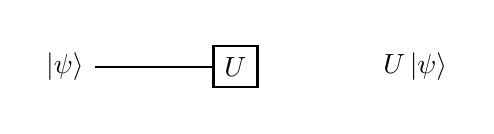
\begin{tikzpicture}
        \node[scale=1]{
        \begin{quantikz}
            \lstick{$\ket{\psi}$} &[1cm] \gate{U} &[1cm] \;U\ket{\psi}
        \end{quantikz}};
    \end{tikzpicture}
\end{figure}

以下に代表的な1量子ビットゲートを示す。計算基底によってユニタリ演算子を行列表示する。

% 1量子ビットに作用する $2\times2$ のユタニリ行列 $U$ は、$\mqty( \alpha & \beta \\ e^{i\varphi}\beta^* & -e^{i\varphi}\alpha^*),\, (|\alpha|^2 + |\beta|^2 =1)$ のように表される。\footnote{In general, $2\times2$ matrix can be given by $U = \smqty(a & b \\ c & d), \, a,b,c,d \in \bbC$. If the matrix is unitary, $UU\dg = \bbid \iff \abs{a}^2 + \abs{b}^2 = 1,\, \abs{c}^2 + \abs{d}^2 = 1,\, ac^* + bd^* = 0$. From the last condition, we see $ a:b = (-d^*):c^*$. Thus, $a = \alpha,\, b = \beta,\, c = e^{i\varphi}\beta^*,\, d = -e^{i\varphi}\alpha^*$ with $\abs{\alpha}^2 + \abs{\beta}^2 = 1$.}

\subsubsection{パウリゲート}
\begin{alignat}{3}
    \bbid &= \dyad{0} + \dyad{1}               &&= \paulii \\
    X &= \dyad{1}{0} + \dyad{0}{1}   &&= \paulix \\
    Y &= i\dyad{1}{0} - i\dyad{0}{1} &&= \pauliy \\
    Z &= \dyad{0} - \dyad{1}               &&= \pauliz
\end{alignat}

\subsubsection{Hadamard ゲート $H$、位相ゲート $S$、Tゲート $T$}
\begin{alignat}{5}
    H &= \dyad{+}{0} + \dyad{-}{1} &&= \frac{1}{\sqrt{2}}&&\mqty[1 & 1 \\ 1 & -1] \\
    S &= \dyad{0}{0} + i\dyad{1}{1} &&= &&\mqty[1 & 0 \\ 0 & i] \\
    T &= \dyad{0}{0} + e^{i\pi/4}\dyad{1}{1} &&= &&\mqty[1 & 0 \\ 0 & e^{i\pi/4}]
\end{alignat}
ただし、$\ket{\pm} := \frac{1}{\sqrt{2}}(\ket{0} \pm \ket{1})$ である。

\subsubsection{回転ゲート $R_x,\,R_y,\,R_z$}
$\bs{n}$ を3次元の単位ベクトル、$\bs{\sigma} = (X,Y,Z)$ をパウリ行列のベクトルとする。任意の正方行列 $A$ に対して、$\exp(iA\th) = \cos(\th)\bbid + i\,\sin(\th)A$ であることを用いると、$R_n := \exp(-i\th\,\bs{n\cdot\sigma}/2)$ を三角関数によって次のように表すことができる。
\begin{align}
    R_n := \exp(-i\th\,\bs{n\cdot\sigma}/2) = \cos(\frac{\th}{2})\bbid - i\,\sin(\frac{\th}{2})(\bs{n\cdot\sigma})
\end{align}

特に、$n = (1,0,0),\,(0,1,0),\,(0,0,1)$ のとき、$R_n$ は Bloch球面上で $x, y, z$ 軸周りの回転を表す。よって、これらの軸周りの回転を表すゲートを $R_x,\,R_y,\,R_z$ と定義する。
\begin{alignat}{3}
    R_x(\th) &:= e^{-i\th X/2} = \cos(\frac{\th}{2})\bbid -i\,\sin(\frac{\th}{2})X &&=  \rx{\th}\\
    R_y(\th) &:= e^{-i\th Y/2} = \cos(\frac{\th}{2})\bbid -i\,\sin(\frac{\th}{2})Y &&=  \ry{\th}\\
    R_z(\th) &:= e^{-i\th Z/2} = \cos(\frac{\th}{2})\bbid -i\,\sin(\frac{\th}{2})Z &&=  \rz{\th}
\end{alignat}

ブロッホ球面上の点は、直交する2つの軸周りの回転の合成で任意の点に移すことができる。よって、任意の1量子ビットゲートは、$R_x,\,R_y,\,R_z$ のいずれか2つの軸周りの回転の合成で表すことができる。

\subsection{制御ゲート}
制御ゲートとは、制御ビットが$\ket{1}$のときのみ、標的ビットにユニタリ演算子 $U$ を作用させるゲートである。制御ビットが$\ket{0}$のときは、標的ビットに何も作用させない。
この制御ゲートを用いることで、複数量子ビット間にエンタングルメント(\ref{sec:entanglement}~節)という量子力学的な相関を作り出すことができる。
一般に、第 $i$ 量子ビットを制御ビット、第 $j$ 量子ビットを標的ビットとする制御ゲートを $C_j^i[U]$ と表す。行列表示すると、
\begin{align}
    C_j^i[U] = \dyad{0}\ot \bbid + \dyad{1}\ot U
    = \mqty[
        1 & 0 & 0 & 0 \\
        0 & 1 & 0 & 0 \\
        0 & 0 & U_{11} & U_{12}\\
        0 & 0 & U_{21} & U_{22}
        ]
\end{align}

量子回路において、第 $i$ 量子ビットを制御ビット、第 $j$ 量子ビットを標的ビットとする制御ゲートを次のように表す。
\begin{figure}[H]
    \centering
    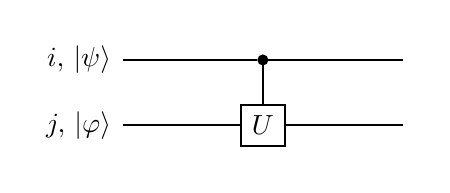
\begin{tikzpicture}
        \node[scale=1]{
        \begin{quantikz}
            \lstick{$i,\,\ket{\psi}$}    &[1cm] \ctrl{1} &[1cm] \qw \\
            \lstick{$j,\,\ket{\varphi}$} &[1cm] \gate{U} &[1cm] \qw
        \end{quantikz}};
    \end{tikzpicture}
\end{figure}

制御ビットと標的ビットは、複数の場合もある。例えば、$n$ 個の量子ビットのうち、$i_1,\,i_2,\,\cdots,\,i_k$ 番目の量子ビットを制御ビット、$j_1,\,j_2,\,\cdots,\,j_l$ 番目の量子ビットを標的ビットとする制御ゲートを $C_{j_1j_2\cdots j_l}^{i_1i_2\cdots i_k}[U]$ と表す。

\subsubsection{CNOT ゲート}
$U = X$ のときの制御ゲートを CNOT ゲートと呼ぶ。制御ビットが$\ket{1}$のときのみ、標的ビットにXゲートを作用させるゲートである。制御ビットと標的ビットを明示する場合は、$C_j^i[X]$ と表す。行列表示すると、
\begin{align}
    C_j^{i}[X] = \dyad{0}\ot \bbid + \dyad{1}\ot X
    = \mqty[
        1 & 0 & 0 & 0 \\
        0 & 1 & 0 & 0 \\
        0 & 0 & 0 & 1 \\
        0 & 0 & 1 & 0
        ]
\end{align}

量子回路において、第 $i$ 量子ビットを制御ビット、第 $j$ 量子ビットを標的ビットとする CNOT ゲートを次のように表す。
\begin{figure}[H]
    \centering
    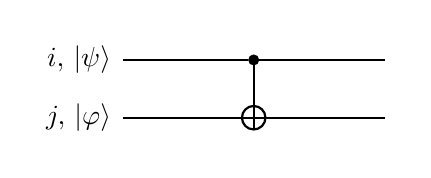
\begin{tikzpicture}
        \node[scale=1]{
        \begin{quantikz}
            \lstick{$i,\,\ket{\psi}$}    &[1cm] \ctrl{1} &[1cm] \qw \\
            \lstick{$j,\,\ket{\varphi}$} &[1cm] \targ{}  &[1cm] \qw
        \end{quantikz}};
    \end{tikzpicture}
\end{figure}



\subsubsection{SWAP ゲート}
2つの量子ビットの状態を入れ替えるゲートを SWAP ゲートと呼ぶ。つまり、$\SWAP \ket{\psi}\ot\ket{\varphi} = \ket{\varphi}\ot\ket{\psi}$ と作用する。
SWAP ゲートは、CNOT ゲートを3つ組み合わせて作ることができる。行列表示すると、
\begin{align}
    \SWAP = C_j^i[X]\,C_i^j[X]\,C_j^i[X]
    = \mqty[
        1 & 0 & 0 & 0 \\
        0 & 0 & 1 & 0 \\
        0 & 1 & 0 & 0 \\
        0 & 0 & 0 & 1
        ]
\end{align}

量子回路において、第 $i$ 量子ビットと第 $j$ 量子ビットの状態を入れ替える SWAP ゲートを次のように表す。
\begin{figure}[H]
    \centering
    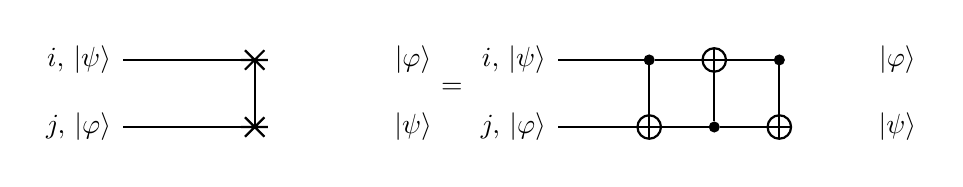
\begin{tikzpicture}
        \node[scale=1]{
        \begin{quantikz}
            \lstick{$i,\,\ket{\psi}$}    &[1cm] \swap{1} &[1cm] \;\ket{\varphi} \\
            \lstick{$j,\,\ket{\varphi}$} &[1cm] \targX{} &[1cm] \;\ket{\psi}
        \end{quantikz}
        =
        \begin{quantikz}
            \lstick{$i,\,\ket{\psi}$}    &[0.5cm] \ctrl{1} & \targ{}   & \ctrl{1} &[0.5cm] \;\ket{\varphi} \\
            \lstick{$j,\,\ket{\varphi}$} &[0.5cm] \targ{}  & \ctrl{-1} & \targ{}  &[0.5cm] \;\ket{\psi}
        \end{quantikz}
        % =
        % \begin{quantikz}
        %     \lstick{$i,\,\ket{\psi}$}    &[0.5cm] \targ{}   & \ctrl{1} & \targ{}   &[0.5cm] \qw \\
        %     \lstick{$j,\,\ket{\varphi}$} &[0.5cm] \ctrl{-1} & \targ{}  & \ctrl{-1} &[0.5cm] \qw
        % \end{quantikz}
        };
    \end{tikzpicture}
\end{figure}


\subsubsection{CZ ゲート}
$U = Z$ のときの制御ゲートを CZ ゲートと呼ぶ。制御ビットが $\ket{1}$ のときのみ、標的ビットにZゲートを作用させるゲートである。行列表示すると、
\begin{align}
    \CZ = \dyad{0}\ot \bbid + \dyad{1}\ot Z
    = \mqty[
        1 & 0 & 0 & 0 \\
        0 & 1 & 0 & 0 \\
        0 & 0 & 1 & 0 \\
        0 & 0 & 0 & -1
        ]
\end{align}

CZ ゲートは、計算基底 $\ket{11}$ のみに $-1$ をかけるゲートである。よって、制御ビットと標的ビットを入れ替えても CZ ゲートの作用は変わらないため、$C_j^i[Z] = C_i^j[Z]$ である。

量子回路において、第 $i$ 量子ビットを制御ビット、第 $j$ 量子ビットを標的ビットとする CZ ゲートを次のように表す。
\begin{figure}[H]
    \centering
    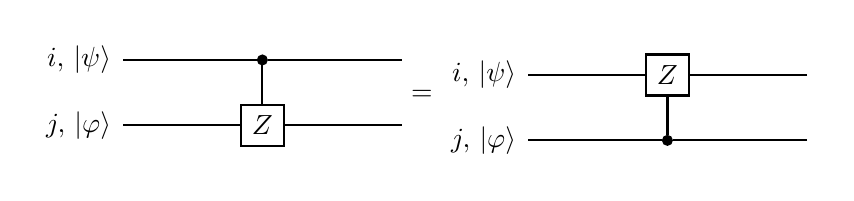
\begin{tikzpicture}
        \node[scale=1]{
        \begin{quantikz}
            \lstick{$i,\,\ket{\psi}$}    &[1cm] \ctrl{1} &[1cm] \qw \\
            \lstick{$j,\,\ket{\varphi}$} &[1cm] \gate{Z} &[1cm] \qw
        \end{quantikz}
        =
        \begin{quantikz}
            \lstick{$i,\,\ket{\psi}$}    &[1cm] \gate{Z}  &[1cm] \qw \\
            \lstick{$j,\,\ket{\varphi}$} &[1cm] \ctrl{-1} &[1cm] \qw
        \end{quantikz}
        };
    \end{tikzpicture}
\end{figure}


\subsubsection{Toffoli ゲート}
Toffoli ゲートは、2つの制御ビットと1つの標的ビットを持つ3量子ビットゲートである。2つの制御ビットがともに $\ket{1}$ のときのみ、標的ビットにXゲートを作用させるゲートである。CCX ゲートとも呼ばれる。制御ビットと標的ビットを明示する場合は、$C_k^{i,j}[X]$ と表す。行列表示すると、
\begin{align}
    C_k^{i,j}[X]
    &= \dyad{00}\ot \bbid + \dyad{01}\ot \bbid \nonumber\\
    &+ \dyad{10}\ot \bbid + \dyad{11}\ot X \nonumber\\
    &= \mqty[
        1 & 0 & 0 & 0 & 0 & 0 & 0 & 0 \\
        0 & 1 & 0 & 0 & 0 & 0 & 0 & 0 \\
        0 & 0 & 1 & 0 & 0 & 0 & 0 & 0 \\
        0 & 0 & 0 & 1 & 0 & 0 & 0 & 0 \\
        0 & 0 & 0 & 0 & 1 & 0 & 0 & 0 \\
        0 & 0 & 0 & 0 & 0 & 1 & 0 & 0 \\
        0 & 0 & 0 & 0 & 0 & 0 & 0 & 1 \\
        0 & 0 & 0 & 0 & 0 & 0 & 1 & 0
        ]
\end{align}

量子回路において、第 $i$ 量子ビットと第 $j$ 量子ビットを制御ビット、第 $k$ 量子ビットを標的ビットとする Toffoli ゲートを次のように表す。
\begin{figure}[H]
    \centering
    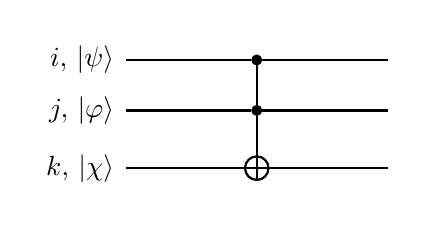
\begin{tikzpicture}
        \node[scale=1]{
        \begin{quantikz}
            \lstick{$i,\,\ket{\psi}$}    &[1cm] \ctrl{1} &[1cm] \qw \\
            \lstick{$j,\,\ket{\varphi}$} &[1cm] \ctrl{1} &[1cm] \qw \\
            \lstick{$k,\,\ket{\chi}$}    &[1cm] \targ{}  &[1cm] \qw
        \end{quantikz}};
    \end{tikzpicture}
\end{figure}



\section{測定}
量子コンピューターにおいて、測定は計算基底によって行われる。1量子ビットのある状態を測定して得られる結果は、計算基底のどちらかである。それぞれの計算基底が得られる確率は、その状態の計算基底の振幅の絶対値の2乗である。例えば、$\ket{\psi} = \alpha\ket{0} + \beta\ket{1}$ である状態を測定すると、0が出る確率は $|\alpha|^2$、1が出る確率は $|\beta|^2$ である。この確率分布を得るためには、多数回の測定を行う必要がある。
また、測定後の状態は、測定された計算基底に対応する状態となる。例えば、$\ket{\psi} = \alpha\ket{0} + \beta\ket{1}$ である状態を測定して0が出たとすると、測定後の状態は $\ket{0}$ になる。$n$ 量子ビットの場合も同様である。

量子回路において、第 $i$ 量子ビットを測定するときは、以下のように表す。
\begin{figure}[H]
    \centering
    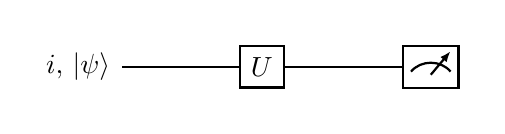
\begin{tikzpicture}
        \node[scale=1]{
        \begin{quantikz}
            \lstick{$i,\,\ket{\psi}$} &[1cm] \gate{U} &[1cm] \meter{}
        \end{quantikz}};
    \end{tikzpicture}
\end{figure}



\section{エンタングルメント}\label{sec:entanglement}
エンタングルメントとは、複数の量子ビットの状態が純粋状態であるにもかかわらず、それぞれの量子ビットの状態に分離して記述することができないような状態の性質である。例えば、次の2量子ビットの状態はエンタングルメントを持つ。
\begin{align}
    \ket{\psi_{\mathrm{ent}}} = \frac{1}{\sqrt{2}}(\kten{0}{0} + \kten{1}{1})
\end{align}
$\ket{\psi}$ は、$\kten{0}{0}$ と $\kten{1}{1}$ の重ね合わせであるが、それぞれの量子ビットの状態に分離した形、すなわち、$\ket{\phi} \otimes \ket{\varphi}$ の形で表すことができない。

量子計算は行列計算によって記述されるので、原理的には古典コンピューターでシミュレートすることができる。エンタングルメントのない分離可能な量子状態は、各量子ビットの状態を個別に記述できるので、古典コンピューターによる計算量は量子ビット数に関して線形に増える。
しかし、エンタングルメントを持つ量子状態の場合、各量子ビットの状態を個別に記述できないので、古典コンピューターによる計算量は量子ビット数に関して指数関数的に増える。
このように、エンタングルメントの存在が量子計算と古典計算の計算量の差を生み出す。



\section{量子状態の縮約}
量子状態の縮約とは、全体の系の量子状態からある部分系の量子状態を求める操作のことである。例えば、2量子ビットの状態 $\rho$ において第1量子ビットの状態 $\rho_1$ を求めるには、次のように $\rho$ の第2量子ビットの部分トレースを取ることで求めることができる。
\begin{align}
    \rho_1 = \Tr_2[\rho]
\end{align}

例として、2量子ビットの系を考える。全体の系の状態 $\rho$ が各量子ビットの状態のテンソル積で表される、つまり、$\rho = (\ket{\psi_1}\otimes\ket{\psi_2})(\bra{\psi_1}\otimes\bra{\psi_2}) = \dyad{\psi_1} \otimes \dyad{\psi_2}$ とする。このとき、第1量子ビットの状態は、
\begin{align*}
    \rho_1 = \Tr_2[\dyad{\psi_1} \otimes \dyad{\psi_2}] = \dyad{\psi_1} \Tr[\dyad{\psi_2}] = \dyad{\psi_1}
\end{align*}
である。これは純粋状態である。

一方、全体の系の状態 $\rho$ がエンタングルメントを持ち、次の状態で表されるとする。
\begin{align*}
    \rho &= \dyad{\psi_{\mathrm{ent}}}\\
    &= \frac{1}{2}\qty(\kten{0}{0} + \kten{1}{1})(\bten{0}{0} + \bten{1}{1})\\
    &= \frac12(\dyad0\ot\dyad0 + \dyad{0}{1}\ot\dyad{0}{1} + \dyad{1}{0}\ot\dyad{1}{0} + \dyad1\ot\dyad1) 
\end{align*}
このとき、第1量子ビットの状態は、
\begin{align*}
    \rho_1 &= \Tr_2[\dyad{\psi_{\mathrm{ent}}}]\\
    &= \frac12(\dyad0\Tr[\dyad0] + \dyad{0}{1}\Tr[\dyad{0}{1}] + \dyad{1}{0}\Tr[\dyad{1}{0}] + \dyad1\Tr[\dyad1])\\
    &= \frac12(\dyad0 + \dyad1)\\
    &= \frac{\bbid}{2}
\end{align*}
である。これは最大混合状態である。このように、エンタングルメントを持つ量子状態の部分系の状態は、混合状態になることがある。



\begin{comment}
\section{フィデリティー}
フィデリティーとは、2つの量子状態がどれだけ近いかを表す尺度である。密度演算子 $\rho$ と $\sigma$ のフィデリティーは次のように定義される。
\begin{align}
    F(\rho, \sigma) := \Tr\sqrt{\sqrt{\sigma}\rho\sqrt{\sigma}} \in [0,\,1]
\end{align}

例えば、$\rho = \sigma$ のとき、$F(\rho, \sigma) = 1$ である。一方、$\rho = \dyad{0}$, $\sigma = \dyad{1}$ のとき、$F(\rho, \sigma) = 0$ である。

% \begin{align}
%     F(\rho, \sigma) := \Tr|\sqrt{\rho}\sqrt{\sigma}| = \Tr\sqrt{(\sqrt{\rho}\sqrt{\sigma})\dg\sqrt{\rho}\sqrt{\sigma}}= \Tr\sqrt{\sqrt{\sigma}\rho\sqrt{\sigma}}
% \end{align}
% $\rho,\,\sigma$ は半正定値行列であるから、$\sqrt{\rho},\,\sqrt{\sigma}$ も半正定値行列である。よって、
% $$
%     \sqrt{\rho}\dg = \sqrt{\rho}, \sqrt{\sigma}\dg = \sqrt{\sigma} \rightarrow (\sqrt{\rho}\sqrt{\sigma})\dg = \sqrt{\sigma}\sqrt{\rho}.
% $$

% フィデリティーは、$F(\rho, \sigma) := (\Tr\sqrt{\sqrt{\rho}\sigma\sqrt{\rho}})^2$ と定義されることもある。

% 任意のユニタリ演算子 $U$ と任意の密度演算子 $A$ に対して、$\sqrt{UAU\dg} = U\sqrt{A}U\dg$ \footnote{任意のユニタリ演算子 $U$ と任意の演算子 $B$ に対して、$(UBU\dg)^2 = UB^2U\dg$ が成り立つ。よって、$B = \sqrt{A}$ とおくと、$U\sqrt{A}U\dg = \sqrt{UAU\dg}$ である。} が成り立つことから、
% $$
%     F(U\rho U\dg, U\sigma U\dg) = \Tr\sqrt{\sqrt{U\sigma U\dg}U\rho U\dg\sqrt{U\sigma U\dg}} = \Tr\qty[U\sqrt{\sqrt{\sigma}\rho\sqrt{\sigma }}U\dg] = F(\rho, \sigma).
% $$
% すなわち、ユニタリ変換に対してフィデリティーは不変である。
% フィデリティーが1に近いほど、2つの状態は絶対位相を除いて近いことを表す。

% $\sigma$ が純粋状態のとき、$\sigma = \dyad{\varphi} \rightarrow \sqrt{\sigma} = \dyad{\varphi}$ であるから、
% \begin{align*}
%     F(\rho, \sigma) &:= \Tr|\sqrt{\rho}\sqrt{\sigma}|\\
%     &= \Tr\sqrt{\sqrt{\sigma}\rho\sqrt{\sigma}}\\
%     &= \Tr[(\bra{\varphi}\rho\ket{\varphi}\dyad{\varphi})^{1/2}]\\
%     &= \sqrt{\bra{\varphi}\rho\ket{\varphi}}\Tr(\dyad{\varphi})\\
%     &= \sqrt{\bra{\varphi}\rho\ket{\varphi}}.
% \end{align*}

% 特に、$\rho,\,\sigma$ がともに純粋状態であり、$\sigma = \dyad{\varphi}$, $\rho = \dyad{\psi}$ とすると、忠実度は次のようになる。
% $$
%     F(\rho, \sigma) = \abs{\bra{\psi}\ket{\varphi}}.
% $$


% Properties of fidelity
% \begin{enumerate}
%     \item $ 0 \leq F(\rho, \sigma) \leq 1 \,\, (F(\rho, \sigma)=1 \Leftrightarrow \rho = \sigma)$
%     \item $F(\rho, \sigma) = F(\sigma, \rho)$
%     \item $\sigma$ が純粋状態 $\dyad{\varphi}$ である時、$F(\rho, \sigma) = \sqrt{\bra{\varphi}\rho\ket{\varphi}}$
%     \item for any CPTP map $\Lambda$, $F(\rho, \sigma) \leq F(\Lambda(\rho), \Lambda(\sigma))$
%     \item  when $\rho$ and $\sigma$ commyte, and $ \rho=\sum_i p_i\dyad{i},\, \sigma=\sum_i q_i\dyad{i}$, $$F(\rho, \sigma) = \sum_i \sqrt{p_i q_i}$$ (fidelity for classical probability distribution)
% \end{enumerate}
\end{comment}


\section{Schatten $p$--ノルム}\label{sec:schatten-norm}
\begin{screen}
    \begin{definition}
        $A \in \calL(\calH)$ のSchatten $p$--ノルムは次のように定義される。
        \begin{equation}
            \norm{A}_p = 
            \begin{cases}
                \qty(\Tr[\abs{A}^p])^{\frac1p} & (1 \leq p < \infty) \\
                \lambda_{\max}(\abs{A}) & (p = \infty)
            \end{cases}
        \end{equation}
        ここで $\abs{A} = \sqrt{A\dg A}$ であり、$\lambda_{\max}(\abs{A})$ は $\abs{A}$ の最大固有値である。
    \end{definition}
\end{screen}


$A, B \in \calL(\calH)$ とする。Schatten $p$--ノルムは以下の性質を持つ。
\begin{enumerate}
    \item $1 \leq \fa p \leq \fa q \leq \infty$ に対して $\norm{A}_q \leq \norm{A}_p$
    \item $\fa p \in [1, \infty],\,\,\fa U,V\in\calU(d)$ に対して $\norm{UAV\dg}_p = \norm{A}_p$
    \item $\norm{A}_p = \norm{A\T}_p = \norm{A^*}_p = \norm{A\dg}_p$
    \item $1\leq \fa p, q, r$ and $1/p + 1/q \leq 1/r$ に対して $\norm{AB}_r \leq \norm{A}_p \norm{B}_q$ (H\"olderの不等式)
    \begin{itemize}
        \item 例1 $\norm{AB}_1 \leq \norm{A}_1 \norm{B}_\infty$.
        \item 例2 $\norm{AB}_1 \leq \norm{A}_2 \norm{B}_2$.
    \end{itemize}
\end{enumerate}

% \section{トレース距離}
% まず、行列 $A$ のトレースノルムを次のように定義する。
% \begin{align}
%     \norm{A}_1 = \Tr|A| = \Tr\sqrt{A\dg A} = \sum_{i=1}^n |\lambda_i|
% \end{align}

% トレース距離は次のように定義される。
% \begin{align}
%     D_{\Tr}(A,B) = \norm{A-B}_1 := \Tr\sqrt{(A-B)\dg(A-B)}
% \end{align}


\section{Hilbert--Schmidt 距離}
$A, B \in \calL(\calH)$ の Hilbert--Schmidt 距離を次のように定義する。
\begin{align}
    D_{\HS}(A, B) := \norm{A - B}_{\HS}^2 = \Tr [(A - B)\dg(A - B)]
\end{align}

$X$ がエルミート演算子のとき、$ X\dg = X $ であるから、密度演算子 $\rho,\,\sigma$ の Hilbert--Schmidt 距離は
\begin{align}
    D_{\HS}(\rho, \sigma) = \norm{\rho - \sigma}_{\HS}^2 = \Tr [(\rho - \sigma )^2] \,\in [0,\,2]
\end{align}
となる。
例えば、$\rho = \sigma$ のとき $D_{\HS}(\rho, \sigma) = 0$ であり、$\rho = \dyad{0}\otn{n},\, \sigma = \dyad{1}\otn{n} $ のとき $D_{\HS}(\rho, \sigma) = 2$ である。
また、$\rho$ と最大混合状態 $\bbid/d$ ($d = 2^n$) の Hilbert--Schmidt 距離は、
\begin{align}
    D_{\HS}(\rho,\, \bbid/d) &= \Tr\qty[(\rho - \bbid/d)^2]\nonumber\\
    &= \Tr\qty[ \rho^2 - 2\rho\cdot \bbid/d + \bbid/d^2 ]\nonumber\\
    &= \Tr[\rho^2] - \frac{1}{d} \,\in [0,\, 1 - 1/d]
\end{align}
となる。特に、$\rho = \dyad{\psi}$ のとき $D_{\HS}(\dyad{\psi},\, \bbid/d) = 1 - 1/d$ である。

% 上記の距離を用いて、純粋状態からの距離を次のように定義する~\cite{sharma2021geometric}。
% \begin{align}
%     U_{\HS}(\rho) &= D_{\HS}(V\dyad{\psi}V\dg,\, \bbid/d) - D_{\HS}(\rho,\, \bbid/d)\\
%     &= 1 - \Tr[\rho^2]
% \end{align}
% この量は、線形エントロピーとも呼ばれ、量子状態の純粋性を表す量として用いられる。



\section{量子ノイズ}
量子ノイズには、コヒーレントなノイズとデコヒーレントなノイズの2種類がある。コヒーレントなノイズは、量子状態の純粋度を変化させないが、位相を変化させるノイズである。デコヒーレントなノイズは、量子状態の純粋度を変化させるノイズである。ここでは、後者の例を紹介する。

\subsection*{ビット反転チャネル}
ビット反転チャネルとは、確率 $p$ で量子ビットに $X$ ゲートを作用させるチャネルであり、1量子ビットに対して次のように定義される。
\begin{align}
    \calN_p(\rho) := (1 - p)\rho + pX{\rho}X
\end{align}
式\eqref{eq:density-operator-1qubit}にて確認したように、$\rho = \frac12(\bbid + r_x X + r_y Y + r_z Z)$ と表せることから、
$X{\rho}X = \frac12(\bbid + r_x X - r_y Y - r_z Z)$ となる。これは、ブロッホ球上の点 $(r_x,\,r_y,\,r_z)$ を $x$ 軸まわりに $\pi$ 回転させることに相当する。
これと同様に、$y$ 軸まわりに $\pi$ 回転させるチャネルと $z$ 軸まわりに $\pi$ 回転させるチャネルを定義することができ、それぞれ、ビット位相反転チャネル、位相反転チャネルと呼ばれる。

\subsection*{Depolarizing チャネル}\label{sec:depolarizing-channel}
Depolarizing チャネルは、ビット反転チャネル、位相反転チャネル、ビット位相反転チャネルを含むチャネルであり、1量子ビットに対して次のように定義される。
\begin{align}
    \calN_p(\rho) := \qty(1 - \frac34p)\rho + \frac{p}{4}(X{\rho}X + Y{\rho}Y + Z{\rho}Z)
\end{align}

ここで、次の等式が成り立つ。
\begin{align}
    X{\rho}X &= \frac12(\bbid + r_x X - r_y Y - r_z Z)\nonumber\\
    Y{\rho}Y &= \frac12(\bbid - r_x X + r_y Y - r_z Z)\\
    Z{\rho}Z &= \frac12(\bbid - r_x X - r_y Y + r_z Z)\nonumber
\end{align}
これより、
\begin{align}
    \frac{\bbid}{2} = \frac{\rho + X\rho X + Y\rho Y + Z\rho Z}{4}
\end{align}
であるから、Depolarizing チャネルは次のように書き換えることができる。
\begin{align}
    \calN_p(\rho)
    &= (1 - p)\rho + p\,\frac{\bbid}{2}
\end{align}

例えば、$p  = \frac12$ のとき、Depolarizing チャネルは図~\ref{fig:depolarizing-channel}ように、ブロッホ球面上の点 $(r_x,\,r_y,\,r_z)$ を収縮するように変化させるチャネルである。
\begin{figure}[H]
    \centering
    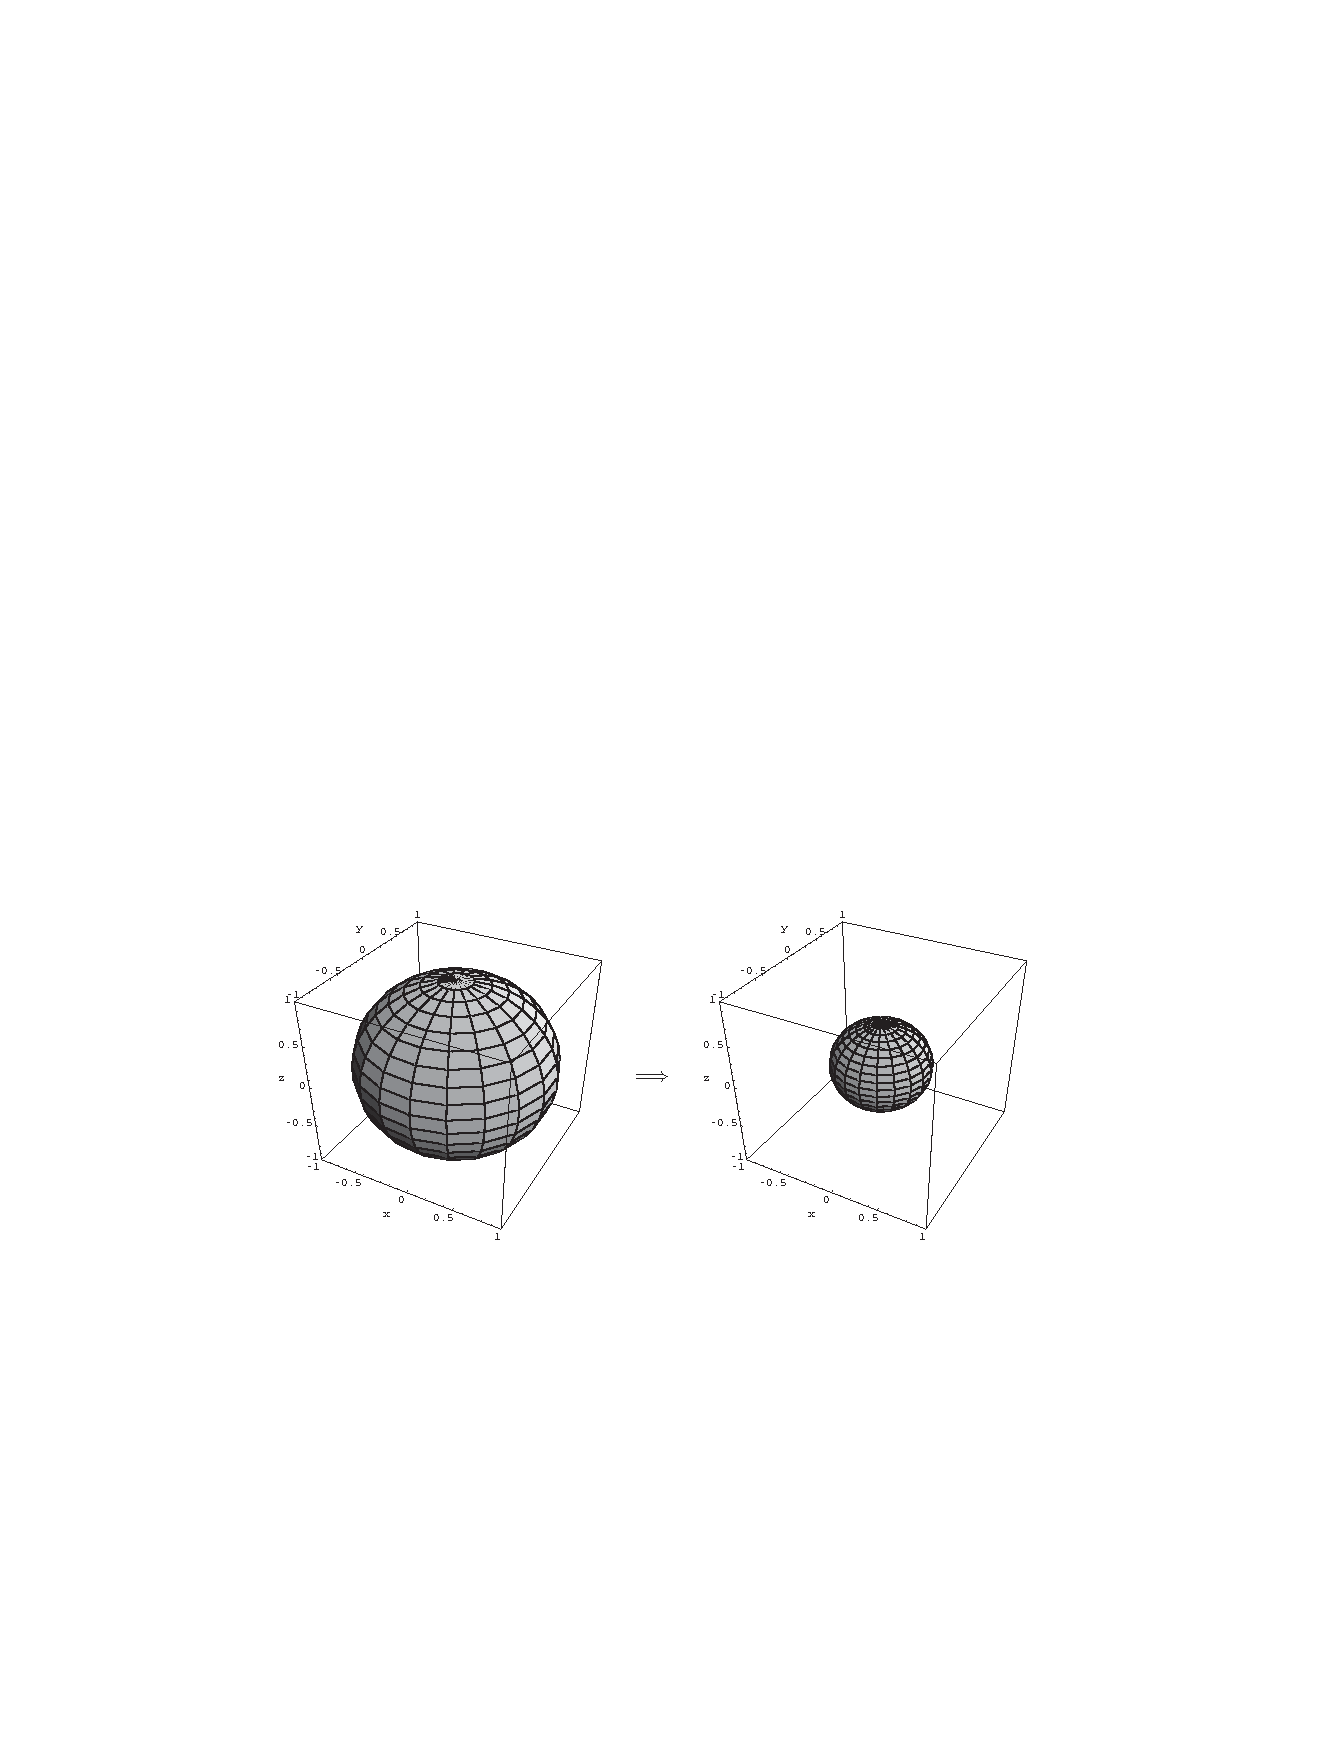
\includegraphics[width=15cm]{depolarizing-channel.pdf}
    \caption{Depolarizing channel~\cite{nielsen2010quantum}}
    \label{fig:depolarizing-channel}
\end{figure}

$n$ 量子ビットに対する Depolarizing チャネルは、次のように定義される。
\begin{align}
    \calN_p(\rho) = (1 - p)\rho + p\,\frac{\bbid}{2^n}
\end{align}
% これは、各量子ビットに対して Depolarizing チャネルを作用させることとは異なる。

\subsection*{Depolarizing チャネルによる量子ノイズモデル}
量子コンピューター上で、$n$ 量子ビットの初期状態 $\rho$ に対して、$L$ 個のユニタリ演算子を作用させることを考える。このとき、各ユニタリ演算子に付随して、Depolarizing チャネル $\calN_{p_i}$ が作用すると仮定する。作用させるユニタリチャネルを $\calE_i(\rho) = U_i\rho U_i\dg,\, i = 1,\,2,\,\cdots,\,L$ とすると、全体のチャネル $\calN$ は次のように表される。
\begin{align}
    \calN(\rho) = \qty(\bigcirc_{i=1}^L \calN_{p_i} \circ \calE_i)(\rho)
\end{align}
ここで、次のように $\calN_{p_i} \circ \calE_i = \calE_i \circ \calN_{p_i}$ が成り立つ。
\begin{align}
    \calN_{p_i} \circ \calE(\rho)
    = (1-p_i)(U\rho U\dg) + p_i\,\frac{\bbid}{2^n}
    = U\qty((1-p_i)\rho + p_i\,\frac{\bbid}{2^n})U\dg
    = \calE \circ \calN_{p_i}(\rho)
\end{align}

よって、$\calE := \bigcirc_{i=1}^L \calE_i$,  $\calN_{\bs{p}}^L := \bigcirc_{i=1}^L \calN_{p_i},\; \bs{p} = (p_1,\,p_2,\,\cdots,\,p_L)$ とすると、
\begin{align}
    \calN
    = \bigcirc_{i=1}^L \calN_{p_i} \circ \calE_i
    = \qty(\bigcirc_{i=1}^L \calN_{p_i}) \circ \qty(\bigcirc_{i=1}^L \calE_i)
    = \calN_{\bs{p}}^L \circ \calE
\end{align}
となる。つまり、$\calN$ は、$\calE$ の後に $\calN_{\bs{p}}^L$ が作用することと同じである。
簡単のため、$p_i = p$ とすると、$\calN_p^L(\rho)$ は次のように計算される。
\begin{align}
    \calN_{\bs{p}}^L(\rho) = (1 - p)^L\rho + \{1 - (1 - p)^L\}\,\frac{\bbid}{2^n}
\end{align}

このとき、次の $\calN$ を得る。
\begin{align}
    \calN(\rho)
    = \calN_{\bs{p}}^L \circ \calE(\rho)
    = (1 - p)^L\calE(\rho) + \{1 - (1 - p)^L\}\,\frac{\bbid}{2^n}
\end{align}



\newpage
\chapter{変分量子アルゴリズム}\label{chap:vqa}
この章では、NISQ 上でも実行可能なアルゴリズムとして現在盛んに研究されいてる変分量子アルゴリズムについて説明する。\ref{sec:vqc}~節では、変分量子アルゴリズムをコスト関数・変分量子回路・最適化の3つ部分に分けて説明する。\ref{sec:qml}~節では、量子機械学習について説明する。\ref{sec:bp}~節では、バレンプラトーについて説明する。

\section{概要}\label{sec:vqc}
現在実現されている量子コンピューターは、中規模(数百量子ビット)であり、ノイズが大きいため、Noisy Intermediate Scale Quantum computers (\ruby{NISQ}{ニスク})と呼ばれている\cite{preskill2018quantum}。このため、使用できる量子ビットと量子ゲートの数に制約がある。そのような制約のもと、古典計算よりも効率的に計算を行うことを期待されているのが、変分量子アルゴリズムである。
変分量子アルゴリズムは、古典コンピューターと組み合わせて最適化問題を解くアルゴリズムである。最適化問題とは、ある関数の値を最小化するようなパラメーターの値を求める問題である。
変分量子アルゴリズムでは、パラメーターに依存した量子状態によってオブザーバブルの期待値を計算し、それを用いて定義されたコスト関数 $C(\bs{\th})$ を最適化することによって問題を解く。
パラメーターの更新を古典コンピューターに任せることで、量子回路を浅く保つことができる。図\ref{fig:vqa-flow}のように、量子状態の生成からパラメーターの更新までのサイクルを繰り返すことで、最終的に最適なパラメーター$\bs{\th}_* = \argmin_{\bs{\th}} C(\bs{\th})$ を得る。試行関数を生成するパラメーター付き量子回路のことを、変分量子回路、アンザッツ(Ansatz)、あるいは、量子ニューラルネットワーク(Quanum Neural Network, QNN)と呼ぶ。
\begin{figure}[H]
    \centering
    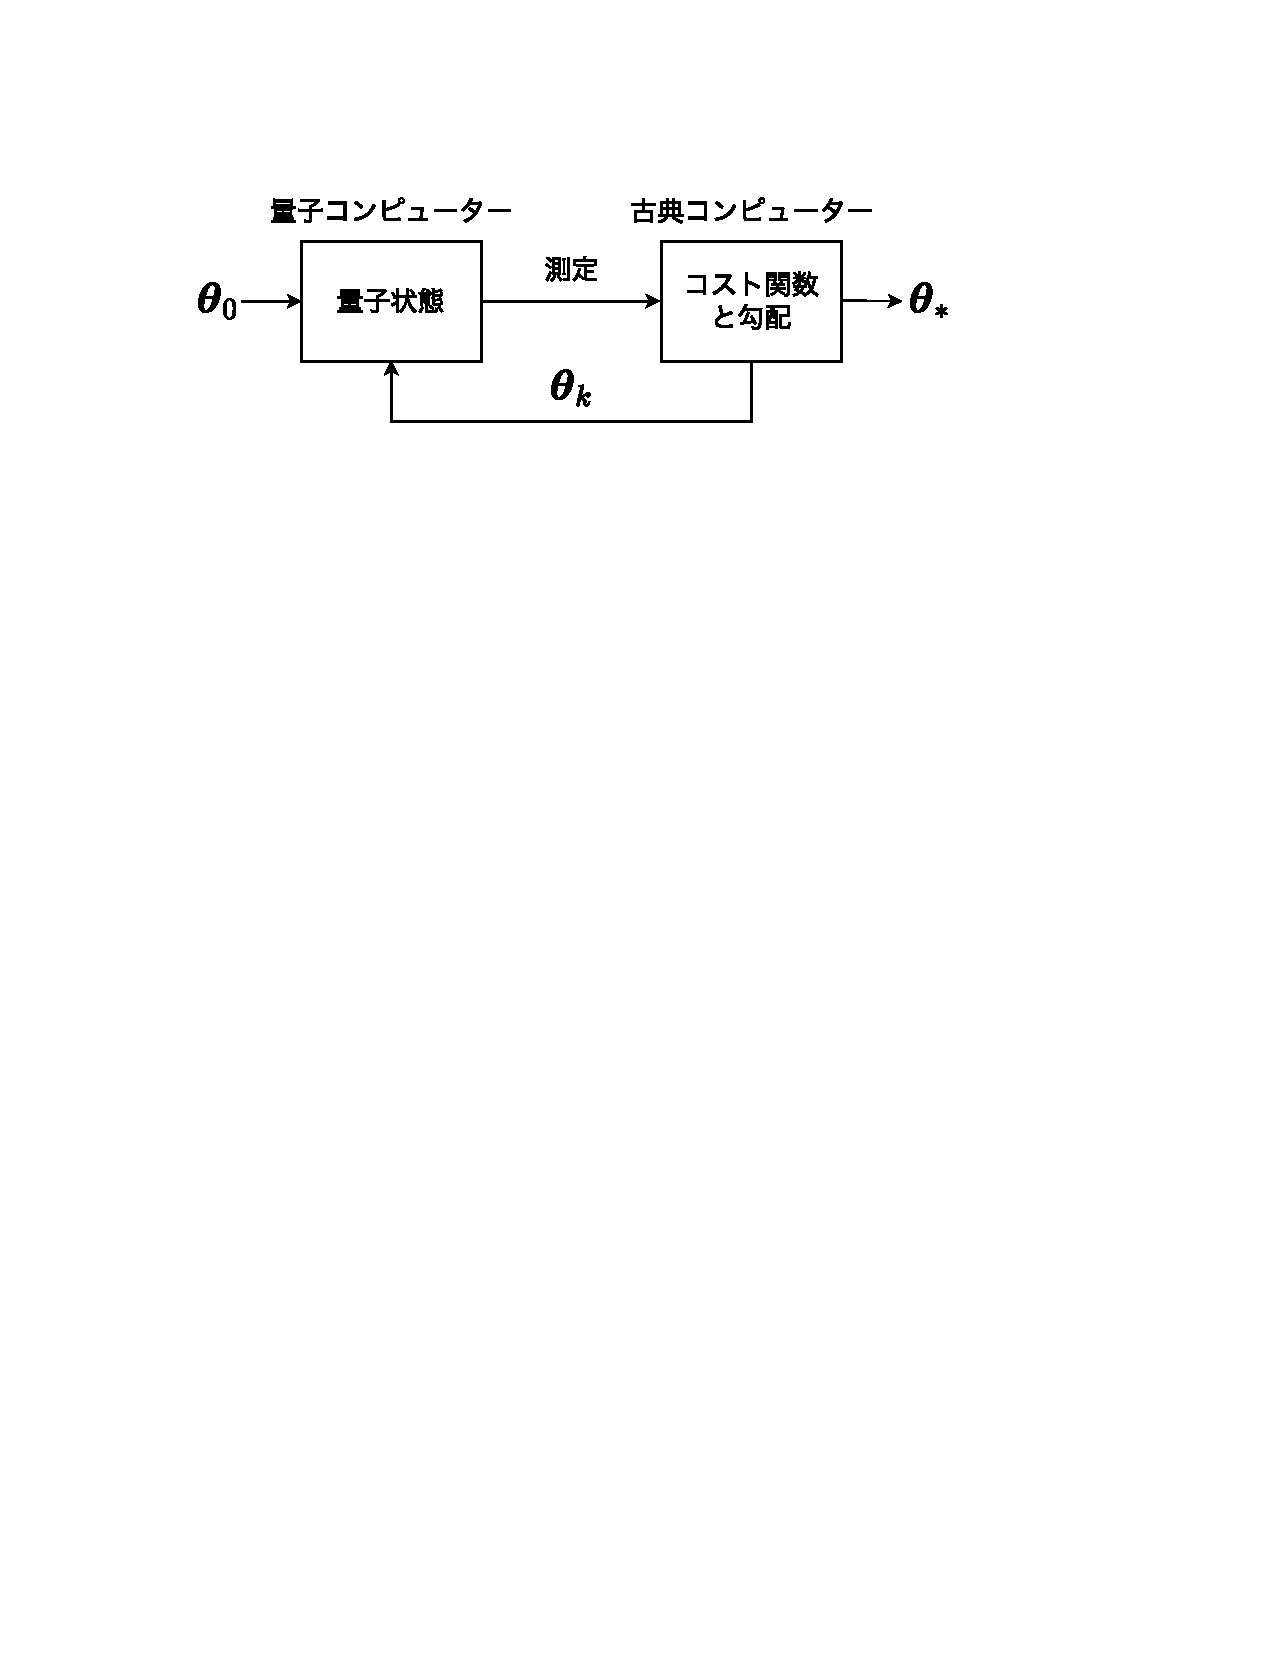
\includegraphics[width=12cm]{vqa-flow.pdf}
    \caption{変分量子アルゴリズムの概要}
    \label{fig:vqa-flow}
\end{figure}

ある問題を解くための変分量子アルゴリズムを構成するには、以下の3つの要素が必要である。
\begin{enumerate}
    \item 解きたい問題をコスト関数の最適化問題として定式化すること
    \item コスト関数を最適化するための変分量子回路を構成すること
    \item パラメーターを最適化するための最適化手法を選択すること
\end{enumerate}
これらについて、順に説明する。

\subsection{コスト関数}\label{sec:cost}
変分量子アルゴリズムにおけるコスト関数は、初期状態の集合 $\{\rho_i\}$、変分量子回路 $V(\bs{\th})$、オブザーバブルの集合 $\{O_k\}$ を用いて定義される。変分量子回路を作用させた状態 $V(\bs{\th}) \rho_i V\dg(\bs{\th})$ によるオブザーバブル $O_k$ の期待値は、
\begin{align}
    \Tr[V(\bs{\th}) \rho_i V\dg(\bs{\th}) O_k]
\end{align}
である。
コスト関数は、この期待値を用いて定義される。
ほとんどのコスト関数は、$f$ を任意の関数として次のような形で与えられる。
\begin{align}\label{eq:cost-general}
    C(\bs{\th}) = f\qty(\qty{\Tr[V(\bs{\th}) \rho_i V\dg(\bs{\th}) O_k]}_{i,k})
\end{align}

コスト関数は、その最小点が求める解に対応するように設計する。
例えば、変分量子固有値ソルバー (Variational Quantum Eigensolover, VQE) では、ハミルトニアンが $H$ で与えられる系の最小エネルギーを求めるために、$\rho_i = \dyad{\psi_0}$, $O_k = H$ とする。このとき、コスト関数は以下のように定義される。
\begin{align}\label{eq:cost-vqe}
    C(\bs{\th}) = \bra{\psi_0}V\dg(\bs{\th}) H V(\bs{\th})\ket{\psi_0}
\end{align}

また、変分量子回路を用いた機械学習(量子機械学習)では、データセット $\{(\bs{x}_i, y_i)\}_{i=1}^N$ が与えられたとき、入力状態を $\rho_i = U({\bs{x}_i})\dyad{0}U\dg({\bs{x}_i})$, オブザーバブルを $O_k = O$ として、各データに依存するオブザーバブルの期待値 $\Tr[V(\bs{\th}) \rho_i V\dg(\bs{\th}) O]$ が対応するラベル $y_i$ になるように、以下のようなコスト関数を定義することができる。
\begin{align}\label{eq:cost-qml}
    C(\bs{\th}) = \frac1N\sum_{i=1}^N \qty(\Tr[V(\bs{\th}) \rho_i V\dg(\bs{\th}) O] - y_i)^2
\end{align}


\subsection{変分量子回路}
一般に、変分量子回路 $V(\bs{\th})$ は、回転ゲートなどのパラメーター付き量子ゲートと CNOT ゲートなどのパラメーターなし量子ゲートの積で表すことができる。$U_j(\bs{\th}_j)$ を任意の数のパラメーター付き量子ゲートからなるユニタリ、$W_j$ を任意の数のパラメーターなし量子ゲートからなるユニタリであるとすると、$V(\bs{\th})$ は次のように表わすことができる。
\begin{align}
    V(\bs{\th})
    = \prod_{j=1}^{L} U_j(\bs{\th}_j) W_j
    = U_L(\bs{\th}_L)W_L\cdots U_1(\bs{\th}_1)W_1
\end{align}
変分量子回路においては、類似した構造を複数回繰り返すことがあり、その構造単位の繰り返しの数を層数と呼び、この数が多いほど深い回路であるという。図~\ref{fig:vqc}は $L$ 層の変分量子回路を表している。

\newcommand{\wj}[1]{\gate[wires=3]{{\LARGE W_{#1}}}}
\newcommand{\uj}[1]{\gate[wires=3]{{\LARGE U_{#1}(\th_{#1})}}}
\begin{figure}[H]
    \centering
    \begin{quantikz}
        \lstick{$\ket{0}$}    & \wj{1}& \uj{1} & \wj{2}& \uj{2}& \ \cdots\ & \wj{L}& \uj{L}& \meter{}\\
        \lstick{$\vdots\;\;$} & \wn   & \wn    & \wn   & \wn   & \wn\cdots & \wn   & \wn   & \wn\rstick{$\vdots$}\\
        \lstick{$\ket{0}$}    &       &        &       &       & \ \cdots\ &       &       & \meter{}
    \end{quantikz}
    \caption{$L$ 層の変分量子回路}
    \label{fig:vqc}
\end{figure}

アンザッツの構造は、問題の性質に応じて様々なものが考えられる。問題の対称性や制約を構造に取り入れたアンザッツを Problem-inspired アンザッツと呼ぶ。例えば、Quantum Alternating Operator Ansatz (QAOA) は組合せ最適化問題に対して提案された Problem-inspired アンザッツである。
一方、問題の性質に依存しないアンザッツを Problem-agnostic アンザッツと呼ぶ。

Hardware Efficient Ansatz は量子コンピューターの実機の構造を考慮し、実装が効率的にできるよう設計された Problem-agnostic アンザッツである。例えば、量子ビット $q_1,\,q_2,\,q_3,\,q_4$ が隣り合うインデックスのみ実機上でつながっているときに、図~\ref{fig:hea}のような回路の構造を持つアンザッツである。
これにより、実機上で隣り合わない量子ビットを結ぶための量子ゲートを実装する必要がなくなり、使用するSWAPゲートの数が減る。SWAP ゲートは CNOT ゲート3つから成るが、CNOT ゲートは量子ゲートの中でも特にノイズが多い。そのため、SWAP ゲートを減らすことはノイズの対策として有用である。

\begin{figure}[H]
    \centering
    \begin{quantikz}
        \lstick{$q_1$} & \gate{U(\th_1)} & \ctrl{1}&  \qw    & \qw     & \gate{U(\th_5)} & \ctrl{1}&  \qw    & \qw     & \gate{U(\th_9)}    & \ctrl{1} &  \qw    & \qw     & \meter{} \\
        \lstick{$q_2$} & \gate{U(\th_2)} & \targ{} & \ctrl{1}& \qw     & \gate{U(\th_6)} & \targ{} & \ctrl{1}& \qw     & \gate{U(\th_{10})} & \targ{} & \ctrl{1}& \qw     & \meter{} \\
        \lstick{$q_3$} & \gate{U(\th_3)} & \qw     & \targ{} & \ctrl{1}& \gate{U(\th_7)} & \qw     & \targ{} & \ctrl{1}& \gate{U(\th_{11})} & \qw     & \targ{} & \ctrl{1}& \meter{} \\
        \lstick{$q_4$} & \gate{U(\th_4)} & \qw     &   \qw   & \targ{} & \gate{U(\th_8)} & \qw     &   \qw   & \targ{} & \gate{U(\th_{12})} & \qw     &   \qw   & \targ{} & \meter{}
    \end{quantikz}
    \caption{Hardware Efficient Ansatz}
    \label{fig:hea}
\end{figure}


\subsection{最適化}\label{sec:optimization}
最適化とは、コスト関数を最小化するパラメーターを求めることであり、変分量子アルゴリズムでは古典コンピューターによって行われる。
最適化のアルゴリズムのことを、オプティマイザーと呼ぶ。
変分量子アルゴリズムにおいては、従来の古典計算で用いられるオプティマイザーをそのまま用いることができるが、量子計算に合わせて改良されたオプティマイザーも提案されている。オプティマイザーには、ノイズや測定誤差に強いものを選択する必要がある。

オプティマイザーには、コスト関数の勾配を用いるものと、用いないものに大別される。
勾配を用いるオプティマイザーには、勾配降下法、ニュートン法、量子自然勾配法\cite{stokes2020quantum}、確率的勾配降下法\cite{sweke2020stochastic}、Adam\cite{kingma2017adam}、などの方法がある。
勾配自体は、有限差分法やパラメーターシフトルール\cite{mitarai2018quantum,schuld2019evaluating}によって求めることができる。
例えば、勾配降下法では、パラメーター $\th_j$ を以下のように更新する。
\begin{align}
    \th_j \leftarrow \th_j - \alpha \pdv{C(\bs{\th})}{\th_j}
\end{align}
ここで、$\alpha$ は1回の更新でのパラメーターの変化量を決める、学習率と呼ばれるハイパーパラメーターである。通常、学習率は小さい正の値に設定されるが、適切な値は扱う問題によって異なる。

勾配を用いない方法では、コスト関数の値のみを用いてパラメーターを更新する。例えば、Nelder-Mead\cite{nelder1965simplex}、Powell\cite{powell1964efficient}、COBYLA (Constrained Optimization By Linear Approximation optimizer)\cite{powell1994direct}、SPSA (Simultaneous Perturbation Stochastic Approximation)\cite{spall1992multivariate}、逐次最小化問題最適化法\cite{platt1998sequential,nakanishi2020sequential,parrish2019jacobi,ostaszewski2021structure}などが挙げられる。

\subsubsection*{パラメーターシフトルール}\label{sec:parameter-shift-rule}
変分量子アルゴリズムにおいては、すべてのパラメーターが独立であれば、パラメーターシフトルールと呼ばれる手法によって、厳密に勾配を求めることができる\cite{mitarai2018quantum,schuld2019evaluating}(測定誤差は除く)。パラメーターシフトルールは、パラメーター付き量子ゲート $V(\bs{\th})$ によるオブザーバブルの期待値のパラメーター $\th_j$ に関する勾配を、パラメーター $\th_j$ を一定値ずらして得た期待値の差として求める方法である。

\begin{screen}
    \begin{theorem}
        (パラメーターシフトルール~\cite{mitarai2018quantum,schuld2019evaluating})
        % $U(\bs{\th}) := \prod_{i=1}^L U_i(\th_i)W_i = U_L(\th_L)W_L\cdots U_1(\th_1)W_1$
        量子回路 $V(\bs{\th})$ はパラメーター付き量子ゲート $U_j(\th_j) := \exp(-i\th_j P_j/2)$ とパラメーターなし量子ゲート $W_j$ によって $V(\bs{\th}) := U_L(\th_L)W_L\cdots U_1(\th_1)W_1$ と定義される。ここでは、すべてのパラメーターは独立であるとする。このとき、あるオブザーバブル $O$ の期待値 $\expval{O(\bs{\th})} = \Tr[V(\bs{\th})\dyad{0}\otn{n}V\dg(\bs{\th}) O]$ の $\th_j$ に関する勾配は
        \begin{align}
            \pdv{\expval{O(\bs{\th})}}{\th_j}
            = \frac{1}{2}\qty[\expval{O\qty({\bs{\th}}+\frac{\pi}{2}\bs{e}_j)}
            - \expval{O\qty({\bs{\th}}-\frac{\pi}{2}\bs{e}_j)}]
        \end{align}
        で与えられる。ここで $\bs{e}_j$ は $j$ 番目の方向の単位ベクトルである。
    \end{theorem}
\end{screen}

\begin{comment}
\begin{proof}
    パラメーター付き量子ゲートに対して、$U_{k:i} := U_k(\th_k)W_k \cdots U_i(\th_i)W_i$ という記法を用いる。
    $\pd_{\th_j}U_j(\th_j) = -\frac{i}{2}P_jU_j(\th_j)$ であることから、$B(\bs{\th})$ の $\th_j$ に関する勾配は、
    \begin{align}
        \pdv{\expval{B(\bs{\th})}}{\th_j}
        &= \pdv{\th_j} \Tr[BU_{L:1}\rho_{in} U_{L:1}\dg]\\
        &= \Tr[B \pdv{U_{L:1}}{\th_j} \rho_{in} U_{L:1}\dg] + \Tr[B U_{L:1} \rho_{in} \pdv{U_{L:1}\dg}{\th_j}]\\
        &= \Tr[B \qty(-\frac{i}{2}U_{L:j-1}P_jU_{j:1}) \rho_{in} U_{L:1}\dg] + \Tr[B U_{L:1} \rho_{in} \qty(\frac{i}{2}U_{j:1}\dg P_jU_{L:j-1}\dg)]\\
        &= -\frac{i}{2}\Tr[BU_{L:j-1}[P_j,U_{j:1}\rho_{in} U_{j:1}\dg]U_{L:j-1}\dg]
    \end{align}
    ここで、$U_j(\pm\pi/2) = (1/\sqrt{2})(\bbid\mp iP_j)$ であることから、
    \begin{align}
        [P_j,\rho^\prime] = i\qty[U_j\qty(\frac{\pi}{2})\rho^\prime\, U_j\qty(\frac{\pi}{2}) - U_j\qty(-\frac{\pi}{2})\rho^\prime\, U_j\qty(-\frac{\pi}{2})]
    \end{align}
    が成り立つ。
    よって、
    \begin{align}
    & U_{L:j-1}[P_j,U_{j:1}\rho_{in} U_{j:1}\dg]U_{L:j-1}\dg\\
    &= iU_{L:j-1}\qty[U_j\qty(\frac{\pi}{2})U_{j:1}\rho_{in} U_{j:1}\dg U_j\qty(\frac{\pi}{2}) - U_j\qty(-\frac{\pi}{2})U_{j:1}\rho_{in} U_{j:1}\dg U_j\qty(-\frac{\pi}{2})]U_{L:j-1}\dg\\
    &= i\Big[U_{L:j}U_j\qty(\th_j + \frac{\pi}{2})U_{j-1:1}\rho_{in} U_{j-1:1}\dg U_j\qty(\th_j + \frac{\pi}{2})U_{L:j}\dg\\
    &\quad - U_{L:j}U_j\qty(\th_j - \frac{\pi}{2})U_{j-1:1}\rho_{in} U_{j-1:1}\dg U_j\qty(\th_j - \frac{\pi}{2})U_{L:j}\dg\Big]
    \end{align}
    以上より、
    \begin{align}
        \pdv{\expval{B(\bs{\th})}}{\th_j}
        &= \frac{1}{2}\qty[ BU\qty(\bs{\th} + \frac{\pi}{2}\bs{e}_j)\rho U\dg\qty(\bs{\th} + \frac{\pi}{2}\bs{e}_j)
        - BU\qty(\bs{\th} - \frac{\pi}{2}\bs{e}_j)\rho U\dg\qty(\bs{\th} - \frac{\pi}{2}\bs{e}_j)]\\
        &= \frac{1}{2}\qty[\expval{B\qty(\bs{\th} + \frac{\pi}{2}\bs{e}_j)}
        - \expval{B\qty(\bs{\th} - \frac{\pi}{2}\bs{e}_j)}]
    \end{align}
\end{proof}
\end{comment}

より高次の勾配も同様に計算することができる。例えば、$V(\bs{\th})$ の $\th_j$ と $\th_k$ に関する勾配は、
\begin{align}
    \pdv{\expval{O(\bs{\th})}}{\th_j}{\th_k}
    = \frac12\qty[\eval{\pdv{\expval{O(\bs{\th})}}{\th_j}}_{\th_k = \th_k + \frac{\pi}{2}}
    - \eval{\pdv{\expval{O(\bs{\th})}}{\th_j}}_{\th_k = \th_k - \frac{\pi}{2}}]
\end{align}
で与えられる。

一般的なコスト関数 \eqref{eq:cost-general} の勾配については、連鎖律を用いると、
\begin{align}
    \pdv{C(\bs{\th})}{\th_j}
    = \pdv{\th_j}f\qty(\qty{\Tr[V(\bs{\th}) \rho_i V\dg(\bs{\th}) O_k]}_{i,k})
    = \sum_{i,k}\pdv{f}{\ell_{i,\bs{\th},k}}\pdv{\ell_{i,\bs{\th},k}}{\th_j}
\end{align}
となるので、$\ell_{i,\bs{\th},k}$ にパラメーターシフトルールを用いて勾配を計算することができる。
ここで、$\ell_{i,\bs{\th},k} := \Tr[V(\bs{\th}) \rho_i V\dg(\bs{\th}) O_k]$ とした。



\section{量子機械学習}\label{sec:qml}
近年、機械学習\footnote{機械学習の概要については付録の\ref{sec:machine-learning}~節に置いた。}はさまざまな分野で著しい成果を上げているが、その一方で、高い計算コストが問題となっている。そこで、機械学習の計算を量子コンピューター上で行い、計算を効率化できないか研究されている。そのような研究分野を量子機械学習(Quantum Machine Learning, QML)と呼ぶ。
量子機械学習におけるアルゴリズムの研究アプローチは次の3つがあげられる\cite{guan2021quantum}。
\begin{enumerate}
    \item 古典的な学習方法から量子的なものへの再構築
    \item 古典的な学習方法に勝る新たな量子機械学習の方法の探索
    \item 近い将来に向けた、NISQに特化した学習方法の探索
\end{enumerate}

2009年、Harrow, Hassidim, Lloyd は線形方程式を解く量子アルゴリズム(HHLアルゴリズム)を提案した~\cite{harrow2009quantum}。このアルゴリズムは、古典的なアルゴリズムよりも効率的に線形方程式を解くことが期待される量子アルゴリズムである。量子機械学習の初期の研究は、機械学習における線形代数の問題を HHL アルゴリズムによって量子コンピューター上で解くことに焦点を当てていた(1のアプローチ)。しかし、HHLアルゴリズムは量子位相推定を用いており、量子ビットと量子ゲートが数多く必要であるため、NISQ で実現できるアルゴリズムではなかった。
変分量子アルゴリズムが登場したことにより、その文脈で量子機械学習の研究が盛んになった(3のアプローチ)。
この節では、変分量子アルゴリズムとして研究されている3つの教師あり量子機械学習モデルについて説明する。量子回路学習(Quantum Circuit Learning)\cite{mitarai2018quantum,farhi2018classification}、Data reuploading\cite{perez-salinas2020data,lloyd2020quantum,schuld2021effect}、量子カーネル法(Quantum Kernel Methods)\cite{havlicek2019supervised,schuld2019quantum,schuld2021supervised}である。いずれのモデルも、図\ref{fig:vqa-flow}にある流れに従って学習を行うが、量子回路で行う計算が異なる。

\subsection{量子回路学習}\label{sec:quantum-circuit-learning}
\begin{figure}[H]
    \centering
    \begin{quantikz}
        \lstick{$\ket{0}$}     & \gate[wires=3][3cm]{{\LARGE U(\bs{x}_i)}} & \gate[wires=3][3cm]{{\LARGE V(\bs{\th})}} & \meter{}\\
        \lstick{$\vdots\;\;$}  & \wn &\wn & \wn\rstick{$\vdots$}\\
        \lstick{$\ket{0}$}     &     & \qw & \meter{}
    \end{quantikz}
    \caption{量子回路学習における量子回路の構造}
    \label{fig:qcl-circuit}
\end{figure}
% \begin{figure}[H]
%     \centering
%     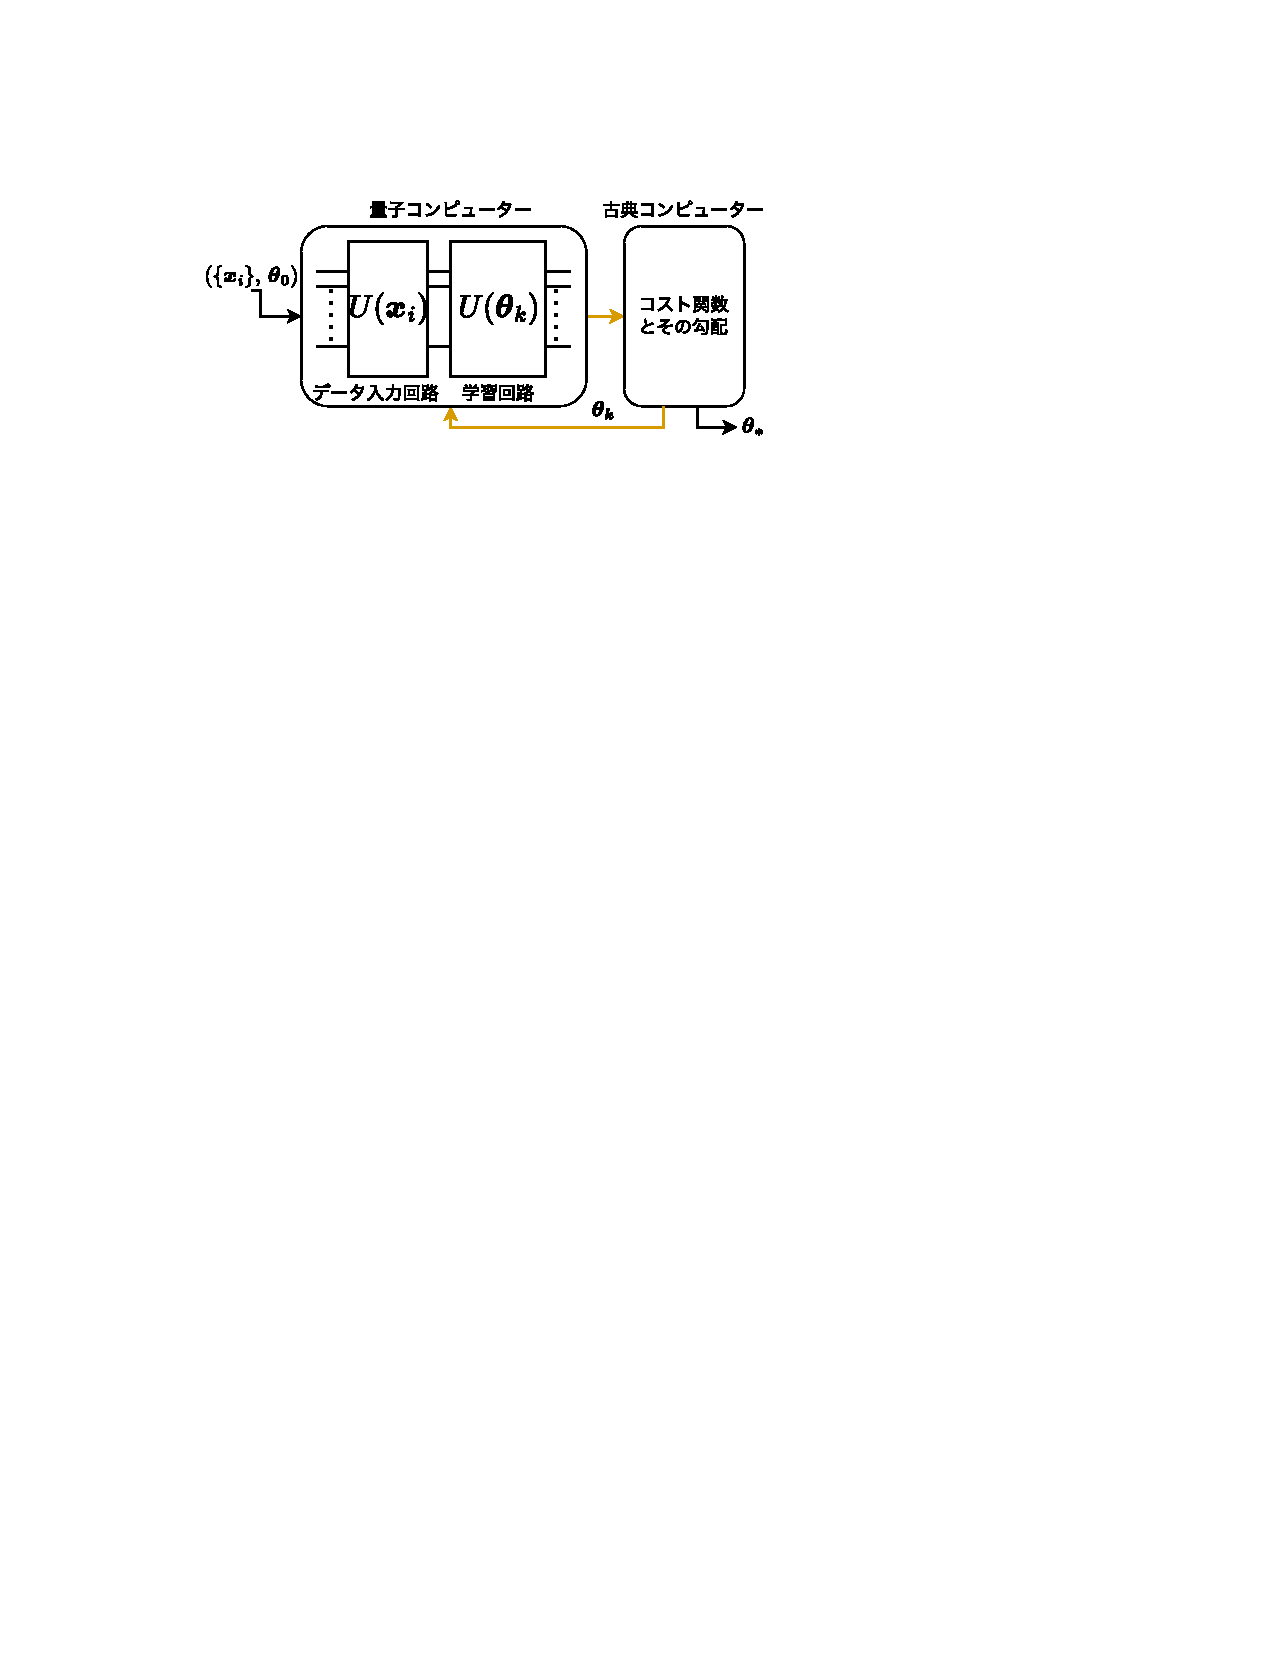
\includegraphics[width=12cm]{qml-alg.png}
%     \caption{量子回路学習の概要}
%     \label{fig:qml-alg}
% \end{figure}

図\ref{fig:qcl-circuit}は量子回路学習における量子回路の構造を表している。まず、初期状態 $\ket{0}\otn{n}$ にデータを入力するためのユニタリ $U(\bs{x}_i)$ を作用させ、続いて、学習パラメーターを入力するためのユニタリ $V(\bs{\th})$ を作用させる。前者を入力回路、後者を学習回路と呼ぶことにする。これにより、状態 $V(\bs{\th})U(\bs{x}_i)\ket{0}\otn{n}$ が生成される。
そして、この状態によって測定したオブザーバブルの期待値 $\{\Tr[V(\bs{\th})U(\bs{x}_i)\dyad{0}\otn{n}U\dg(\bs{x}_i)V\dg(\bs{\th}) O_k]\}_k$ を用いて、\ref{eq:cost-qml}のようなコスト関数が定義される。
古典コンピューター上では、コスト関数とその勾配を計算し、学習パラメーターを更新する。
このプロセスを繰り返すことで、最適なパラメーター $\bs{\th}_\ast$ を得る。
後の第\ref{chap:upper-bound},\ref{chap:lower-bound}章において扱う量子機械学習のモデルも、この量子回路学習に基づいて解析を行う。



\subsection{Data reuploading}\label{sec:data-reuploading}
\newcommand{\Ux}[1]{\gate[wires=3][1cm]{{\Large U_{#1}(\bs{x}_i,\bs{\th}_{#1})}}}
\begin{figure}[H]
    \centering
    \begin{quantikz}
        \lstick{$\ket{0}$}    &\Ux{1}&\Ux{2}&\ \ldots\    &\Ux{L}& \meter{}\\
        \lstick{$\vdots\;\;$} &\wn   &\wn   &\wn\ \ldots\ &\wn   & \wn\rstick{$\vdots$}\\
        \lstick{$\ket{0}$}    &\qw   &\qw   &\ \ldots\    &\qw   & \meter{}
    \end{quantikz}
    \caption{Data reuploading における量子回路の構造}
    \label{fig:data-reuploading}
\end{figure}

量子回路学習とは異なり、いくつかの研究においては、データの入力と学習パラメーターの入力を交互に繰り返す量子回路\cite{schuld2021effect,lloyd2020quantum}や、一つのゲートにデータと学習パラメーターの線形和を入力する量子回路\cite{perez-salinas2020data}が用いられている。このような量子回路の構造は、Data reuploading と呼ばれている(図~\ref{fig:data-reuploading})。コスト関数の定式化は、量子回路学習と同様である。




\subsection{量子カーネル法}\label{sec:quantum-kernel}
\begin{figure}[H]
    \centering
    \begin{quantikz}
        \lstick{$\ket{0}$} & \gate[wires=3][3cm]{{\LARGE U(\bs{x}_i)}} & \gate[wires=3][3cm]{{\LARGE U\dg(\bs{x}_j)}} & \meter{}\\
        \lstick{$\vdots\;\;$}  & \wn & \wn & \wn\rstick{$\vdots$}\\
        \lstick{$\ket{0}$} & & \qw & \meter{}
    \end{quantikz}
    \caption{量子カーネル法における量子回路の構造}
    \label{fig:quantum-kernel}
\end{figure}

カーネル法は、入力データを高次元の特徴空間に写像し、その空間での内積を用いることで非線形な分類や回帰を行う機械学習である。カーネル法のコスト関数は凸であり、局所的な解に陥ることがないので、量子回路学習と Data reuploading による機械学習よりも、学習が安定すると期待されている\cite{schuld2021supervised}。
量子カーネル法では、カーネルの計算のみを量子コンピューター上で行う\cite{havlicek2019supervised,schuld2019quantum}。
例えば、データ $\bs{x}_i,\bs{x}_j$ に依存する量子状態
\begin{align*}
    \rho(\bs{x}_i) := U(\bs{x}_i)\dyad{0}\otn{n}U\dg(\bs{x}_i),\\
    \rho(\bs{x}_j) := U(\bs{x}_j)\dyad{0}\otn{n}U\dg(\bs{x}_j)
\end{align*}
を用いて定義される量子カーネル(Fidelity Quantum Kernel)$\kappa_{FQ}(x_i,x_j) := \Tr[\rho(x_i)\rho(x_j)]$ を計算するための量子回路は図\ref{fig:quantum-kernel}で与えられる。
初期状態 $\ket{0}\otn{n}$ に対してユニタリ $U(\bs{x}_i), U\dg(\bs{x}_j)$ を順に作用させて、状態 $U\dg(\bs{x}_j)U(\bs{x}_i)\ket{0}\otn{n}$ を作り、$\dyad{0}\otn{n}$ によって測定を行う。これによって得られる期待値は、確かに $\Tr[\rho(\bs{x}_i)\rho(\bs{x}_j)]$ に等しい。
\begin{align}
    \Tr[U\dg(\bs{x}_j)U(\bs{x}_i)\dyad{0}\otn{n}(U\dg(\bs{x}_j)U(\bs{x}_i))\dg\dyad{0}\otn{n}]
    = \Tr[\rho(\bs{x}_i)\rho(\bs{x}_j)]
\end{align}

しかしながら、量子カーネル $\kappa_{FQ}(\bs{x_i},\bs{x_j})$ は、訓練可能性\footnote{訓練可能性(Trainability)とは、最適化ができるかどうかということである。量子カーネル $\kappa_{FQ}(\bs{x_i},\bs{x_j})$ は定義からグローバルオブザーバブル $\dyad{0}\otn{n}$ を用いるため、勾配消失(バレンプラトー)が生じ、最適化が困難になる。詳しくは次の節を参照。}、
汎化性能が悪いことが知られている\cite{thanasilp2022exponential,huang2021power,kubler2021inductive}。
そのため、Bandwidth $\lambda$ を導入した量子カーネル $\kappa_{FQ}^\lambda(\bs{x_i},\bs{x_j}) := \kappa_{FQ}(\lambda \bs{x_i},\lambda \bs{x_j})$ を用いること\cite{shaydulin2022importance,canatar2023bandwidth}や、
次式で定義されるカーネル(Projected Quantum Kernel)$\kappa_{PQ}(\bs{x_i},\bs{x_j})$ が用いることが提案されている\cite{huang2021power}。
\begin{align}
    \kappa_{PQ}(\bs{x_i},\bs{x_j}) := \exp(- \gamma\sum_{i=1}^{n}\norm{\rho^{(k)}(\bs{x_i}) - \rho^{(k)}(\bs{x_j})}_2^2)
\end{align}
ただし、$\rho^{(k)}(\bs{x_i})$ は、$k$ 番目の量子ビットにおける縮約密度演算子である。


\section{バレンプラトー}\label{sec:bp}
\subsection{概要}
変分量子アルゴリズムにおいては、いくつかの原因によってバレンプラトーと呼ばれるコスト関数の勾配消失(平坦化)が起こりうる\cite{mcclean2018barren}。バレンプラトーに陥ると、量子回路のパラメーターの更新に量子ビット数に関して指数関数的な計算量が必要となるため、古典計算以上の効率化は不可能である。この節では、バレンプラトーの定義、原因、提案されている回避方法について述べる。
まず初めに、バレンプラトーの定義を与える。
% \begin{screen}
    % \begin{definition}
    %     $\rho(\bs{\th})$ をパラメーター $\bs{\th}$ に依存する密度行列、$O$ を任意のオブザーバブルとし、コスト関数は $C(\bs{\th}) = \Tr[\rho(\bs{\th}) O]$ と表されるとする。\\
    %     確率論的なバレンプラトーとは、コスト関数 $C(\bs{\th})$ が以下の性質を持つことを指す。
    %     \begin{align}
    %         \Pr\qty[\abs{\pdv{C(\bs{\th})}{\th_\nu}} \geq \fa\delta > 0] \leq \frac{\epsilon}{\delta^2}
    %     \end{align}
    %     決定論的なバレンプラトーとは、コスト関数 $C(\bs{\th})$ が以下の性質を持つことを指す。
    %     \begin{align}
    %         \abs{\pdv{C(\bs{\th})}{\th_\nu}} \leq \epsilon
    %     \end{align}
    %     ただし、量子ビット数を $n$ として $\epsilon \in \order{1/b^n}, \,\, 1 < \ex b$ である。
    % \end{definition}
% \end{screen}
% 確率論的なバレンプラトーの定義は、次のように言い換えることができる。

\begin{screen}
    \begin{definition}\label{def:bp}
        バレンプラトーとは、コスト関数 $C(\bs{\th})$ のあるパラメーター $\th_\nu$ に関する勾配が次の性質を持つことである\cite{mcclean2018barren}。
        \begin{align}
            \E_{V(\bs{\th})}\qty[\pdv{C(\bs{\th})}{\th_\nu}] = 0\,, \quad \Var_{V(\bs{\th})}\qty[\pdv{C(\bs{\th})}{\th_\nu}] \in \order{2^{-\alpha n}}\,, \quad 0 < \ex \alpha
        \end{align}
    \end{definition}
\end{screen}

このように、バレンプラトーとは、コスト関数の勾配の平均が0になり、勾配の分散が量子ビット数に関して指数関数的に小さくなる現象を指す。
$X$ を確率変数とすると、$\fa\delta > 0$ に対して次のチェビシェフの不等式が成り立つ。
\begin{align}
    \Pr[\,|X - \E[X]| \geq \delta] \leq \frac{\Var[X]}{\delta^2}
\end{align}

コスト関数の勾配を確率変数とみなすと、チェビシェフの不等式より、
\begin{align}
    \Pr\qty[\abs{\pdv{C(\bs{\th})}{\th_\nu}} \geq \delta]
    \leq \frac{1}{\delta^2}\Var_{V(\bs{\th})}\qty[\pdv{C(\bs{\th})}{\th_\nu}] \in \order{2^{-\alpha n}}
\end{align}
となる。
よって、量子ビット数を増やすにつれて、勾配が0から離れる確率が指数関数的に小さくなることがわかる。
変分量子アルゴリズムにおいて、パラメーターの初期値として適当なものがわからない場合、しばしば初期値はランダムに選ばれる。バレンプラトーが起きる場合、ほとんどの初期値は勾配が $0$ の平坦な領域にあるため、最適化は難しい。

これを視覚的に示したものが図~\ref{fig:bp-cost-1}である。バレンプラトーが起きるとき、あるパラメーターに関するコスト関数の断面は、量子ビット数が多いほど平坦な領域(勾配がほぼ0)が増え、狭い谷(narrow gorge)を持つ\cite{arrasmith2022equivalence}。

\begin{figure}[H]
    \centering
    \begin{tikzpicture}[scale=1.5]
        \def\a{1}
        \def\b{0.8}
        \def\c{0.1}
        \def\d{2.2}
        \draw [->] (0,2.7) -- (9,2.7) node [right]{{\Large $n$}};
        \draw [domain=0:4,smooth] plot (\x,{-2*\b^2/(\b^2 + (\x-2)^2) + \d});
        \draw [domain=5:9,smooth] plot (\x,{-2*\c^2/(\c^2 + (\x-7)^2) + \d});
        % \draw [->,thick] (0,2.7) -- (9.5,2.7) node [right]{n};
        \draw [->] (0,0) -- (4,0) node [right]{{\Large $\th_k$}};
        \draw [->] (5,0) -- (9,0) node [right]{{\Large $\th_k$}};
    \end{tikzpicture}
    \caption{Noise-free バレンプラトーにおけるコスト関数の断面の変化のイメージ}
    \label{fig:bp-cost-1}
\end{figure}

定義\ref{def:bp}によるバレンプラトーのことを Noise-free バレンプラトー、あるいは確率論的なバレンプラトーと呼ぶ。一方で、論文\cite{mcclean2018barren}の後に示されたような、ノイズが原因のバレンプラトーのことを Noise-induced バレンプラトー、あるいは決定論的なバレンプラトーと呼ぶ。この場合、コスト関数の勾配の大きさが、層数 $L$ に関して指数関数的に小さくなる\cite{wang2021noiseinduced}。特に、$L \in \order{n}$ のとき、次のようになる。
\begin{align}
    \abs{\pdv{C(\bs{\th})}{\th_\nu}} \in \order{2^{-\alpha n}}\,, \quad 0 < \ex \alpha
\end{align}
これを視覚的に示したものが図~\ref{fig:bp-cost-2}である。コスト関数全体が収縮しているため、さらに最適化が難しくなる。

\begin{figure}[H]
    \centering
    \begin{tikzpicture}[scale=1.5]
        \def\a{1}
        \def\b{0.8}
        \def\c{0.2}
        \def\d{2.2}
        \draw [->] (0,2.7) -- (9,2.7) node [right]{{\Large $L$}};
        \draw [domain=0:4,smooth] plot (\x,{-2*\b^2/(\b^2 + (\x-2)^2) + \d});
        \draw [domain=5:9,smooth] plot (\x,{\c*(-2*\b^2/(\b^2 + (\x-7)^2)) + \d-1});
        % \draw [domain=5:9,smooth] plot (\x,{-2*\c^2/(\c^2 + (\x-7)^2) + \d});
        % \draw [->,thick] (0,2.7) -- (9.5,2.7) node [right]{n};
        \draw [->] (0,0) -- (4,0) node [right]{{\Large $\th_k$}};
        \draw [->] (5,0) -- (9,0) node [right]{{\Large $\th_k$}};
    \end{tikzpicture}
    \caption{Noise-induced バレンプラトーにおけるコスト関数の断面の変化のイメージ}
    \label{fig:bp-cost-2}
\end{figure}


そもそも、コスト関数やその勾配は測定によってのみ得られるため、測定誤差が必ず存在する。
もし、その測定誤差によってコスト関数の勾配の推定値と実際の勾配の正負が逆になると、最適化が進まない。
測定回数が $N_{\text{shot}}$ の場合、測定誤差は $\order{1/\sqrt{N_{\text{shot}}}}$ である。バレンプラトーが起きる場合、コスト関数の勾配の分散は指数関数的に小さくなるため、その値の正負を判別するには、測定誤差も指数関数的に小さくする必要がある。これは、測定回数を指数関数的に増やす必要があることを意味する。

変分量子アルゴリズムの目的は、コスト関数を最小化するパラメーターを、量子ビット数の高々多項式の計算量で求めることである。バレンプラトーが起きる場合、コスト関数の最小点を量子ビット数の多項式の計算量で求めることはできない。
高次の勾配に関しても、同様の現象が見られることが示されている~\cite{cerezo2021higher}。また、勾配を用いないオプティマイザーを用いる場合でも、必要な測定回数は量子ビット数に関して指数関数的に増えることが知られている~\cite{arrasmith2021effect}。これを表しているのが、図~\ref{fig:bp-var}である。したがって、オプティマイザーを変えることでバレンプラトーを回避することはできない。
\begin{figure}[H]
    \centering
    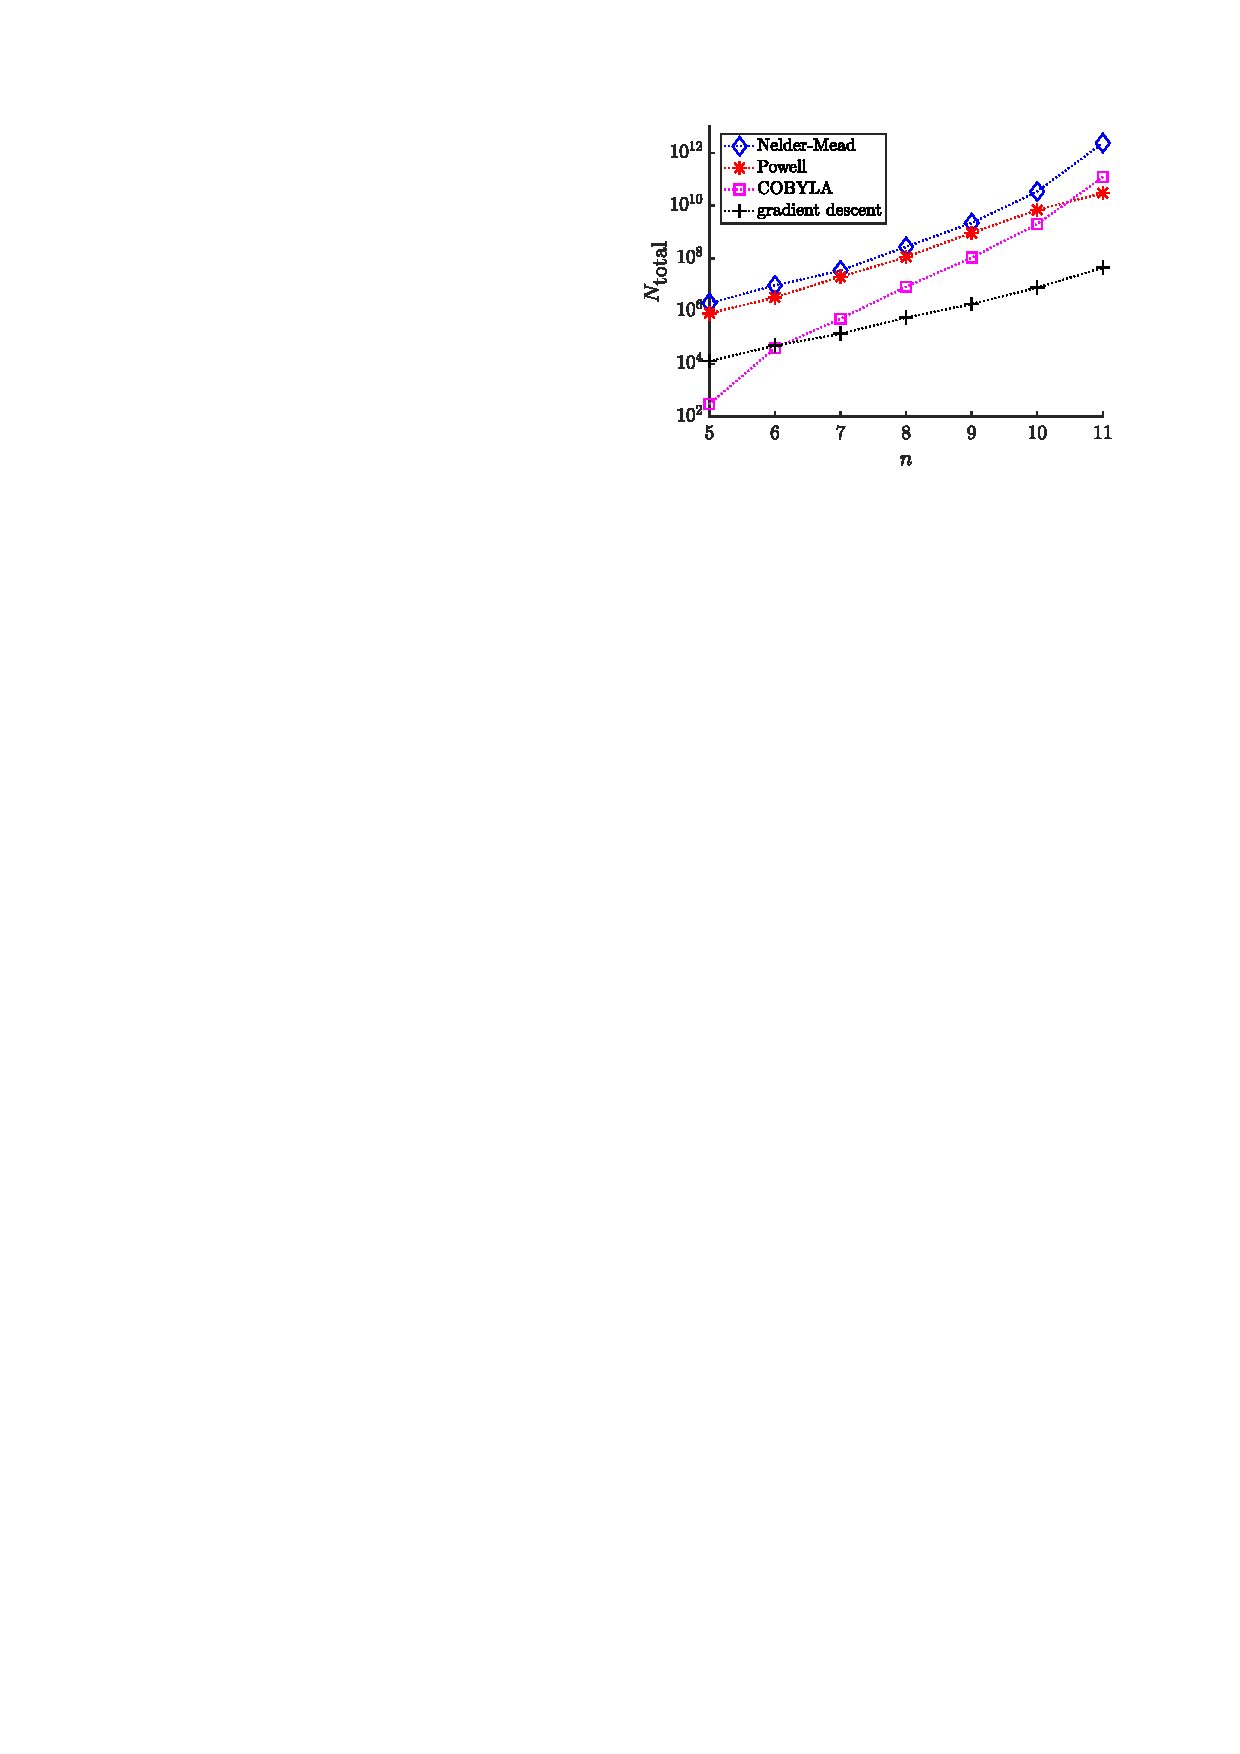
\includegraphics[width=12cm]{bp-nshots.pdf}
    \caption{バレンプラトーにおいて必要なオブザーバブルの測定回数 $N_{\text{total}}$の量子ビット数 $n$ に対する変化~\cite{arrasmith2021effect}。Nelder-Mead・Powell・COBYLA は勾配を用いないオプティマイザーである。}
    \label{fig:bp-var}
\end{figure}


% 実際にバレンプラトーが起きているときに必要な測定回数の変化を、図~\ref{fig:bp-var}に示す。
% \begin{figure}[H]
%     \label{fig:bp-var}
%     \centering
%     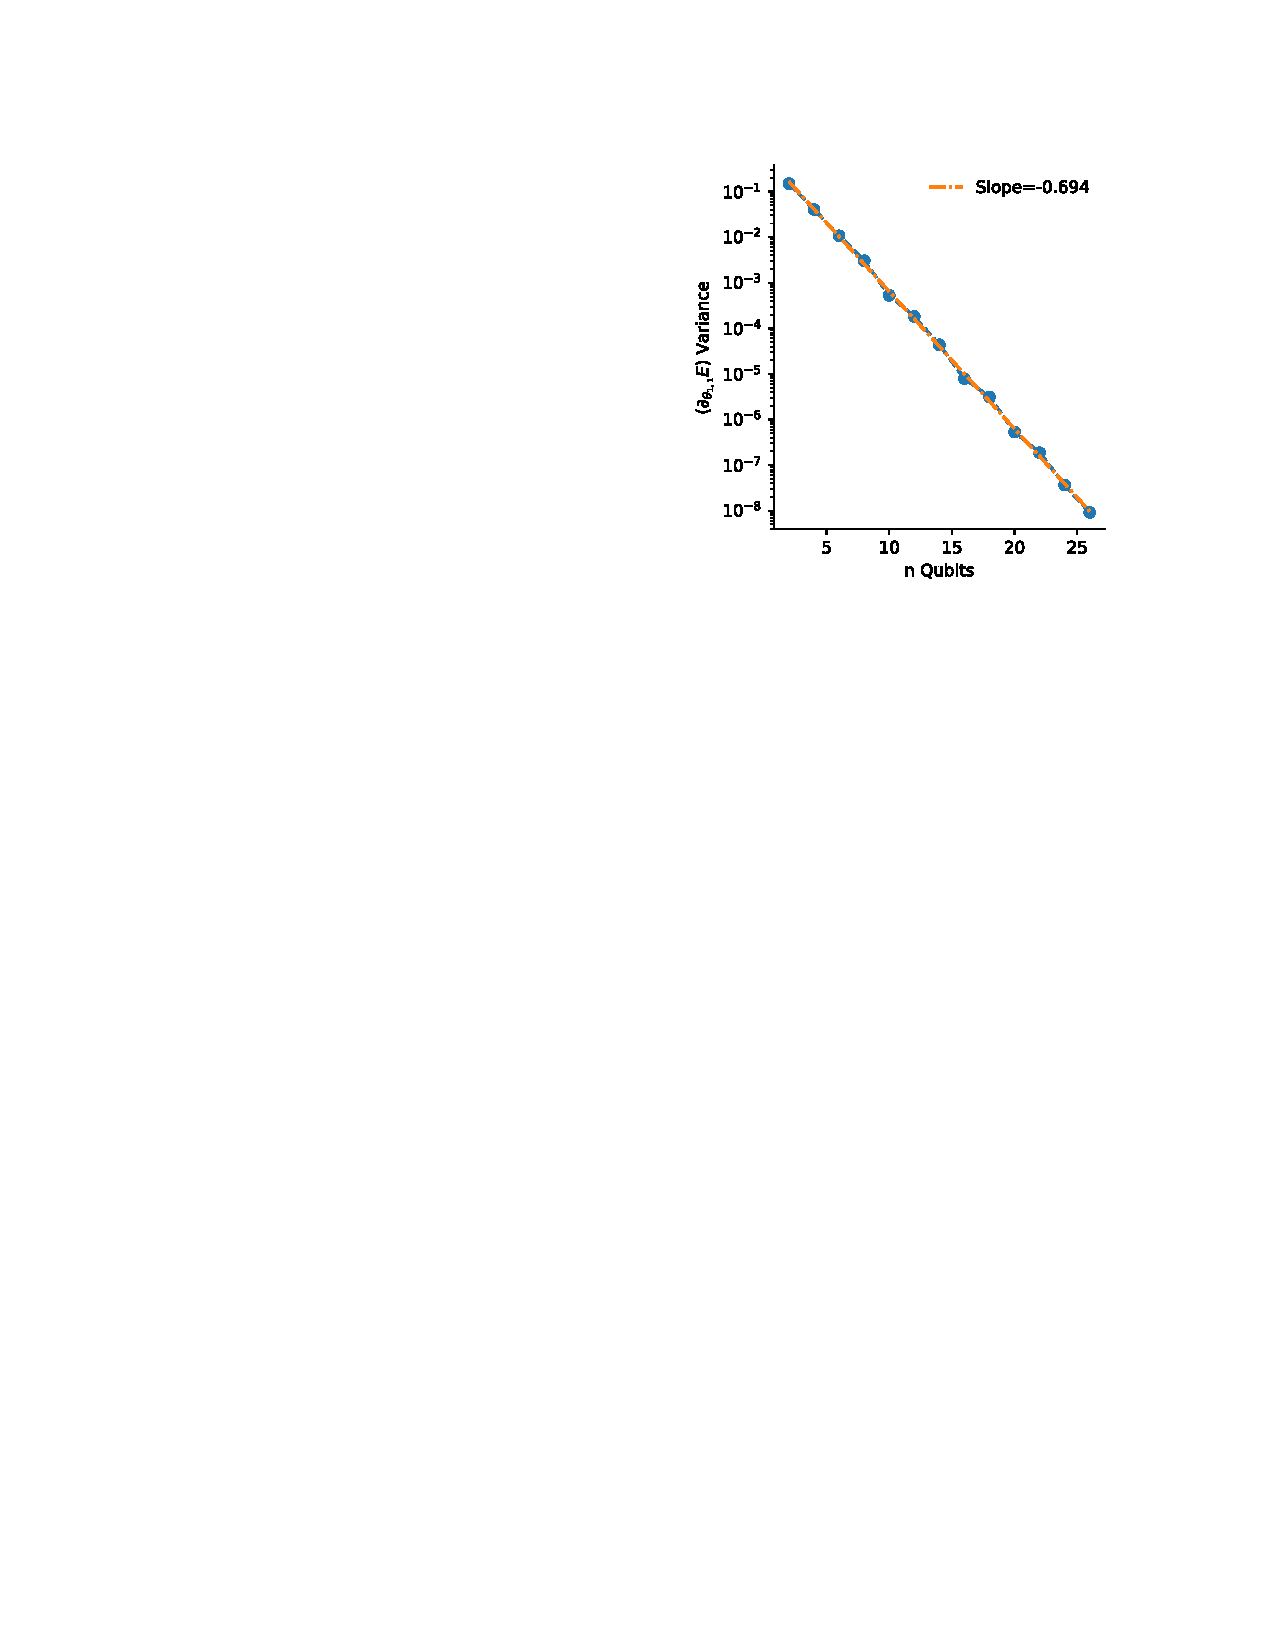
\includegraphics[width=8cm]{bp-var.pdf}
%     \caption{\cite{mcclean2018barren}}
% \end{figure}


\subsection{原因}\label{subsec:bp-cause}
バレンプラトーの原因として既に知られているものを以下に挙げる。
\begin{itemize}
    \item 学習回路の深さ・学習回路の表現能力・学習回路の生成するエンタングルメント~\cite{mcclean2018barren,cerezo2021cost,holmes2022connecting,marrero2021entanglement,leone2022practical}
    \item オブザーバブルの局所性~\cite{cerezo2021cost,uvarov2021barren}
    \item ノイズ~\cite{wang2021noiseinduced}
    \item データの入力~\cite{thanasilp2022exponential,thanasilp2021subtleties,leone2022practical}
\end{itemize}

バレンプラトーは、学習回路がユニタリ $2$--デザイン(\ref{sec:unitary-t-design}~節)という条件を満たすときに起きることが最初に示された~\cite{mcclean2018barren}。具体的な定理と証明については、付録の\ref{sec:bp-proof}~節に記す。
学習回路がユニタリ $2$--デザインを満たすことは、学習回路が深く、高い表現能力を持ち、多くのエンタングルメントを生成することを意味する。

オブザーバブルの局所性とは、測定するオブザーバブルが全量子ビットのうちいくつの量子ビットによって測定されるかを指す。グローバルオブザーバブルとは、全量子ビットの状態によって測定されるオブザーバブルのことであり、例えば、$Z\otn{n}$ である。ローカルオブザーバブルとは、全量子ビット数 $n$ に依存しない $m$ 個の量子ビットよって測定されるオブザーバブルのことである。例えば、$Z\otn{m}$ である。また、ローカルオブザーバブルの線形和もローカルオブザーバブルである。

ここで、量子回路の構造・量子ビット数 $n$・量子回路の層数 $L$・オブザーバブルの局所性がコスト関数の勾配の分散に与える影響を再現したものを示す。量子回路の構造として図~\ref{fig:tpa-hea-circuit}にあるように、Tensor Product Ansatz (TPA) と Hardware Efficient Ansatz (HEA) を用いた。

\begin{figure}[H]
    \centering
    \begin{tikzpicture}
        \node[scale=0.9]{
        \begin{quantikz}
            \lstick{$\ket{0}$}\slice{} & \gate{R_x(\th_{l,1})} & \gate{R_y(\th_{l,5})}\slice{$\times L$}& \meter{}\\
            \lstick{$\ket{0}$}         & \gate{R_x(\th_{l,2})} & \gate{R_y(\th_{l,6})}                & \meter{}\\
            \lstick{$\ket{0}$}         & \gate{R_x(\th_{l,3})} & \gate{R_y(\th_{l,7})}                & \meter{}\\
            \lstick{$\ket{0}$}         & \gate{R_x(\th_{l,4})} & \gate{R_y(\th_{l,8})}                & \meter{}
        \end{quantikz}
        \qquad\qquad
        \begin{quantikz}
            \lstick{$\ket{0}$}\slice{} & \gate{R_x(\th_{l,1})} & \gate{R_y(\th_{l,5})} & \ctrl{1}&  \qw    & \qw\slice{$\times L$}&\meter{}\\
            \lstick{$\ket{0}$}         & \gate{R_x(\th_{l,2})} & \gate{R_y(\th_{l,6})} & \targ{} & \ctrl{1}&\qw                &\meter{}\\
            \lstick{$\ket{0}$}         & \gate{R_x(\th_{l,3})} & \gate{R_y(\th_{l,7})} & \qw     & \targ{} &\ctrl{1}           &\meter{}\\
            \lstick{$\ket{0}$}         & \gate{R_x(\th_{l,4})} & \gate{R_y(\th_{l,8})} & \qw     &   \qw   &\targ{}            &\meter{}
        \end{quantikz}
        };
    \end{tikzpicture}
    \caption{TPA(左)と HEA(右)の量子回路}
    \label{fig:tpa-hea-circuit}
\end{figure}

\begin{figure}[H]
    \begin{minipage}[b]{0.5\columnwidth}
        \centering
        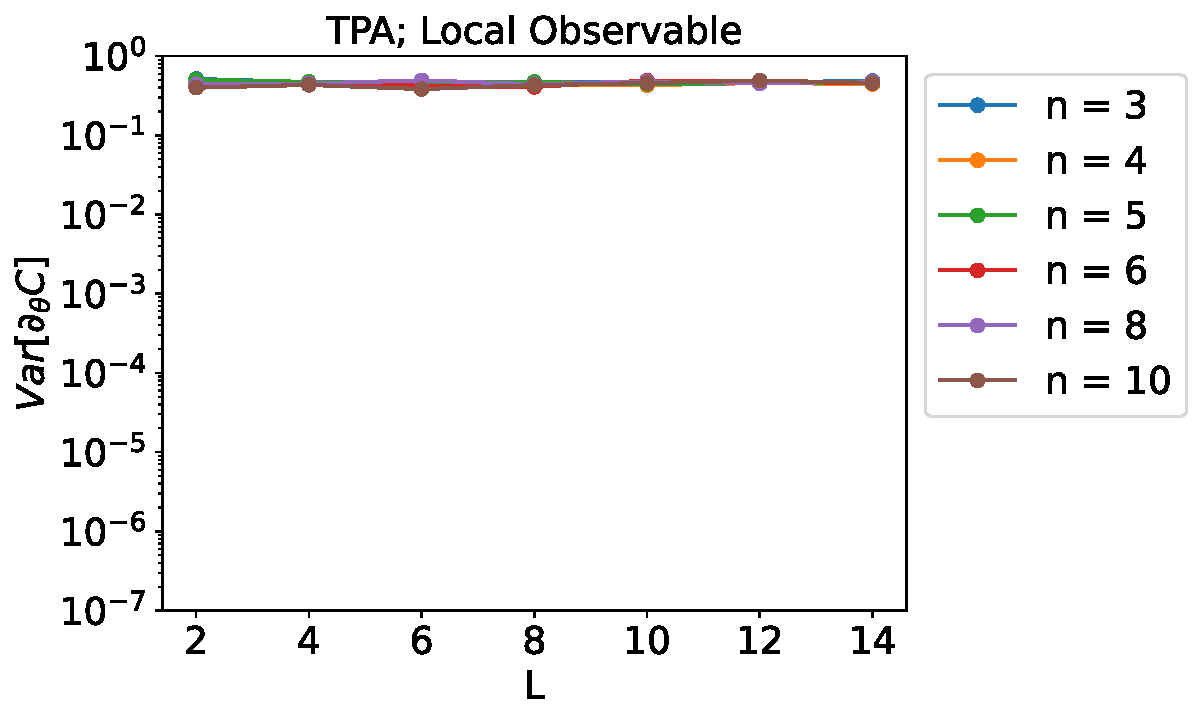
\includegraphics[width=8.5cm]{TPA-local-ob.pdf}
    \end{minipage}
    \hspace{0\columnwidth}
    \begin{minipage}[b]{0.5\columnwidth}
        \centering
        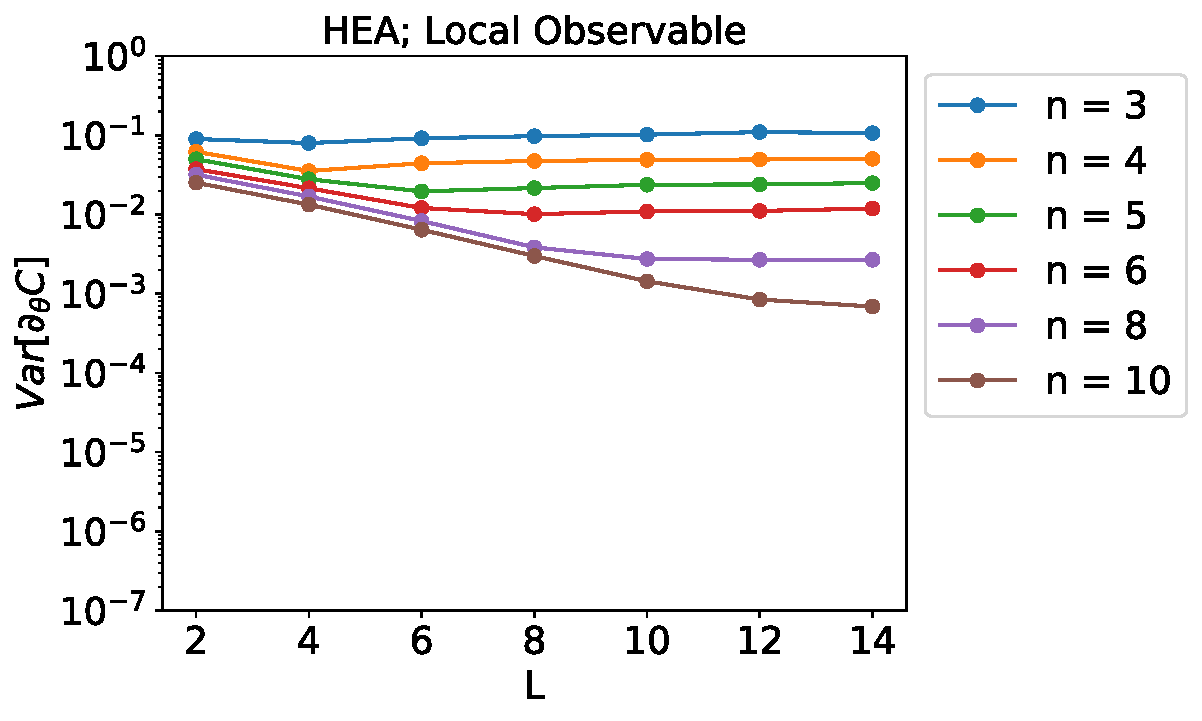
\includegraphics[width=8.5cm]{HEA-local-ob.pdf}
    \end{minipage}
\end{figure}
\begin{figure}[H]
    \begin{minipage}[b]{0.5\columnwidth}
        \centering
        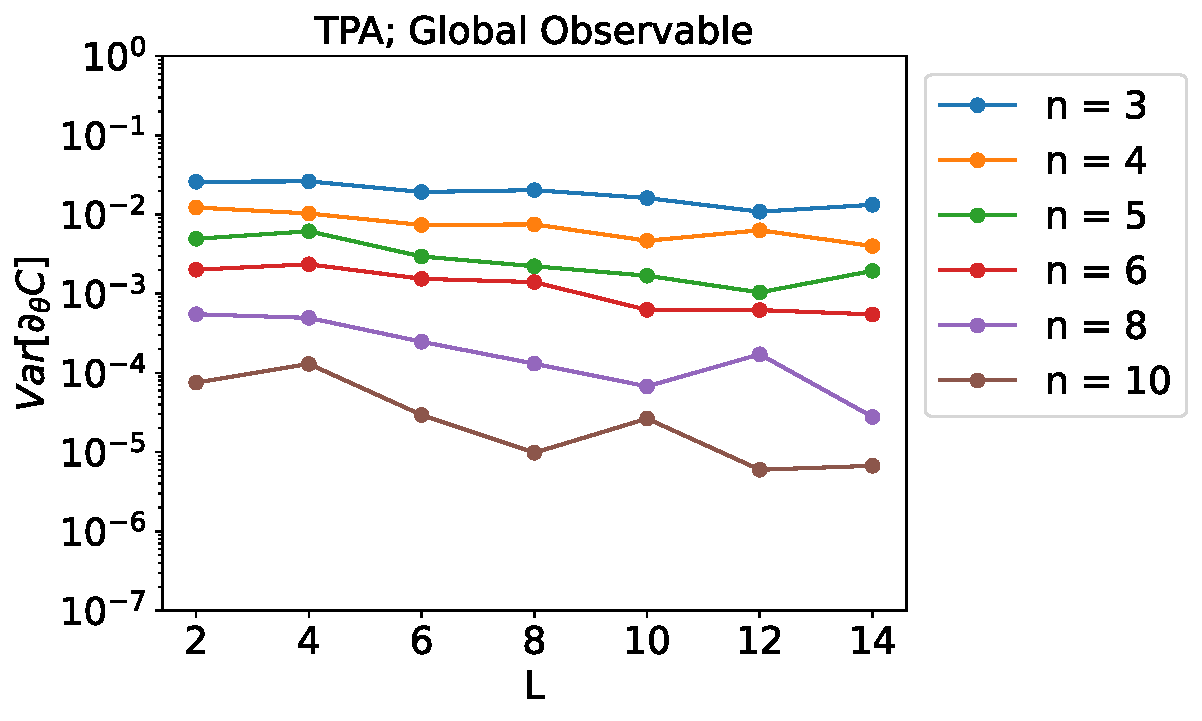
\includegraphics[width=8.5cm,height=5cm]{TPA-global-ob.pdf}
    \end{minipage}
    \hspace{0\columnwidth}
    \begin{minipage}[b]{0.5\columnwidth}
        \centering
        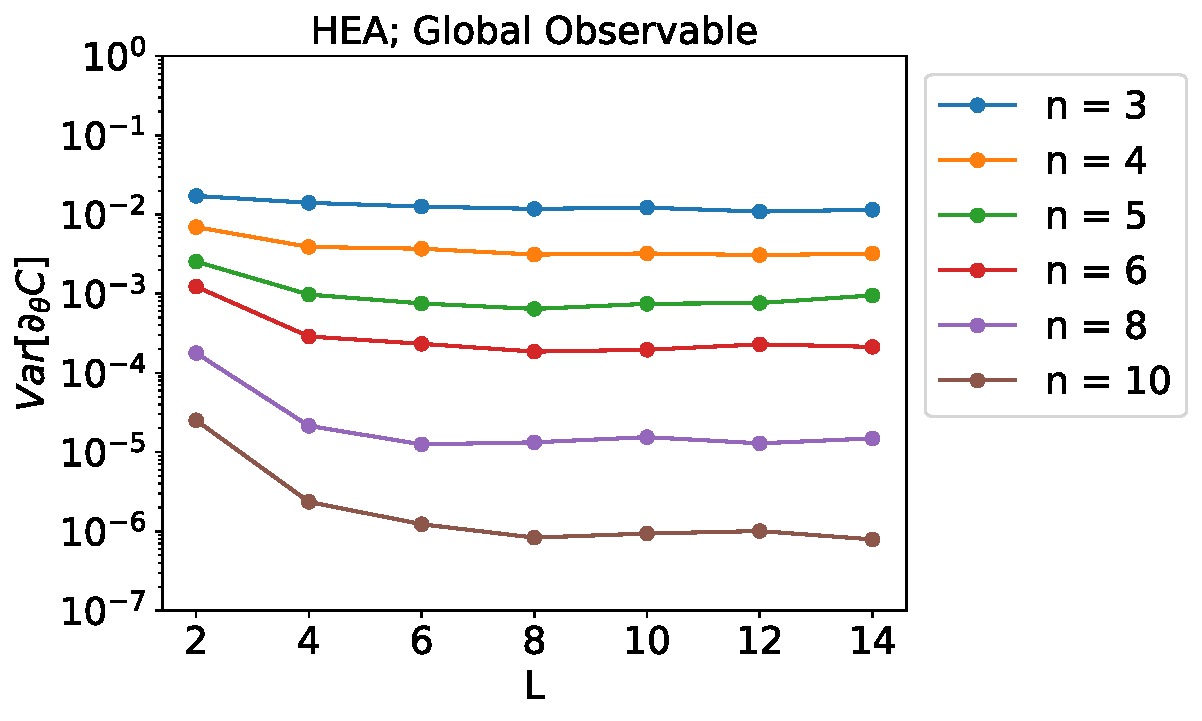
\includegraphics[width=8.5cm,height=5cm]{HEA-global-ob.pdf}
    \end{minipage}
    \caption{それぞれのプロットの横軸は量子回路の各層数 $L$、縦軸はコスト関数の勾配の分散を表す。上段は、TPA(左)と HEA(右)に対してローカルオブザーバブル $Z\ot I \ot\cdots\ot I$ を用いた場合の勾配の分散の変化を示している。下段は、グローバルオブザーバブル $\dyad{0}\otn{n}$ を用いた場合のそれぞれの量子回路における勾配の分散の変化を示している。}
    \label{fig:var-ob}
\end{figure}

図~\ref{fig:var-ob}において、上段は、Tensor Product Ansatz (TPA)(左)と Hardware Efficient Ansatz (HEA)(右)に対してローカルオブザーバブル $Z\ot I \ot\cdots\ot I$ を用いた場合の、各量子ビット数 $n$ と量子回路の各層数 $L$ に対する勾配の分散の変化を示している。下段は、グローバルオブザーバブル $\dyad{0}\otn{n}$ を用いた場合の勾配の分散の変化を示している。これらの図から、エンタングルメントを多く生成すること、層数 $L$ を増やすこと、グローバルオブザーバブルを用いることはいずれも、勾配の分散のスケールをより小さくすることがわかる。


\subsection{回避方法}
豊かな表現能力を持ち、エンタングルメントを多く生成するような深い量子回路を用いることと、グローバルオブザーバブルを用いることは、パラメーターの探索すべき領域を指数関数的に増大させるため、バレンプラトーを引き起こすと考えられている。よって、バレンプラトーを回避するためには、学習回路の深さ・表現能力・エンタングルメントを抑えて、ローカルオブザーバブルを用い、かつ、学習回路の表現領域にコスト関数の最適解があるようにその構造を設計する必要がある。
これらの原因を考慮して、バレンプラトーを回避するための方法がいつくか提案されている。
\begin{itemize}
    \item ローカルオブザーバブルを用いる~\cite{cerezo2021cost}。これにより、データ入力がない場合は、学習回路の深さが $\order{\log{n}}$ であればバレンプラトーは起きないことが示されている。
    \item 学習回路の各層ごとにパラメーターを最適化する~\cite{skolik2021layerwise}。これにより、実質的な学習回路の深さを減らすことができる。
    \item 一部の学習パラメーターの初期値を残りの回路と打ち消し合うように設定する~\cite{grant2019initialization}。これにより、実質的な学習回路の深さを減らすことができる。
    \item 学習パラメーター間に相関を持たせる~\cite{holmes2022connecting}。これにより、学習回路の表現能力を抑えることができる。
    \item 学習パラメーターの初期値を、一様分布ではなく、正規分布からサンプリングする~\cite{zhang2022escaping}。
\end{itemize}

また、QAOA では、最適なパラメーターがあるパターンを持つことが先行研究\cite{zhou2020quantum}で示された。このパターンに近いパラメーターを初期値として用いることで、ランダムにパラメーターを選んだ場合よりも学習が早くなることも示されている。
また、Quantum Tree Tensor Network (QTTN) や Quantum Convolutional Neural Network (QCNN) はその構造上、バレンプラトーが起きないことが示されている\cite{cong2019quantum,martin2022barren}。

しかしながら、バレンプラトーを避けることだけできれば良いわけではない。というのも、例えば、バレンプラトーを避けるためにエンタングルメントが生じない量子回路を用いたとすると、その量子回路は古典コンピューターによって効率的にシミュレーションすることができる。よって、変分量子アルゴリズムにおいて古典計算よりも効率的な計算を行うためには、バレンプラトーを避ける一方で、古典コンピューターによるシミュレーションが困難な量子回路を用いる必要がある。

\newpage
\chapter{ハール分布と量子回路の表現力}\label{chap:haar}
変分量子アルゴリズムにおいては、しばしば、パラメーターの初期値がランダムに選ばれ、それがバレンプラトーと関係することを前章で述べた。ユニタリ群における一様なランダムネスを考える場合、ハール分布やユニタリデザインという概念が重要になる。後の\ref{chap:upper-bound}, \ref{chap:lower-bound}~章の解析においても、これらの概念に基づいて解析を行う。よって、この章においては、ハール分布やユニタリデザインの定義から始め、それらの性質や関連する定理、更に量子回路の表現力と呼ばれる量について説明する。
\ref{sec:haar-random}~節では、ハール分布とそれに関する積分の公式について説明する。
\ref{sec:unitary-t-design}~節でユニタリ $t$--デザインというユニタリの集合に関する性質について説明する。
\ref{sec:expressibility}~節では、量子回路の表現力について説明する。

\section{ハール分布}\label{sec:haar-random}
ハール分布(測度)とはコンパクト群上の一様分布であり、ユニタリ群上のハール分布 $\mu_{\Haar}$ は、ユニタリ群 $\calU(d)$ 上のユニタリ不変な測度であって、以下の性質を満たすものである。
\begin{align}
    \mu_{\Haar}(\calU(d)) = \const,\;\;
    \mu_{\Haar}(g\bbU) = \mu_{\Haar}(\bbU g) = \mu_{\Haar}(\bbU),\,\,\forall g\in \calU(d),\;\;
    \forall \bbU\subset \calU(d)
\end{align}
ここでは確率分布を考えるため $\mu_{\Haar}(\calU(d)) = 1$ とする。
ハールランダムなユニタリ $U$ とは、ハール分布 $\mu_{\Haar}$ からサンプリングされたユニタリ $U$ のことを指す。

$2\times 2$ 次元のハールランダムなユニタリをサンプリングして $\ket{0}$ に作用させると、それらの状態は、図~\ref{fig:haar-1qubit}のようにブロッホ球面上で一様に分布する。
\begin{figure}[H]
    \centering
    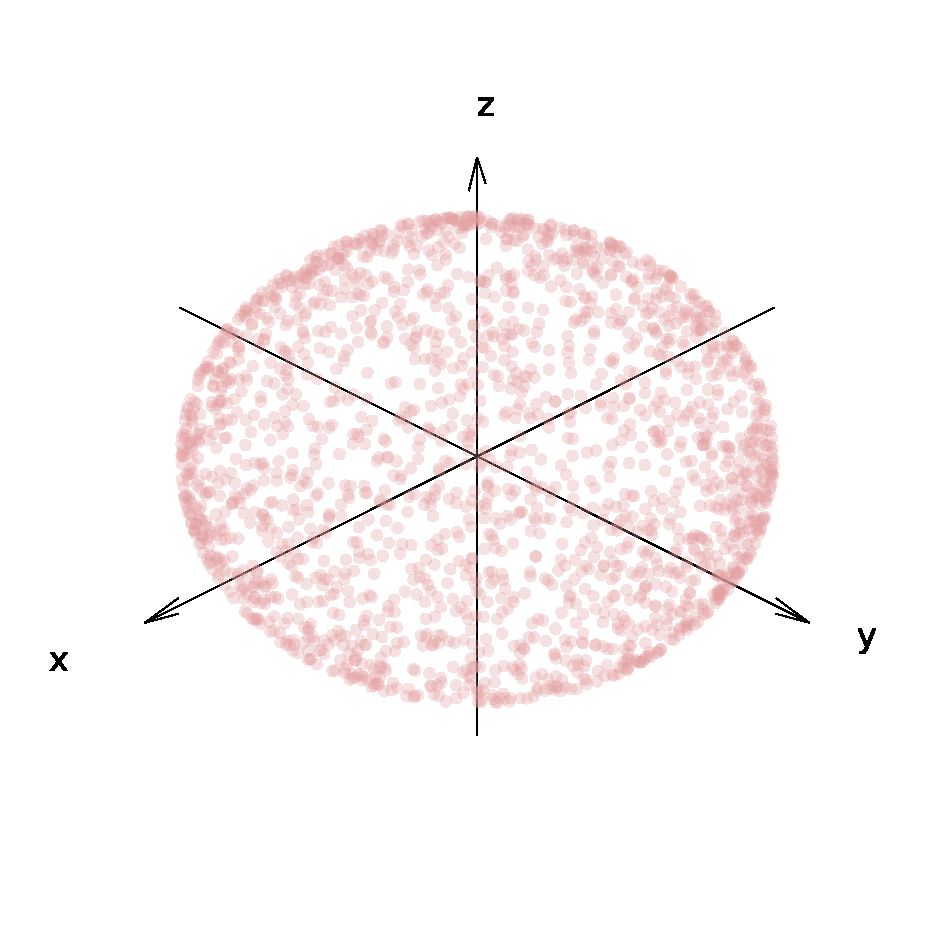
\includegraphics[width=10cm]{haar-sampling.pdf}
    \caption{ブロッホ球面上でのハール分布}
    \label{fig:haar-1qubit}
\end{figure}

% \subsection{ハール分布の積分公式}
ユニタリ群上のハール分布においては、次のような積分公式が成り立つ。
\begin{screen}
    \begin{theorem}
        ハール分布に従うユニタリ $W$ に関する積分は以下のように計算できる。
        \begin{align}
            \int_{\calU(d)} d\mu_{\Haar}(W)\, w_{\bs{i},\bs{j}}
            w_{\bs{p},\bs{q}}^*
            &= \frac{\delta_{\bs{i},\bs{p}}\delta_{\bs{j},\bs{q}}}{d} \label{eq:haar-int-1}\\
            % 
            \int_{\calU(d)} d\mu_{\Haar}(W)\, w_{\bs{i}_1,\bs{j}_1}
            w_{\bs{i}_2,\bs{j}_2}
            w_{\bs{i}_1^\prime,\bs{j}_1^\prime}^*
            w_{\bs{i}_2^\prime,\bs{j}_2^\prime}^*
            &= \frac{1}{d^2-1}
            (\delta_{\bs{i}_1,\bs{i}_1^\prime}\delta_{\bs{i}_2,\bs{i}_2^\prime}
            \delta_{\bs{j}_1,\bs{j}_1^\prime}\delta_{\bs{j}_2,\bs{j}_2^\prime}
            +\delta_{\bs{i}_1,\bs{i}_2^\prime}\delta_{\bs{i}_2,\bs{i}_1^\prime}
            \delta_{\bs{j}_1,\bs{j}_2^\prime}\delta_{\bs{j}_2,\bs{j}_1^\prime}) \nonumber\\
            &- \frac{1}{d(d^2-1)}
            (\delta_{\bs{i}_1,\bs{i}_1^\prime}\delta_{\bs{i}_2,\bs{i}_2^\prime}
            \delta_{\bs{j}_1,\bs{j}_2^\prime}\delta_{\bs{j}_2,\bs{j}_1^\prime}
            +\delta_{\bs{i}_1,\bs{i}_2^\prime}\delta_{\bs{i}_2,\bs{i}_1^\prime}
            \delta_{\bs{j}_1,\bs{j}_1^\prime}\delta_{\bs{j}_2,\bs{j}_2^\prime}) \label{eq:haar-int-2}
        \end{align}
    \end{theorem}
\end{screen}

たとえば、公式~\eqref{eq:haar-int-1} を用いると、次のような積分を計算することができる。
\begin{align}
    \int_{\calU(d)} d\mu_{\Haar}(W)\, |\ev{W}{\bs{0}}|^2
    &= \int_{\calU(d)} d\mu_{\Haar}(W)\, w_{\bs{0},\bs{0}}\,w_{\bs{0},\bs{0}}^*
    = \frac{1}{d}
\end{align}

さらに、公式~\eqref{eq:haar-int-2} を用いることで、次の公式を導くことができる。
\begin{align}\label{eq:haar-int-5}
    \int_{\calU(d)} d\mu_{\Haar}(W)\, \Tr[WAW\dg B]\Tr[WCW\dg D]
    &= \frac{1}{d^2-1}
    (\Tr[A]\Tr[B]\Tr[C]\Tr[D] + \Tr[AC]\Tr[BD]) \nonumber\\
    &- \frac{1}{d(d^2-1)}
    (\Tr[AC]\Tr[B]\Tr[D] + \Tr[A]\Tr[C]\Tr[BD])
\end{align}
\begin{align}\label{eq:haar-int-6}
    \int_{\calU(d)} d\mu_{\Haar}(W)\, \Tr[AW\otn{2}B(W\dg)\otn{2}]
    &= \frac{1}{d^2-1}(\Tr[A]\Tr[B] + \Tr[A\,\SWAP]\Tr[B\,\SWAP]) \nonumber\\
    &- \frac{1}{d(d^2-1)}(\Tr[A\,\SWAP]\Tr[B] + \Tr[A]\Tr[B\,\SWAP])
\end{align}
ただし、$\SWAP = \sum_{i,j=1}^d \ket{ij}\bra{ji}$ である。証明は、論文~\cite{cerezo2021cost}の Supplementary Note 1 を参照。


これらの公式とテンソルネットワークによる記法を組み合わせることで、ハール分布に関する積分を行列の脚の繋ぎ替えたものの和として表現することができる。テンソルネットワークとは、大きな量子状態を効率的に表現するための方法である。以下に、必要なテンソルネットワークの記法を示す。

\begin{figure}[H]
    \centering
    \begin{tikzpicture}[scale=1]
        % Vector
        % Define the nodes
        \node[draw, rectangle] (v) at (0,0) {{\LARGE $v$}};
        % Connect the nodes
        \draw (v) -- (-2, 0) node[left] {$i$};
        
        % Matrix
        % Define the nodes
        \node[draw, rectangle] (A) at (4,0) {{\LARGE $A$}};
        % Connect the nodes
        \draw (A) -- (2, 0) node[left] {$j$};
        \draw (A) -- (6, 0) node[right] {$k$};
    \end{tikzpicture}
    \caption{べクトルと行列}
\end{figure}

\begin{figure}[H]
    \centering
    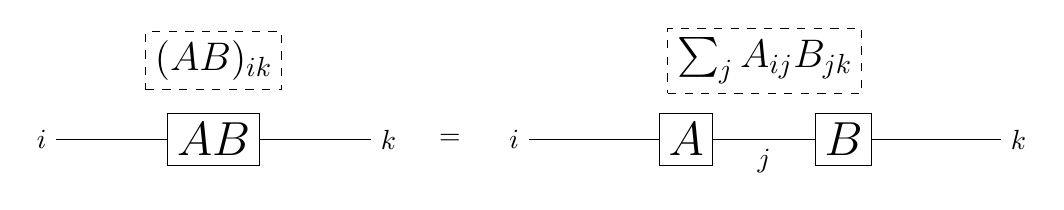
\begin{tikzpicture}[scale=1]
        % Define the nodes
        \node[draw,rectangle]        (AB)  at (-4,0) {{\LARGE $AB$}};
        \node[draw,rectangle,dashed] (eq1) at (-4,1) {{\Large $(AB)_{ik}$}};
        \node[draw,rectangle]        (A)   at (2,0) {{\LARGE $A$}};
        \node[draw,rectangle]        (B)   at (4,0) {{\LARGE $B$}};
        \node[draw,rectangle,dashed] (eq2) at (3,1) {{\Large $\sum_j A_{ij}B_{jk}$}};
        % Connect the nodes
        \draw (AB) -- (-6, 0) node[left] {$i$};
        \draw (AB) -- (-2,0) node[right] {$k$};
        \draw (-1,0) node {$=$};
        \draw (A) -- (0, 0) node[left] {$i$};
        \draw (A) -- (B) node[midway, below] {$j$};
        \draw (B) -- (6, 0) node[right] {$k$};
    \end{tikzpicture}
    \caption{行列の積}
\end{figure}


\begin{figure}[H]
    \centering
    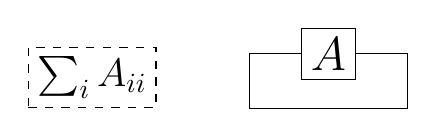
\begin{tikzpicture}[scale=1]
        % Define the nodes for trace
        \node[draw,rectangle]        (A)  at (0,0) {{\LARGE $A$}};
        \node[draw,rectangle,dashed] (eq3) at (-3,-0.3) {{\Large $\sum_i A_{ii}$}};
        % Connect the nodes for trace
        \draw (A.west) -- (-1,0) -- (-1,-0.7) -- (1,-0.7) -- (1,0) -- (A.east);
    \end{tikzpicture}
    \caption{トレース}
\end{figure}

\begin{comment}
\begin{figure}[H]
    \centering
    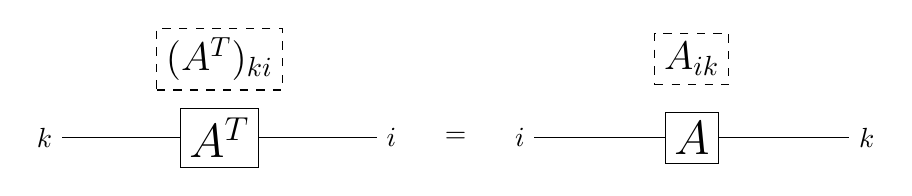
\begin{tikzpicture}[scale=1]
        % Define the nodes for transpose
        \node[draw,rectangle]        (AT)  at (-4,0) {{\LARGE $A^T$}};
        \node[draw,rectangle,dashed] (eq1) at (-4,1) {{\Large $(A^T)_{ki}$}};
        \node[draw,rectangle]        (A)   at (2,0) {{\LARGE $A$}};
        \node[draw,rectangle,dashed] (eq2) at (2,1) {{\Large $A_{ik}$}};
        % Connect the nodes for transpose
        \draw (AT) -- (-6, 0) node[left] {$k$};
        \draw (AT) -- (-2,0) node[right] {$i$};
        \draw (-1,0) node {$=$};
        \draw (A) -- (0, 0) node[left] {$i$};
        \draw (A) -- (4,0) node[right] {$k$};
    \end{tikzpicture}
    \caption{行列の転置}
\end{figure}

\begin{figure}[H]
    \centering
    \includegraphics[width=10cm]{tensor-mat@vec.png}
    \caption{}
\end{figure}

\begin{figure}[H]
    \centering
    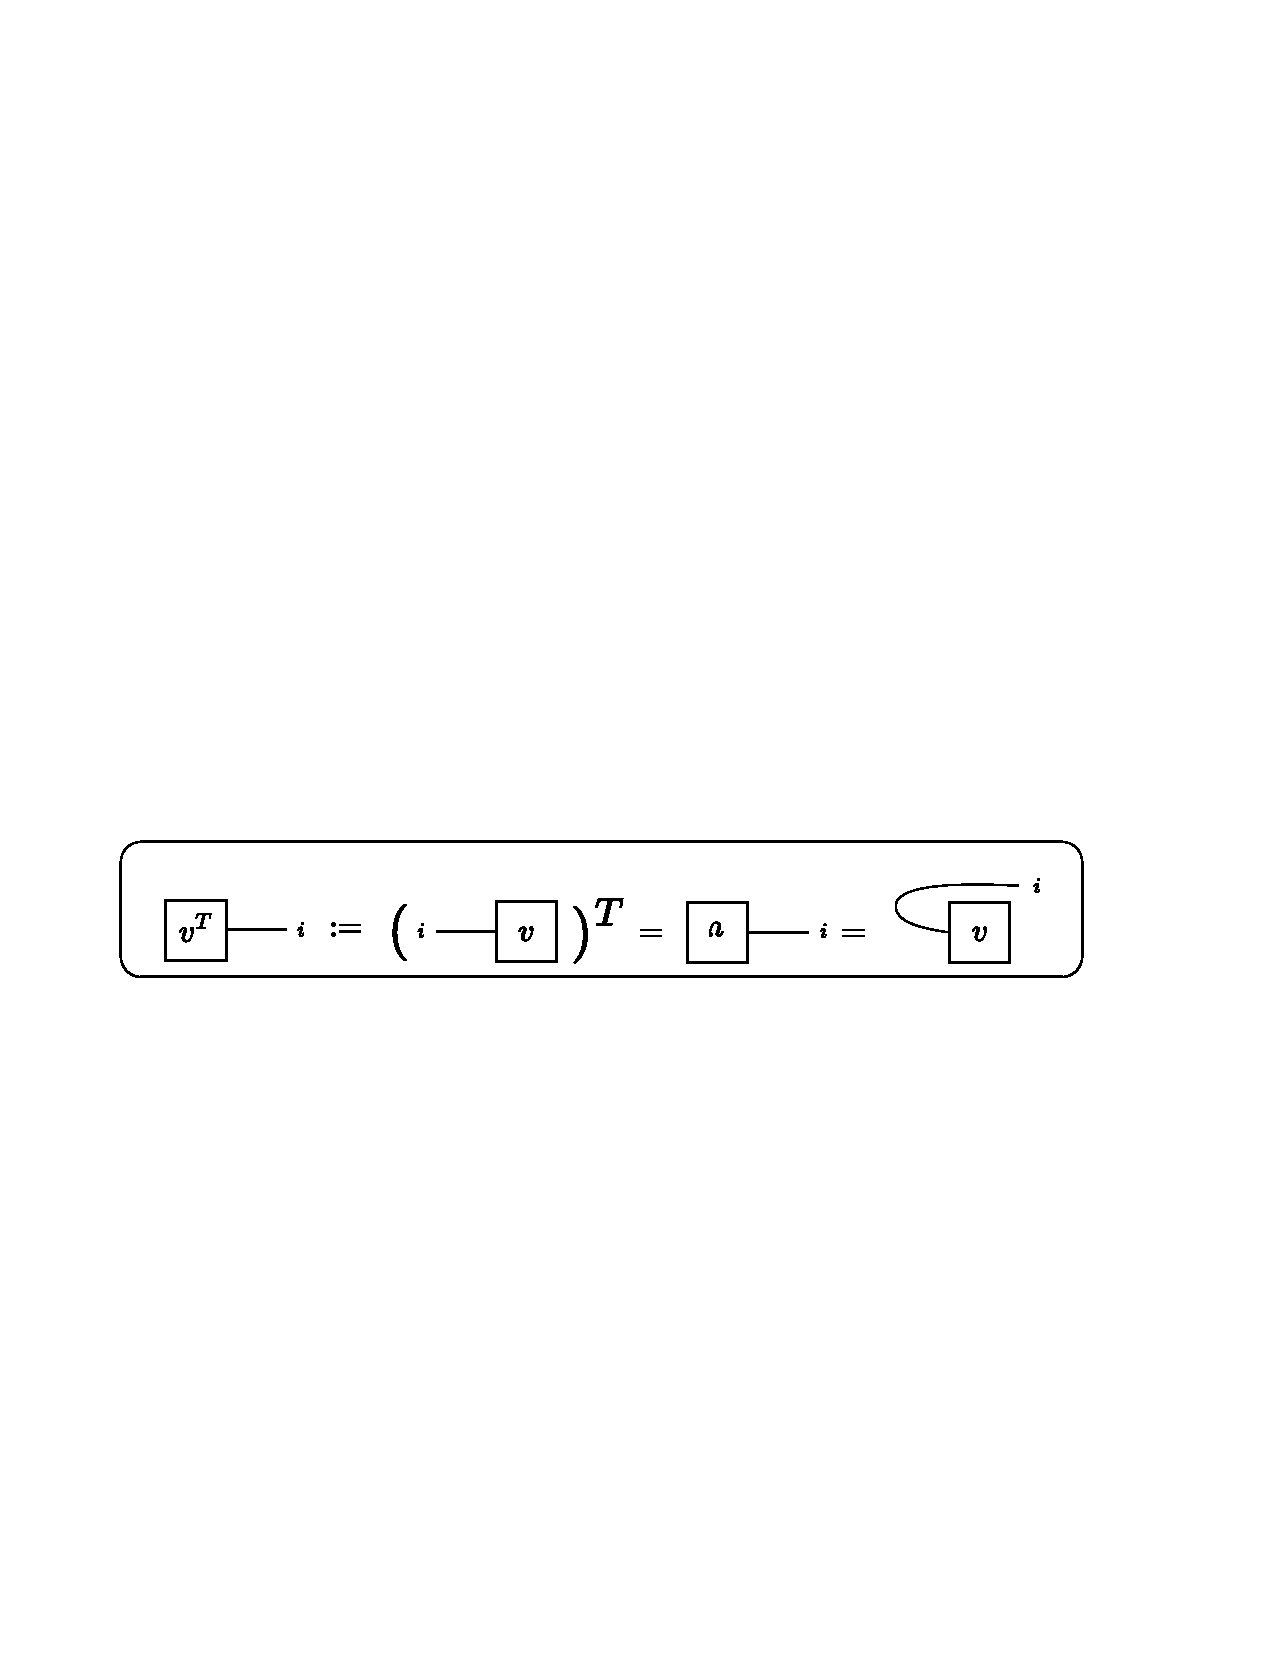
\includegraphics[width=14cm]{tensor-vec-t.png}
    \caption{}
\end{figure}

\begin{figure}[H]
    \centering
    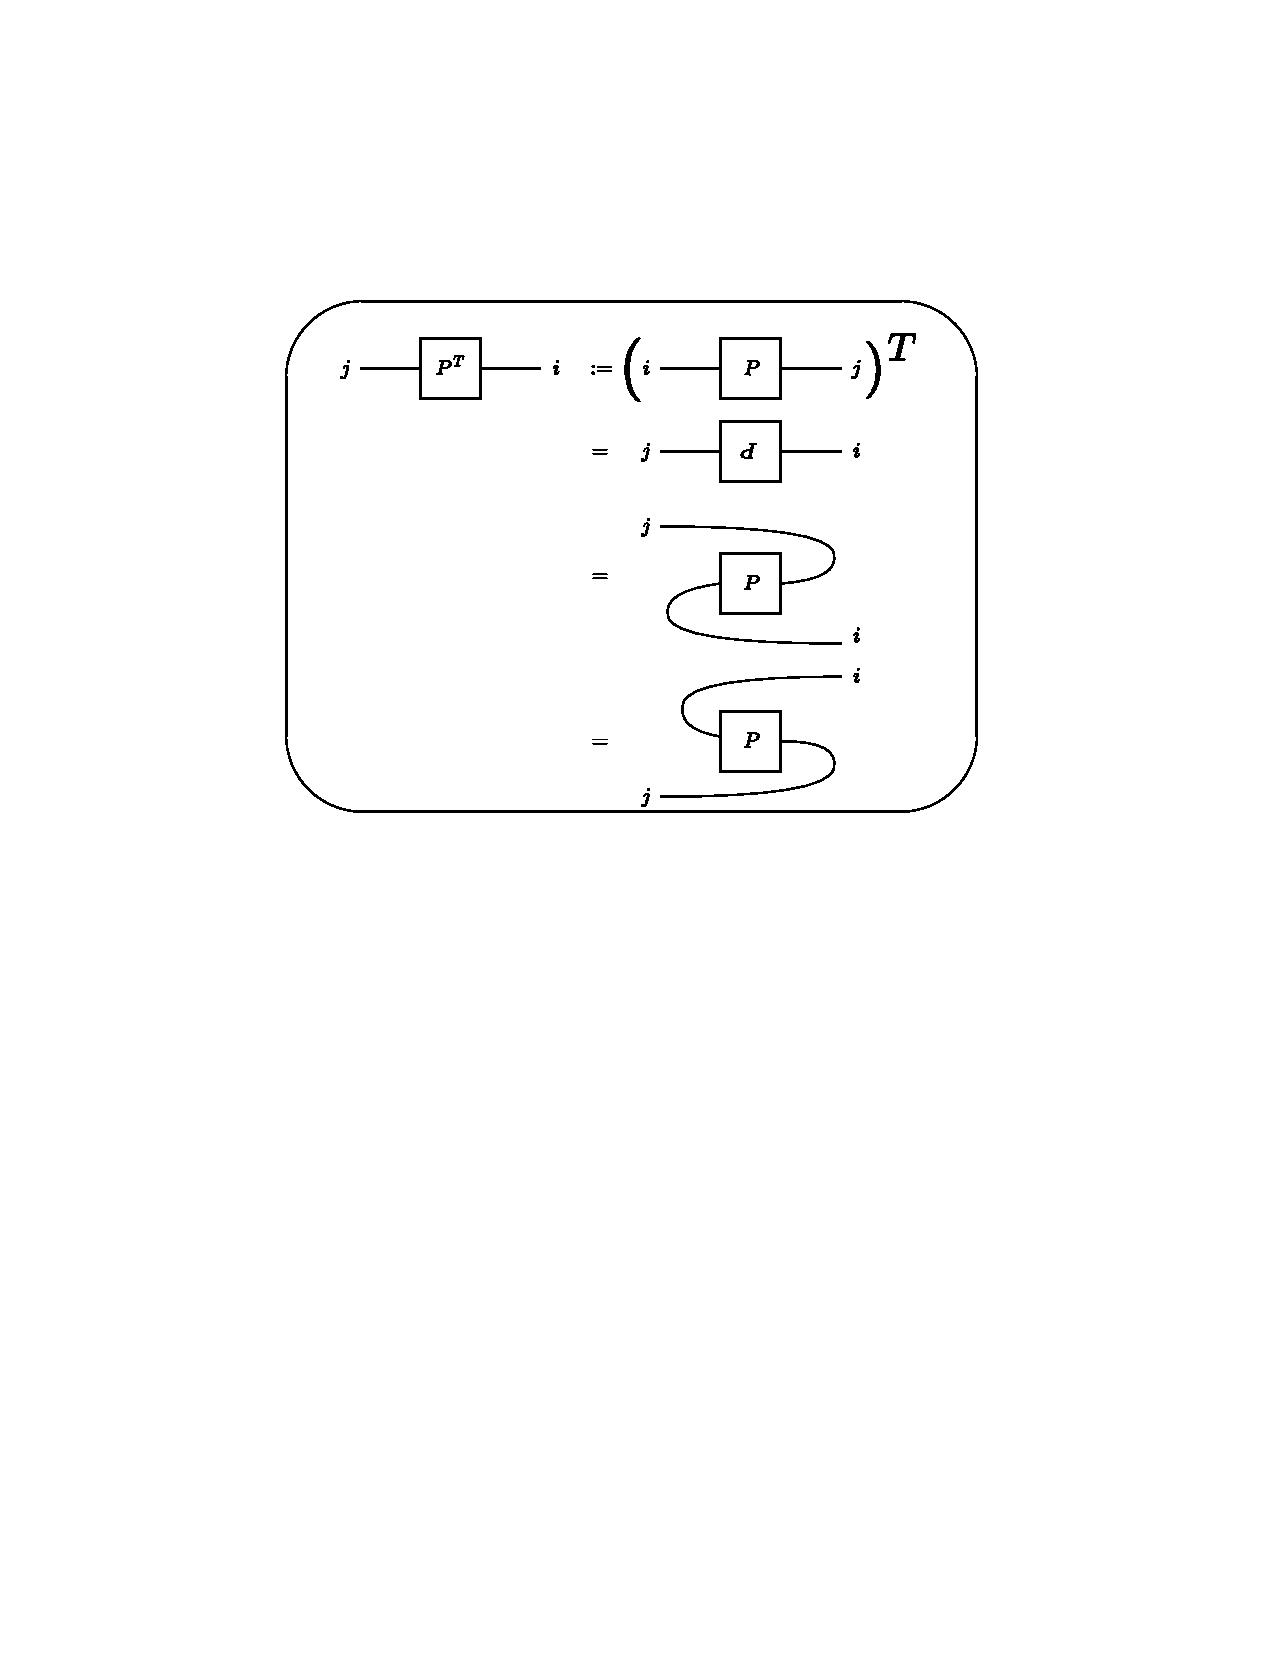
\includegraphics[width=10cm]{tensor-mat-t.png}
    \caption{}
\end{figure}
\end{comment}


例えば、公式~\eqref{eq:haar-int-1}を用いて、次の積分公式を示せる。
\begin{align}\label{eq:haar-int-3}
    \int_{\calU(d)} d\mu_{\Haar}(U)\; AUBU\dg C = \frac{\Tr[B]AC}{d}
\end{align}
テンソルネットワークによる記法を用いると、図~\ref{fig:haar-int-3}のように表現することができる。

\begin{figure}[H]
    \centering
    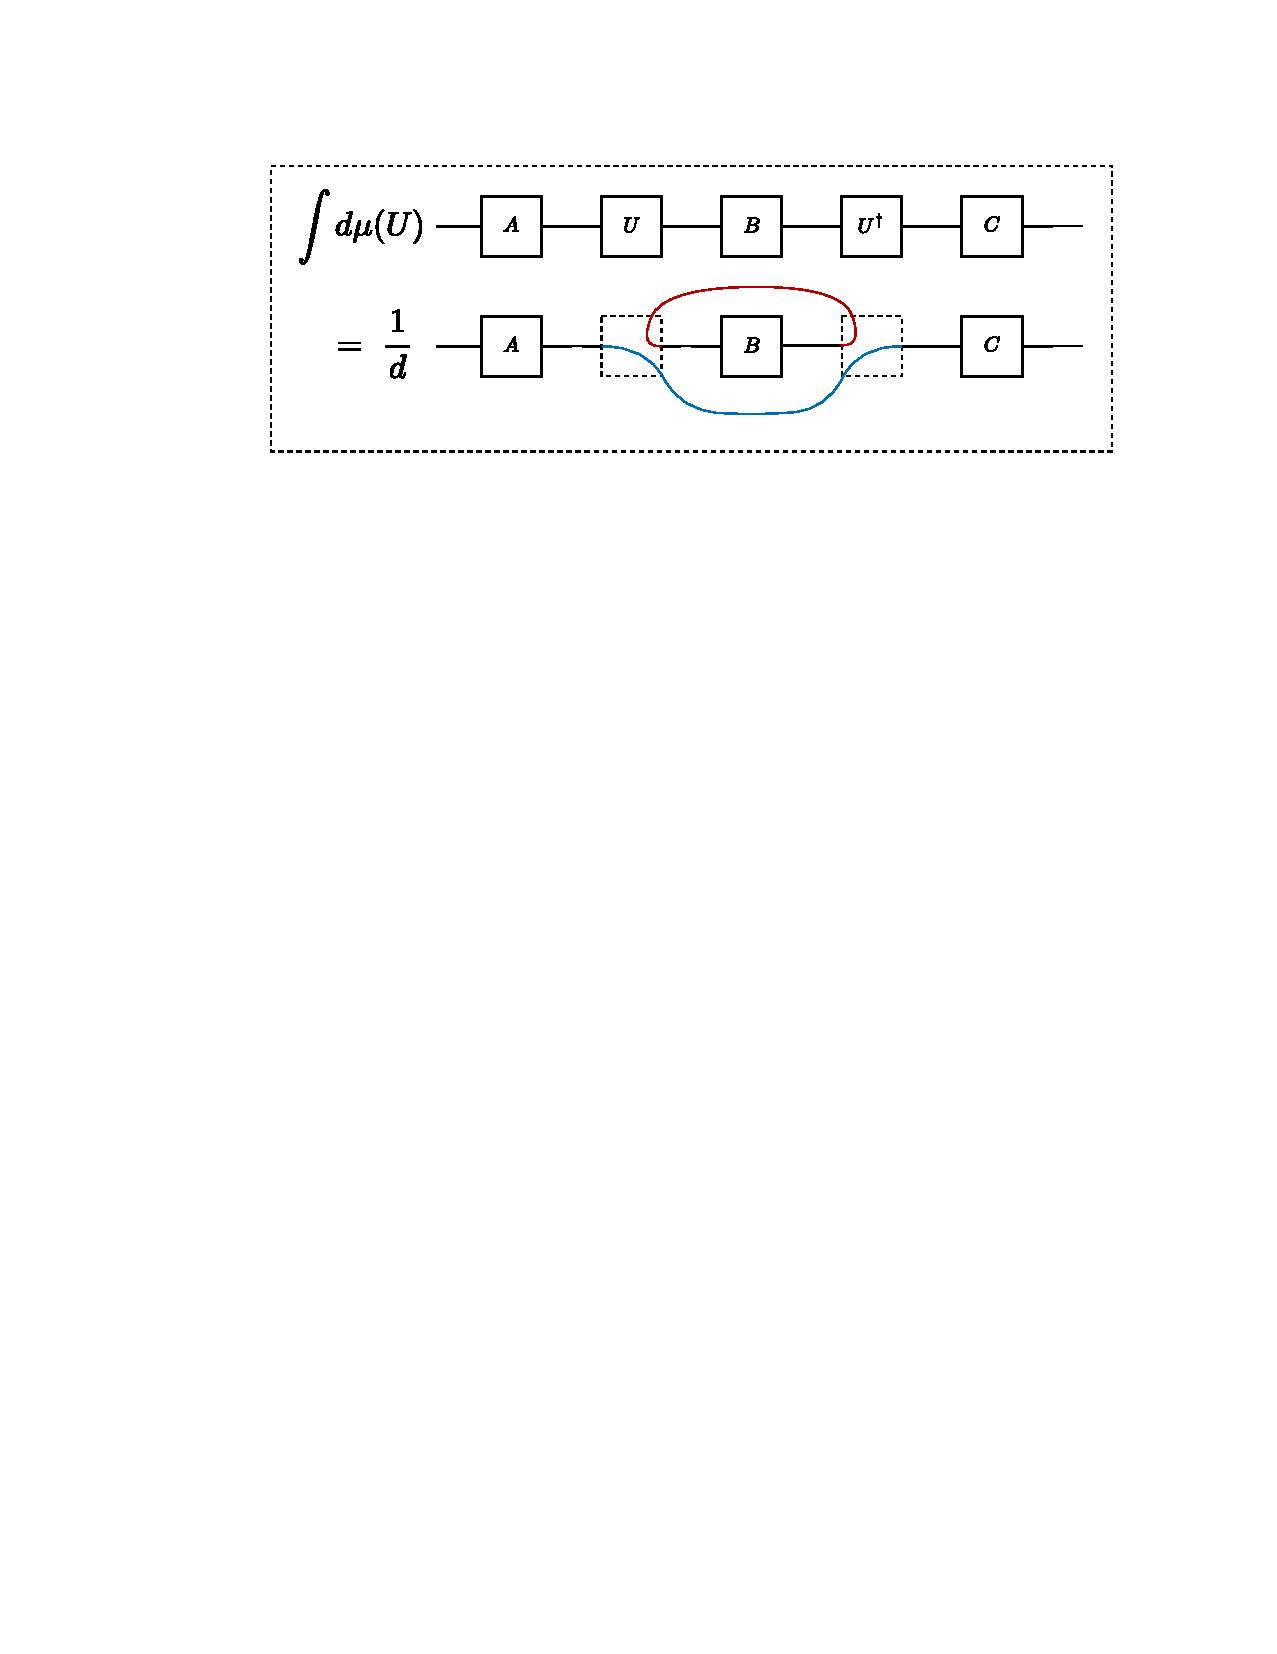
\includegraphics[width=14cm]{haar-int.pdf}
    \caption{公式~\eqref{eq:haar-int-3}に対応するテンソルネットワーク}
    \label{fig:haar-int-3}
\end{figure}

また、公式~\eqref{eq:haar-int-2}を用いて、次の積分公式を示せる。
\begin{align}\label{eq:haar-int-4}
    \int_{\calU(d)} d\mu_{\Haar}(U)\;AUBU\dg CUDU\dg E &= \frac{1}{d^2-1}(\Tr[B]\Tr[D]ACE + \Tr[BD]\Tr[C]AE) \nonumber\\
    &\quad - \frac{1}{d(d^2-1)}(\Tr[BD]ACE + \Tr[B]\Tr[C]\Tr[D]AE)
\end{align}
テンソルネットワークによる記法を用いると、図~\ref{fig:haar-int-4}のように表現することができる。

\begin{figure}[H]
    \centering
    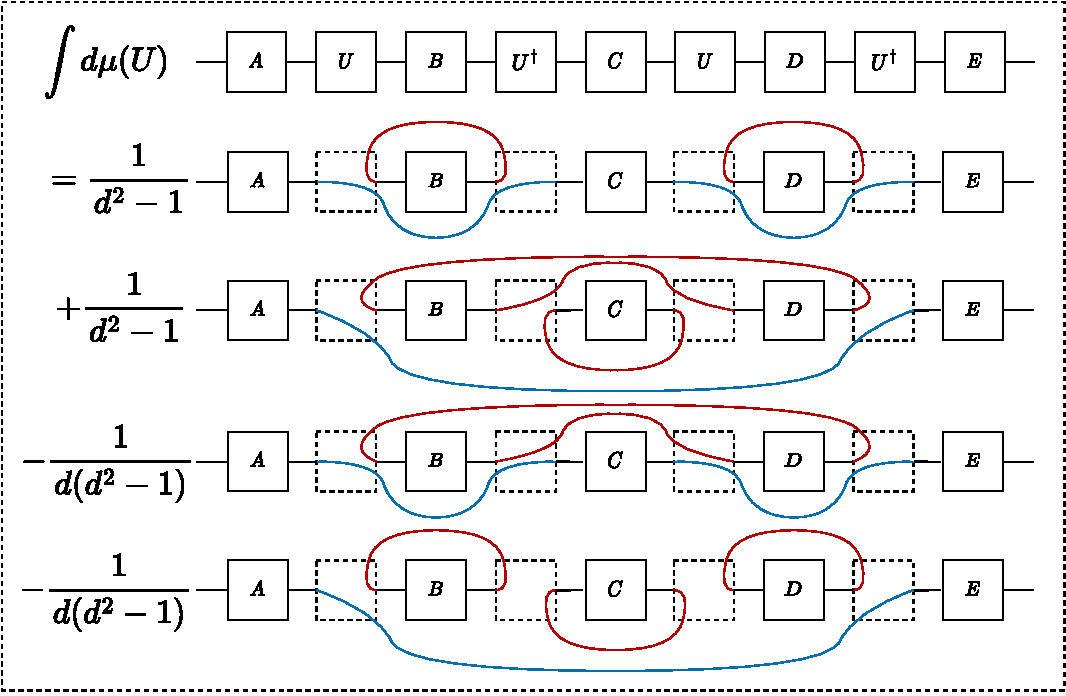
\includegraphics[width=14cm]{haar-int-2.pdf}
    \caption{公式~\eqref{eq:haar-int-4}に対応するテンソルネットワーク}
    \label{fig:haar-int-4}
\end{figure}


% \begin{align}
%     \int_{\calU(d)} d\mu_{\Haar}(W)\, 
%     \Tr[WAW\dg B]
%     &= \frac{\Tr[A]\Tr[B]}{d}
% \end{align}

% \begin{align}
%     \int_{\calU(d)} d\mu_{\Haar}(W)\, \Tr[WAW\dg BWCW\dg D]
%     &= \frac{1}{d^2-1}
%     (\Tr[A]\Tr[C]\Tr[BD] + \Tr[AC]\Tr[B]\Tr[D]) \nonumber\\
%     &- \frac{1}{d(d^2-1)}
%     (\Tr[AC]\Tr[BD] + \Tr[A]\Tr[B]\Tr[C]\Tr[D])
% \end{align}



\section{ユニタリ $t$--デザイン}\label{sec:unitary-t-design}
ユニタリ $t$--デザインとは、ユニタリの集合に関する性質の一つであり、次のように定義される。
\begin{screen}
    \begin{definition}
        $P_{t,t}(U)$ は、ユニタリ $U$ と $U\dg$ のそれぞれの成分に関して最大次数 $t$ の斉次多項式とする。$K$ 個のユニタリの集合 $\{U_k\}$ が以下の条件を満たすとき、この集合はユニタリ $t$--デザインを成すという。
        \begin{align}
            \frac{1}{K} \sum_{k=1}^{K} P_{t,t}(U_k) = \int_{\calU(d)} P_{t,t} (U) d\mu_{\Haar}(U)
        \end{align}
        ここで、$d\mu_{\Haar}$ はハール分布である。
    \end{definition}
\end{screen}
すなわち、ユニタリ $t$--デザインとは、ユニタリの集合に関する斉次多項式 $P_{t,t}(U)$ の平均値が、ユニタリ群上のハール分布に関する積分と厳密に等しいような性質のことである。
ユニタリ $t$--デザインの性質を持つユニタリの集合は、ユニタリ群上において一様に分布した要素の集合である。このような性質を持つユニタリの集合を構成することができれば、ある斉次多項式 $P_{t,t}(U)$ のハール分布に関する積分を、有限のユニタリの集合による平均値として計算することができる。また、$\{U_k\}$ がユニタリ $t$--デザインであれば、$\{U_k\}$ はユニタリ $(t-1)$--デザインでもあることが知られている。

例えば、ユニタリ $t$--デザインの集合として以下のものがある。
\begin{itemize}
    \item Pauli 群 $\calP(n)=\{e^{i\frac{k\pi}{2}}\, P_{j_1}\ot P_{j_2}\ot \cdots\ot P_{j_n}|\;k,j_l=0,1,2,3\}$ はユニタリ $1$--デザインである。
    \item Clifford 群 $\calC(n)=\{U\in \calU(2^n)|\,U\calP(n)U\dg = \calP(n)\}$ はユニタリ $3$--デザインである。
    % $n=1$ のとき、$H \in \calC(1)$ である。なぜなら、$H\bbid H=\bbid,\,HXH=Z,\,HYH=-Y,\,HZH=X$ だからである。
\end{itemize}

図~\ref{fig:design}は、$2\times2$ のユニタリ $1$--デザインとユニタリ $2$--デザインを成す集合を3次元球内の点として表現したものである\cite{gross2007evenly}。

次に言葉の定義を行う。$n$ 量子ビットの系を考えるとする。$2^n \times 2^n$ のユニタリの集合がユニタリ $t$--デザインを成すとき、このことを、考えている系に対してグローバルユニタリ $t$--デザインを成すという。$n$ より小さい自然数 $s$ に対して、$2^s \times 2^s$ のユニタリの集合がユニタリ $t$--デザインを成すとき、このことを、考えている系に対してローカルユニタリ $t$--デザインを成すという。

\begin{figure}[H]
    \begin{minipage}[b]{0.5\columnwidth}
        \centering
        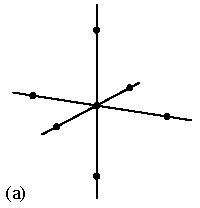
\includegraphics[width=7cm]{1-design.pdf}
    \end{minipage}
    \hspace{0\columnwidth}
    \begin{minipage}[b]{0.5\columnwidth}
        \centering
        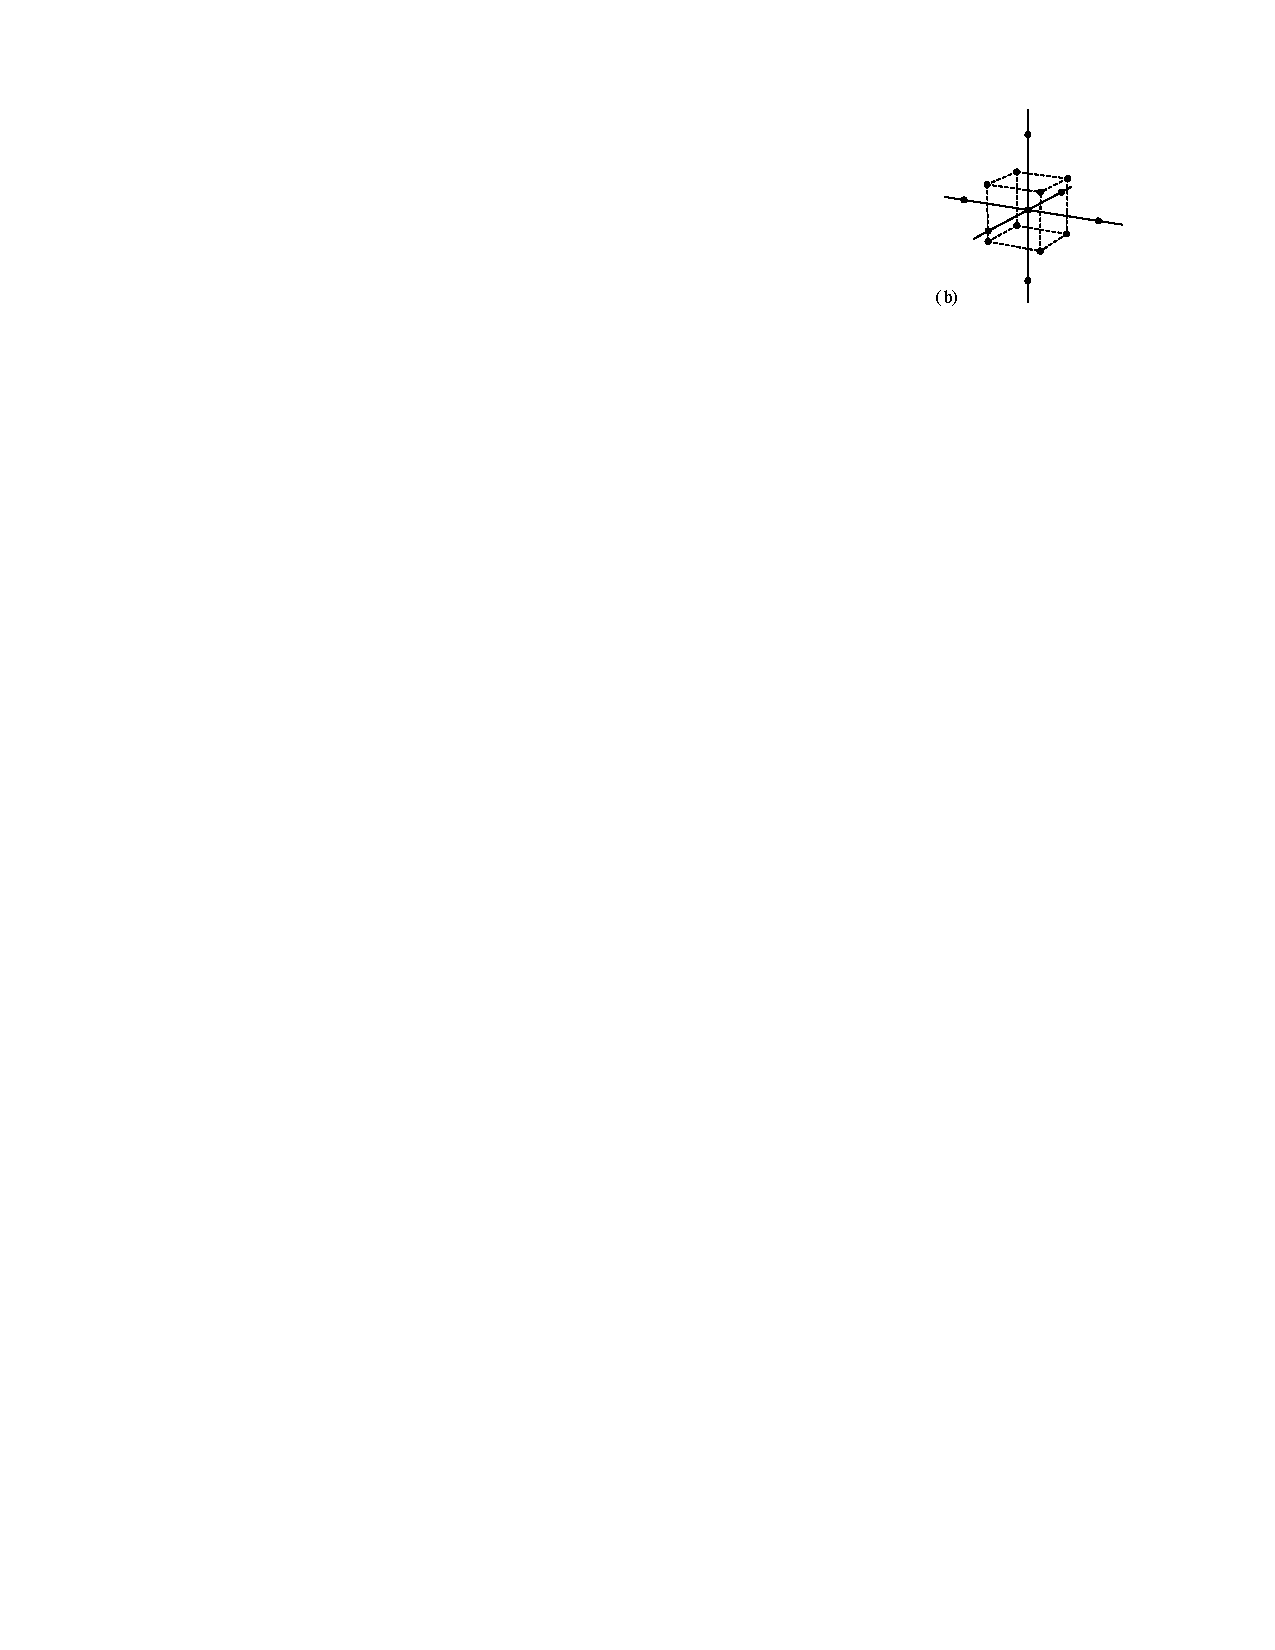
\includegraphics[width=7cm]{2-design.pdf}
    \end{minipage}
    \caption{$SU(2) \sim SO(3)$ なので、$2\times2$ のユニタリは位相を除いて3次元回転に対応する。更に、単位ベクトル $\hat{n}$ 周りの角度 $\varphi \in [0,\pi] $ の回転をベクトル $\varphi\hat{n} \in \bbR^3$ と対応させると、$SO(3)$ は半径 $\pi$ の球内の点として表現できる。左がユニタリ $1$--デザイン、右がユニタリ $2$--デザインの点の集合を表している。ただし、球面の反対側の点は同一視される。論文~\cite{gross2007evenly}より引用}
    \label{fig:design}
\end{figure}


\section{表現力}\label{sec:expressibility}
量子回路によって生成されるユニタリの集合を $\bbU$ と表す。
量子回路の表現力とは、量子回路がどれだけの多くのユニタリを表現できるかという能力(表現能力)を定量化したものであり、次のように定義される。
\begin{screen}
    \begin{definition}\label{def:expressibility}
        量子回路 $\bbU$ の表現力は、次のように定義される。
        \begin{align}
            \epsilon_{\bbU}^{(t,p)}(X) &:= \norm{A_{\bbU}^{(t)}(X)}_p,\\
            \calA_{\bbU}^{(t)}(X) &:= \int_{V\in\calU(d)} d\mu_{\Haar}(V)\,(VXV\dg)\otn{t} - \int_{U\in\bbU} dU\,(UXU\dg)\otn{t},
        \end{align}
        ここで、$\norm{\cdot}_p$ は Schatten $p$--ノルムであり、$X$ は入力状態またはオブザーバブルである。
    \end{definition}
\end{screen}
量子回路の表現力は、量子回路の表現領域 $\bbU$ と $\calU(d)$ のそれぞれに依存する量の差として定義される。そのため、量子回路の表現力という値は、多くのユニタリを表現できるほど(表現能力が高いほど)小さくなる。たとえば、量子回路がその次元の全てのユニタリを表現できる場合、表現力の値は $0$ となる。一般的には、量子回路の層数が多いほど、すなわち、使用するパラメーター付きゲート数や制御ゲートが多いほど表現能力は高く、表現力は小さくなる。

バレンプラトーという現象は、量子回路がユニタリ $2$--デザインを成すことが原因の一つであることをすでに述べた。よって、ここでは $t=2$ の場合のみを考えることにする。

\begin{figure}[H]
    \centering
    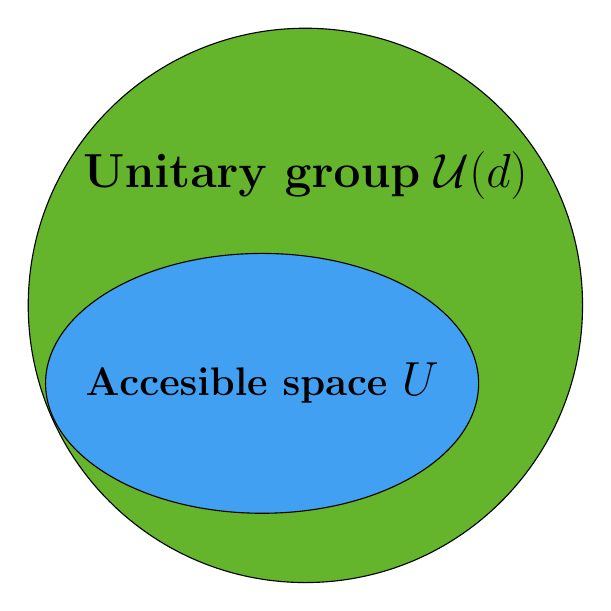
\begin{tikzpicture}[scale=1.1]
        \definecolor{circleColor}{RGB}{100,180,44}    % Green
        \definecolor{ellipseColor}{RGB}{65,160,241}   % Blue
        % Draw the circle
        \draw[fill=circleColor, draw=black] (0,0) circle (3.2cm);
        % Add text inside the circle
        \node at (0,1.5) {{\LARGE \textbf{Unitary group} $\calU(d)$}};
      
        % Draw the ellipse inside the circle
        \draw[fill=ellipseColor, draw=black] (-0.5,-0.9) ellipse (2.5cm and 1.5cm);
        % Add text inside the ellipse
        \node at (-0.5,-0.9) {{\LARGE \textbf{\Large Accesible space} $\bbU$}};
      \end{tikzpicture}
    \caption{ユニタリ群 $\calU(d)$ と量子回路の表現領域 $\bbU$}
    \label{fig:expressibility}
\end{figure}


\subsection{$p = 1$}
$p = 1$ のとき、$X$ として $\dyad{\bs{0}} := \dyad{0}\otn{n}$ を用いると、表現力は次のようになる。

\begin{align}
    \epsilon_{\bbU}^{(2,1)}(\dyad{\bs{0}}) &:= \norm{A^{(2)}(\dyad{\bs{0}})}_1\nonumber\\
    &= \Tr\abs{\int_{V\in\calU(d)} d\mu_{\Haar}(V)\,(V\dyad{\bs{0}}V\dg)\otn{2} - \int_{U\in\bbU} dU\,(U\dyad{\bs{0}}U\dg)\otn{2}}
\end{align}

トレースの第一項は以下のように計算される\cite{zhang2015matrix}。
\begin{align}
    \int_{V\in\calU(d)} d\mu_{\Haar}(V)\,(V\dyad{\bs{0}}V\dg)\otn{2} = \frac{\bbid_{d^2} + \SWAP}{d(d+1)},
\end{align}
ただし、$\SWAP := \sum_{i,j=1}^d \ket{ij}\bra{ji}$ である。


\subsection{$p = 2$}
$p = 2$ のとき、次の定理が成り立つ。
\begin{screen}
    \begin{theorem}
        表現力 $\epsilon_{\bbU}^{(t,2)}(X) = \norm{A^{(t)}(X)}_2$ は以下のようにフレームポテンシャルと呼ばれる量 $\calF$ によって表すことができる\cite{holmes2022connecting}。
        \begin{align}
            \epsilon_{\bbU}^{(t,2)}(X) &:= \sqrt{\calF_{\bbU}^{(t)}(X) - \calF_{\Haar}^{(t)}(X) }\\
            \calF_{\bbU}^{(t)}(X) &:= \int_{W\in\bbU}\int_{V\in\bbU} dWdV \Tr[WXW\dg (VXV\dg)\dg]^t\\
            \calF_{\Haar}^{(t)}(X)
            &:= \int_{W\in\calU(d)}\int_{V\in\calU(d)} d\mu_{\Haar}(W)d\mu_{\Haar}(V) \Tr[WXW\dg (VXV\dg)\dg]^t\nonumber\\
            &= \int_{V\in\calU(d)} d\mu_{\Haar}(V) \Tr[VX\dg V\dg X]^t
        \end{align}
        特に $t=2$ のとき、$\calF_{\calU(d)}^{(t)}(X)$ は、公式~\eqref{eq:haar-int-5} を用いて以下のように計算できる。
        \begin{align}
            \calF_{\Haar}^{(2)}(X) = \frac{\Tr[X^4] + \Tr[X^2]^2}{2^{2n} - 1} - \frac{2\Tr[X^2]\Tr[X]^2}{2^n(2^{2n} - 1)}
        \end{align}
    \end{theorem}
\end{screen}


\begin{proof}
    \begin{align}
        \qty{\epsilon_{\bbU}^{(t,2)}(X)}^2
        &:= \norm{A^{(t)}(X)}_2^2\\
        &:= \Tr\qty[A^{(t)}(X)\dg A^{(t)}(X)]\\
        &= \Tr\qty(\int_{V\in\calU(d)} d\mu_{\Haar}(V)\,(VX\dg V\dg)\otn{t} - \int_{U_1\in\bbU} dU_1\,(U_1X\dg U_1\dg)\otn{t}) \nonumber\\
        &\quad\; \times \qty(\int_{W\in\calU(d)} d\mu_{\Haar}(W)\,(WXW\dg)\otn{t} - \int_{U_2\in\bbU} dU_2\,(U_2XU_2\dg)\otn{t})\\
        &\overset{(1)}{=} \int_{V\in\calU(d)}\int_{W\in\calU(d)} d\mu_{\Haar}(V)d\mu_{\Haar}(W)\, \Tr[VX\dg V\dg WXW\dg]^t \nonumber\\
        &- \int_{V\in\calU(d)}\int_{U_2\in\bbU} d\mu_{\Haar}(V)dU_2\, \Tr[VX\dg V\dg U_2XU_2\dg]^t\nonumber\\
        &- \int_{U_1\in\bbU}\int_{W\in\calU(d)} dU_1d\mu_{\Haar}(W)\, \Tr[U_1X\dg U_1\dg WXW\dg]^t \nonumber\\
        &+ \int_{U_1\in\bbU}\int_{U_2\in\bbU} dU_1dU_2\, \Tr[U_1X\dg U_1\dg U_2XU_2\dg]^t\\
        &\overset{(2)}{=} \int_{V\in\calU(d)}\int_{W\in\calU(d)} d\mu_{\Haar}(V)d\mu_{\Haar}(W)\, \Tr[VX\dg V\dg X]^t \nonumber\\
        &- \int_{V\in\calU(d)}\int_{U_2\in\bbU} d\mu_{\Haar}(V)dU_2\, \Tr[VX\dg V\dg X]^t \nonumber\\
        &- \int_{U_1\in\bbU}\int_{W\in\calU(d)} dU_1d\mu_{\Haar}(W)\, \Tr[X\dg WXW\dg]^t \nonumber\\
        &+ \int_{U_1\in\bbU}\int_{U_2\in\bbU} dU_1dU_2\, \Tr[U_1X\dg U_1\dg U_2XU_2\dg]^t\\
        &\overset{(3)}{=} \int_{U_1\in\bbU}\int_{U_2\in\bbU} dU_1dU_2\, \Tr[U_1X\dg U_1\dg U_2XU_2\dg]^t \nonumber\\
        &- \int_{\calU(d)} d\mu_{\Haar}(V)\, \Tr[VX\dg V\dg X]^t\\
        &= \calF_{\bbU}^{(t)}(X) - \calF_{\Haar}^{(t)}(X)
    \end{align}
    等号(1)では、$A\otn{t} B\otn{t} = (AB)\otn{t}$ であることと、$\Tr[C\otn{t}] = \Tr[C]^t$ であることを用いた。等式(2)では、ハール分布の性質(両側不変性)を用いた。等式(3)では、$\int_{W\in\calU(d)} d\mu_{\Haar}(W) = \int_{U_{1,2}\in\bbU} dU_{1,2} = 1$ であることを用いた。
\end{proof}


\begin{screen}
    \begin{corollary}\label{cor:expressibility}
        $t = 2,\, X = \dyad{\bs{0}}$ のとき、表現力は次のように計算される\cite{holmes2022connecting}。
        \begin{align}\label{eq:expressibility-1}
            (\epsilon_{\bbU}^{(2,2)}(\dyad{\bs{0}}))^2 = \int_{W\in\bbU}\int_{V\in\bbU} dWdV |\bra{\bs{0}}W\dg V\ket{\bs{0}}|^4 - \frac{1}{2^{n-1}(2^n + 1)}
        \end{align}
    \end{corollary}
\end{screen}
式~\ref{eq:expressibility-1}の右辺の第一項をみると、これは対象となる量子回路から生成される2つの状態ベクトル $V\ket{\bs{0}},\,W\ket{\bs{0}}$ の内積の絶対値の4乗を積分(平均)したものであることがわかる。変分量子回路の表現力を数値計算で求める場合は、パラメーターをランダムにサンプリングして2つの状態ベクトルを生成し、それらの内積の絶対値の4乗を平均すればよい(モンテカルロ積分)。

\begin{proof}
    $X = \dyad{\bs{0}}$ のとき、$\calF_{\bbU}^{(2)}(\dyad{\bs{0}}),\, \calF_{\bbU}^{(2)}(\dyad{\bs{0}})$ は以下のように計算される。
    \begin{align}
        \calF_{\bbU}^{(2)}(\dyad{\bs{0}})
        &:= \int_{W\in\bbU}\int_{V\in\bbU} dWdV \Tr[W\dyad{\bs{0}}W\dg (V\dyad{\bs{0}}V\dg)\dg]^2\\
        &= \int_{W\in\bbU}\int_{V\in\bbU} dWdV |\bra{\bs{0}}W\dg V\ket{\bs{0}}|^4\\
        \calF_{\calU}^{(2)}(\dyad{\bs{0}})
        &:= \int_{W\in\calU}\int_{V\in\calU} d\mu_{\Haar}(W)d\mu_{\Haar}(V) \Tr[W\dyad{\bs{0}}W\dg (V\dyad{\bs{0}}V\dg)\dg]^2\\
        &= \int_{W\in\calU}\int_{V\in\calU} d\mu_{\Haar}(W)d\mu_{\Haar}(V) \Tr[(V\dg W)\dyad{\bs{0}} (V\dg W)\dg\dyad{\bs{0}}]^2\\
        &\overset{(1)}{=} \int_{W\in\calU}\int_{V\in\calU} d\mu_{\Haar}(W)d\mu_{\Haar}(V) \Tr[W\dyad{\bs{0}} W\dg\dyad{\bs{0}}]^2\\
        &\overset{(2)}{=} \int_{W\in\calU} d\mu_{\Haar}(W) \Tr[W\dyad{\bs{0}} W\dg\dyad{\bs{0}}]^2\\
        &= \int_{W\in\calU} d\mu_{\Haar}(W)\, \abs{\bra{\bs{0}}W\ket{\bs{0}}}^4\\
        &= \int_{W\in\calU} d\mu_{\Haar}(W)\, w_{\bs{0},\bs{0}}\,w_{\bs{0},\bs{0}}\,w^\ast_{\bs{0},\bs{0}}\,w^\ast_{\bs{0},\bs{0}}\\
        &\overset{(3)}{=} \frac{1}{2^{n-1}(2^n + 1)}
    \end{align}
    等号(1)では、ハール分布の性質(左不変性)を用いた。等号(2)では、$\int_{V\in\calU} d\mu_{\Haar}(V) = 1$ を用いた。等号(3)では、公式~\eqref{eq:haar-int-1} を用いた。
\end{proof}

% $p=2$ の場合、表現力は量子回路が生成するランダムな出力状態ベクトルの内積を積分することで計算できるが、$p=1$ の場合、表現力は密度演算子のテンソル積の積分が必要となる。したがって、$p=1$ の表現力は $p=2$ の表現力よりも計算コストが高い。


実際に系\ref{cor:expressibility}を用いて2つの具体的な量子回路に対して表現力 $(\epsilon_{\bbU}^{(2,2)}(\dyad{\bs{0}}))^2$ を計算してみる。
1つは、Tensor Product Ansatz (TPA) と呼ばれる回路であり、図~\ref{fig:tpa-alt}の左のような、2量子ビットゲートを持たない回路である。もう1つは、Alternating Layered Ansatz (ALT) と呼ばれる回路であり、図~\ref{fig:tpa-alt}の右のような、2量子ビットゲートを交互にずらして配置する量子回路である。

\begin{figure}[H]
    \centering
    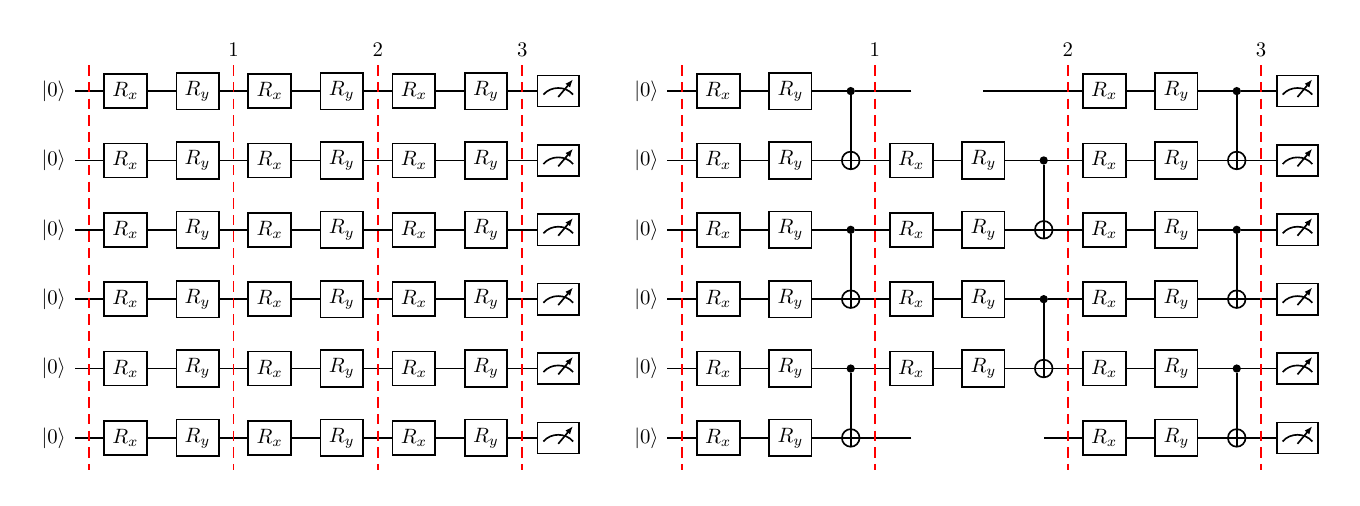
\begin{tikzpicture}
        \node[scale=0.75]{
        \begin{quantikz}
            \lstick{$\ket{0}$}\slice{} & \gate{R_x} & \gate{R_y}\slice{1}& \gate{R_x} & \gate{R_y}\slice{2}& \gate{R_x} & \gate{R_y}\slice{3}& \meter{}\\
            \lstick{$\ket{0}$}      & \gate{R_x} & \gate{R_y}      & \gate{R_x} & \gate{R_y}      & \gate{R_x} & \gate{R_y}      & \meter{}\\
            \lstick{$\ket{0}$}      & \gate{R_x} & \gate{R_y}      & \gate{R_x} & \gate{R_y}      & \gate{R_x} & \gate{R_y}      & \meter{}\\
            \lstick{$\ket{0}$}      & \gate{R_x} & \gate{R_y}      & \gate{R_x} & \gate{R_y}      & \gate{R_x} & \gate{R_y}      & \meter{}\\
            \lstick{$\ket{0}$}      & \gate{R_x} & \gate{R_y}      & \gate{R_x} & \gate{R_y}      & \gate{R_x} & \gate{R_y}      & \meter{}\\
            \lstick{$\ket{0}$}      & \gate{R_x} & \gate{R_y}      & \gate{R_x} & \gate{R_y}      & \gate{R_x} & \gate{R_y}      & \meter{}
        \end{quantikz}
        \qquad
        \begin{quantikz}
            \lstick{$\ket{0}$}\slice{}&\gate{R_x}&\gate{R_y}&\ctrl{1}\slice{1}&\qw       &          &\qw\slice{2}&\gate{R_x}&\gate{R_y}&\ctrl{1}\slice{3}& \meter{}\\
            \lstick{$\ket{0}$}        &\gate{R_x}&\gate{R_y}&\targ{}          &\gate{R_x}&\gate{R_y}&\ctrl{1}    &\gate{R_x}&\gate{R_y}&\targ{}          & \meter{}\\
            \lstick{$\ket{0}$}        &\gate{R_x}&\gate{R_y}&\ctrl{1}         &\gate{R_x}&\gate{R_y}&\targ{}     &\gate{R_x}&\gate{R_y}&\ctrl{1}         & \meter{}\\
            \lstick{$\ket{0}$}        &\gate{R_x}&\gate{R_y}&\targ{}          &\gate{R_x}&\gate{R_y}&\ctrl{1}    &\gate{R_x}&\gate{R_y}&\targ{}          & \meter{}\\
            \lstick{$\ket{0}$}        &\gate{R_x}&\gate{R_y}&\ctrl{1}         &\gate{R_x}&\gate{R_y}&\targ{}     &\gate{R_x}&\gate{R_y}&\ctrl{1}         & \meter{}\\
            \lstick{$\ket{0}$}        &\gate{R_x}&\gate{R_y}&\targ{}          &\qw       &          &            &\gate{R_x}&\gate{R_y}&\targ{}          & \meter{}
        \end{quantikz}
        };
    \end{tikzpicture}
    \caption{6量子ビット3層の TPA(左)と ALT(右)}
    \label{fig:tpa-alt}
\end{figure}

TPA の表現力の2乗した値を各量子ビット数 $n$、各層数 $L$ について計算した結果を図~\ref{fig:circuit-exp}の左に示す。ALT の表現力の2乗した値を各量子ビット数 $n$、各層数 $L$ について計算した結果を図~\ref{fig:circuit-exp}の右に示す。
表現力は、全てのパラメーターを $5000$ 回ランダムにサンプリングして計算した。

\begin{figure}[H]
    \begin{minipage}[b]{0.5\columnwidth}
        \centering
        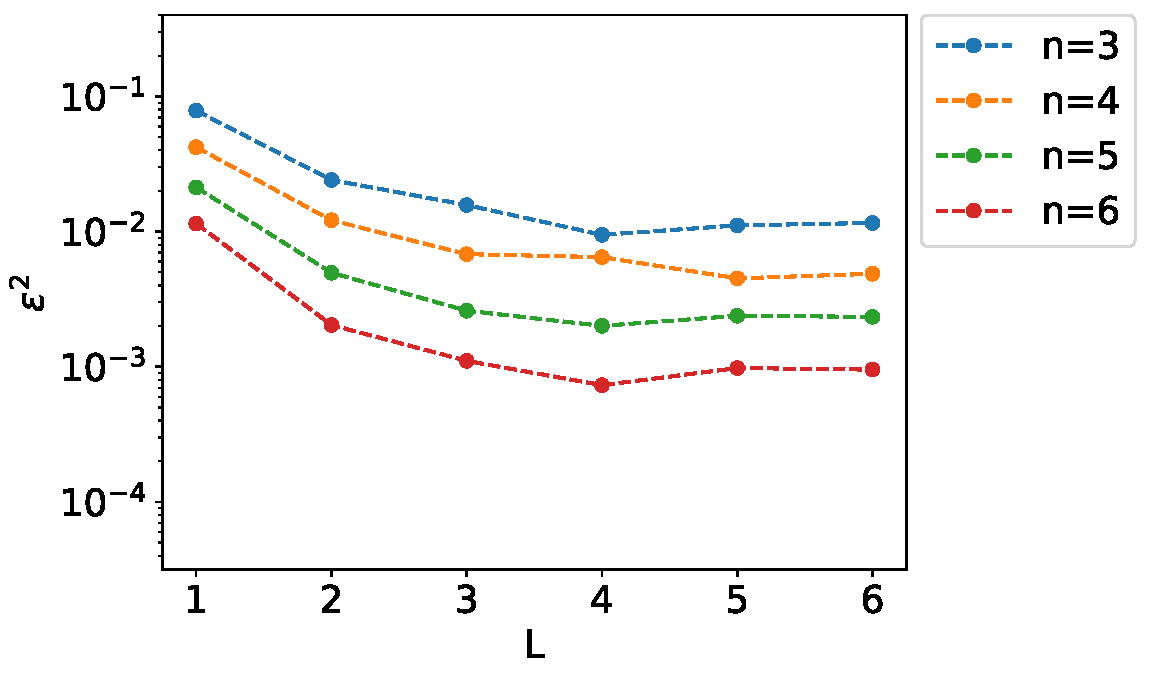
\includegraphics[width=8.5cm]{product-circuit-exp.pdf}
    \end{minipage}
    \hspace{0\columnwidth}
    \begin{minipage}[b]{0.5\columnwidth}
        \centering
        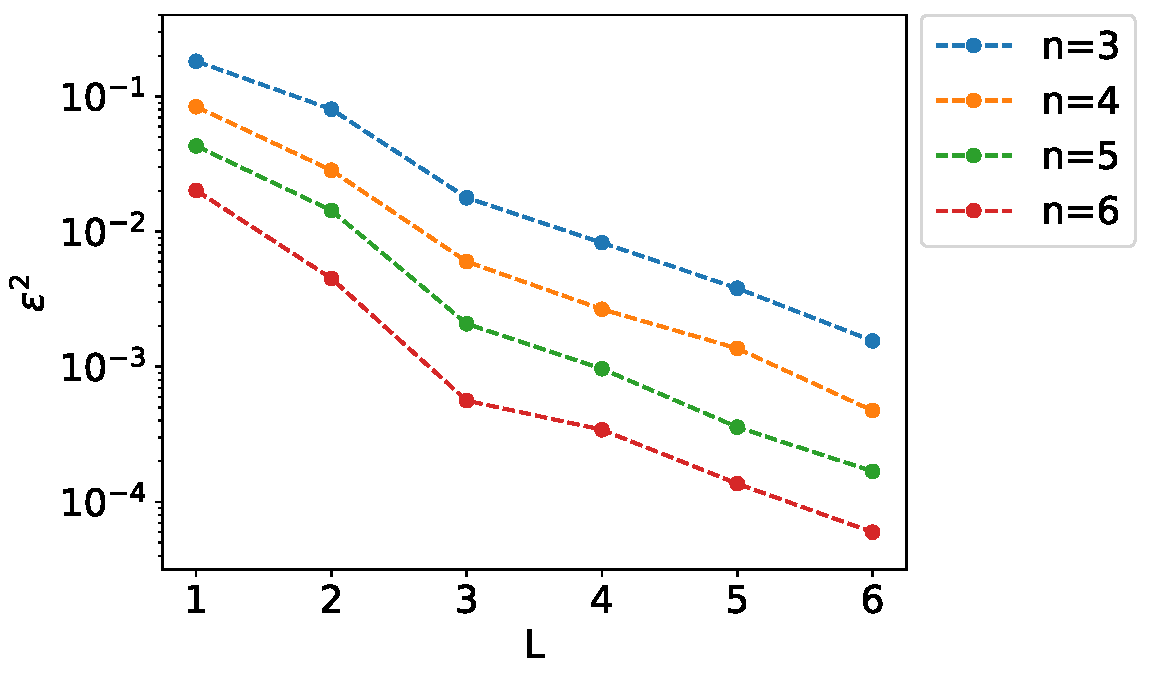
\includegraphics[width=8.5cm]{alt-circuit-exp.pdf}
    \end{minipage}
    \caption{TPA(左)と ALT(右)の表現力}
    \label{fig:circuit-exp}
\end{figure}

TPA はエンタングルメントを持たないため、一定以上の層数になると表現力がほとんど変化していない。一方、
ALT の総数を増やすほどエンタングルメントが増え、表現力が小さくなっていることがわかる。

\newpage
\chapter{量子機械学習におけるコスト関数の勾配の分散の上界}\label{chap:upper-bound}
量子機械学習におけるバレンプラトーの研究は、それ以外の変分量子アルゴリズムにおけるバレンプラトーの研究に比べて少ない\cite{thanasilp2021subtleties,thanasilp2022exponential}。特に、量子機械学習のデータの入力がバレンプラトーにどのように影響するかについては、詳しくわかっていない。そこで、この章では、量子機械学習におけるコスト関数の勾配の分散の上界をデータ入力の観点から調べた結果を示す。
まず、\ref{sec:qml-upper-var}~節では、勾配の分散の上界を、先行研究に基づき新たに導出する。\ref{sec:haar-random-input}~節では、入力状態がグローバルユニタリ $2$--デザインを成す場合の勾配の分散の上界を求める。\ref{sec:qml-var-expressibility}~節では、勾配の分散の上界を入力回路の表現力によって表す。\ref{sec:qml-var-local-2-design}~節では、入力状態がローカルユニタリ $2$--デザインを成すというグローバルユニタリ $2$--デザインよりも弱い仮定の下で、勾配の分散の上界を計算する。最後に、\ref{sec:qml-var-noise}~節では、\ref{sec:qml-var-local-2-design}~節の設定に加えて、Depolarizing ノイズがある場合の勾配の分散の上界を計算する。

本論文のバレンプラトーの解析においては、基本的に図~\ref{fig:qcl-setting}にあるような量子回路学習モデル(\ref{sec:quantum-circuit-learning}~節)を用いる。ただし、定理~\ref{thm:qml-upper-var}については Data reuploading モデル(\ref{sec:data-reuploading}~節)についても成り立つ。
量子カーネル法(\ref{sec:quantum-kernel}~節)に関するバレンプラトーについては、先行研究~\cite{thanasilp2022exponential}において既に解析されているため、本論文では扱わない。
\begin{figure}[H]
    \centering
    \begin{quantikz}
        \lstick{$\ket{0}$}     & \gate[wires=3][3cm]{{\LARGE U(\bs{x}_i)}} & \gate[wires=3][3cm]{{\LARGE V(\bs{\th})}} & \meter{}\\
        \lstick{$\vdots\;\;$}  & \wn &\wn & \wn\rstick{$\vdots$}\\
        \lstick{$\ket{0}$}     &     & \qw & \meter{}
    \end{quantikz}
    \caption{量子回路学習における量子回路の構造}
    \label{fig:qcl-setting}
\end{figure}

$\bs{x}_i$ はデータセット$\{(\bs{x}_i, y_i)\}_{i=1}^N$ の内、$i$ 番目の組の入力に対応するデータであり、$\bs{\th}$ は学習パラメーターである。$U(\bs{x}_i)$ はデータを入力するためのユニタリであり、$V(\bs{\th})$ は学習パラメーターを入力するためのユニタリである。ただし、全てのパラメーター $\bs{\th} = (\th_1,\th_2,
\cdots)$ は独立であり、取りうる区間は $[0, 2\pi]$ であると仮定する。

データ入力後の量子状態の密度演算子を $\rho_i = U(\bs{x}_i)\dyad{\bs{0}}U\dg(\bs{x}_i)$ と表し、これを入力状態と呼ぶ。また、学習パラメーター入力後の量子状態の密度演算子を $\rho_i(\bs{\th}) = V(\bs{\th})U(\bs{x}_i)\dyad{\bs{0}}U\dg(\bs{x}_i)V\dg(\bs{\th})$ とする。

以降の解析においては、$\bbU := \{U(\bs{x})|\,\bs{x}\in \calX \subset \bbR^m,\, m \in \bbN\}$ とする。すなわち、$\bbU$ は入力データ $\bs{x}$ によって生成されるユニタリの集合である。
関数 $g(U(\bs{x}))$ の入力データ $\bs{x}\in \calX$ に関する積分は、次のように $U\in\bbU$ に関する積分として表現する。
\begin{align}
    \int_{\bbU} dU\,g(U) = \int_{\calX} d\bs{x}\,g(U(\bs{x}))
\end{align}


\section{量子機械学習における勾配の分散の一般的な上界}\label{sec:qml-upper-var}
バレンプラトーに関連するほとんどの論文では、コスト関数は式~\eqref{eq:cost-simple} のように、あるオブザーバブルの期待値として与えられる(VQEやQAOAなどの典型的な変分量子アルゴリズムにおけるコスト関数)。一方、教師ありの量子機械学習においては式~\eqref{eq:cost-ml} のように、各訓練データに依存する出力 $\ell_i(\bs{\th})$ それ自体、あるいは更に関数を作用させたものをモデルの予測としてコスト関数が定義される。このようなコスト関数に関するバレンプラトーの先行研究はまだ少ない。
\begin{align}
    \ell_i(\bs{\th}) &= \Tr[\rho_i(\bs{\th})\,O], \label{eq:cost-simple}\\
    \calL(\bs{\th}) &= \frac1N\sum_{i=1}^N f(\ell_i(\bs{\th}),y_i) \label{eq:cost-ml}
\end{align}
ただし、$f$ は $f(x,y) := \abs{x - y}$ や $f(x,y) := (x-y)^2$、$f(x,y) := -y\log{x} - (1-y)\log{(1-x)}$ などの関数であり、
$O$ は任意のオブザーバブルである。
% \memo{この時点で、$\ell_x(\bs{\th}) = \Tr[\rho_x(\bs{\th})\,O]$,$\calL = \E_\calX[f(\ell_i(\bs{\th}),y_i)]$と定義しておけばいいかも\cite{barthe2023gradients}}

$\ell_i(\bs{\th})$ の勾配は、パラメーターシフトルール(\ref{sec:parameter-shift-rule}~節)によって求めることができる。一方、$\calL(\bs{\th})$ の勾配は、$\pd_\nu := \pd/\pd\th_\nu$  として、次のように連鎖律によって求める。
\begin{align}\label{eq:qml-chain-rule}
    \pd_\nu \calL(\bs{\th}) =  \sum_{i=1}^N \pd_{\ell_i(\bs{\th})} f \cdot \pd_\nu \ell_i(\bs{\th}).
\end{align}

この勾配の計算量が量子ビット数に関してどのようにスケールするかを調べることは、量子機械学習の計算量の評価において重要である。よって、バレンプラトーの定義にもあるように、この勾配の分散 $\Var_{V(\bs{\th})}\qty[\pd_\nu \calL(\bs{\th})]$ を調べる。まず、分散の公式を用いて式~\eqref{eq:qml-chain-rule}を次のように変形してみる。
\begin{align}
    \Var_{V(\bs{\th})}\qty[\pd_\nu \calL(\bs{\th})]
    &= \Var_{V(\bs{\th})}\qty[\frac1N\sum_{i=1}^N \pd_\nu f(\ell_i(\bs{\th}),y_i)]\nonumber\\
    &= \frac{1}{N^2} \sum_{i,j=1}^N \Cov_{V(\bs{\th})}[\pd_\nu f(\ell_i(\bs{\th}),y_i), \pd_\nu f(\ell_j(\bs{\th}),y_j)]
\end{align}
すると、$\Var_{V(\bs{\th})}\qty[\pd_\nu \calL(\bs{\th})]$ は $\pd_\nu f(\ell_i(\bs{\th}),y_i)$ の共分散に分解できる。共分散は負の値を取りうるため、$\Var_{V(\bs{\th})}\qty[\pd_\nu \calL(\bs{\th})]$ のスケーリングが $\Var_{V(\bs{\th})}\qty[\pd_\nu \ell_i(\bs{\th})]$ のスケーリングと同じとは限らないことがわかる。

$\Var_{V(\bs{\th})}\qty[\pd_\nu \calL(\bs{\th})]$ の性質に関して、先行研究~\cite{thanasilp2021subtleties}により次の結果が得られている。

\begin{screen}
    \begin{theorem}\label{thm:qml-upper-var-sutlties}
        (論文~\cite{thanasilp2021subtleties}の Theorem 1 の結果)
        量子機械学習におけるコスト関数 $\calL(\bs{\th}) = \sum_{i=1}^N f(\ell_i(\bs{\th};y_i),y_i)$ のパラメーター $\th_\nu \in \bs{\th}$ に関する勾配 $\pd_\nu \calL(\bs{\th}) \equiv \pd \calL(\bs{\th})/\pd \th_\nu$ の分散は次のように上から抑えられる。
        \begin{align}\label{eq:qml-upper-var-sutlties}
            \Var_{V(\bs{\th})}[\pd_\nu\calL(\bs{\th})] \leq \qty(\frac1N \sum_{i=1}^N g_i \sqrt{\Var_{V(\bs{\th})}[\pd_\nu \ell_i(\bs{\th})] + (\E_{V(\bs{\th})}[\pd_\nu \ell_i(\bs{\th})])^2 })^2
        \end{align}
        
        ここで、$\ell_i(\bs{\th}) \equiv \ell_i(\bs{\th};y_i)$ であり、平均と分散はパラメーター $\bs{\th}$ に関して取られている。また、$g_i$ は以下のように定義される。
        \begin{align}
            g_i = \sqrt{2} \max_{\ell_i} \abs{\pdv{f}{\ell_i}}
        \end{align}
        
        ここで、$\max_{\ell_i} \abs{\pd f/\pd \ell_i}$ は $f(\ell_i, y_i)$ の偏微分の絶対値の最大値である。
    \end{theorem}
\end{screen}

この定理は、$\ell_i(\bs{\th})$ の勾配の分散の解析を $\calL(\bs{\th})$ の勾配の分散の解析に適用できることを示した最初の結果であった。例えば、全ての $i$ について $\ell_{i}(\bs{\th})$ がバレンプラトーになるとすると、
\begin{align}
    \E_{V(\bs{\th})}[\pd_\nu\ell_i(\bs{\th})] = 0, \quad
    \Var_{V(\bs{\th})}[\pd_\nu\ell_i(\bs{\th})] \in \order{2^{-\alpha\,n}},\quad 0<\alpha \quad \text{for all $i$}
\end{align}
が成り立つ。よって、全ての $i$ について $g_{i} \in \order{\poly(n)}$ であるならば、上界~\eqref{eq:qml-upper-var-sutlties}は $\order{2^{-\alpha\,n}}$ となる。したがって、$\calL(\bs{\th})$ もバレンプラトーとなる。

本研究では、上界について次の定理\ref{thm:qml-upper-var}を導いた。
上界\eqref{eq:qml-upper-var-1}は上界\eqref{eq:qml-upper-var-sutlties}よりも緩いが、具体的な回路に対して上界を解析的に計算することができる。
\begin{screen}
    \begin{theorem}\label{thm:qml-upper-var}
        Theorem \ref{thm:qml-upper-var-sutlties}と同じ仮定の下、次の不等式が成り立つ。
        \begin{align}\label{eq:qml-upper-var-1}
            \Var_{V(\bs{\th})}[\pd_\nu \calL(\bs{\th})]
            &\leq
            2\max_{i,\bs{\th}} [(\pd_{\ell_i(\bs{\th})}f)^2]
            \times
            % \frac1N\sum_i \Var[\pd_\nu \ell_i(\bs{\th})]
            \int_{U\in\bbU} dU \Var_{V(\bs{\th})}[\pd_\nu \ell(\bs{\th})]
        \end{align}
    \end{theorem}
\end{screen}

この定理の証明においては、次の補題を用いる。証明は論文\cite{thanasilp2022exponential}の Lemma 1, 5 を参照されたい。
\begin{screen}
    \begin{lemma}\label{lem:variance-inequality}
        分散についての以下の不等式が成り立つ。
        \begin{align}
            \Var\Big[\sum_i X_i\Big] &\leq N\sum_i\Var[X_i],\label{eq:sum-variance}\\
            \Var[XY] &\leq 2\Var[X]\abs{Y^2}_{\max} + 2(\E[X])^2\Var[Y]\,.\label{eq:prod-variance}
        \end{align}
    \end{lemma}
\end{screen}

\begin{proof}\label{proof:qml-upper-var}
    まず、$\E_{V(\bs{\th})}\qty[\pd_\nu \ell_i(\bs{\th})] = 0$ を示す。ここでは、定理\ref{thm:bp}と同じように、$\ell_i(\bs{\th}) := C(\bs{\th}) = \Tr[\rho_i(\bs{\th})O]$, $V(\bs{\th}) = V_+V_-$, $V_+ := \prod_{l=k+1}^L U_l(\th_l)W_l$, $V_- := \prod_{l=1}^{k} U_l(\th_l)W_l$ とする。また、証明~\ref{proof:bp}で得られるように、次の等式が成り立つ。
    \begin{align}
        \pd_\nu \ell_i(\bs{\th})
        &=\frac{i}{2}\Tr[V_-\rho V_-\dg\, [P_k, V_+\dg OV_+]]
    \end{align}
    
    簡単のため、 $c = \cos(\th_\nu/2),\, s = \sin(\th_\nu/2)$ とする。このとき、$\pd_\nu \ell_i(\bs{\th})$ は次のように展開できる。
    \begin{align}
        \pd_\nu \ell_i(\bs{\th})
        &= \frac{i}{2}\Tr[V_-\rho V_-\dg\, [P_k, V_+\dg OV_+]]\\
        &= \frac{i}{2}\Tr[\qty(c\,\bbid - i\,sP_k)W_k\qty(\prod_{l=1}^{k-1}U_lW_l)\rho \qty(\prod_{l=1}^{k-1}U_lW_l)\dg W_k\dg\qty(c\,\bbid - i\,sP_k)\dg\, [P_k, V_+\dg OV_+]]\\
        &= \frac{i}{2}\qty{(c^2-s^2)\Tr[[\rho^\prime, P_k]V_+\dg OV_+] + i\,cs\Tr[[\rho^\prime, P_k]]}
    \end{align}
    ただし、$\rho^\prime = W_k\qty(\prod_{l=1}^{k-1}U_lW_l)\rho \qty(\prod_{l=1}^{k-1}U_lW_l)\dg W_k\dg$ とした。
    $\th_\nu \in [0,2\pi]$ による平均は、
    \begin{align}
        \frac{1}{2\pi}\int_0^{2\pi} d\th_\nu\, (c^2-s^2) = 0, \quad
        \frac{1}{2\pi}\int_0^{2\pi} d\th_\nu\, cs = 0
    \end{align}
    である。よって、$\E_{V(\bs{\th})}\qty[\pd_\nu \ell_i(\bs{\th})] = 0$ である。
    
    次に $\Var_{V(\bs{\th})}[\pd_\nu \calL(\bs{\th})]$ の上界を導く。
    \begin{align}
        \Var_{V(\bs{\th})}\qty[\pd_\nu \calL(\bs{\th})]
        &= \Var_{V(\bs{\th})}\qty[\frac1N\sum_{i=1}^N \pd_\nu f(\ell_i(\bs{\th}),y_i)]\\
        &\overset{(1)}{\leq} \frac1N\sum_{i=1}^N \Var_{V(\bs{\th})}[\pd_\nu f(\ell_i(\bs{\th}),y_i)]\\
        &= \frac1N\sum_{i=1}^N \Var_{V(\bs{\th})}[\pd_{\ell_i(\bs{\th})}f \cdot \pd_\nu \ell_i(\bs{\th})]\\
        &\overset{(2)}{\leq} \frac1N\sum_{i=1}^N 2\max_{\bs{\th}}[(\pd_{\ell_i(\bs{\th})}f)^2] \cdot \Var_{V(\bs{\th})}[\pd_\nu \ell_i(\bs{\th})]\\
        &\leq 2\max_{i,\,\bs{\th}}[(\pd_{\ell_i(\bs{\th})}f)^2] \times \frac1N\sum_{i=1}^N \Var_{V(\bs{\th})}[\pd_\nu \ell_i(\bs{\th})]\\
        &=: 2\max_{i,\bs{\th}} [(\pd_{\ell_i(\bs{\th})}f)^2]
        \times \int_{U\in\bbU} dU \Var_{V(\bs{\th})}[\pd_\nu \ell(\bs{\th})]
    \end{align}
    
    ただし、不等式(1)では、不等式\eqref{eq:sum-variance}を用いた。不等式(2)では、不等式\eqref{eq:prod-variance}と $\E_{V(\bs{\th})}\qty[\pd_\nu \ell_i(\bs{\th})] = 0$ を用いた。
\end{proof}


この結果から、コスト関数の勾配の分散の上界を求めるためには、$\int_{U\in\bbU} dU \Var_{V(\bs{\th})}[\pd_\nu \ell(\bs{\th})]$ を計算する必要があるとわかる。具体的なスケーリングを求めるため、以降の解析においては、図~\ref{fig:circuit-setting}の構造を仮定する。すなわち、初めは入力回路には条件を課さず、学習回路のみ $\xi$ 個の $s$ 量子ビットユニタリのテンソル積からなる回路であるとする。
\begin{figure}[H]
    \centering
    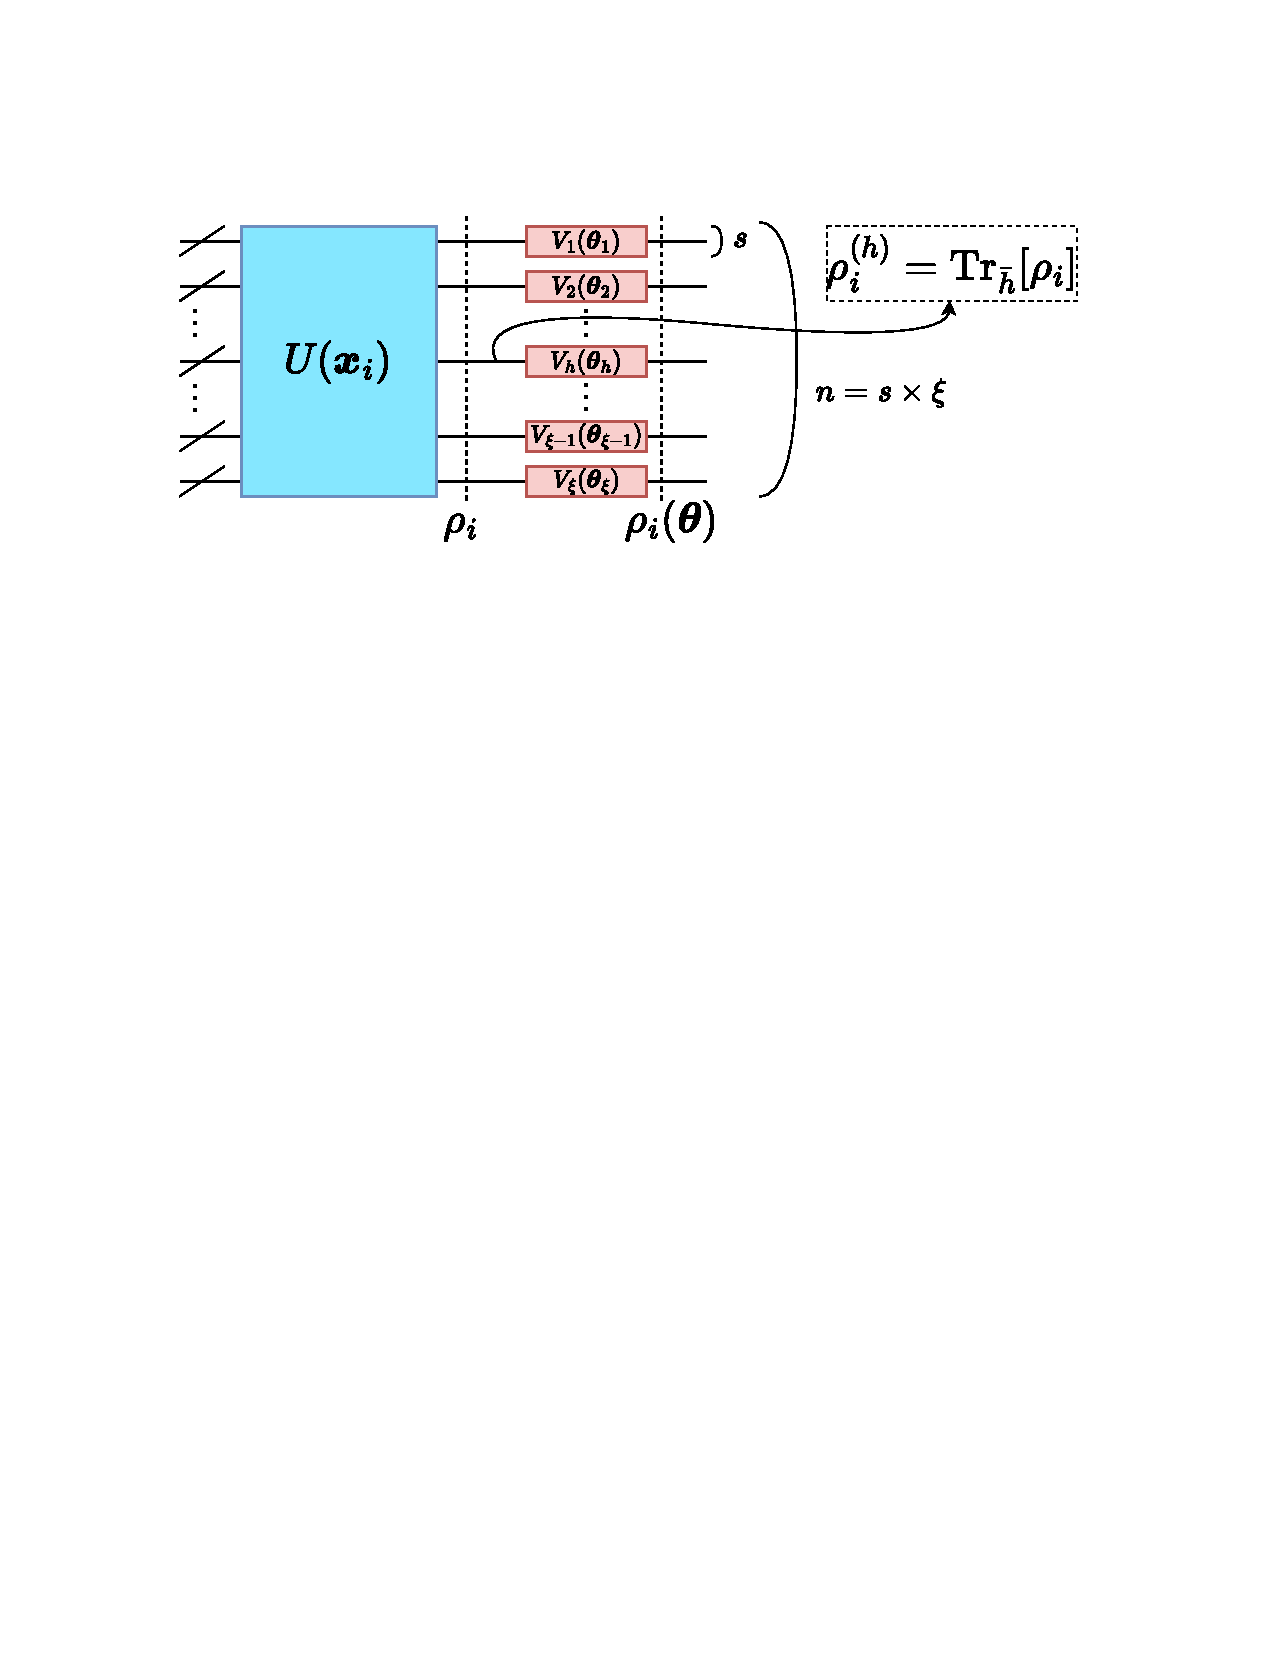
\includegraphics[width=16cm]{setting.pdf}
    \caption{解析する量子回路の構造:学習回路は $s$ 量子ビットユニタリのテンソル積からなる}
    \label{fig:circuit-setting}
\end{figure}

この学習回路の各 $s$ 量子ビットユニタリがそれぞれユニタリ $2$--デザインを成す、すなわち、ローカルユニタリ $2$--デザインを成すと仮定する。
このとき、次の命題が成り立つことが先行研究~\cite{cerezo2021cost}により示されている。
\begin{screen}
    \begin{proposition}\label{prop:qml-var-local-2-design}
        (論文~\cite{cerezo2021cost}の Supplementary Note 5, B の結果) 
        $V(\bs{\th})$ が、$s$ 量子ビットユニタリのテンソル積からなり、それぞれがローカルユニタリ $2$--デザインを成すと仮定する。コスト関数 $\ell_i(\bs{\th}) = \Tr[\rho_i(\bs{\th})O_\rmL],\,O_\rmL = \frac{1}{n} \sum_{j=1}^{n}\dyad{0}_{j} \otimes \bbid_{\bar{j}}$ について、$h$ 番目のゲートブロック中のパラメーター $\th_\nu$ 関する偏微分を考える。このとき、次の等式が成り立つ。
        \begin{align}
            \Var_{V(\bs{\th})}[\pd_\nu \ell_i(\bs{\th})] = r_{n,s}D_{\HS}(\rho_i^{(h)} , \bbid/2^s )\label{eq:ell-var}
        \end{align}
        ここで、$r_{n,s} := \frac{s\cdot 2^{3(s-1)}}{n^2(2^{2s}-1)^2} \in \Omega(1/\poly(n))$ であり、$D_{\HS}(A, B) = \Tr[(A - B)^2]$ は Hilbert--Schmidt 距離である。また、$\bbid/2^s$ は $s$ 量子ビット上の最大混合状態であり、$\rho_i^{(h)} = \Tr_{\bar h}[U(\bs{x}_i)\dyad{\bs{0}}U\dg(\bs{x}_i)]$ は $h$ 番目のユニタリが作用する $s$ 量子ビット上の入力状態の縮約密度演算子である。
    \end{proposition}
\end{screen}

この命題において、学習回路とオブザーバブルの情報は $r_{n,s}$ に含まれるが、$s$ は $n$ によらず、オブザーバブルは局所的なものであるため、これらはバレンプラトーの原因とならない。
一方で、この命題は、入力状態の縮約密度演算子 $\rho_i^{(h)}$ が最大混合状態に近いほど、$\Var_{V(\bs{\th})}[\pd_\nu \ell_i(\bs{\th})]$ が小さくなることを意味する。つまり、式~\eqref{eq:ell-var}は、データセットと入力回路の構造の情報を含む $\rho_i$ がバレンプラトーを引き起こす可能性があることを意味する。

式~\eqref{eq:ell-var}を式~\eqref{eq:qml-upper-var-1}に代入すると、次の上界を得る。
\begin{align}\label{eq:qml-upper-var-2}
    \Var_{V(\bs{\th})}[\pd_\nu \calL(\bs{\th})]
    &\leq
    2\max_{i,\bs{\th}} [(\pd_{\ell_i(\bs{\th})}f)^2]
    \times r_{n,s} \times
    \int_{U\in\bbU} dU D_{\HS} (\rho^{(h)} , \bbid/2^s ).
\end{align}

よって、$\int_{U\in\bbU} dU D_{\HS} (\rho^{(h)} , \bbid/2^s)$ が上界のスケーリングを決めることがわかる。

\begin{comment}
    \section{Connect two papers results}
    \cite{cerezo2021cost,thanasilp2021subtleties}When QNN is giben by a single layer of the alternating layered ansatz made of a tensor product of s-qubit unitaries and a local cost function is
    $$
        \ell_i(\bs{\th}) = 1 - \frac{1}{n}\sum_{j=1}^n \Tr[(\dyad{0}_j \ot \bbid_{\bar{j}} ) \rho_i(\bs{\th})] ,
    $$
    the $\Var_{V(\bs{\th})}[\pd_\nu\, \ell_i(\bs{\th})]$ is given by

    \begin{align}
        \Var_{V(\bs{\th})}[\pd_\nu\, \ell_i(\bs{\th})] = r_{n,s}\,D_{\HS}(\rho_i^{(h)},\, \bbid/2^s),\quad r_{n,s} = \frac{s\cdot 2^{3(s-1)}}{n^2(2^{2s}-1)^2} \in \Omega\qty(\frac{1}{\poly(n)}).
    \end{align}

    Using the inequality in \textbf{Theorem 2}, $\Var_{V(\bs{\th})}[\pd_\nu\, \ell_i(\bs{\th})]$ is bounded as follows.
    \begin{align}
        \frac{r_{n,s}}{d}\,D_2(\rho_i^{(h)},\, \bbid/2^s) \leq \Var_{V(\bs{\th})}[\pd_\nu\, \ell_i(\bs{\th})] \leq \frac{r_{n,s}}{e}\,D_2(\rho_i^{(h)},\, \bbid/2^s).
    \end{align}

    In a kind of circuits, $D_2(\rho,\, \bbid/2^s)$ is shown to be exponentially small with respect to the number of embedding layers~\cite{thanasilp2022exponential}.
    We have to note that the some assumptions are different in these two papers~\cite{thanasilp2022exponential,cerezo2021cost}. However, If we were able to show that $\bbV[\pd_\nu\, \ell_i(\bs{\th})]$ is given by the form of $r_{n,s}\,D_{\HS}(\rho_i,\, \bbid/2^s)$ and $D_2(\rho_i,\, \bbid/2^s) \in \Omega\qty(e^{-\alpha n})\, (\alpha>0)$ for the same conditions, it shows the effect of encoding on barren plateaus.
\end{comment}



\section{グローバルユニタリ $2$--デザインの入力状態とバレンプラトー}\label{sec:haar-random-input}
バレンプラトーの解析においては、しばしば、学習回路がグローバルユニタリ $2$--デザインを成すと仮定する。そこで、$\int_{U\in\bbU} dU D_{\HS} (\rho^{(h)} , \bbid/2^s)$ を計算する最初の簡単なモデルとして、入力状態の集合がグローバルユニタリ $2$--デザインを成すと仮定する。
$D_{\HS} (\rho , \bbid/2^s) = \Tr[\rho^2] - 1/2^s$ であることから、
\begin{align}
    D_{\HS}(\rho^{(h)},\bbid/2^s) = \Tr[(\Tr_{\bar{h}}[U\dyad{\bs{0}} U\dg])^2] - 1/2^s
\end{align}
であり、最初の項は $U,\,U\dg$ の成分に関してそれぞれ2次の多項式である。よって、ユニタリ $2$--デザインの定義から次のように $\bbU = \calU(d),\, dU = d\mu_{\Haar}(U)$ として積分してよい。
\begin{align}
    \int_{U\in\calU(d)} d\mu_{\Haar}(U) D_{\HS}(\rho^{(h)},\bbid/2^s)
    = \int_{U\in\calU(d)} d\mu_{\Haar}(U) \Tr[(\Tr_{\bar{h}}[U\dyad{\bs{0}} U\dg])^2] - 1/2^s 
\end{align}
となる。右辺の第一項の積分計算は、次の定理により与えられる。

\begin{screen}
    \begin{theorem}\label{thm:dhs-haar-int}
        $\calH$ を $\calH = \calH_h \ot \calH_{\overline{h}}$ のように二つの系からなる $n$ 量子ビットの Hilbert 空間とする。ここで、$\calH_h$ は $s$ 量子ビットからなる Hilbert 空間であり、$\calH_{\overline{h}}$ は残りの $n-s$ 量子ビットからなる Hilbert 空間である。このとき、次の式が成り立つ。
        \begin{align}
            \int_{U\in\calU(d)}\Tr_h[(\Tr_{\bar{h}}[U\dyad{\bs{0}}U\dg])^2] dU
            =
            \frac{2^{n-s} + 2^{s}}{2^n+1}.
        \end{align}
    \end{theorem}
\end{screen}

\begin{proof}
    $ a_{ij} = U_{i1}U_{j1}^*,\,\,t = 2^{n-s}$ とすると、
    \begin{align}
        &\Tr_{\bar{h}}[U\dyad{\bs{0}}U\dg]=\nonumber\\
        &\begin{bmatrix}
            a_{1,1}+a_{2,2}+\cdots+a_{t,t} & a_{1,t+1}+a_{2,t+2}+\cdots+a_{t,2t}& \cdots & a_{1,2^n-t+1}+a_{2,2^n-t+2}+\cdots+a_{t,2^n}\\
            a_{t+1,1}+a_{t+2,2}+\cdots+a_{2t,t} & a_{t+1,t+1}+a_{t+2,t+2}+\cdots+a_{2t,2t} & \cdots & a_{t+1,2^n-t+1}+a_{t+2,2^n-t+2}+\cdots+a_{2t,2^n}\\
            \cdots & \cdots & \cdots & \cdots\\
            a_{2^n-t+1,1}+\cdots+a_{2^n,t} & a_{2^n-t+1,t+1}+\cdots+a_{2^n,2t} & \cdots & a_{2^n-t+1,2^n-t+1}+\cdots+a_{2^n,2^n}.
        \end{bmatrix}
    \end{align}
    よって、上の行列の二乗 $(\Tr_{\bar{h}}[U\dyad{\bs{0}}U\dg])^2$ の(1,1)成分は以下のようになる。
    \begin{align}
        (a_{1,1}+a_{2,2}+\cdots+a_{t,t})^2 + (a_{1,t+1}+a_{2,t+2}+\cdots+a_{t,2t})(a_{t+1,1}+a_{t+2,2}+\cdots+a_{2t,t})\nonumber\\
        \cdots + (a_{1,2^n-t+1}+\cdots+a_{t,2^n})(a_{2^n-t+1,1}+\cdots+a_{2^n,t})
    \end{align}
    
    ユニタリ $2$--デザインの定義から、ハール分布の積分公式~\eqref{eq:haar-int-2}を用いることができ、
    \begin{align}
        \int_{U\in\calU(d)}d\mu_{\Haar}(U)\,a_{ij}a_{i^\prime j^\prime} = \frac{1}{d(d+1)}(\delta_{ij}\delta_{i^\prime j^\prime} + \delta_{ij^\prime}\delta_{i^\prime j})
    \end{align}
    が成り立つ。よって、$a_{p,p}a_{p,p},\,a_{p,p}a_{q,q},\,a_{p,q}a_{q,p}\,(p \neq q)$ のみが生き残る。他の対角成分も同様であるから、求める式は以下のようになる。
    
    \begin{align}
        &\int_{U\in\calU(d)}\Tr[(\Tr_{\bar{h}}[U\dyad{\bs{0}}U\dg])^2] d\mu_{\Haar}(U)\nonumber\\
        &=\int_{U\in\calU(d)}d\mu_{\Haar}(U)
        \qty(
            \qty[\sum_{i=1}^t a_{ii}^2]
            + \qty[2\sum_{i<j}^t a_{ii}a_{jj}]
            + \underbrace{\qty[\sum_{i=1}^t a_{t+i,i}a_{i,t+i}] + \cdots + \qty[\sum_{i=1}^t a_{2^n-t+i,i}a_{i,2^n-t+i}]}_{2^s-1 \text{ 個}}
        ) \times 2^s\\
        &=\int_{U\in\calU(d)}d\mu_{\Haar}(U) \qty(\qty[\sum_{i=1}^t a_{ii}^2] + \qty[2\sum_{i<j}^t a_{ii}a_{jj}] + \qty[\sum_{i=1}^t a_{t+i,i}a_{i,t+i}] \times (2^s - 1)) \times 2^s\\
        &=\qty(t\times \frac{2}{d(d+1)} + 2\times \combi{t}{2}\times\frac{1}{d(d+1)} + t\times \frac{1}{d(d+1)} \times (2^s - 1)) \times 2^s\\
        &=\frac{2^{n-s} + 2^s}{2^n + 1}
    \end{align}
    
    % \footnote{他の証明方法については、公式~\eqref{fig:haar-int-4}、論文~\cite{low2009large} の Lemma 4.1、論文~\cite{zhang2014matrix} の Remark 3.12、論文~\cite{zhang2022fundamental} の Corollary S3 を参照。}
\end{proof}


この定理より、
\begin{align}
    \int_{U\in\calU(d)} d\mu_{\Haar}(U) D_{\HS}(\rho^{(h)},\bbid/2^s)
    &= \int_{U\in\calU(d)} d\mu_{\Haar}(U) \Tr[(\Tr_{\bar{h}}[U\dyad{\bs{0}} U\dg])^2] - 1/2^s \nonumber\\
    &= \frac{2^{n-s} + 2^s}{2^n + 1} - 1/2^s \nonumber\\
    &= \frac{2^s - 2^{-s}}{2^n + 1} \,\in [0,1 - 1/2^s]\\
    &=: \calD_{\Haar}
\end{align}

したがって、入力状態の集合がグローバルユニタリ $2$--デザインを成す場合の上界は次で与えられる。
\begin{align}\label{eq:qml-upper-var-haar}
    \Var_{V(\bs{\th})}[\pd_\nu \calL(\bs{\th})]
    &\leq
    2\max_{i,\bs{\th}} [(\pd_{\ell_i(\bs{\th})}f)^2]
    \times r_{n,s}
    \times \frac{2^s - 2^{-s}}{2^n + 1} \,\in \order{\frac{1}{2^n}}
\end{align}
以上より、量子回路の構造は図~\ref{fig:circuit-setting}で与えられ、学習回路やオブザーバブルがパレンプラトーを引き起こさないとしても、入力状態の集合がグローバルユニタリ $2$--デザインを成す場合は、コスト関数はバレンプラトーとなることが分かった。



\section{入力回路の表現力による上界}\label{sec:qml-var-expressibility}
この節では、上界\eqref{eq:qml-upper-var-2} のうち $\int_{U\in\bbU} dU D_{\HS} (\rho^{(h)} , \bbid/2^s )$ の項が、前節で得た結果 
$$
    \calD_{\Haar} = \frac{2^s - 2^{-s}}{2^n + 1}
$$
と入力回路の表現力によって、次のように上から抑えられることを示す。
$$
    \int_{U\in\bbU} dU D_{\HS} ( \rho^{(h)} ,\, \bbid/2^s ) \leq \calD_{\Haar} + \epsilon_{\bbU}^{(2,1)}(\dyad{0})
$$
この不等式により、入力回路の表現能力が高いほど、上界がきつくなることが定性的に理解される。

まず、その証明に必要な2つの補題を示す。
\begin{screen}
    \begin{lemma}\label{lemma:swap1}
        密度演算子 $\rho_A \in \calS(\calH_A)  ,\,\rho_B \in \calS(\calH_B) \; (\dim{\calH_A} = \dim{\calH_B})$ に対して、次の等式が成り立つ。
        \begin{align}\label{eq:swap1}
            \Tr_A[\SWAP\,(\rho_A \ot \rho_B)] = \rho_A\,\rho_B
        \end{align}
        ただし、$\SWAP := \sum_{i,j=1}^d \kten{i}{j}\bten{j}{i}, \eg \SWAP\,\kten{x_i}{y_j} = \kten{y_j}{x_i}$ である。
    \end{lemma}
\end{screen}

\begin{proof}
    $\rho_A$ と $\rho_B$ は、それぞれ $\rho_A = \sum_{i=1}^d \lambda_i \dyad{x_i}$ と $\rho_B = \sum_{i=1}^d \mu_i \dyad{y_i}$ のように固有分解されると仮定する。これを $\Tr_A[\SWAP\,(\rho_A \ot \rho_B)]$ に代入すると、
    \begin{align*}
        \Tr_A[\SWAP\,(\rho_A \ot \rho_B)]
        &= \Tr_A\qty[\SWAP\,\qty(\sum_{i,j=1}^d \lambda_i \mu_j (\kten{x_i}{y_j})(\bten{x_i}{y_j}))]\\
        &= \Tr_A\qty[\sum_{i,j=1}^d \lambda_i \mu_j (\kten{y_j}{x_i})(\bten{x_i}{y_j})]\\
        &= \sum_{i,j=1}^d \lambda_i \mu_j \Tr_A[\dyad{y_j}{x_i}]\,\dyad{x_i}{y_j}\\
        &= \sum_{i,j=1}^d \lambda_i \mu_j \braket{x_i}{y_j}\ketbra{x_i}{y_j}\\
        &= \rho_A\,\rho_B
    \end{align*}
\end{proof}


\begin{screen}
    \begin{lemma}\label{lemma:swap2}
        密度演算子 $\rho_{C1} \in \calS(\calH_{C1} = \calH_{A1} \ot \calH_{B1}),\;\rho_{C2} \in \calS(\calH_{C2} = \calH_{A2} \ot \calH_{B2}) \;(\dim\calH_{A1} = \dim\calH_{A2},\,\,\dim\calH_{B1} = \dim\calH_{B2}$) に対して、次の等式が成り立つ。
        \begin{align}
            \Tr[\Tr_{B1}\rho_{C1} \times \Tr_{B2}\rho_{C2}]
            = \Tr[(\SWAP_{A1,A2} \ot \bbid_{B1,B2})\,(\rho_{C1} \ot \rho_{C2})]
        \end{align}
    \end{lemma}
\end{screen}

\begin{proof}
    \begin{align*}
        \Tr_{B1}\rho_{C1} \times \Tr_{B2}\rho_{C2}
        &\overset{(1)}{=} \Tr_{A1}[\SWAP_{A1,A2}\,(\Tr_{B1}\rho_{C1} \ot \Tr_{B2}\rho_{C2})]\\
        &= \Tr_{A1}[\SWAP_{A1,A2}\,\Tr_{B1,B2}[\rho_{C1} \ot \rho_{C2}]]\\
        &\overset{(2)}{=} \Tr_{A1,B1,B2}[(\SWAP_{A1,A2} \ot \bbid_{B1,B2})\,(\rho_{C1} \ot \rho_{C2})]\\
        &= \Tr_{C1,B2}[(\SWAP_{A1,A2} \ot \bbid_{B1,B2})\,(\rho_{C1} \ot \rho_{C2})].
    \end{align*}
    等式(1)では、補題\ref{lemma:swap1}を用いた。
    等式(2)では、任意の $V,W \in \calL(\calH_{AB})$ に対して、$\Tr_A[V\Tr_B[W]] = \Tr_{AB}[(V \ot \bbid_B) W]$ が成り立つことを用いた。最後に、残りの系 $A_2$ についてトレースを取ればよい。
\end{proof}



これら2つの補題を用いて、次の定理を示す。
\begin{screen}
    \begin{theorem}\label{thm:qml-var-expressibility}
        図~\ref{fig:circuit-setting}の量子回路を用い、入力状態には何も仮定せす、学習回路の $s$ 量子ビットユニタリはそれぞれローカルユニタリ $2$--デザインを成すと仮定する。このとき、
        $\int_{U\in\bbU}dU D_{\HS} (\rho^{(h)} ,\, \bbid/2^s )$ は
        $\calD_{\Haar} := \frac{2^s - 2^{-s}}{2^n+1}$
        と入力回路の表現力 $\epsilon_{\bbU}^{(t,p)}(\cdot)$ によって次のように上から抑えられる。
        \begin{align}
            \int_{U\in\bbU}dU D_{\HS} (\rho^{(h)} ,\, \bbid/2^s )
            &\leq \calD_{\Haar} + \epsilon_{\bbU}^{(2,1)}(\dyad{\bs{0}})\\
            &\leq \calD_{\Haar} + 2^n\epsilon_{\bbU}^{(2,2)}(\dyad{\bs{0}}).
        \end{align}
    \end{theorem}
\end{screen}


\begin{proof}
    $\calA_{\bbU}^{(t)}(X)$ の定義\ref{def:expressibility}において、$t=2,\,X = \dyad{\bs{0}}$ とすると、
    \begin{align}
        \int_{U\in\bbU} dU\,(U\dyad{\bs{0}}U\dg)\otn{2} &= \int_{U\in\calU(d)} d\mu_{\Haar}(U)\,(U\dyad{\bs{0}}U\dg)\otn{2} - \calA_{\bbU}^{(2)}(\dyad{\bs{0}})
    \end{align}
    であるから、$\rho = U\dyad{\bs{0}}U\dg$ として、両辺に $\SWAP_{h_1, h_2}$ を作用させてトレースを取ると
    \begin{align}
        \int_{U\in\bbU} dU\,\Tr[(\rho \ot \rho)\,\SWAP_{h_1, h_2}]
        &= \int_{U\in\calU(d)} d\mu_{\Haar}(U)\,\Tr[(\rho \ot \rho)\,\SWAP_{h_1, h_2}] \nonumber\\
        &\quad - \Tr[\calA_{\bbU}^{(2)}(\dyad{\bs{0}})\,\SWAP_{h_1, h_2}]
    \end{align}
    
    補題\ref{lemma:swap2} より等式 $\Tr[(\rho \ot \rho)\,\SWAP_{h_1, h_2}] = \Tr[(\rho^{({h})})^2]$ が成り立つから 
    \begin{align}
        \int_{U\in\bbU} dU\,\Tr[(\rho^{({h})})^2]
        &= \int_{U\in\calU(d)} d\mu_{\Haar}(U)\,\Tr[(\rho^{({h})})^2] - \Tr[\calA_{\bbU}^{(2)}(\dyad{\bs{0}})\,\SWAP_{h_1, h_2}]
    \end{align}
    
    したがって、
    \begin{align}
        \abs{
            \int_{U\in\bbU} dU \Tr\qty[(\rho^{({h})})^2] - \frac{1}{2^s}
        }
        &= \abs{
            \int_{U\in\calU(d)}\mathrm{d}\mu_{\Haar}(U)
            \Tr\qty[(\rho^{(h)})^2] -\frac{1}{2^s}
            - \Tr\qty[\calA^{(2)}_{\bbU}(\rho)\,\SWAP_{h_1,h_2}]
        }\\
        &\overset{(1)}{\leq} \abs{
            \int_{U\in\calU(d)}\mathrm{d}\mu_{\Haar}(U)
            \Tr\qty[(\rho^{(h)})^2] - \frac{1}{2^s}
        }
        + \abs{
            \Tr\qty[\calA_{\bbU}^{(2)}(\rho)\,\SWAP_{h_1,h_2}]
        }\\
        &\overset{(2)}{\leq} \calD_{\Haar} + \|\calA_{\bbU}^{(2)}(\rho)\|_1 \norm{\SWAP_{h_1,h_2}}_{\infty}\\
        &\overset{(3)}{=} \calD_{\Haar} + \|\calA_{\bbU}^{(2)}(\rho)\|_1\\
        &\overset{(4)}{\leq} \calD_{\Haar} + 2^n\|\calA_{\bbU}^{(2)}(\rho)\|_2
    \end{align}
    不等式(1)では、三角不等式を用いた。不等式(2)では、Schatten ノルムの性質 $\norm{AB}_1 \leq \norm{A}_1 \norm{B}_\infty$ を用いた(\ref{sec:schatten-norm}~節)。
    不等式(3)では、$\norm{\SWAP_{h_1,h_2}}_{\infty} = 1$ であることを用いた。不等式(4)では、Schatten ノルムの性質 $\norm{AB}_1 \leq \norm{A}_2 \norm{B}_2$ から $\|\calA_{\bbU}^{(2)}(\rho)\|_1 \leq 2^n\|\calA_{\bbU}^{(2)}(\rho)\|_2$ であることを用いた。
\end{proof}


% 入力回路が最大エンタングル状態(例えば、ベル状態)のみを生成する場合、入力状態の縮約密度演算子と最大混合状態の間の Hilbert--Schmidt 距離は0である(最大エンタングル状態についても言える?)。これより、入力回路の縮約密度演算子と最大混合状態の間の Hilbert--Schmidt 距離は、$\calD_{\Haar}$ よりも大きくも小さくもなる可能性があることがわかる。しかし、ほとんどの場合、回路が深くなるにつれて、回路によって生成される状態のエンタングルメントは大きくなる。したがって、Hilbert--Schmidt 距離は $\calD_{\Haar}$ よりも大きくなると仮定できる。
% \begin{figure}[H]
%     \centering
%     \includegraphics[width=0.5\textwidth]{HS-upper-bound.png}
%     \caption{}
% \end{figure}

定理\ref{thm:qml-var-expressibility}より、一般的な入力回路に対する式~\eqref{eq:qml-upper-var-2}の上界は、入力回路の表現力によって次のように上から抑えられる。
\begin{align}
    \Var_{V(\bs{\th})}[\pd_\nu L(\bs{\th})]
    &\leq
    2\max_{i,\bs{\th}} [(\pd_{\ell_i(\bs{\th})}f)^2] \times r_{n,s} \times
    \int_{U\in\bbU}dU D_{\HS} (\rho^{(h)} ,\, \bbid/2^s )\label{eq:D_HS}\\
    &\leq
    2\max_{i,\bs{\th}} [(\pd_{\ell_i(\bs{\th})}f)^2] \times r_{n,s} \times
    [\calD_{\Haar} + \epsilon_{\bbU}^{(2,1)}(\dyad{\bs{0}})]\\
    &\leq
    2\max_{i,\bs{\th}} [(\pd_{\ell_i(\bs{\th})}f)^2] \times r_{n,s} \times
    [\calD_{\Haar} + 2^n\epsilon_{\bbU}^{(2,2)}(\dyad{\bs{0}})]
\end{align}

不等式(2)はタイトな上界であり、$\bbU$ がユニタリ $2$--デザインを成すとき、$\epsilon_{\bbU}^{(2,1)}(\dyad{\bs{0}}) = \|\calA_{\bbU}^{(2)}(\rho)\|_1 = 0$ であるから、等号 $\int_{U\in\bbU} dU \Tr\qty[(\rho^{({h})})^2] - 1/2^s = \calD_{\Haar}$ が成り立つ。すなわち、前節の結果\eqref{eq:qml-upper-var-haar}と同じ上界が得られる。以上のことから、入力回路の表現能力が高いほど、コスト関数の勾配の分散の上界がきつくなることが解析的に示された。

ここでの結果は、先行研究の結果~\cite{holmes2022connecting}と類似している。しかし、この先行研究においては、学習回路の表現力とコスト関数の勾配の分散の関係を示しており、本研究はデータ入力について考慮している点で異なる。



\section{ローカルユニタリ $2$--デザインの入力状態とバレンプラトー}\label{sec:qml-var-local-2-design}
\ref{sec:qml-upper-var}~節では、コスト関数の勾配の分散の上界が、$\int_{U\in\bbU}dU D_{\HS} (\rho^{(h)} ,\, \bbid/2^s )$ を用いて上から抑えられることを見た。\ref{sec:haar-random-input}~節では、入力状態がグローバルユニタリ $2$--デザインを成すと仮定して、$\int_{U\in\bbU}dU D_{\HS} (\rho^{(h)} ,\, \bbid/2^s )$ を計算した。
しかし、グローバルユニタリ $2$--デザインの仮定は、入力回路が十分深い場合であり、実用的な場合では成り立たない可能性がある。そこでこの節では、入力回路の局所的な量子ゲートブロックがそれぞれユニタリ $2$--デザインを成す、すなわち、ローカルユニタリ $2$--デザインというグローバルユニタリ $2$--デザインよりも弱い仮定の下で $\int_{U\in\bbU}dU D_{\HS} (\rho^{(h)} ,\, \bbid/2^s )$ を計算する。具体的には、入力回路に図~\ref{fig:alt-tpa-structure}のような Alternating Layered Ansatz (ALT) を用いる場合を考える。


\newcommand{\bgbs}[1]{\gate[wires=2,style={fill=cyan!50}][1cm][0.1cm]{}\slice{#1}}
\newcommand{\bgb}{\gate[wires=2,style={fill=cyan!50}][1cm][0.1cm]{}}
\newcommand{\agb}{\gate[wires=1,style={fill=red!30}][1cm][0.5cm]{}}
\begin{figure}[H]
    \centering
    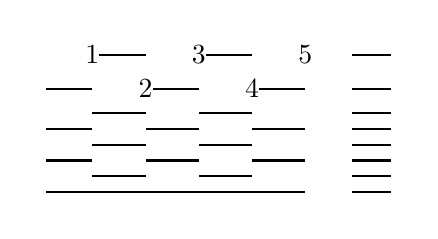
\begin{tikzpicture}
        \node[scale=1]{
        \begin{quantikz}
            \qw &\bgbs{1}& \qw     &\bgbs{3}& \qw     & \bgbs{5}& \agb & \qw\\[-0.3cm]
            \qw & \qw    & \bgbs{2}& \qw    & \bgbs{4}& \qw     & \agb & \qw\\[-0.3cm]
            \qw & \bgb   & \qw     & \bgb   & \qw     & \bgb    & \agb & \qw\\[-0.3cm]
            \qw & \qw    & \bgb    & \qw    & \bgb    & \qw     & \agb & \qw\\[-0.3cm]
            \qw & \bgb   & \qw     & \bgb   & \qw     & \bgb    & \agb & \qw\\[-0.3cm]
            \qw & \qw    & \bgb    & \qw    & \bgb    & \qw     & \agb & \qw\\[-0.3cm]
            \qw & \bgb   & \qw     & \bgb   & \qw     & \bgb    & \agb & \qw\\[-0.3cm]
            \qw & \qw    & \qw     & \qw    & \qw     & \qw     & \agb & \qw
        \end{quantikz}
        };
    \end{tikzpicture}
    \caption{青いゲートブロックは入力回路の Alternating Layered Ansatz(8量子ビット、5層の場合)を表す。赤いゲートブロックは学習回路の Tensor Product Ansatz を表す。}
    \label{fig:alt-tpa-structure}
\end{figure}

% \begin{figure}[H]
%     \begin{minipage}[b]{0.5\columnwidth}
%         \centering
%         \includegraphics[width=8cm]{alt.jpg}
%         \caption{ALT}
%     \end{minipage}
%     \hspace{0\columnwidth}
%     \begin{minipage}[b]{0.5\columnwidth}
%         \centering
%         \includegraphics[width=8cm,height=5cm]{mps.jpg}
%         \caption{MPS}
%     \end{minipage}
% \end{figure}

\ref{sec:qml-upper-var}~節で見たように、$\Var_{V(\bs{\th})}[\pd_\nu \calL(\bs{\th})]$ の上界は次のように与えられる。
\begin{align*}
    \Var_{V(\bs{\th})}[\pd_\nu \calL(\bs{\th})]
    &\leq
    2\max_{i,\bs{\th}} [(\pd_{\ell_i(\bs{\th})}f)^2]
    \times r_{n,s} \times
    \int_{U\in\bbU} dU D_{\HS} (\rho^{(h)} , \bbid/2^s)
\end{align*}

学習回路とオブザーバブルは、命題~\ref{prop:qml-var-local-2-design}の仮定と同じであるとする。すなわち、学習回路は図~\ref{fig:alt-tpa-structure}の赤いゲートブロックの構造を持ち、各 $s=1$ 量子ビット上のゲートブロックはユニタリ $2$--デザインを成すとする。また、コスト関数は次で与えられるとする。
\begin{align*}
    \calL(\bs{\th}) = \frac1N \sum_{i=1}^N (\ell_i(\bs{\th}) - y_i)^2, \quad
    \ell_i(\bs{\th}) = \Tr[\rho_i(\bs{\th}) O_\rmL], \quad
    O_\rmL = \frac{1}{n} \sum_{j=1}^{n}\dyad{0}_{j} \otimes \bbid_{\bar{j}}
\end{align*}
ただし、$y_i \in \{0,1\},\; \ell_i(\bs{\th}) \in [0,1]$ である。
このとき、$2\max_{i,\bs{\th}} [(\pd_{\ell_i(\bs{\th})}f)^2] = 8$, $r_{n,s} = \frac{s\cdot 2^{3(s-1)}}{n^2(2^{2s}-1)^2}$ となる。残る項 $\int_{U\in\bbU} dU D_{\HS} (\rho^{(h)} , \bbid/2^s)$ はデータセットと入力回路の構造に依存するため、これ評価することで、上界のスケーリングが分かる。


$\int_{U\in\bbU} dU D_{\HS} (\rho^{(h)} , \bbid/2^s)$ を入力回路がローカルユニタリ $2$--デザインを成すという仮定の下で、各量子ビット数 $n$、入力回路の各層数 $L$ に対して、上界を計算しプロットしたものが図~\ref{fig:qml-var-alt}の右である\footnote{ここでは Random Tensor Network Integrator (RTNI)~\cite{fukuda2019rtni}を用いて、シンボリックな計算を行った。具体的な計算方法については、補足の\ref{sec:alt-calculation}節に示す。}。破線は Alternating Layered Ansatz の回路を十分深くした場合の収束先、つまり、\ref{sec:haar-random-input}節で得たグローバルユニタリ $2$--デザインの場合の結果 $\calD_{\Haar} = \frac{2^s - 2^{-s}}{2^n + 1}$ である(図~\ref{fig:qml-var-alt}の左における破線もこれと同じである)。
% Matrix Product State (MPS) の図も同様である。

さらに、同様の設定の下、量子回路シミュレーション(測定回数 $\infty$)によって、アヤメのデータセットの分類問題\footnote{用いたアヤメのデータセットは4つの特徴量と2つのラベルからなり、それぞれのラベルに対応するサンプル数は50である。}におけるコスト関数の勾配の分散を計算した。その結果が、図~\ref{fig:qml-var-alt}の左である。
図~\ref{fig:qml-var-alt}の左右を比較すると、確かに右のプロットは上界として機能していることがわかる。

ただし、Alternating Layered Ansatz のゲートブロックには図~\ref{fig:alt-example}の構造を用いた。
また、学習回路は図~\ref{fig:tpa-example}の Tensor Product Ansatz を用い、深さを $10$ 層とした。
$10$ 層は各量子ビットがユニタリ $2$--デザインを成すのに十分な層数である。
これは、図~\ref{fig:1qubit-tpa-exp}において、1量子ビットで10 層の Tensor Product Ansatz のフレームポテンシャルが、ユニタリ $2$--デザインのフレームポテンシャルに十分に収束していることからわかる(サンプル数は $2\times10^4$)。よって、$10$ 層あれば、各量子ビットがローカルユニタリ $2$--デザインを成すとみなせる。

また、図~\ref{fig:qml-var-alt}の左の勾配の分散の計算のために、全てのパラメーターを $10$ 回ランダムにサンプリングした。そして、プロットしたのは、学習回路の各パラメーターに関する勾配の分散 $\Var[\pd_{\th_i} \calL(\bs{\th})]$ を $i$ について平均したものである。

\begin{figure}[H]
    \centering
    \begin{tikzpicture}
        \node[scale=1]{
            \begin{quantikz}
                \qw & \gate[wires=2,style={fill=cyan!50}][1cm]{}& \qw\\
                \qw & \qw                  & \qw
            \end{quantikz}
            \begin{quantikz}
                {\LARGE \textbf{=}}
            \end{quantikz}
            \begin{quantikz}
                \qw & \gate{R_x}&\gate{R_y}&\ctrl{1}& \qw\\
                \qw & \gate{R_x}&\gate{R_y}&\targ{} & \qw
            \end{quantikz}
            };
    \end{tikzpicture}
    \caption{ALT のゲートブロックとして用いた構造}
    \label{fig:alt-example}
\end{figure}

\begin{figure}[H]
    \centering
    \begin{tikzpicture}
        \node[scale=1]{
            \begin{quantikz}
                \qw & \gate[wires=1,style={fill=red!30}][1cm][0.7cm]{}& \qw
            \end{quantikz}
            \begin{quantikz}
                {\LARGE \textbf{=}}
            \end{quantikz}
            \begin{quantikz}
                \qw\slice{} & \gate{R_x} &\gate{R_y}\slice{$\times 10$} & \qw
            \end{quantikz}
            };
    \end{tikzpicture}
    \caption{TPA のゲートブロックとして用いた構造}
    \label{fig:tpa-example}
\end{figure}

\begin{figure}[H]
    \centering
    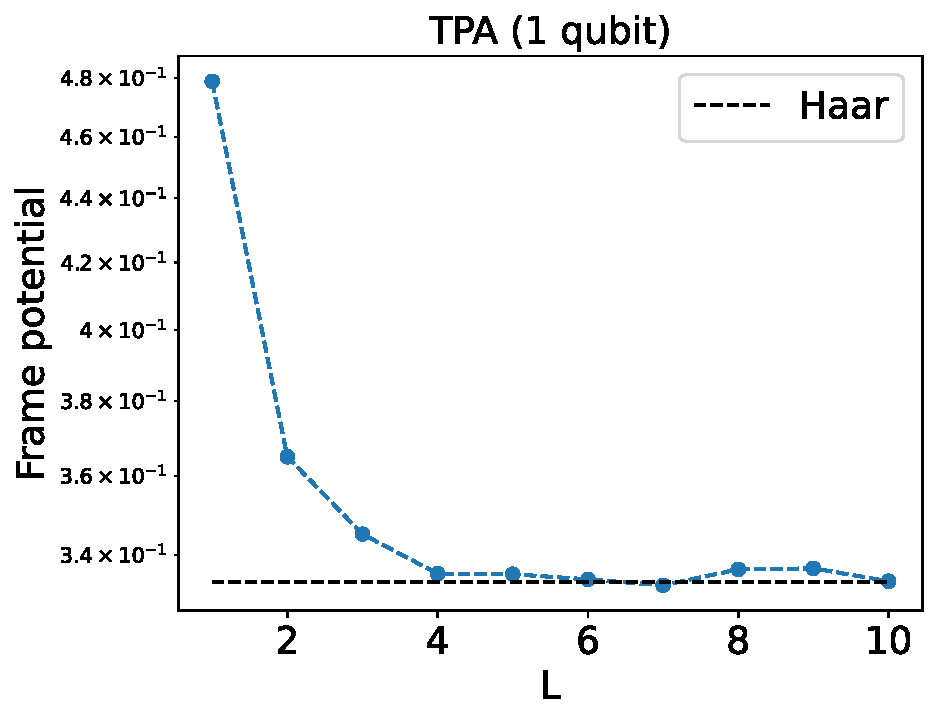
\includegraphics[width=9cm]{1qubit-tpa-exp.pdf}
    \caption{1量子ビットの Tensor Product Ansatz のフレームポテンシャル。黒の破線は量子回路がユニタリ $2$--デザインを成す場合のフレームポテンシャル($=1/3$)である。}
    \label{fig:1qubit-tpa-exp}
\end{figure}


\begin{figure}[H]
    \begin{minipage}[b]{0.5\columnwidth}
        \centering
        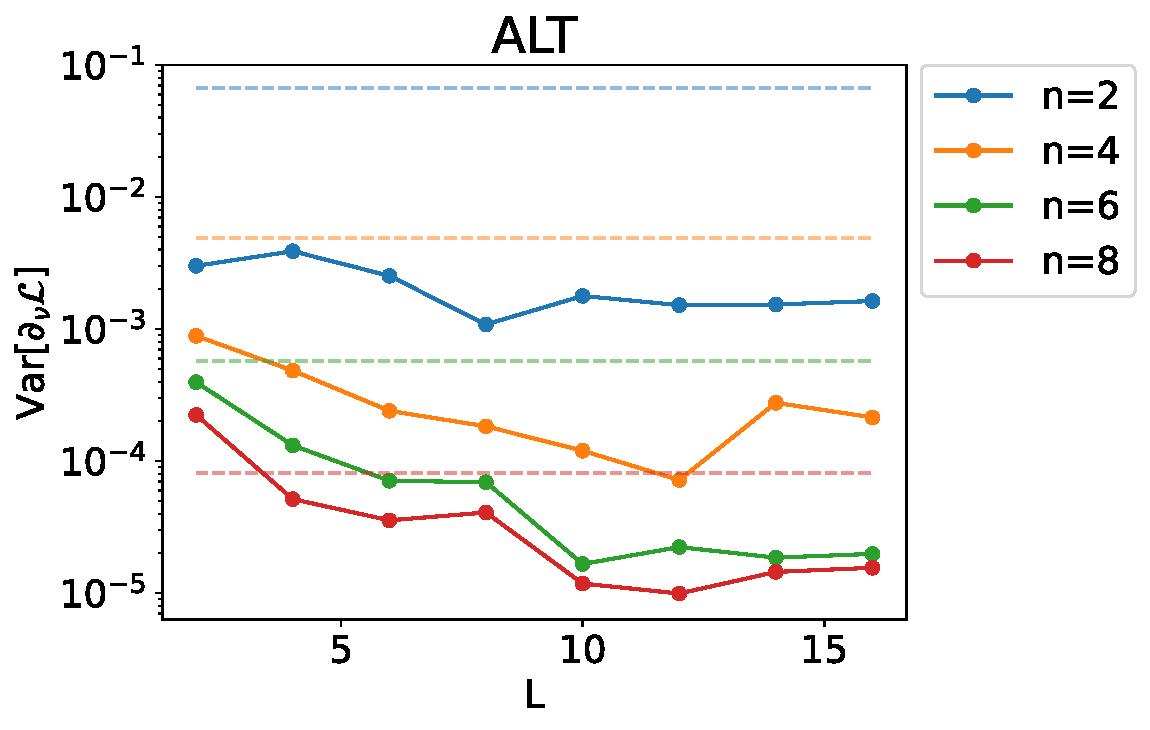
\includegraphics[width=8.5cm]{qml-var-alt.pdf}
    \end{minipage}
    \hspace{0\columnwidth}
    \begin{minipage}[b]{0.5\columnwidth}
        \centering
        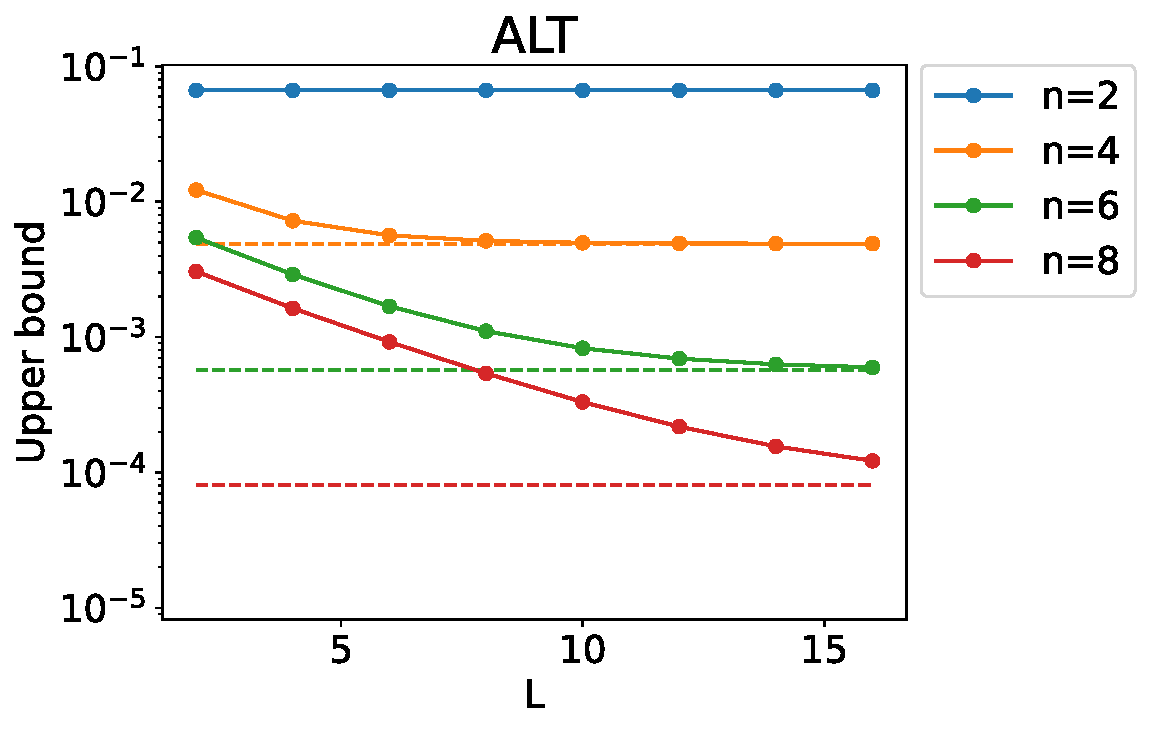
\includegraphics[width=8.5cm]{qml-var-bound-alt.pdf}
    \end{minipage}
    \caption{入力回路に ALT を用いた場合のコスト関数の勾配の分散(左)とその上界(右)}
    \label{fig:qml-var-alt}
\end{figure}

我々は、特にデータの入力が勾配の分散に与える影響に興味があった。
そこで、上界の表式のうちデータ入力に依存する項 $\int_{U\in\bbU} dU D_{\HS} (\rho^{(h)} , \bbid/2^s)$ だけに着目してプロットすると、図~\ref{fig:hsd-alt-analytical}のようになる。  

解析的には示せていないが、図から曲線はある直線 $\beta^{-L}\,(1 < \ex\beta)$ を下回らないことが分かる。よって、上界が量子ビット数 $n$ に対して指数関数的に落ちないためには、ある $\gamma$ に対して $n^{-\gamma} < \beta^{-L}$、すなわち、$L < \gamma\log{n}/\log\beta$ である必要がある。これが、入力回路に Alternating Layered Ansatz を用いた場合に、バレンプラトーが起きないための必要条件である。
以上から、バレンプラトーが起きないためには学習回路が浅いことに加えて、入力回路も $\order{\log{n}}$ 程度に浅くなければならないことが分かる。

\begin{figure}[H]
    \centering
    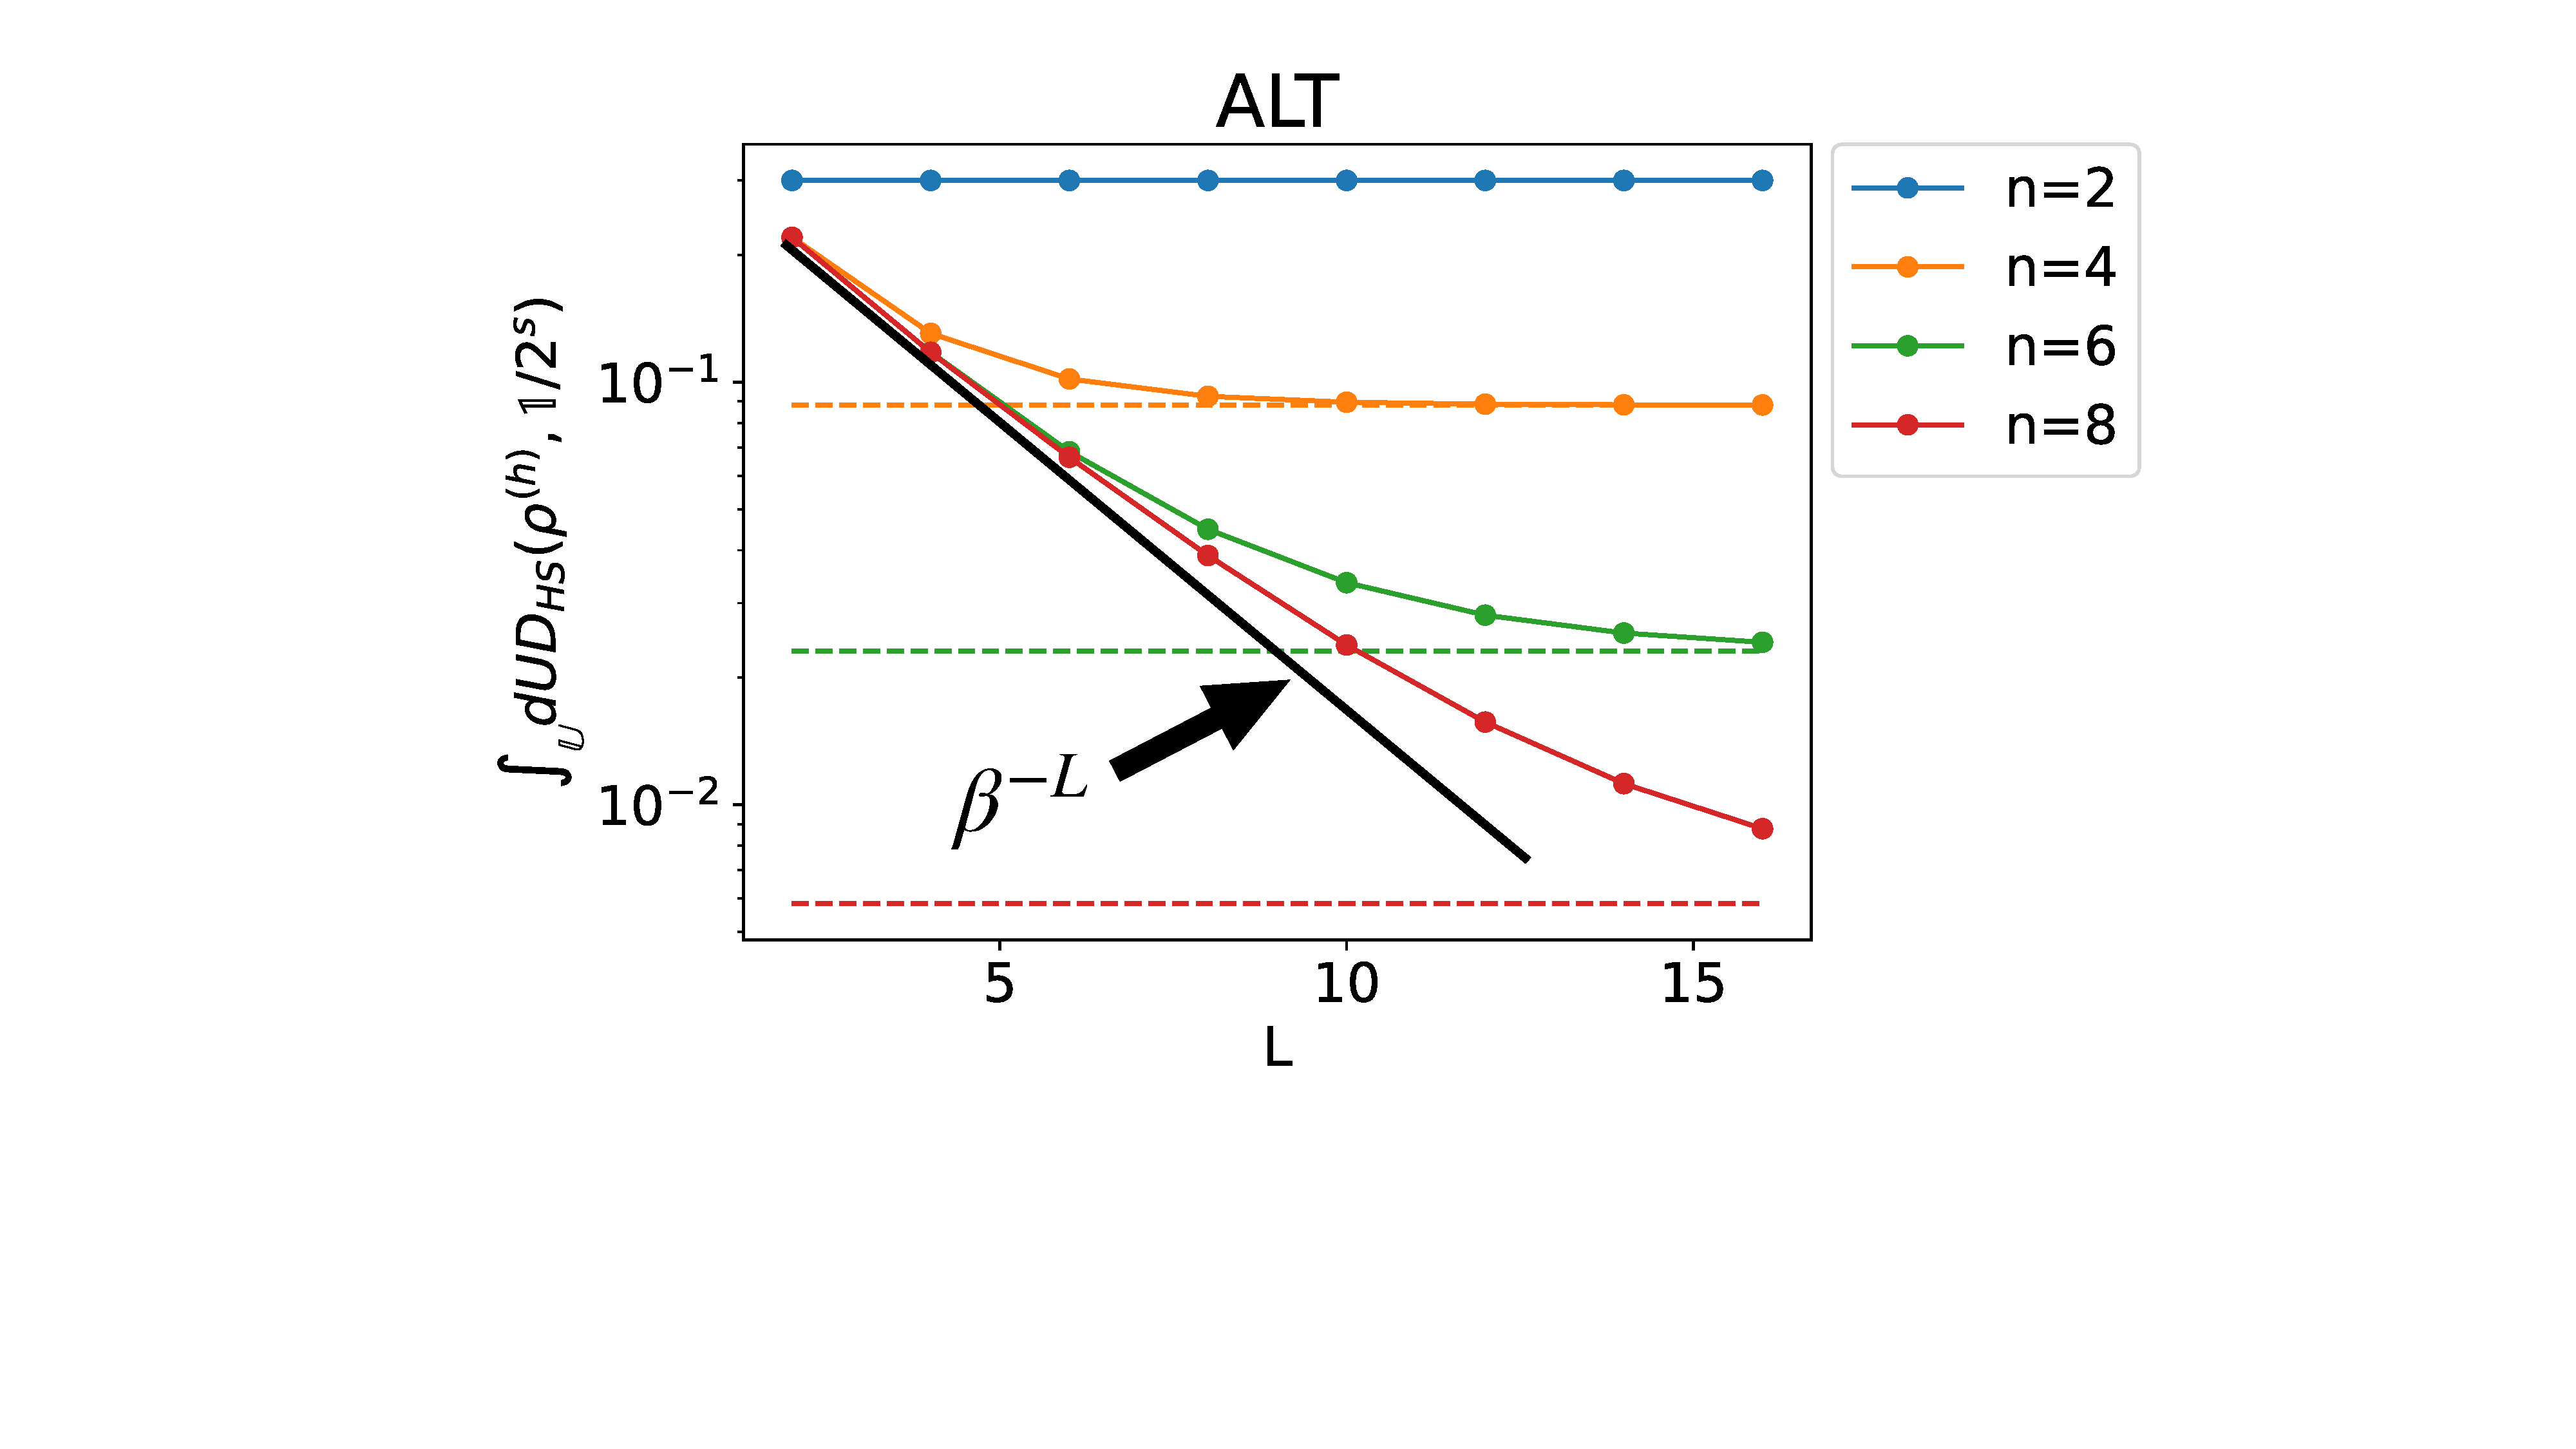
\includegraphics[width=11cm]{hsd-alt-analytical-with-line.pdf}
    \caption{入力回路に ALT を用いた時の $\int_{U\in\bbU} dU D_{\HS} (\rho^{(h)} , \bbid/2^s)$ の計算結果}
    \label{fig:hsd-alt-analytical}
\end{figure}


\section{ノイズの影響}\label{sec:qml-var-noise}
ここまでのコスト関数の勾配の分散の計算においては、ノイズは考慮していなかった。しかし、実際の量子コンピューターにはノイズが存在し、ノイズはバレンプラトーの原因の1つでもある。そこで、ノイズの影響も考慮した場合に、コスト関数の勾配の分散の上界がどのように変化するかを調べる。具体的には、\ref{sec:qml-var-local-2-design}~節で行った計算に Depolarizing ノイズを仮定して、コスト関数の勾配の分散の上界を計算する。
各層のユニタリチャネル $\calE_i(\rho) = U_i\rho U_i\dg,\, i = 1,\,2,\,\cdots,\,L$ に付随して、次の Depolarizing noise channel $\calN_p$ を作用させることを考える。
\begin{align*}
    \calN_p(\rho) = (1-p)\rho + \frac{p}{d}\,\bbid
\end{align*}

このとき、全体のチャネル $\calN = \bigcirc_{i=1}^L \calN_{p} \circ \calE_i$ は次のように表されることを既に確認した(\ref{sec:depolarizing-channel}~節)。
\begin{align*}
    \calN(\rho)
    = (1 - p)^L\calE(\rho) + \{1 - (1 - p)^L\}\,\frac{\bbid}{2^n}
\end{align*}
ただし、$\calE := \bigcirc_{i=1}^L \calE_i$ である。

$D_{HS}(\rho,\,\bbid/d) = \Tr[\rho^2] - \frac{1}{d}$ であることを用いると、
\begin{align}
    D_{HS}(\calN(\rho),\,\bbid/d)
    &= \Tr[\calN(\rho)^2] - \frac{1}{d}\nonumber\\
    &= (1-p)^L\qty{(1-p)^L\Tr[\rho^2] - \frac{1}{d}}\nonumber\\
    &\leq (1-p)^L\qty{\Tr[\rho^2] - \frac{1}{d}}\nonumber\\
    &= (1-p)^L\,D_{HS}(\rho,\,\bbid/d).
\end{align}

したがって、ノイズの影響を考慮した場合のコスト関数の勾配の分散の上界は、次のようになる。
\begin{align}
    \Var_{V(\bs{\th})}[\pd_\nu \calL_{\text{noise}}(\bs{\th})]
    &\leq
    2\max_{i,\bs{\th}} [(\pd_{\ell_i(\bs{\th})}f)^2]
    \times r_{n,s} \times
    \int_{U\in\bbU} dU D_{\HS} (\calN(\rho^{(h)}) , \bbid/2^s)\nonumber\\
    &\leq
    2\max_{i,\bs{\th}} [(\pd_{\ell_i(\bs{\th})}f)^2]
    \times r_{n,s} \times
    (1-p)^L\int_{U\in\bbU} dU D_{\HS} (\rho^{(h)} , \bbid/2^s)\label{eq:qml-var-bound-noise}
\end{align}

図~\ref{fig:qml-var-alt}の右はノイズがある場合の上界\eqref{eq:qml-var-bound-noise}をプロットしたものである。
また、\ref{sec:qml-var-local-2-design}~節と同じ設定の下、Depolarizing ノイズ ($p=0.03$)を加えてアヤメの分類問題のコスト関数の勾配の分散を計算すると、図~\ref{fig:qml-var-alt-noise}の左のようになった。
勾配の分散の計算のために、全てのパラメーターを $10$ 回ランダムにサンプリングした。ただし、プロットしたのは、学習回路の各パラメーターに関する勾配の分散 $\Var[\pd_{\th_i} \calL(\bs{\th})]$ を $i$ について平均したものである。
図~\ref{fig:qml-var-alt}と比較すると、コスト関数の勾配の分散がさらに小さくなっていることが分かる。
上界のノイズに依る項 $(1-p)^L$ だけを見ても、バレンプラトーが起きないためには $L \in \order{\log{n}}$ でなければならないことが分かる。
\begin{figure}[H]
    \begin{minipage}[b]{0.5\columnwidth}
        \centering
        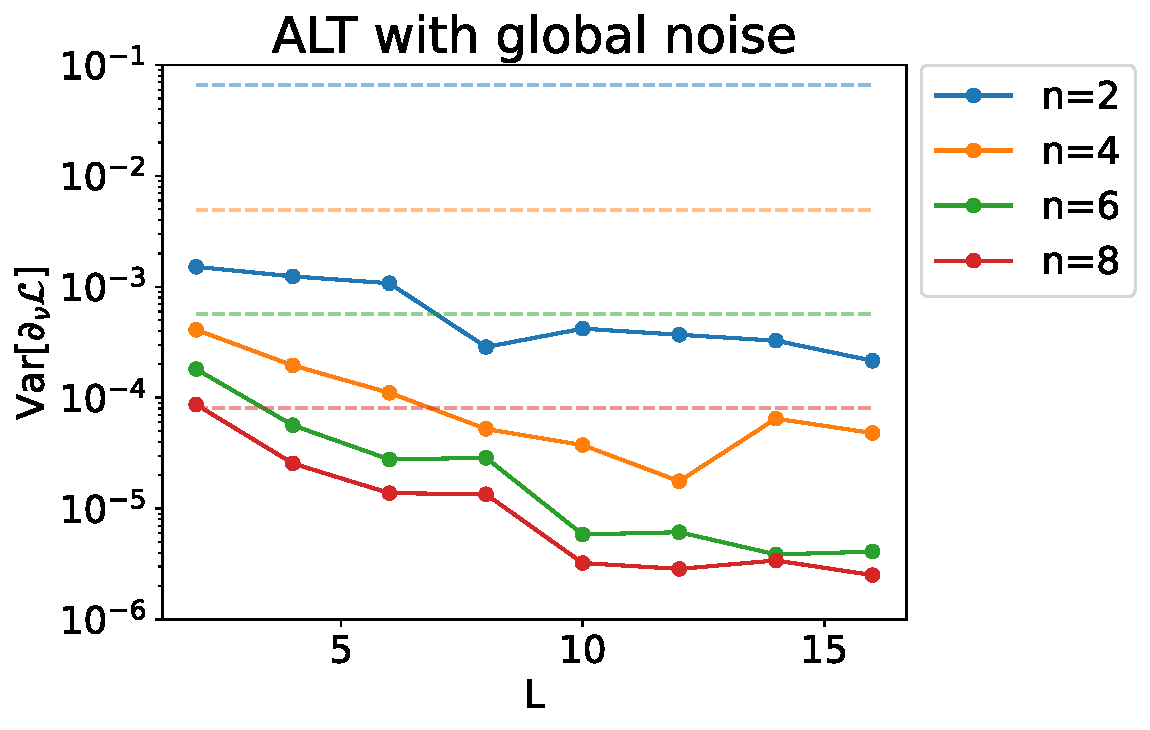
\includegraphics[width=8.5cm]{alt-var_global-noise.pdf}
        % \caption{ALT:ノイズなしのコスト関数の勾配の分散}
    \end{minipage}
    \hspace{0\columnwidth}
    \begin{minipage}[b]{0.5\columnwidth}
        \centering
        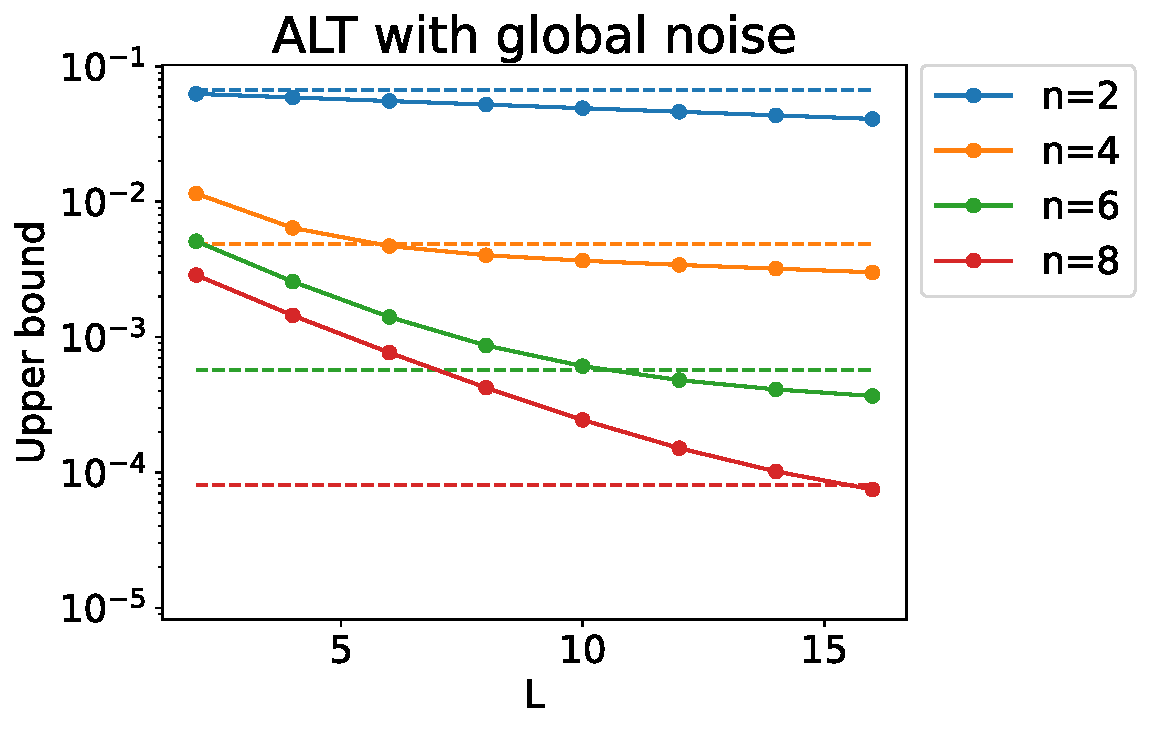
\includegraphics[width=8.5cm]{alt-var-bound_global-noise.pdf}
    \end{minipage}
    \caption{ノイズのある入力回路に ALT を用いた場合のコスト関数の勾配の分散(左)とその上界(右)}
    \label{fig:qml-var-alt-noise}
\end{figure}

\newpage
\chapter{量子機械学習におけるコスト関数の勾配の分散の下界}\label{chap:lower-bound}
この章では、コスト関数の勾配の分散の下界のスケーリングについて調べる。
\ref{sec:cost1}~節では、入力データがガウス分布に従うという仮定の下、絶対誤差のコスト関数 $\calL_{\mathrm{MAE}}(\bs{\th}) = \frac1N\sum_{i=1}^N \;|\ell_i(\bs{\th}) - y_i|$ の勾配の分散の下界を計算する。
\ref{sec:cost2}~節では、二乗誤差のコスト関数 $\calL_{\mathrm{MSE}}(\bs{\th}) = \frac1N\sum_{i=1}^N \;\qty(\ell_i(\bs{\th}) - y_i)^2$ や交差エントロピー誤差のコスト関数 $\calL_{\mathrm{LOG}}(\bs{\th}) = \frac1N\sum_{i=1}^N \;[-y_i\log\ell_i(\bs{\th}) - (1-y_i)\log(1-\ell_i(\bs{\th}))]$ の勾配の分散を、絶対誤差のコスト関数の勾配の分散から推定する。

\section{絶対誤差のコスト関数の勾配の分散}\label{sec:cost1}
この節では、量子回路の構造は図~\ref{fig:circuit-setting}で与えられるものとする。すなわち、学習回路は $\xi$ 個の $s$ 量子ビットユニタリからなり、全量子ビット数は $n=s\times\xi$ である。
そして、2値分類 $y_i \in \{0,1\}$ の問題設定において、絶対誤差のコスト関数の勾配の分散の下界を計算する。

コスト関数が 
$$
    \calL_{\mathrm{MAE}}(\bs{\th}) = \frac1N\sum_{i=1}^N \,|\ell_i(\bs{\th}) - y_i|,\quad \ell_i(\bs{\th}) = \Tr[\rho_i(\bs{\th})\,O_\rmL],\quad O_\rmL = \frac{1}{n} \sum_{j=1}^{n}\dyad{0}_{j} \otimes \bbid_{\bar{j}}
$$
で与えられるとき、コスト関数の勾配は、 $\pd_\nu := \pd/\pd\th_\nu$, $w_i := \sgn(\ell_i(\bs{\th}) - y_i)$ として、
\begin{align}
    \pd_\nu\calL_{\mathrm{MAE}}(\bs{\th})
    &= \frac1N\sum_{i=1}^N \;w_i \cdot \pd_\nu\ell_i(\bs{\th})
\end{align}
と表せる。
ただし、$\ell_i(\bs{\th}) \in [0,1]$ であることから $w_i$ と $y_i$ は次のように対応する。
\begin{align}
    w_i =
    \begin{cases}
        \;\;\,1 & \text{if}\quad y_i = 0\\
             -1 & \text{if}\quad y_i = 1
    \end{cases}
\end{align}

ここで、学習回路の各 $s$ 量子ビットユニタリがユニタリ $2$--デザインを成すと仮定する。また、証明\ref{proof:qml-upper-var}で示したように、勾配の平均は $0$ である。よって、勾配の分散は次のように計算できる。
\begin{align}
    \Var_{V(\bs{\th})}[\pd_\nu\calL_{\mathrm{MAE}}(\bs{\th})]
    &= \E_{V(\bs{\th})}[(\pd_\nu\calL_{\mathrm{MAE}}(\bs{\th}))^2]\nonumber\\
    &= \frac{1}{N^2}\sum_{i,j=1}^N\;
    w_i\, w_j
    \E_{V(\bs{\th})}[\pd_\nu\ell_i(\bs{\th})\cdot\pd_\nu\ell_j(\bs{\th})]\label{eq:abs-cost-variance}
\end{align}

$\E_{V(\bs{\th})}[\pd_\nu\ell_i(\bs{\th})\cdot\pd_\nu\ell_j(\bs{\th})]$ は、論文~\cite{cerezo2021cost}の結果を拡張することで次のように計算できる。略証は\ref{sec:prf-covariance}~節を参照。
\begin{screen}
    \begin{corollary}\label{cor:covariance}
        (論文~\cite{cerezo2021cost}の Supplementary Note 5, B の拡張された結果)
        量子回路の構造は図~\ref{fig:circuit-setting}で与えられ、学習回路の各 $s$ 量子ビットユニタリがユニタリ $2$--デザインを成すとき、次の等式が成り立つ。
        \begin{align}
            \E_{V(\bs{\th})}\qty[\pd_\nu\ell_i(\bs{\th})\,\cdot\,\pd_\nu\ell_j(\bs{\th})] = r_{n,s}\qty(\Tr\qty[\rho_i^{(h)}\rho_j^{(h)}]-\frac{1}{2^s}),
            \quad r_{n,s} := \frac{s\,2^{3(s-1)}}{n^2(2^{2s}-1)^2}
        \end{align}
    \end{corollary}
\end{screen}

よって、式~\eqref{eq:abs-cost-variance}は次のように書き換えられる。
\begin{align}\label{eq:abs-cost-variance-2}
    \Var_{V(\bs{\th})}[\pd_\nu\calL_{\mathrm{MAE}}(\bs{\th})]
    &= \frac{r_{n,s}}{N^2}
    \sum_{i,j=1}^N\; w_i\, w_j\,
    \qty(\Tr[\rho_i^{(h)}\rho_j^{(h)}]-\frac{1}{2^s})\\
    &=
    \frac{r_{n,s}}{N^2}
    \qty[
        \sum_{w_i=w_j}^N\;
        \qty(\Tr[\rho_i^{(h)}\rho_j^{(h)}]-\frac{1}{2^s})
        -
        \sum_{w_i\neq w_j}^N\;
        \qty(\Tr[\rho_i^{(h)}\rho_j^{(h)}]-\frac{1}{2^s})
    ]
\end{align}

上の表式から、入力状態に依存する $\Tr[\rho_i^{(h)}\rho_j^{(h)}]$ が重要であり、$\Tr[\rho_i^{(h)}\rho_j^{(h)}]$ が同じラベルの場合と異なるラベルの場合でどのようにスケーリングするかが、勾配の分散に影響することがわかる
\footnote{
論文\cite{garcia-martin2023deep}においては、入力状態が十分に分離していることを、同じラベルの入力状態間のカーネルと異なるラベルの入力状態間のカーネルが次のようにスケールことと述べている。
\begin{alignat*}{2}
    \Tr[\rho_i \rho_{i^{\prime}}] &\in \Omega\qty(\frac{1}{\poly(n)}), \quad&\text{if} \quad y_i=y_{i^{\prime}} \\
    \Tr[\rho_i \rho_{i^{\prime}}] &\in \calO\qty(\frac{1}{2^n}), \quad&\text{if} \quad y_i \neq y_{i^{\prime}}
\end{alignat*}
}。

式\eqref{eq:abs-cost-variance-2}をさらに変形すると、次のようになる。
\begin{align}
    \Var_{V(\bs{\th})}[\pd_\nu\calL_{\mathrm{MAE}}(\bs{\th})]
    &=
    r_{n,s}\;
    \qty(\Tr[(\overline{\rho})^2] - \frac{w^2}{2^s}) \label{eq:abs-cost-variance-3}
\end{align}
ただし、$w := \frac1N\sum_{i=1}^N w_i,\; \overline{\rho} := \frac{1}{N}\sum_{i=1}^N w_i\rho_i^{(h)}$ とした。前者は $w_i = \pm1$ であることに注意すると、$\abs{w} \leq 1$ である。
特に、$\#\{y_i|y_i=0\} = \#\{y_i|y_i=1\} = N/2$ ならば $w = 0$ であり、$\#\{y_i|y_i=0\} = N$ または $\#\{y_i|y_i=1\} = N$ ならば $|w| = 1$ である。
後者は、論文\cite{hubregtsen2022training}において述べられているように Kernel Alignment と類似した量である。簡単のため、$\overline{\rho}$ と表しているが、この量自体は密度演算子とは限らないことに注意する。なぜなら、$\Tr[\overline{\rho}] = w$ だからである。
% また、平均した状態の純粋度 $\Tr[(\bar{\rho})^2]$ はカーネル $\kappa_{FQ}(\bs{x},\bs{y})$ の平均として解釈することができることに言及しておく。
% \footnote{
%     次の変形を行うことができる。
%     \begin{align}
%         \Tr[(\bar{\rho})^2]
%         = \Tr\qty[\qty(\int \rho(\bs{x}_i)\,\mu(d\bs{x}))^2]
%         = \iint\Tr[\rho(\bs{x})\rho(\bs{y})]\mu(d\bs{x})\mu(d\bs{y})
%         =:\iint\kappa_{FQ}(\bs{x},\bs{y})\;\mu(d\bs{x})\mu(d\bs{y})
%     \end{align}
% }


さらに、$\overline{\rho}_\pm := \frac{1}{N}\sum\limits_{i,(w_i=\pm1)} \rho_i^{(h)}$ として、$\overline{\rho}$ を変形すると次のようになる。
\begin{align}
    \Tr[(\overline{\rho})^2]
    =  \Tr[(\overline{\rho}_+ - \overline{\rho}_-)^2]
    = D_{HS}(\overline{\rho}_+,\, \overline{\rho}_-)
\end{align}
したがって、それぞれのラベルの平均入力状態である $\overline{\rho}_+$ と $\overline{\rho}_-$ の差が大きいほど、下界も大きくなることがわかる。



\subsection{下界のスケーリング(1)}\label{sec:lower-bound-1}
ここでは、先行研究~\cite{li2022concentration}で得られた結果を拡張し、コスト関数の勾配の分散の下界を計算する。
入力データの各成分はガウス分布に従い、入力回路は図~\ref{fig:circuit-concentration-1}のように $R_y$ ゲートのみで構成されているとする。
このとき、次の定理が成り立つ。証明は\ref{sec:prf-concentration-1}~節を参照。

\begin{screen}
    \begin{theorem}\label{thm:concentration-1}
        (論文~\cite{li2022concentration}の Theorem 1 の拡張された結果)
        $\calX = \{\bs{x}\}$, $\calZ = \{\bs{z}\}$ はそれぞれラベル $y_i=0$ と $y_i=1$ に属する入力データセットであり、$|\calX|:|\calZ| = p:q\;(p+q=1)$ であるとする。
        そして、各データサンプルを次のように表記する:$\bs{x} = (\bs{x}_{j})_{j=1}^n,\, \bs{x}_{j} = (x_{j,d})_{d=1}^L$, $\bs{z} = (\bs{z}_{j})_{j=1}^n,\, \bs{z}_{j} = (z_{j,d})_{d=1}^L$。異なるラベルに属する入力データを量子回路に同時には入力しないとする。
        入力データの各成分の分布は $x_{j,d} \sim \calN(\mu_{x|j,d}, \sigma_{x|j,d}^2)$, $z_{j,d} \sim \calN(\mu_{z|j,d}, \sigma_{z|j,d}^2)$ であり、分散は $\sigma_{\min} \leq \sigma_{x|\fa j,d},\, \sigma_{z|\fa j,d} \leq \sigma_{\max}$ を満たすとする。また、量子回路は図~\ref{fig:circuit-concentration-1}のように構成されている。ただし、$1\leq j\leq n,\, 1\leq d\leq L$ である。
        このとき、$\bar{\rho} = p\E_\calX[\rho^{(h)}(\bs{x})] - q\E_\calZ[\rho^{(h)}(\bs{z})]$ について次の不等式が成り立つ。
        \begin{align}
            \frac{1}{2^s}
            \qty[w^2 + \sum_{j=1}^s \qty(p\,e^{-\Sigma_{x|j}/2} - q\,e^{-\Sigma_{z|j}/2})^2]
            \leq \Tr[(\bar{\rho})^2]
            \leq \frac{1}{2^s} (1 + e^{-L\,\sigma_{\min}^2})^s
        \end{align}
        ただし、$n,s$ は量子ビット数($n=s\times\xi$)、$L$ は入力回路の層数、$w = p - q$, $\Sigma_{x|j}:=\sum_{d=1}^L \sigma_{x|j,d}^2$, $\Sigma_{z|j}:=\sum_{d=1}^L \sigma_{z|j,d}^2$ である。
    \end{theorem}
\end{screen}
この定理においては、$\th_\nu$ が含まれる $h\,(1\leq h\leq\xi)$ 番目の $s$ 量子ビットについてだけ考えればよいことに注意する。


\newcommand{\bgate}[1]{\gate[wires=1,style={fill=cyan!50}]{#1}}
\newcommand{\rgate}[1]{\gate[wires=4,style={fill=red!30}]{#1}}
\begin{figure}[H]
    \centering
    \begin{tikzpicture}
    \node[scale=0.9]{
        \begin{quantikz}
            \lstick{$\ket{0}$} & \bgate{R_y(x_{1,1})}    & \bgate{R_y(x_{1,2})}    &\ \ldots\ & \bgate{R_y(x_{1,L-1})}    & \bgate{R_y(x_{1,L})}    &\rgate{V_1(\bs{\th}_1)}& \meter{} \\
            \lstick{$\ket{0}$} & \bgate{R_y(x_{2,1})}    & \bgate{R_y(x_{2,2})}    &\ \ldots\ & \bgate{R_y(x_{2,L-1})}    & \bgate{R_y(x_{2,L})}    & \qw                     & \meter{} \\
            \wave&&&&&&&&&\\
            \lstick{$\ket{0}$} & \bgate{R_y(x_{s,1})}    & \bgate{R_y(x_{s,2})}    &\ \ldots\ & \bgate{R_y(x_{s,L-1})}    & \bgate{R_y(x_{s,L})}    & \qw                     & \meter{}\\
            \lstick{$\ket{0}$} & \bgate{R_y(x_{s+1,1})}  & \bgate{R_y(x_{s+1,2})}  &\ \ldots\ & \bgate{R_y(x_{s+1,L-1})}  & \bgate{R_y(x_{s+1,L})}  &\rgate{V_2(\bs{\th}_2)}& \meter{} \\
            \lstick{$\ket{0}$} & \bgate{R_y(x_{s+2,1})}  & \bgate{R_y(x_{s+2,2})}  &\ \ldots\ & \bgate{R_y(x_{s+2,L-1})}  & \bgate{R_y(x_{s+2,L})}  & \qw                     & \meter{} \\
            \wave&&&&&&&&&\\
            \lstick{$\ket{0}$} & \bgate{R_y(x_{2s,1})}   & \bgate{R_y(x_{2s,2})}   &\ \ldots\ & \bgate{R_y(x_{2s,L-1})}   & \bgate{R_y(x_{2s,L})}   & \qw                     & \meter{}\\
            \wave&&&&&&&&&\\
            \lstick{$\ket{0}$} & \bgate{R_y(x_{n-s+1,1})}& \bgate{R_y(x_{n-s+1,2})}&\ \ldots\ & \bgate{R_y(x_{n-s+1,L-1})}& \bgate{R_y(x_{n-s+1,L})}&\rgate{V_\xi(\bs{\th}_\xi)}& \meter{} \\
            \lstick{$\ket{0}$} & \bgate{R_y(x_{n-s+2,1})}& \bgate{R_y(x_{n-s+2,2})}&\ \ldots\ & \bgate{R_y(x_{n-s+2,L-1})}& \bgate{R_y(x_{n-s+2,L})}& \qw                     & \meter{} \\
            \wave&&&&&&&&&\\
            \lstick{$\ket{0}$} & \bgate{R_y(x_{n,1})}    & \bgate{R_y(x_{n,2})}    &\ \ldots\ & \bgate{R_y(x_{n,L-1})}    & \bgate{R_y(x_{n,L})}    & \qw                     & \meter{}
        \end{quantikz}};
    \end{tikzpicture}
    \caption{$n = s\times\xi$ 量子ビットからなる量子回路。入力回路は $L$ 層の $R_y$ ゲートからなる。学習回路は $\xi$ 個の $s$ 量子ビットユニタリからなる。}
    \label{fig:circuit-concentration-1}
\end{figure}


定理~\ref{thm:concentration-1}と式~\eqref{eq:abs-cost-variance-3}より、直ちに次の定理が導かれる。
\begin{screen}
    \begin{theorem}\label{thm:lower-bound-1}
        系\ref{cor:covariance}と定理\ref{thm:concentration-1}の条件のもとで、
        絶対誤差のコスト関数の勾配の分散は上下から次のように抑えられる。
        \begin{align}
            \frac{r_{n,s}}{2^s}\;
            \sum_{j=1}^s \qty(p\,e^{-\Sigma_{x|j}/2} - q\,e^{-\Sigma_{z|j}/2})^2
            \leq \Var_{V(\bs{\th})}[\pd_\nu\calL_{\mathrm{MAE}}(\bs{\th})]
            \leq \frac{r_{n,s}}{2^s}\;\qty[\qty(1 + e^{-L\,\sigma_{\min}^2})^s - w^2]
        \end{align}
        ただし、$r_{n,s} := \frac{s\,2^{3(s-1)}}{n^2(2^{2s}-1)^2}$, $w = p - q$ である。
    \end{theorem}
\end{screen}

\subsubsection{$|\calX|:|\calZ| = 1:1$ の場合}
$|\calX|:|\calZ| = 1:1 \iff p = q = 1/2,\, w = 0$ の場合、定理\ref{thm:lower-bound-1}は次のようになる。
\begin{align}
    \frac{r_{n,s}}{2^{s+2}}\;
    \sum_{j=1}^s
    \qty(e^{-\Sigma_{x|j}/2}- e^{-\Sigma_{z|j}/2})^2
    \leq \Var_{V(\bs{\th})}[\pd_\nu\calL_{\mathrm{MAE}}(\bs{\th})]
    \leq r_{n,s}\;\qty(\frac{1 + e^{-L\,\sigma_{\min}^2}}{2^s})^s
    \leq r_{n,s}
\end{align}

これより $e^{-\Sigma_{x|j}/2},\,e^{-\Sigma_{z|j}/2}$ の差が大きいほど、下界が大きくなることがわかる。しかし、$(e^{-\Sigma_{x|j}/2}- e^{-\Sigma_{z|j}/2})^2$ は層数 $L$ を増やすと指数関数的に小さくなる。
また、すべての $j$ について $e^{-\Sigma_{x|j}/2} = e^{-\Sigma_{z|j}/2}$ である場合、下界は $0$ となり意味をなさない\footnote{極端な例として、$\calX = \calZ$ の場合は、$\calL_{\mathrm{MAE}}(\bs{\th}) = 1/2$ となるため、勾配は $0$、したがって勾配の分散も $0$ となる。ゆえに、下界が $0$ となることもあり得る。}。

一方で、$s \in \order{\poly(n)}$ ならば、上界は指数関数的に減少するため、バレンプラトーとなることがわかる。

\subsubsection{$|\calX|:|\calZ| = 1:0$ の場合}
異常検知などに用いられる One class classification~\cite{khan2014oneclass}の場合は、$|\calX|:|\calZ| = 1:0 \iff p = 1,\, q = 0,\, w = 1$ となる。このとき、定理\ref{thm:lower-bound-1}は次のようになる。
\begin{align*}
    &\frac{r_{n,s}}{2^s}\;
    \sum_{j=1}^s e^{-\Sigma_{x|j}}
    \leq \Var_{V(\bs{\th})}[\pd_\nu\calL_{\mathrm{MAE}}(\bs{\th})]
    \leq \frac{r_{n,s}}{2^s}\;\qty[\qty(1 + e^{-L\,\sigma_{\min}^2})^s - 1]
\end{align*}

$\Sigma_{x|j} \leq L\,\sigma_{\max}^2$ であるから、$se^{-L\,\sigma_{\max}^2} \leq \sum_{j=1}^s e^{-\Sigma_{x|j}}$ が成り立つ。
これと、$[(1 + e^{-L\,\sigma_{\min}^2})^s - 1]/2^s \leq 1$ であることから、定理\ref{thm:lower-bound-1}は次のようになる。
\begin{align}
    &\frac{r_{n,s} s}{2^s}\;e^{-L\,\sigma_{\max}^2}
    \leq \Var_{V(\bs{\th})}[\pd_\nu\calL_{\mathrm{MAE}}(\bs{\th})]
    \leq r_{n,s}
\end{align}

$s$ と $\sigma_{\max}^2$ が固定されているとすると、勾配の分散の下界が量子ビット数 $n$ に関して $\order{1/\poly(n)}$ でスケールするためには、$L \in \order{\log{n}}$ でなければならない。
ところで、\ref{sec:quantum-kernel}節の量子カーネル法の説明で述べた Bandwidth というハイパーパラメーターを導入すれば、入力するデータの分散を調整することができる。よって分散の最大値が $\sigma_{\max}^2 \in \order{\log{n}}/L$ を満たすように Bandwidth を調整すれば、$L\,\sigma_{\max}^2 \in \order{\log{n}}$ となるようにできる。しかし、この手法によってバレンプラトーが回避できても、汎化性能に悪影響を及ぼす可能性があることに注意する。

一方、上界については $s \in \order{\poly(n)}$ のとき、上界は指数関数的に減少するため、バレンプラトーとなることがわかる。


\subsection{下界のスケーリング(2)}
ここでも先程と同様に、先行研究~\cite{li2022concentration}で得られた結果を拡張し、コスト関数の勾配の分散の下界を計算する。
ただし、この節では $p = 1,\, q = 0$ である場合のみを考える。
入力データの各成分はガウス分布に従い、入力回路は図~\ref{fig:circuit-concentration-2}のように構成されているとする。
このとき、次の定理が成り立つ。略証は\ref{sec:prf-concentration-2}~節を参照。
\begin{screen}
    \begin{theorem}\label{thm:concentration-2}
        (論文~\cite{li2022concentration}の Theorem 2 の拡張された結果)
        $\calX = \{\bs{x}\}$ はラベル $y_i=0$ に属する入力データセットであるとする。
        そして、各データサンプルを次のように表記する:$\bs{x} = (\bs{x}_{j})_{j=1}^n,\, \bs{x}_{j} = (\bs{x}_{j,d})_{d=1}^L,\,\bs{x}_{j,d} = (x_{j,d,1},x_{j,d,2},x_{j,d,3})$。
        入力データの各成分の分布は $x_{j,d,k} \sim \calN(\mu_{x|j,d,k}, \sigma_{x|j,d,k}^2)$ であり、分散は $\sigma_{\min} \leq \sigma_{x|\fa j,d,k} \leq \sigma_{\max}$ を満たすとする。また、量子回路は図~\ref{fig:circuit-concentration-2}のように構成されている。ただし、$1\leq j\leq n,\, 1\leq d\leq L,\,1\leq k\leq 3$ である。
        このとき、$\bar{\rho} := \E_\calX[\rho^{(h)}(\bs{x})]$ について次の不等式が成り立つ。
        \begin{align}
            \frac{1}{2^s} + e^{-3s\,L\,\sigma_{\max}^2}
            \leq \Tr[(\bar{\rho})^2]
            \leq \frac{1}{2^s} + e^{-L\,\sigma_{\min}^2}
        \end{align}
        ただし、$n,s$ は量子ビット数($n=s\times\xi$)、$L$ は入力回路の層数である。
    \end{theorem}
\end{screen}
この定理においては、$\th_\nu$ が含まれる $h\,(1\leq h\leq\xi)$ 番目の $s$ 量子ビットについてだけ考えればよいことに注意する。


\newcommand{\bbgate}[1]{\gate[wires=4,style={fill=cyan!50}]{#1}}
\begin{figure}
    \centering
    \begin{tikzpicture}
    \node[scale=0.7]{
        \begin{quantikz}
            \lstick{$\ket{0}$} & \bgate{U_3(\bs{x}_{1,1})}    &\bbgate{Etg_{1,1}}& \bgate{U_3(\bs{x}_{1,2})}    &\bbgate{Etg_{1,2}}&\ \ldots\ & \bgate{U_3(\bs{x}_{1,L-1})}    &\bbgate{Etg_{1,L-1}}& \bgate{U_3(\bs{x}_{1,L})}    &\rgate{V_1(\bs{\th}_1)}& \meter{} \\
            \lstick{$\ket{0}$} & \bgate{U_3(\bs{x}_{2,1})}    & \qw           & \bgate{U_3(\bs{x}_{2,2})}    & \qw           &\ \ldots\ & \bgate{U_3(\bs{x}_{2,L-1})}    & \qw               & \bgate{U_3(\bs{x}_{2,L})}    & \qw                     & \meter{} \\
            \wave&&&&&&&&&&\\
            \lstick{$\ket{0}$} & \bgate{U_3(\bs{x}_{s,1})}    & \qw           & \bgate{U_3(\bs{x}_{s,2})}    & \qw           &\ \ldots\ & \bgate{U_3(\bs{x}_{s,L-1})}    & \qw               & \bgate{U_3(\bs{x}_{s,L})}    & \qw                     & \meter{}\\
            \lstick{$\ket{0}$} & \bgate{U_3(\bs{x}_{s+1,1})}  &\bbgate{Etg_{2,1}}& \bgate{U_3(\bs{x}_{s+1,2})}  &\bbgate{Etg_{2,2}}&\ \ldots\ & \bgate{U_3(\bs{x}_{s+1,L-1})}  &\bbgate{Etg_{2.L-1}}& \bgate{U_3(\bs{x}_{s+1,L})}  &\rgate{V_2(\bs{\th}_2)}& \meter{} \\
            \lstick{$\ket{0}$} & \bgate{U_3(\bs{x}_{s+2,1})}  & \qw           & \bgate{U_3(\bs{x}_{s+2,2})}  & \qw           &\ \ldots\ & \bgate{U_3(\bs{x}_{s+2,L-1})}  & \qw               & \bgate{U_3(\bs{x}_{s+2,L})}  & \qw                     & \meter{} \\
            \wave&&&&&&&&&&\\
            \lstick{$\ket{0}$} & \bgate{U_3(\bs{x}_{2s,1})}   & \qw           & \bgate{U_3(\bs{x}_{2s,2})}   & \qw           &\ \ldots\ & \bgate{U_3(\bs{x}_{2s,L-1})}   & \qw               & \bgate{U_3(\bs{x}_{2s,L})}   & \qw                     & \meter{}\\
            \wave&&&&&&&&&&\\
            \lstick{$\ket{0}$} & \bgate{U_3(\bs{x}_{n-s+1,1})}&\bbgate{Etg_{\xi,1}}& \bgate{U_3(\bs{x}_{n-s+1,2})}&\bbgate{Etg_{\xi,2}}&\ \ldots\ & \bgate{U_3(\bs{x}_{n-s+1,L-1})}&\bbgate{Etg_{\xi,L-1}}& \bgate{U_3(\bs{x}_{n-s+1,L})}&\rgate{V_\xi(\bs{\th}_\xi)}& \meter{} \\
            \lstick{$\ket{0}$} & \bgate{U_3(\bs{x}_{n-s+2,1})}& \qw           & \bgate{U_3(\bs{x}_{n-s+2,2})}& \qw           &\ \ldots\ & \bgate{U_3(\bs{x}_{n-s+2,L-1})}& \qw               & \bgate{U_3(\bs{x}_{n-s+2,L})}& \qw                     & \meter{} \\
            \wave&&&&&&&&&&\\
            \lstick{$\ket{0}$} & \bgate{U_3(\bs{x}_{n,1})}    & \qw           & \bgate{U_3(\bs{x}_{n,2})}    & \qw           &\ \ldots\ & \bgate{U_3(\bs{x}_{n,L-1})}    & \qw               & \bgate{U_3(\bs{x}_{n,L})}    & \qw                     & \meter{}
        \end{quantikz}};
    \end{tikzpicture}
    \caption{$n = s\times\xi$ 量子ビットからなる量子回路。入力回路は、データを入力する $U_3(\bs{x}_{j,d})$ ゲートの $L$ 層と、 CNOT ゲートや CZ ゲートによってエンタングルメントを生成する層 $Etg_{g,d\prm}$ の $L-1$ 層からなる。ただし、$1\leq j\leq n,\, 1\leq d\leq L,\, 1\leq g\leq \xi,\, 1\leq d\prm\leq L-1$ である。}
    \label{fig:circuit-concentration-2}
\end{figure}


定理~\ref{thm:concentration-2}と式~\eqref{eq:abs-cost-variance-3}より、直ちに次の定理が導かれる。
\begin{screen}
    \begin{theorem}\label{thm:lower-bound-2}
        系\ref{cor:covariance}と定理\ref{thm:concentration-2}の条件のもとで、
        絶対誤差のコスト関数の勾配の分散は上下から次のように抑えられる。
        \begin{align}
            r_{n,s}\, e^{-3s\,L\,\sigma_{\max}^2}
            \leq \Var_{V(\bs{\th})}[\pd_\nu\calL_{\mathrm{MAE}}(\bs{\th})]
            \leq r_{n,s}\, e^{-L\,\sigma_{\min}^2}
        \end{align}
        ただし、$r_{n,s} := \frac{s\,2^{3(s-1)}}{n^2(2^{2s}-1)^2}$ である。
    \end{theorem}
\end{screen}


定理\ref{thm:lower-bound-2}の不等式の下界は\ref{sec:lower-bound-1}~項の $p = 1$ の場合と同じ形であるため、同様に議論できる。すなわち、$s$ と $\sigma_{\max}^2$ が固定されているとすると、$L \in \order{\log{n}}$ ならば、勾配の分散の下界は $\order{1/\poly(n)}$ となり、バレンプラトーにならない。
一方、上界においては、$s \in \order{\poly(n)}$ のとき、あるいは、$\sigma_{\min}$ が一定の下で $L \in \order{\poly(n)}$ のとき、バレンプラトーとなることがわかる。




\section{他のコスト関数の勾配の分散に関する考察}\label{sec:cost2}
前節では、絶対誤差のコスト関数を用いたときの勾配の分散について考察した。ここでは、それ以外のコスト関数を用いたときの勾配の分散について考察する。まず、絶対誤差のコスト関数 $\calL_{\mathrm{MAE}}(\bs{\th}) := \frac1N\sum_{i=1}^N \;|\ell_i(\bs{\th}) - y_i|$ について、その勾配は次のように計算されるのであった。
\begin{align}
    \pd_\nu\calL_{\mathrm{MAE}}(\bs{\th})
    &= \frac1N\sum_{i=1}^N \;\sgn(\ell_i(\bs{\th}) - y_i) \cdot \pd_\nu\ell_i(\bs{\th})
\end{align}

一方、二乗誤差のコスト関数 $\calL_{\mathrm{MSE}}(\bs{\th}) := \frac1N\sum_{i=1}^N \;(\ell_i(\bs{\th}) - y_i)^2$ について、その勾配は次のように計算される。
\begin{align}
    \pd_\nu\calL_{\mathrm{MSE}}(\bs{\th})
    &= \frac1N\sum_{i=1}^N \;2(\ell_i(\bs{\th}) - y_i) \cdot \pd_\nu\ell_i(\bs{\th}) \nonumber\\
    &= \frac1N\sum_{i=1}^N \;2\abs{\ell_i(\bs{\th}) - y_i} \cdot \sgn(\ell_i(\bs{\th}) - y_i) \cdot \pd_\nu\ell_i(\bs{\th})\label{eq:mse-cost-grad}
\end{align}

また、交差エントロピー誤差のコスト関数 $\calL_{\mathrm{LOG}}(\bs{\th}) := \frac1N\sum_{i=1}^N \; [- y_i \log\ell_i(\bs{\th}) - (1-y_i)\log(1-\ell_i(\bs{\th}))]$ について、その勾配は次のように計算される。
\begin{align}
    \pd_\nu\calL_{\mathrm{LOG}}(\bs{\th})
    &= \frac1N\sum_{i=1}^N \; - \frac{y_i}{\ell_i(\bs{\th})} \cdot \pd_\nu\ell_i(\bs{\th}) + \frac{1-y_i}{1-\ell_i(\bs{\th})} \cdot \pd_\nu\ell_i(\bs{\th})\nonumber\\
    &= \frac1N\sum_{y_i=0} \; \frac{1}{1-\ell_i(\bs{\th})} \cdot \pd_\nu\ell_i(\bs{\th}) + \frac1N\sum_{y_i=1} \; \frac{1}{-\ell_i(\bs{\th})} \cdot \pd_\nu\ell_i(\bs{\th})\nonumber\\
    &= \frac1N\sum_{i=1}^N \; \frac{1}{1-\ell_i(\bs{\th})-y_i} \cdot \pd_\nu\ell_i(\bs{\th})\nonumber\\
    &= \frac1N\sum_{i=1}^N \; \frac{1}{|1-\ell_i(\bs{\th})-y_i|} \cdot\sgn(\ell_i(\bs{\th})-y_i)\cdot \pd_\nu\ell_i(\bs{\th})\nonumber\\
    &= \frac1N\sum_{i=1}^N \; \frac{1}{1-|\ell_i(\bs{\th})-y_i|} \cdot\sgn(\ell_i(\bs{\th})-y_i)\cdot \pd_\nu\ell_i(\bs{\th})\label{eq:log-cost-grad}
\end{align}
ただし、$\ell_i(\bs{\th}) \in [0,1],\;y_i \in \{0,1\}$ であることを用いた。


ここで、$\ell_i(\bs{\th})$ の平均と分散に関して次の補題が成り立つ。 
\begin{screen}
    \begin{lemma}\label{lem:ell-mean-var}
        学習回路 $V$ がユニタリ $2$--デザインを成す場合、$\ell_i(\bs{\th}) = \Tr[V\rho_iV\dg O_{\rmL}]$ の平均は $1/2$、分散は $1/(4n(2^n+1))$ となる。ただし、$\rho_i$ は入力状態、$O_{\rmL} = \frac{1}{n} \sum_{j=1}^{n}\dyad{0}_{j} \otimes \bbid_{\bar{j}}$ は測定に用いるオブザーバブルである。
    \end{lemma}
\end{screen}

\begin{proof}
    まず、第 $j$ 番目の量子ビットにおける Pauli $Z$ を $Z_j$ とし、
    状態 $V\rho_iV$ による $Z_j$ の期待値を $\ev{Z_j} := \Tr[V\rho_iV Z_j]$ と表す。
    このとき、$\ev{Z_j}$ の $V$ に関する平均と分散、そして共分散 $\Cov[\ev{Z_j},\ev{Z_{j\prm\neq j}}]$ は、$V$ がユニタリ $2$--デザインからサンプリングされるとき、公式\eqref{eq:haar-int-3}, \eqref{eq:haar-int-5}を用いて次のように計算される。
    \begin{align}
        \E_{\calU(d)}[\ev{Z_j}]   &=  0\\
        \Var_{\calU(d)}[\ev{Z_j}] &= \frac{1}{2^n+1}\\
        \Cov_{\calU(d)}[\ev{Z_j},\ev{Z_{j\prm\neq j}}] &= 0
    \end{align}

    ここで、$Z_j$ はオブザーバブル $O_{j|0} := \dyad{0}_j$ によって $Z_j := 2O_{j|0} - \bbid$ と表すことができる。
    つまり、$\ev{Z_j} = 2\ev{O_{j|0}} - 1$ となる。この等式と $\ev{Z_j}$ の平均と分散、共分散から、$\ev{O_{j|0}}$ の平均と分散、共分散は次で与えられる。
    \begin{align}
        \E_{\calU(d)}[\ev{O_{j|0}}]   &= \frac{1}{2}\\
        \Var_{\calU(d)}[\ev{O_{j|0}}] &= \frac{1}{4(2^n+1)}\\
        \Cov_{\calU(d)}[\ev{O_{j|0}},\ev{O_{j\prm|0}}] &= 0
    \end{align}

    ところで、$\ell_i(\bs{\th})$ は $\ev{O_{j|0}}$ を用いて次のように表される。
    \begin{align}
        \ell_i(\bs{\th}) = \Tr[V\rho_iV\,\qty(\frac{1}{n} \sum_{j=1}^{n}\dyad{0}_{j} \otimes \bbid_{\bar{j}})] = \frac1n\sum_{j=1}^n \; \ev{O_{j|0}}
    \end{align}

    したがって、$\ell_i(\bs{\th})$ の平均と分散は次で与えられる。
    \begin{align}
        \E_{\calU(d)}[\ell_i(\bs{\th})]   &= \frac{1}{2}\\
        \Var_{\calU(d)}[\ell_i(\bs{\th})] &= \frac{1}{4n(2^n+1)}\label{eq:ell-var}
    \end{align}
\end{proof}


補題~\ref{lem:ell-mean-var}とチェビシェフの不等式より、$\Pr[|\ell_i(\bs{\th}) - 1/2| \geq \epsilon] \leq 1/(\epsilon^2\cdot 4n(2^n+1))$ が成り立ち、$\ell_i(\bs{\th})$ は指数関数的に $1/2$ に集中することがわかる。そこで、すべての $i$ について $\ell_i(\bs{\th}) \sim 1/2$、すなわち $|\ell_i(\bs{\th}) - y_i| \sim 1/2$ と近似する。
このとき、式\eqref{eq:mse-cost-grad}, \eqref{eq:log-cost-grad}から$\pd_\nu\calL_{\mathrm{MSE}}(\bs{\th}),\,\pd_\nu\calL_{\mathrm{LOG}}(\bs{\th})$ は $\pd_\nu\calL_{\mathrm{MAE}}(\bs{\th})$ によって次のように近似される。
\begin{align}
    \begin{split}\label{eq:cost-approx}
        \pd_\nu\calL_{\mathrm{MSE}}(\bs{\th}) &\sim \pd_\nu\calL_{\mathrm{MAE}}(\bs{\th})\\
        \pd_\nu\calL_{\mathrm{LOG}}(\bs{\th}) &\sim 2\,\pd_\nu\calL_{\mathrm{MAE}}(\bs{\th})
    \end{split}
\end{align}
ゆえに、勾配の分散の比は次のように近似される\footnote{厳密な議論は今後の課題とする}。
\begin{align}
    \begin{split}\label{eq:cost-approx-var}
        \Var_{\calU(d)}[\pd_\nu\calL_{\mathrm{MSE}}(\bs{\th})]/\Var_{\calU(d)}[\pd_\nu\calL_{\mathrm{MAE}}(\bs{\th})] &\sim 1\\
        \Var_{\calU(d)}[\pd_\nu\calL_{\mathrm{LOG}}(\bs{\th})]/\Var_{\calU(d)}[\pd_\nu\calL_{\mathrm{MAE}}(\bs{\th})] &\sim 4
    \end{split}
\end{align}

これにより、二乗誤差と交差エントロピー誤差のコスト関数の勾配の分散は、絶対誤差のコスト関数の勾配の分散と同程度のスケーリングであると考えられる。

ここで得られた近似式\eqref{eq:cost-approx-var}は、学習回路が十分深いときに成り立つ。しかし、学習回路が浅い場合には、この近似式は成り立たない可能性がある。そこで、その適用範囲を調べるために、数値実験を行った。


\newcommand{\rgbt}{\gate[wires=2,style={fill=red!30}][1cm][0.1cm]{}}
\newcommand{\bgbo}{\gate[wires=1,style={fill=cyan!50}][1cm][0.5cm]{}}
\newcommand{\bgbog}{\gate[wires=1,style={fill=cyan!50}][1cm][0.5cm]{}\gategroup[8,steps=4,style={dashed, rounded corners, fill=cyan!20, inner xsep=1pt},background,label style={label position=below,anchor=north,yshift=-0.2cm}]{{\Large Shallow}}}
\newcommand{\gpd}{\ghost{H}\gategroup[8,steps=11,style={dashed, rounded corners, fill=red!10, inner xsep=3pt, inner ysep=21pt},background,label style={label position=below,anchor=north,yshift=-0.2cm}]{{\Large Deep}}}
\begin{figure}[H]
    \centering
    \begin{tikzpicture}
        \node[scale=1]{
        \begin{quantikz}
            \gpd     & \bgbog& \bgbo & \bgbo &\rgbt & \qw  &\rgbt & \qw  &\qw\ \ldots\ &\rgbt & \qw\\[-0.3cm]
            \ghost{H}& \bgbo & \bgbo & \bgbo & \qw  & \rgbt& \qw  & \rgbt&\qw\ \ldots\ & \qw  & \qw\\[-0.3cm]
            \ghost{H}& \bgbo & \bgbo & \bgbo & \rgbt& \qw  & \rgbt& \qw  &\qw\ \ldots\ & \rgbt& \qw\\[-0.3cm]
            \ghost{H}& \bgbo & \bgbo & \bgbo & \qw  & \rgbt& \qw  & \rgbt&\qw\ \ldots\ & \qw  & \qw\\[-0.3cm]
            \ghost{H}& \bgbo & \bgbo & \bgbo & \rgbt& \qw  & \rgbt& \qw  &\qw\ \ldots\ & \rgbt& \qw\\[-0.3cm]
            \ghost{H}& \bgbo & \bgbo & \bgbo & \qw  & \rgbt& \qw  & \rgbt&\qw\ \ldots\ & \qw  & \qw\\[-0.3cm]
            \ghost{H}& \bgbo & \bgbo & \bgbo & \rgbt& \qw  & \rgbt& \qw  &\qw\ \ldots\ & \rgbt& \qw\\[-0.3cm]
            \ghost{H}& \bgbo & \bgbo & \bgbo & \qw  & \qw  & \qw  & \qw  &\qw\ \ldots\ & \qw  & \qw
        \end{quantikz}
        };
    \end{tikzpicture}
    
    \begin{tikzpicture}
        \node[scale=1]{
            \begin{quantikz}
                \qw & \gate[wires=1,style={fill=cyan!50}][1cm][0.7cm]{}& \qw
            \end{quantikz}
            \begin{quantikz}
                {\LARGE \textbf{=}}
            \end{quantikz}
            \begin{quantikz}
                \qw & \gate{R_x} &\gate{R_y} & \qw
            \end{quantikz}
            \qquad
            \begin{quantikz}
                \qw & \gate[wires=2,style={fill=red!30}][1cm]{}& \qw\\
                \qw & \qw                  & \qw
            \end{quantikz}
            \begin{quantikz}
                {\LARGE \textbf{=}}
            \end{quantikz}
            \begin{quantikz}
                \qw & \gate{R_x}&\gate{R_y}&\ctrl{1}& \qw\\
                \qw & \gate{R_x}&\gate{R_y}&\targ{} & \qw
            \end{quantikz}
            };
    \end{tikzpicture}
    \caption{コスト関数の勾配の分散の比を計算するために用いた量子回路の構造。青いゲートブロックは Tensor Product Ansatz の入力回路、赤いゲートブロックは Alternating Layered Ansatz の学習回路を表す。}
    \label{fig:tpa-alt-circuit}
\end{figure}

実験の設定は次の通りである。量子回路は、図~\ref{fig:tpa-alt-circuit}にあるように、Tensor Product Ansatz 3層の入力回路と、Alternating Layered Ansatz の学習回路で与えられる。
\ref{sec:qml-var-local-2-design}節において、アヤメのデータセットを用いてコスト関数の勾配の分散を計算したが、ここでも同じデータセットを用いて、各量子ビット数 $n$、学習回路の各層数 $L_{\text{red}}$ に対して3つのコスト関数の勾配の分散を計算した。
これらから得られる勾配の分散の比 $\Var_{V(\bs{\th})}[\pd_\nu\calL_{\mathrm{MSE}}(\bs{\th})]/\Var_{V(\bs{\th})}[\pd_\nu\calL_{\mathrm{MAE}}(\bs{\th})]$, $\Var_{V(\bs{\th})}[\pd_\nu\calL_{\mathrm{LOG}}(\bs{\th})]/\Var_{V(\bs{\th})}[\pd_\nu\calL_{\mathrm{MAE}}(\bs{\th})]$ をプロットしたものを図~\ref{fig:qml-var-ratio}に示す。

ただし、勾配の分散の計算のために、全てのパラメーターを $100$ 回ランダムにサンプリングした。そして、学習回路の各パラメーターに関する勾配の分散 $\Var[\pd_{\th_i} \calL(\bs{\th})]$ を $i$ について平均したものをプロットした。


\begin{figure}
    \begin{minipage}[b]{0.5\columnwidth}
        \centering
        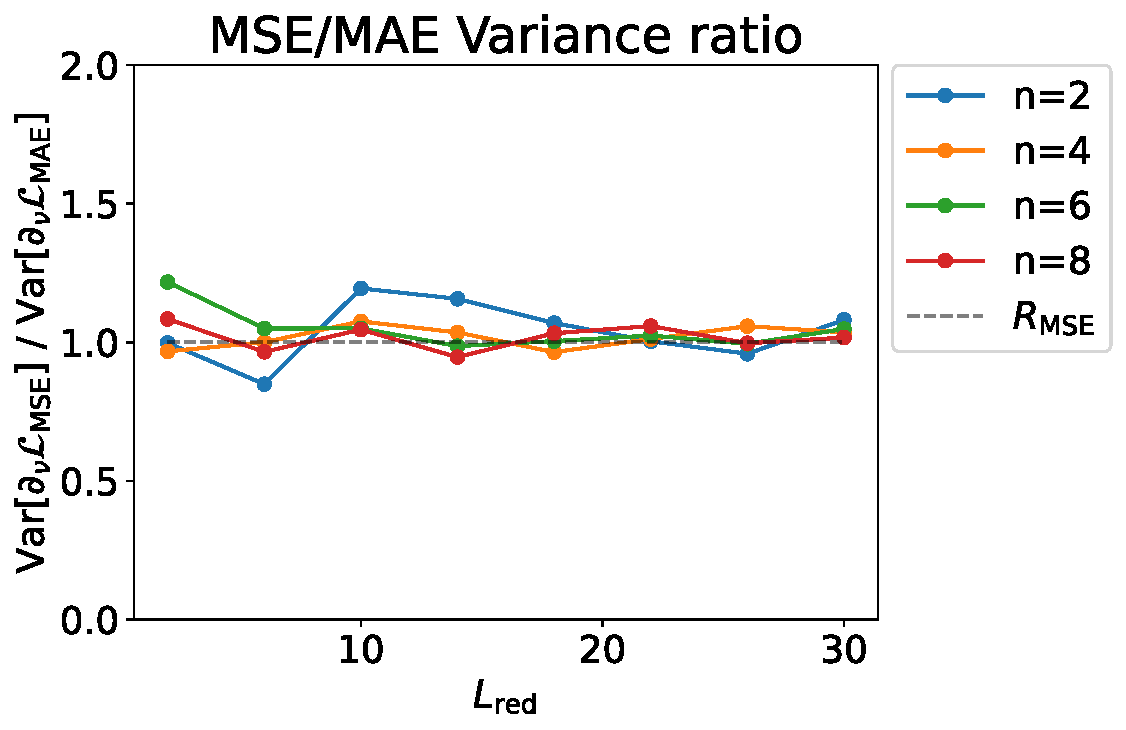
\includegraphics[width=8.5cm]{variance-mse-mae-ratio_encoding3.pdf}
    \end{minipage}
    \begin{minipage}[b]{0.5\columnwidth}
        \centering
        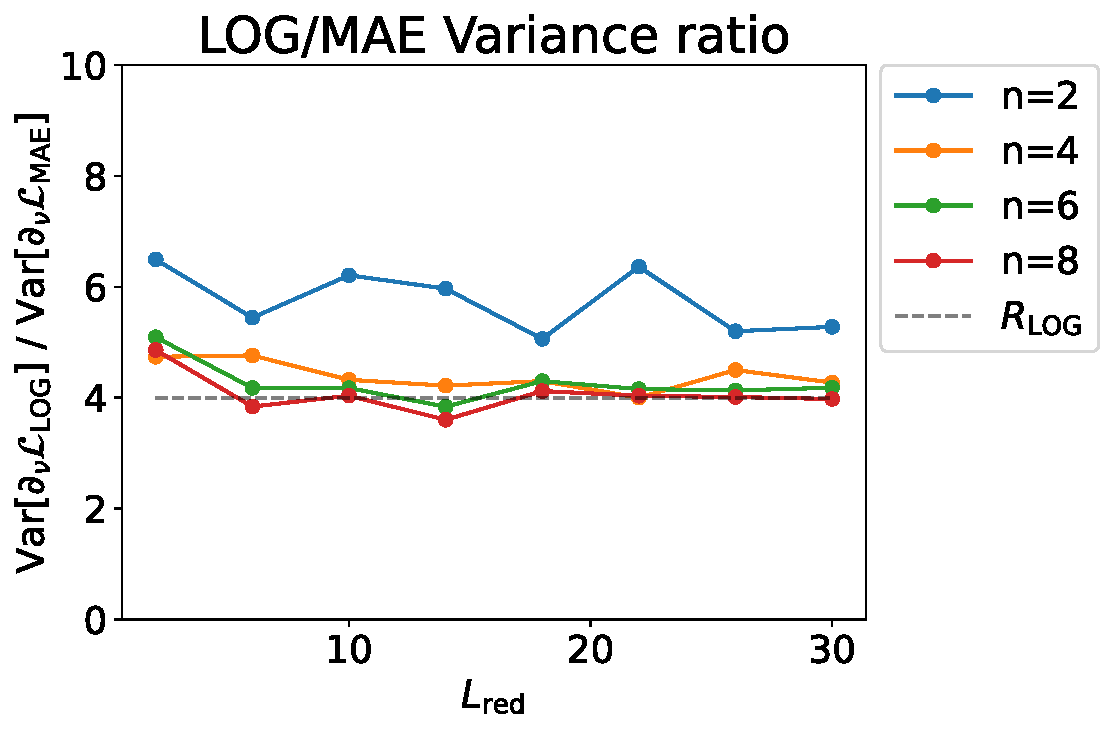
\includegraphics[width=8.5cm]{variance-log-mae-ratio_encoding3.pdf}
    \end{minipage}
    \caption{図~\ref{fig:tpa-alt-circuit}の量子回路を用いて計算したそれぞれのコスト関数の勾配の分散から、絶対誤差の勾配の分散との比を計算した。左は、二乗誤差と絶対誤差の勾配の分散の比、右は、交差エントロピー誤差と絶対誤差の勾配の分散の比をプロットしたものである。破線は、式\eqref{eq:cost-approx-var}で得られた近似比(左: $R_{\mathrm{MSE}}=1$、右: $R_{\mathrm{LOG}}=4$)を表している。}
    \label{fig:qml-var-ratio}
\end{figure}


図~\ref{fig:qml-var-ratio}の左は、二乗誤差と絶対誤差の勾配の分散の比、右は、交差エントロピー誤差と絶対誤差の勾配の分散の比である。破線は、式\eqref{eq:cost-approx-var}の近似比($1$ または $4$)を表している。
両方の数値計算の結果とも、量子ビット数 $n=2$ のときはややばらつきがあるが、各量子ビット数 $n$、学習回路の各層数 $L_{\text{red}}$ において式\eqref{eq:cost-approx-var}の近似比($1$ または $4$)に近い値をとっていることがわかる。
特に、学習回路の層数 $L_{\text{red}}$ が少なく、ユニタリ $2$--デザインを成すには不十分な場合にも、式\eqref{eq:cost-approx-var}の近似比($1$ または $4$)に近い値をとっている。量子ビット数 $n=2$ のときはばらつきがやや大きいのは、量子ビット数が少ないほど $\ell_i(\bs{\th})$ の分散が大きくなり、$\ell_i(\bs{\th}) \sim 1/2$ の近似が成り立たないためであると考えられる。

このことから、数値的にも、二乗誤差と交差エントロピー誤差のコスト関数の勾配の分散は、絶対誤差のコスト関数の勾配の分散と同程度のスケーリングであると考えられる。
したがって、バレンプラトーの解析においては、いずれかひとつについてのみ考えれば、他のコスト関数についても同様の結果が得られると推測される。


以上の議論では $O_{\rmL} = \frac{1}{n} \sum_{j=1}^{n}\dyad{0}_{j} \otimes \bbid_{\bar{j}}$ をオブザーバブルに用いたが、一般的に、Pauli 演算子の線形結合で表されるオブザーバブルを用いても、同様に $\ell_i(\bs{\th})$ の値の集中が示される。
例えば、測定するオブザーバブルを $O = c_{\bs{0}}\bbid + \sum_{\{\bs{i}\}\backslash\bs{0}} c_{\bs{i}}P_{\bs{i}}$ と表す。ただし、$P_{\bs{i}} = \bigotimes_{j=1}^n P_{i_j},\, i_j \in \{0,1,2,3\}$ であり、$P_{i_j}$ は第 $j$ 番目の量子ビットにおける Pauli 演算子、$c_{\bs{i}}$ は実数である。
このとき、$\ell_i(\bs{\th}) = \Tr[V\rho_iV O]$ の平均と分散は次のように計算される。
\begin{align}
    \E_{\calU(d)}[\ell_i(\bs{\th})]   &= c_{\bs{0}}\\
    \Var_{\calU(d)}[\ell_i(\bs{\th})] &= \frac{1}{2^n+1}\sum_{\{\bs{i}\}\backslash\bs{0}} c_{\bs{i}}^2
\end{align}
よって、$\sum_{\{\bs{i}\}\backslash\bs{0}} c_{\bs{i}}^2 \in \order{\poly(n)}$ であれば、チェビシェフの不等式から $\ell_i(\bs{\th})$ は指数関数的に $c_{\bs{0}}$ に集中することがわかる。
したがって、この節における議論は、$O_{\rmL}$ に限らず、一般的なオブザーバブルについても成り立つと考えられる。


\newpage
\newgeometry{top=10truemm,bottom=20truemm,left=20truemm,right=20truemm}
\chapter{結論}

% 目的
近年、機械学習はさまざまな分野で応用され、著しい発展を遂げている。一方で、計算量が膨大であり、計算資源の不足が懸念されている。そこで、量子コンピューターによって機械学習を効率化するための研究が盛んに行われている。本研究は、NISQ 上での実装が可能な変分量子アルゴリズムの文脈において、教師あり量子機械学習の効率化に関する研究を行った。

量子機械学習アルゴリズムの効率化においては、データ入力が重要であることが指摘されている一方で、バレンプラトーという勾配消失問題との関連も指摘されている。バレンプラトーには、量子回路の深さ、オブザーバブルの局所性、ノイズ、データの入力が関係していることが知られている。どれか一つの原因でも存在すると、計算量は量子ビット数に関して指数関数的に増大してしまい、学習がほとんど進まない。しかしながら、これまでのバレンプラトーについては主に学習回路の構造に着目して研究されてきたため、データ入力がバレンプラトーに与える影響は十分には理解されていなかった。そこで、本研究は、量子機械学習に特有のデータ入力がバレンプラトーに与える影響を評価した。
特に、量子機械学習おける識別モデルのバレンプラトーについて、コスト関数の勾配の分散のスケーリングを評価することを目的とした。

% 結果、新規性、考察、貢献
第\ref{chap:upper-bound}章では、量子機械学習おける識別モデルのコスト関数のバレンプラトーについて、学習回路やオブザーバブルの局所性によるバレンプラトーが起きない設定の下で、コスト関数の勾配の分散の上界をデータ入力の観点から導出し、数値的にも検証を行った。
その結果、データ入力後の状態のエンタングルメントや入力回路の表現能力が大きいほど、コスト関数の勾配の分散の上界が小さくなり、バレンプラトーにつながることが明らかになった。
また、量子回路に Depolarizing ノイズを加えた場合に、その上界が更に小さくなることを示した。

第\ref{chap:lower-bound}章では、量子機械学習における識別モデルのコスト関数のバレンプラトーについて、特に、絶対誤差のコスト関数の勾配の分散の下界を、ガウス分布に従う入力データの観点から導出した。これにより、絶対誤差のコスト関数の勾配の分散の下界において、入力データの分散が重要な役割を果たすことを示した。そして、特定の場合において、バレンプラトーを引き起こさないための訓練データの分散に関する十分条件を得た。
また、二乗誤差や交差エントロピー誤差のコスト関数の勾配の分散は、絶対誤差のコスト関数の勾配の分散と同じようにスケールすることを数値的に示した。これにより、量子機械学習におけるバレンプラトーの解析では、どれか1つのコスト関数の勾配の分散を評価すれば十分であると推測される。

% 展望
今後必要となる研究には、次の2点が挙げられる。
まず、本研究では学習回路に単純な構造を仮定したが、より複雑な構造を用いた場合のスケーリングを調べることが望まれる。
また、本研究では量子回路学習モデルのバレンプラトーについてのみ議論したが、より一般的な議論のためには、Data reuploading モデルについても解析が必要である。

しかし、訓練可能性だけが、量子機械学習の性能を決定するわけではない。データ入力のための量子回路の構造には、古典コンピューターによる効率的な計算が難しいこと、汎化性能が高いことなども重要である。将来的に、これらの性能についても評価した上で、量子機械学習のデータ入力を設計することが期待される。
\restoregeometry
\newpage
\chapter*{謝辞}
\addcontentsline{toc}{chapter}{謝辞}

本研究では多くの方にサポートして頂きました。皆様に心より感謝申し上げます。
指導教官である寺師弘二准教授、永野廉人特任助教には、研究の方向性・問題点・計算に関する議論・資料の校正まで何度も付き合って頂き、多くの助言を頂きました。
また、量子コンピューティンググループのミーティングを通して、田中純一教授、澤田龍准教授、飯山悠太郎助教、Wai Yuen Chan特任研究員、加地 俊瑛特任研究員には研究についての質問や指摘、研究発表へのアドバイスを頂きました。
張元豪さん、寺尾萌里乃さん、尾嶋陸斗さん、山崎峻さんにはゼミやミーティングでの議論、日頃の相談に付き合って頂きました。
そして、ICEPP 物理事務室のみなさまには修士過程の生活を送る上で各種サポートをして頂きました。
最後に、日々の生活を支えてくれた家族に心から感謝します。



\newpage
% \bibliographystyle{unsrt}
% \bibliography{ref}
\printbibliography[title=参考文献] % biblatex

\newpage
\appendix
\chapter{第\ref{chap:vqa}章の補足}
\section{機械学習の概要}\label{sec:machine-learning}
機械学習とは、コンピューターに問題を解くためのルールを明示することなく、学習を通して最適なモデルを作る方法である。
機械学習の分野は、教師あり学習、教師なし学習、強化学習の3つの大きなカテゴリに分けられる。

\begin{itemize}
    \item \textbf{教師あり学習}とは、与えられた入力値と出力値のペアの集合(訓練データセット)に基づいて、入力値を出力値にマッピングする関数を学習するタスクである。これにより、関数が未知のデータサンプルの出力値を正しく決定できるようにする。
    \item \textbf{教師なし学習}とは、出力値を持たない入力値のみのデータセットからの推論を行うために使用される機械学習のタスクである。最も一般的な教師なし学習の方法はクラスター分析であり、これはデータ内の隠れたパターンやグループを見つけるための探索的データ分析に使用される。
    \item \textbf{強化学習}とは、ソフトウェア上のエージェントが環境との相互作用を通じて学習する機械学習のタスクである。強化学習は、教師あり学習とは異なり、正しい出力が何であるかを明示的に教えられない。代わりに、エージェントは、試行錯誤のプロセスを通じて報酬または罰則を受け取り、その結果、最適な行動を決定するための行動戦略を学習する。
\end{itemize}


\subsection{教師あり学習のモデル}
教師あり学習の問題を記述するために、入力の集合 $X$ と出力の集合 $Y$ を定義する。また、仮説の集合 $H$ を定義する。$H$ は $X$ から $Y$ へのすべての関数の集合の部分集合である。$H$ を仮説空間と呼ぶ。また、$S = \{(x,y)|x\in X, y\in Y\}$ とし、訓練サンプルの集合 $D$ は $S$ の部分集合であるとする。同様に、テストサンプルの集合 $T$ も $S$ の部分集合であるとする。ただし、$D$ と $T$ は共通の要素を持たないとする。
教師あり学習の目的は、$D$ に基づいて $H$ の中の最適な仮説 $h$ を見つけることである。最適な仮説 $h$ は、$T$ に基づいてテストされる。$h$ が $T$ でうまく機能する場合、$h$ は未知の入力 $x$ に対してもうまく機能すると予想される。

損失関数 $L$ は、仮説 $h$ と訓練サンプル $(x, y)$ を入力として受け取り、$h$ が $x$ に対して $y$ を正しく予測しなかった場合のペナルティを計算する関数である。
損失関数の単純な例は、次のように定義される二乗誤差である。
\begin{align}
    L(h, (x, y)) = (h(x) - y)^2.
\end{align}

教師あり学習は、訓練データセット $D$ と損失関数 $L$ によって定義される経験損失 $\E[L(h, (x, y))]$ を最小化する仮説 $h$ を見つける。
\begin{align}
    \E[L(h, (x, y))] = \sum_{(x, y) \in D} L(h, (x, y)).
\end{align}

\subsection{教師なし学習のモデル}
教師なし学習では、空間 $X$ のベクトルとして表されるデータサンプルの集合 $D$ が与えられる。教師なし学習の目的は、データの構造を発見することである。構造は通常、クラスターの集合によって記述される。各クラスターは $D$ の部分集合であり、すべてのクラスターの和集合は $D$ である。教師なし学習の目的は、$D$ の良い分割であるクラスターの集合 $C$ を見つけることである。良い分割とは、同じクラスター内の任意の2点間の距離が小さいことと、異なるクラスター内の任意の2点間の距離が大きいことを意味する。
コスト関数 $J$ は、クラスターの集合 $C$ を入力として受け取り、クラスターの集合 $C$ が $D$ の良い分割である場合に小さい値を返す関数である。
\begin{align}
    J(C) = \sum_{C_i \in C} \sum_{x, y \in C_i} \norm{x - y}^2.
\end{align}

\subsection{強化学習のモデル}
強化学習では、アクションの集合 $A$、状態の集合 $S$、および報酬関数 $R$ が与えられる。報酬関数は、エージェントが特定の状態 $s \in S$ にいて特定のアクション $a \in A$ を取った場合の報酬を計算する。
強化学習の目的は、状態を入力として受け取り、アクションを返す関数である方策 $\pi$ のなかで、期待される総報酬を最大化する方策を見つけることである。
具体的には、状態価値関数や行動価値関数を用いて、方策を最適化する。

状態価値関数 $V^{\pi}(s)$ は、最初に状態 $s$ にあり、その後方策 $\pi$ に従って行動を選択することを繰り返した場合の期待される総報酬である。
\begin{align}
    V^{\pi}(s) = \E_{\pi}\qty[\sum_{t=0}^{\infty} \gamma^t R(s_t, a_t) | s_0 = s].
\end{align}
ここで、$\gamma \in [0, 1]$ は割引率である。

行動価値関数 $Q^{\pi}(s, a)$ は、最初に状態 $s$ にあり、行動 $a$ を選択し、その後方策 $\pi$ に従って行動を選択することを繰り返した場合の期待される総報酬である。
\begin{align}
    Q^{\pi}(s, a) = \E_{\pi}\qty[\sum_{t=0}^{\infty} \gamma^t R(s_t, a_t) | s_0 = s, a_0 = a].
\end{align}
これらの価値関数に対して、価値反復法や Q 学習などのアルゴリズムを用いて、最適な方策を見つける。



% \section{ニューラルネットワーク}
% ニューラルネットワークとは、神経細胞(ニューロン)のネットワークを意味するが、最近では、機械学習における人工的なノードからなるネットワークを意味することも多い。
% 後者のニューラルネットワークは、入力層、中間層、出力層から構成される。中間層は、隠れ層とも呼ばれる。ニューラルネットワークは、入力層から出力層への情報の流れを表す有向グラフで表現される。各層は、ノードの集合で表現される。各ノードは、前の層のノードからの入力を受け取り、出力を次の層のノードに送信する。各ノードは、入力に対して重み付けされた値を計算し、活性化関数を適用する。活性化関数は、ノードの出力を計算するために使用される非線形関数である。ニューラルネットワークの学習は、訓練データセットを使用して、ニューラルネットワークの重みを調整することである。ニューラルネットワークの重みは、訓練データセットに基づいて、ニューラルネットワークの出力が訓練データセットの出力に近づくように調整される。ニューラルネットワークの学習は、誤差逆伝播法と呼ばれるアルゴリズムによって実行される。誤差逆伝播法は、ニューラルネットワークの出力の誤差を計算し、誤差を最小化するようにニューラルネットワークの重みを調整する。


% 神経細胞(ニューロン)のネットワークを意味するが、最近では、コンピューター上での人工的なノードからなるネットワークを意味することが多い。よって、ニューラルネットワークは、生物学的ニューロンからなる生物学的ニューラルネットワークであるか、人工知能(AI)の問題を解決するための人工ニューラルネットワークである。生物学的ニューロンの接続強さは重みと呼ばれる数値としてモデル化される。正の重みは興奮性の接続を反映し、負の値は抑制性の接続を意味する。各ニューロンの出力は、他のニューロンに入力として渡される。これらのニューロンにはしきい値があるため、入力がそのしきい値を超えた場合にのみ考慮される。入力は、前の層の他のニューロンまたはノードの出力の加重和である。加重和は、非線形関数(活性化関数と呼ばれる)を介して変換される。そのニューロンの出力は、他のニューロンに入力として渡される。このプロセスは、ネットワーク内の各ニューロンに対して繰り返される。ネットワークの出力層は出力ベクトルを生成する。このベクトルの各要素は、入力が特定のクラスに属する確率に対応する。確率が最も高い出力は、入力のクラスラベルである。



% \section{カーネル法}
% \begin{screen}
%     \begin{theorem}
%         Representer theorem
        
%         Let $K$ be a positive definite kernel on $\calX$, and let $L$ be a strictly increasing function from $\bbR$ to $\bbR$. Let $H_k$ be the reproducing kernel Hilbert space associated with $K$. Then, for any training set $T = \{(x_1, y_1), \ldots, (x_n, y_n)\}$, the minimizer $f^\ast(\cdot)$ of the regularized empirical risk minimization problem
%         \begin{equation}
%             \min_{f \in H_k} \qty{ \frac{1}{n} \sum_{i=1}^n L(f(x_i), y_i) + \lambda \norm{f}_{H_k}^2}
%         \end{equation}
%         can be written as
%         \begin{equation}
%             f^\ast(\cdot) = \sum_{i=1}^n \alpha_i K(\cdot, x_i)
%         \end{equation}
%         for some $\bs{\alpha} = (\alpha_1, \ldots, \alpha_n) \in \bbR^n$.
%     \end{theorem}
% \end{screen}



\newpage
\section{ユニタリ $2$--デザインにおけるバレンプラトーの定理と証明}\label{sec:bp-proof}
先行研究\cite{mcclean2018barren}はバレンプラトーという現象を最初に示した。ここでは、その論文の結果と証明を紹介する。
ユニタリ $2$--デザインの定義については、\ref{sec:unitary-t-design}~節を参照されたい。
\begin{screen}
    \begin{theorem}\label{thm:bp}
        量子回路 $V(\bs{\th})$ は $n$ 個の量子ビットからなり、2つの部分 $V(\bs{\th}) = V_+V_-$, $V_+ := \prod_{l=k+1}^L U_l(\th_l)W_l$, $V_- := \prod_{l=1}^{k} U_l(\th_l)W_l$ に分解できるとする。$V_+,\, V_-$ の少なくとも一方がユニタリ $2$--デザインであるとき、コスト関数 $C(\bs{\th}) = \Tr[V(\bs{\th})\rho V\dg(\bs{\th})O]$ はバレンプラトーとなる~\cite{mcclean2018barren}。
        \begin{align}
            \Var_{V(\bs{\th})}\qty[\pdv{C(\bs{\th})}{\th_k}]
            =
            \begin{cases}
                -\frac{1}{4}\frac{\ev{\Tr[P_-^2]}_{V_-}}{d^2-1}\qty(\Tr[O^2] - \frac{\Tr[O]^2}{d}) & \text{if $V_+$ is $2$--design}\\
                -\frac{1}{4}\frac{\ev{\Tr[P_+^2]}_{V_+}}{d^2-1}\qty(\Tr[\rho^2] - \frac1d) & \text{if $V_-$ is $2$--design}\\
                \frac{d^2}{2(d^2-1)^2}\qty(\Tr[O^2] - \frac{\Tr[O]^2}{d})\qty(\Tr[\rho^2] - \frac1d) & \text{if $V_+,V_-$ are $2$--design}
            \end{cases}
        \end{align}
        ここで、$U_k(\th_k) = \exp(-\frac{i}{2}\th_k P_k),\,(P_k^2 = I,\, \Tr[P_k] = 0)$, $P_+ := [P_k, V_+\dg OV_+]$, $P_- := [P_k, V_-\rho V_-\dg]$ とした。
    \end{theorem}
\end{screen}

量子回路がユニタリ $t$--デザインならば、ユニタリ $(t-1)$--デザインでもあるので、ユニタリ $t \geq 2$ --デザインならば、バレンプラトーが起きる。

% \begin{align}
%     \Delta(A) &:= D_{\HS}\qty(A, \Tr[A]\frac{\bbid}{d})\\
%     \Var_{V(\bs{\th})}\qty[\pd_k C(\bs{\th})]
%     &=
%     \frac{2d^2}{(d^2-1)}\Delta(H)\Delta(\rho)\Delta(P_k)
% \end{align}

\begin{proof}\label{proof:bp}
    $U_k(\th_k) = \exp(-\frac{i}{2}\th_k P_k)$ と表され、$P_k \in \{X,Y,Z\}$ とする。このとき、$\pd_k V(\bs{\th}) = -\frac{i}{2}V_+P_kV_-$ であるから、
    \begin{align}
        \pd_k C(\bs{\th}) := \frac{\pd C(\bs{\th})}{\pd \theta_k}
        &= \frac{i}{2}\qty(\Tr[V_+V_-\rho V_-\dg P_kV_+\dg O] - \Tr[V_+P_kV_-\rho V_-\dg V_+\dg O])\\
        &= -\frac{i}{2}\Tr[ V_+\dg OV_+\, [P_k, V_-\rho V_-\dg]]\\
        &=\;\;\;\frac{i}{2}\Tr[V_-\rho V_-\dg\, [P_k, V_+\dg OV_+]]
    \end{align}
    最後の等式では $\Tr[A[B,C]] = -\Tr[C[B,A]]$ であることを用いた。
    
    まず、勾配の平均が $0$ になることを示す。$V_+$ がユニタリ $2$--デザインであるとすると、$V_+$ はユニタリ $1$--デザインでもあるから、
    \begin{align}
        \E_{V_+}\qty[\pd_k C(\bs{\th})]
        &= -\frac{i}{2}\int_{\calU(d)} d\mu_{\Haar}(V_+) \Tr[ V_+\dg OV_+\, [P_k, V_-\rho V_-\dg]]\\
        &= -\frac{i}{2}\Tr[\qty(\int_{\calU(d)} d\mu_{\Haar}(V_+) V_+\dg OV_+)\, [P_k, V_-\rho V_-\dg]]\\
        &= -\frac{i}{2}\Tr[\frac{\Tr[\rho]\bbid}{d} \times [P_k, V_-\rho V_-\dg]]\quad \because \eqref{eq:haar-int-3}\\
        &= 0 
    \end{align}
    
    同様に、$V_-$ がユニタリ $2$--デザインであるとすると、$V_-$ はユニタリ $1$--デザインでもあるから、
    \begin{align}
        \E_{V_-}\qty[\pd_k C(\bs{\th})]
        &= \frac{i}{2}\int_{\calU(d)} d\mu_{\Haar}(V_-) \Tr[V_-\rho V_-\dg\, [P_k, V_+\dg OV_+]]\\
        &= \frac{i}{2}\Tr[\qty(\int_{\calU(d)} d\mu_{\Haar}(V_-) V_-\rho V_-\dg)\, [P_k, V_+\dg OV_+]]\\
        &= \frac{i}{2}\Tr[\frac{\Tr[\rho]\bbid}{d} \times [P_k, V_+\dg OV_+]]\quad \because \eqref{eq:haar-int-3}\\
        &= 0
    \end{align}
    故に、どちらの場合も $\E_{V(\bs{\th})}[\pd_k C(\bs{\th})] = 0$ である。
    
    次に、勾配の分散が量子ビット数に関して指数関数的に小さくなることを示す。
    $V_-$ がユニタリ $2$--デザインであるとすると、$P_+ := [P_k, V_+\dg OV_+]$ として、
    \begin{align}
        \Var_{V_+}\qty[\pd_k C(\bs{\th})]
        &= -\frac{1}{4}\int_{\calU(d)} d\mu_{\Haar}(V_-) \Tr[V_-\rho V_-\dg\, P_+]\Tr[V_-\rho V_-\dg\, P_+]
    \end{align}
    公式~\eqref{eq:haar-int-5}において、$A = C = \rho$, $B = D = P_+$ とすると、
    \begin{align}
        \Var_{V_-}\qty[\pd_k C(\bs{\th})]
        &= -\frac{1}{4}\Bigg(
        \frac{1}{d^2-1}
        (\Tr[\rho]\Tr[P_+]\Tr[\rho]\Tr[P_+] + \Tr[\rho^2]\Tr[P_+^2]) \nonumber\\
        &\quad\;- \frac{1}{d(d^2-1)}
        (\Tr[\rho^2]\Tr[P_+]\Tr[P_+] + \Tr[\rho]\Tr[\rho]\Tr[P_+^2])\Bigg)\\
        &= -\frac{1}{4}\frac{\Tr[P_+^2]}{d^2-1}\qty(\Tr[\rho^2] - \frac{1}{d}) \quad (\because \Tr[P_+] = 0,\, \Tr[\rho] = 1)
    \end{align}
    
    $V_+$ がユニタリ $2$--デザインとすると、$P_- := [P_k, V_-\rho V_-\dg]$ として、
    \begin{align}
        \Var_{V_+}\qty[\pd_k C(\bs{\th})]
        &= -\frac{1}{4}\int_{\calU(d)} d\mu_{\Haar}(V_+) \Tr[V_+\dg OV_+\, P_-]\Tr[V_+\dg OV_+\, P_-]
    \end{align}
    公式~\eqref{eq:haar-int-5}を用いて同様に計算すると、
    \begin{align}
        \Var_{V_+}\qty[\pd_k C(\bs{\th})]
        &= -\frac{1}{4}\frac{\Tr[P_-^2]}{d^2-1}\qty(\Tr[O^2] - \frac{\Tr[O]^2}{d}) \quad (\because \Tr[P_-] = 0)
    \end{align}
    
    最後に $V_+, V_-$ の両方がユニタリ $2$--デザインであるとする。$\Var_{V_-}\qty[\pd_k C(\bs{\th})]$ を計算したので、あとは、$\Tr[P_+^2]$ を $V_+$ で積分すればよい。
    \begin{align}
        \int_{\calU(d)} d\mu_{\Haar}(V_+) \Tr[P_+^2]
        &= \int_{\calU(d)} d\mu_{\Haar}(V_+) \Tr[[P_k, V_+\dg OV_+]^2]\\
        &= \int_{\calU(d)} d\mu_{\Haar}(V_+)
        \Tr\Big[P_k V_+\dg OV_+ P_k V_+\dg OV_+ + V_+\dg OV_+ P_k V_+\dg OV_+ P_k\nonumber\\
        &\qquad\qquad\qquad\qquad\quad - P_k V_+\dg OV_+ V_+\dg OV_+ P_k -  V_+\dg OV_+ P_k P_k V_+\dg OV_+\Big]\\
        &= \int_{\calU(d)} d\mu_{\Haar}(V_+)\,
        2\times\qty(\Tr[P_k V_+\dg OV_+ P_k V_+\dg OV_+]- \Tr[O^2])\\
        &= \int_{\calU(d)} d\mu_{\Haar}(V_+)\,
        2\times\qty(\Tr[OV_+ P_k V_+\dg OV_+P_kV_+\dg]- \Tr[O^2])
    \end{align}
    最後から2番目の等式では、$P_k^2 = \bbid,\,V_+V_+\dg = \bbid$ を用いた。
    公式~\eqref{eq:haar-int-4}において、$A = C = O$, $B = D = P_k$, $E = \bbid$ とし、全体のトレースを取ると、
    \begin{align}
        \int_{\calU(d)} d\mu_{\Haar}(V_+) \Tr[P_k V_+\dg OV_+ P_k V_+\dg OV_+]
        &= \frac{1}{d^2-1}(\Tr[P_k]\Tr[P_k]\Tr[O^2] + \Tr[P_k^2]\Tr[O]\Tr[O]) \nonumber\\
        &- \frac{1}{d(d^2-1)}(\Tr[P_k^2]\Tr[O^2] + \Tr[P_k]\Tr[O]\Tr[P_k]\Tr[O])\\
        &= \frac{1}{d^2-1}\qty(d\Tr[O]^2 - \Tr[O^2])
    \end{align}
    最後の等式では、$\Tr[P_k] = 0,\,\Tr[P_k^2] = \Tr[\bbid] = d$ を用いた。
    よって、
    \begin{align}
        \int_{\calU(d)} d\mu_{\Haar}(V_+) \Tr[P_+^2]
        &= 2\times \qty(\frac{1}{d^2-1}\qty(d\Tr[O]^2 - \Tr[O^2]) - \Tr[O^2])\\
        &= - \frac{2d^2}{d^2-1}\qty(\Tr[O^2] - \frac{\Tr[O]^2}{d})
    \end{align}
    
    したがって、
    \begin{align}
        \Var_{V(\bs{\th})}\qty[\pd_k C(\bs{\th})]
        &= \frac{d^2}{2(d^2-1)^2}\qty(\Tr[O^2] - \frac{\Tr[O]^2}{d})\qty(\Tr[\rho^2] - \frac{1}{d})
    \end{align}
\end{proof}
% \end{comment}
\newgeometry{top=15truemm,bottom=15truemm,left=20truemm,right=20truemm}
\chapter{第\ref{chap:upper-bound}章の補足}

% \section{補題\ref{lem:variance-inequality}の証明}\label{sec:prf-lemma-variance-inequality}
% \begin{screen}
    % \begin{lemma}
    %     分散についての以下の不等式が成り立つ。
    %     \begin{align}
    %         \Var\Big[\sum_i X_i\Big] &\leq N\sum_i\Var[X_i],\\
    %         \Var[XY] &\leq 2\Var[X]\abs{Y^2}_{\max} + 2(\E[X])^2\Var[Y]\,.
    %     \end{align}
    % \end{lemma}
% \end{screen}

% \begin{proof}
%     We have
%     $$
%     \begin{aligned}
%     \operatorname{Var}[X+Y] & =\operatorname{Var}[X]+\operatorname{Var}[Y]+2 \operatorname{Cov}[X, Y] \\
%     & \leqslant \operatorname{Var}[X]+\operatorname{Var}[Y]+2 \sqrt{\operatorname{Var}[X] \operatorname{Var}[Y]} \\
%     & \leqslant \operatorname{Var}[X]+\operatorname{Var}[Y]+\sqrt{\operatorname{Var}[X] \operatorname{Var}[X]}+\sqrt{\operatorname{Var}[Y] \operatorname{Var}[Y]} \\
%     & =2 \operatorname{Var}[X]+2 \operatorname{Var}[Y]
%     \end{aligned}
%     $$
%     32
%     where in the first inequality we have used Cauchy-Schwarz, and the second inequality comes from the rearrangement inequality. Now consider
%     $$
%     \begin{aligned}
%     \operatorname{Var}[X Y] & =\operatorname{Var}[(X-\mathbb{E}[X]) Y+\mathbb{E}[X] Y] \\
%     & \leqslant 2 \operatorname{Var}[(X-\mathbb{E}[X]) Y]+2 \operatorname{Var}[\mathbb{E}[X] Y] \\
%     & \leqslant 2 \mathbb{E}\left[(X-\mathbb{E}[X])^2 Y^2\right]+2(\mathbb{E}[X])^2 \operatorname{Var}[Y] \\
%     & \leqslant 2 \mathbb{E}\left[(X-\mathbb{E}[X])^2\right]\left|Y^2\right|_{\text {max }}+2(\mathbb{E}[X])^2 \operatorname{Var}[Y] \\
%     & =2 \operatorname{Var}[X]\left|Y^2\right|_{\text {max }}+2(\mathbb{E}[X])^2 \operatorname{Var}[Y]
%     \end{aligned}
%     $$
%     where in the first inequality we have used Eq. (G5), in the second inequality we have used the definition of the variance, and in the third inequality we have simply taken the maximum value for $Y^2$.
% \end{proof}

\section{ローカルユニタリ $2$--デザイン: ALT の計算例}\label{sec:alt-calculation}
ここでは、ローカルユニタリ $2$--デザインの仮定の下での $\int_{U\in\bbU} dU D_{\HS} (\rho^{(h)} , \bbid/2^s)$ の計算について、量子ビット数が $6$、層数が $3$、$s = 1$ の場合の例を用いて説明する。
$D_{\HS} (\rho^{(h)} , \bbid/2^s) = \operatorname{Tr}[(\rho^{(h)})^2] - 1/2^s$ であるから、$\int_{U\in\bbU} dU \operatorname{Tr}[(\rho^{(h)})^2]$ を計算すれば良い。$\operatorname{Tr}[(\rho^{(h)})^2]$ をテンソルネットワークで表現すると、図~\ref{fig:tn-alt-int-1} の一番上のネットワークのようになる。これを、各ゲートブロックがユニタリ $2$--デザインを成すとして積分する。
以降の図では、$UU\dg = \bbid$ となって消える部分を灰色で表現している。図の最初の等号では、灰色の部分を消した。
2つ目の等号は、$U_1$ のみを、図~\ref{fig:haar-int-4}を用いて積分した。
\begin{figure}[H]
    \centering
    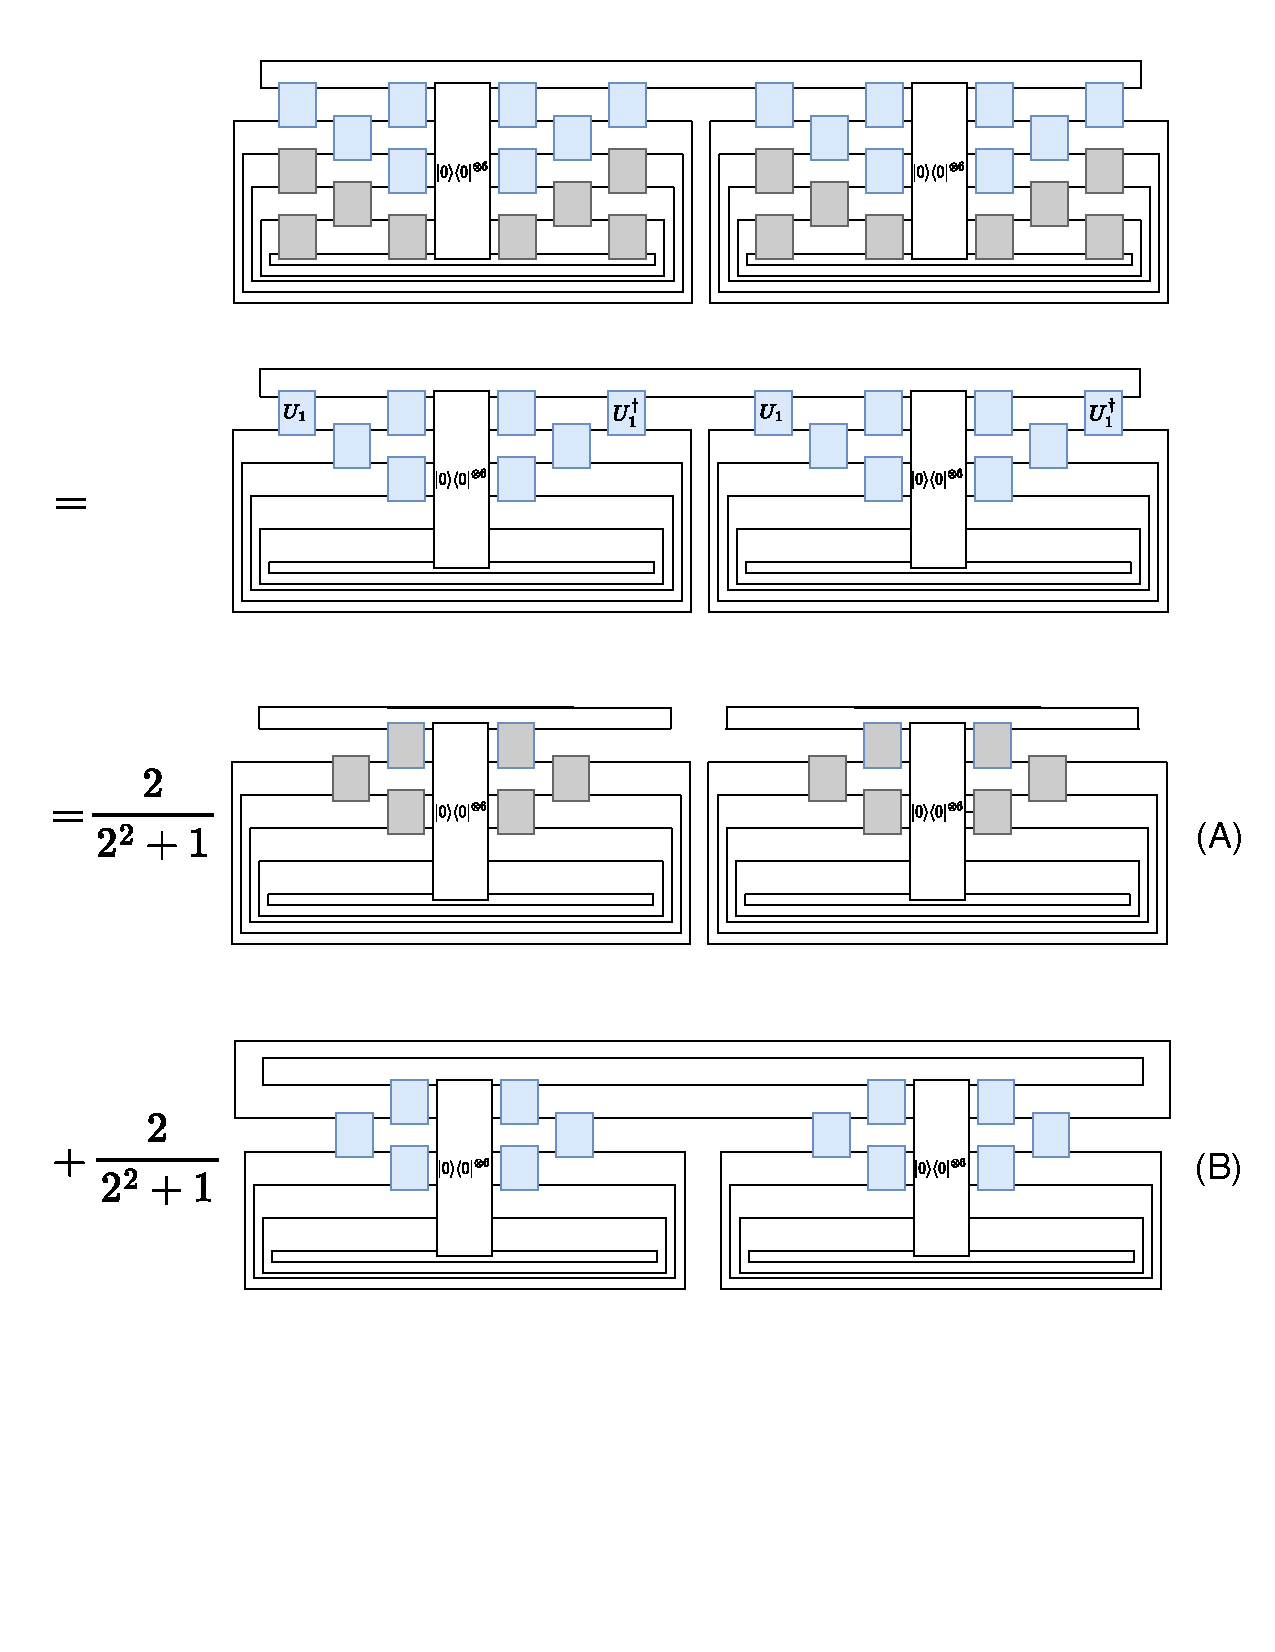
\includegraphics[width=15cm]{int-ALT-Page-1.drawio.pdf}
    \vspace{-20pt}
    \caption{量子ビット数が $6$、層数が $3$、$s = 1$ の ALT において、$U_1$ を図~\ref{fig:haar-int-4}を用いて積分}
    \label{fig:tn-alt-int-1}
\end{figure}

これにより出てきた2つの項(A)と(B)について:まず、項(A)は $(\operatorname{Tr}[U\dyad{0}\otn{6}U\dg])^2 = 1$ である。次に項(B)については、図~\ref{fig:tn-alt-int-2}の一番上のネットワークのゲートブロック $U_2$ を積分すると項(C), (D)に分解される。
\begin{figure}[H]
    \centering
    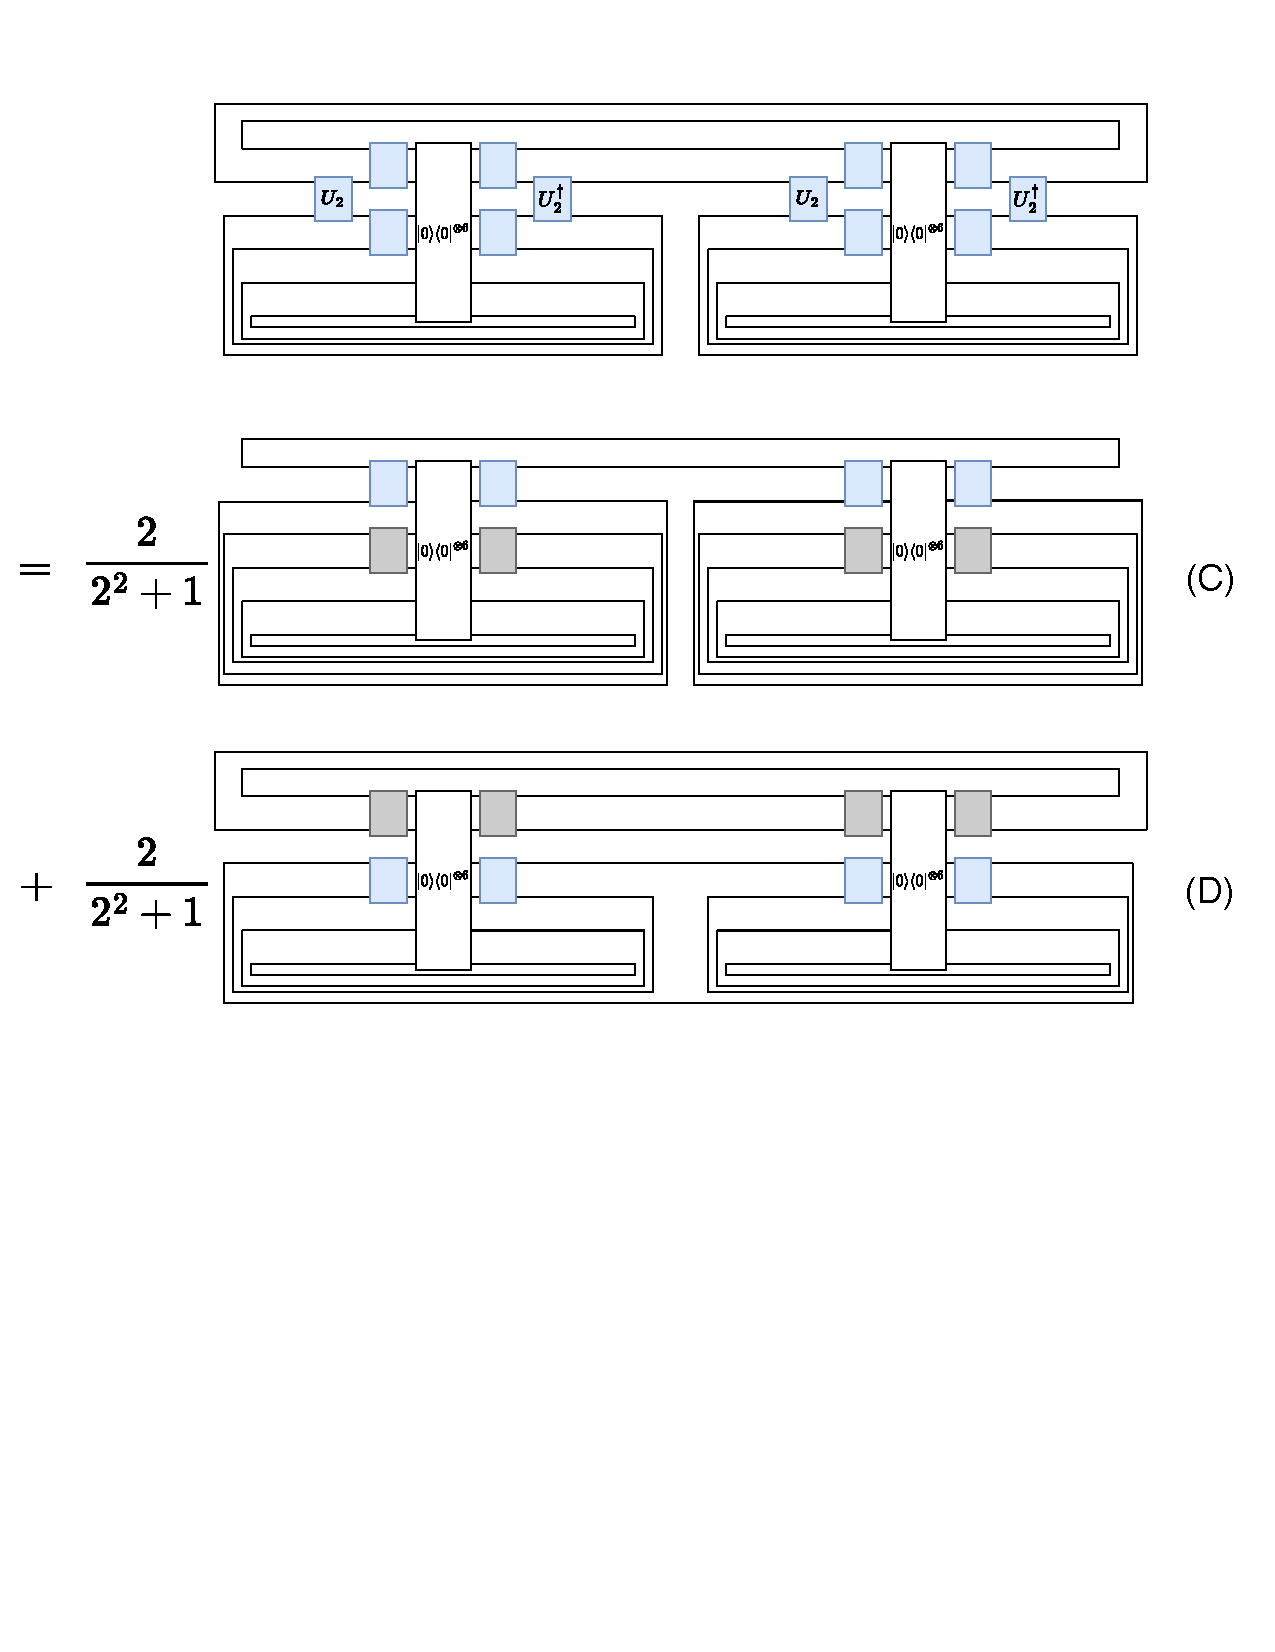
\includegraphics[width=15cm]{int-ALT-Page-2.drawio.pdf}
    \vspace{-20pt}
    \caption{項(B)について、$U_2$ を図~\ref{fig:haar-int-4}を用いて積分した計算の例。}
    \label{fig:tn-alt-int-2}
\end{figure}

以上の計算で出てきた、項(C), (D)は、$UU\dg = \bbid,\,\operatorname{Tr}[\dyad{0}] = 1$ であることを用いると、次の図のようになる。
\begin{figure}[H]
    \centering
    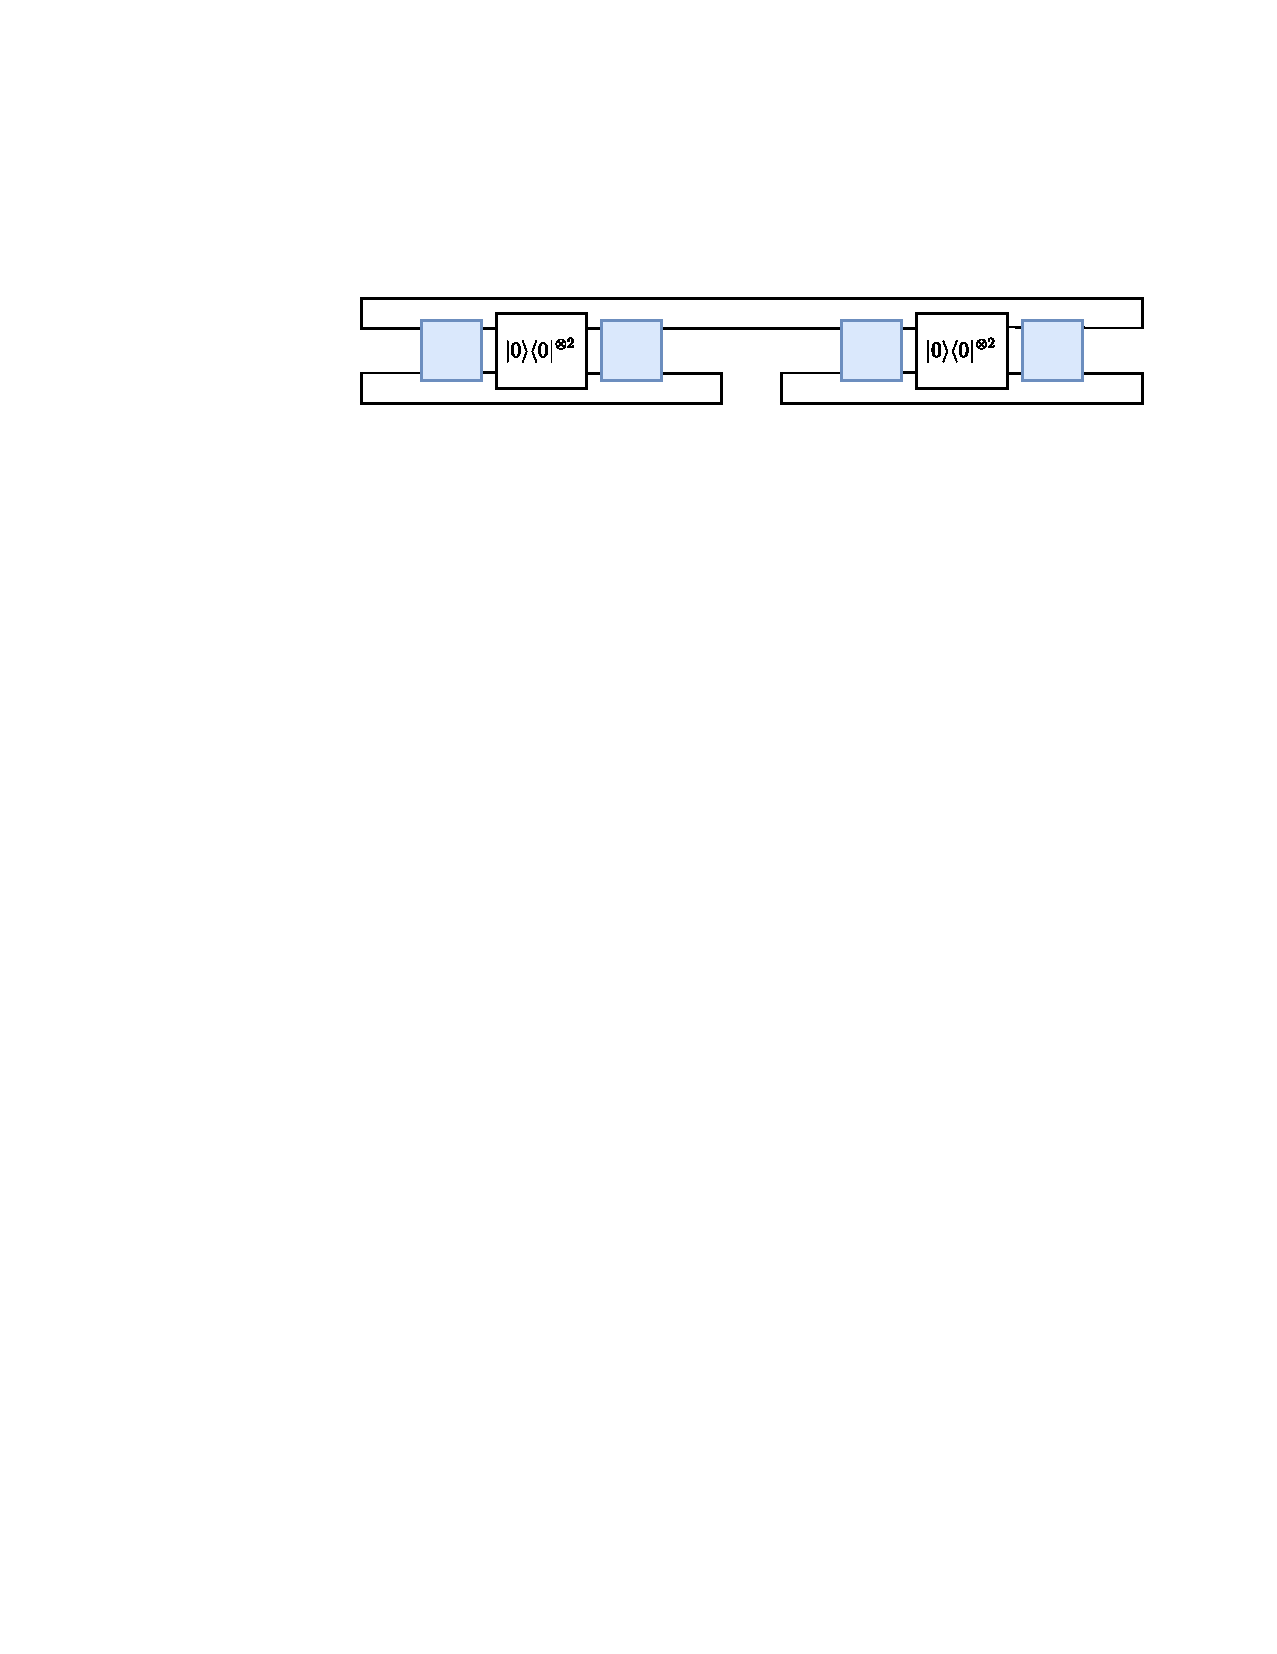
\includegraphics[width=13cm]{int-ALT-Page-3.pdf}
    \label{fig:tn-alt-int-3}
\end{figure}
この計算は、定理\ref{thm:dhs-haar-int}において、$n = 2,\,s = 1$ とした場合に相当するので、$\frac{2^{2-1} + 2^1}{2^2 + 1} = \frac45$ となる。
したがって、$\int_{U\in\bbU} dU \operatorname{Tr}[(\rho^{(h)})^2]$ は、
\begin{align*}
    \int_{U\in\bbU} dU \operatorname{Tr}[(\rho^{(h)})^2]
    &= \frac{2}{2^2 + 1}\times\text{(A)} + \frac{2}{2^2 + 1}\times\text{(B)}\\
    &= \frac{2}{2^2 + 1}\times\text{(A)} + \frac{2}{2^2 + 1}\qty[\frac{2}{2^2 + 1}\times\text{(C)} + \frac{2}{2^2 + 1}\times\text{(D)}]\\
    &= \frac{2}{2^2 + 1}\times1 + \frac{2}{2^2 + 1}\qty[\frac{2}{2^2 + 1}\times\frac45 + \frac{2}{2^2 + 1}\times\frac45]\\
    &= \frac{82}{125}
\end{align*}
\restoregeometry

$\int_{U\in\bbU} dU \operatorname{Tr}[(\rho^{(h)})^2]$ を各層、各量子ビットについて、同様の計算を行った結果が、表~\ref{tab:alt-tr-int} である。これから $\int_{U\in\bbU} dU D_{\HS} (\rho^{(h)} , \bbid/2^{s=1}) = \int_{U\in\bbU} dU \operatorname{Tr}[(\rho^{(h)})^2] - 1/2^{s=1}$ を計算してプロットしたものが図~\ref{fig:hsd-alt-analytical} である。

\begin{table}[H]
    \centering
    \caption{各量子ビット $n$、各層 $L$、$s = 1$ の ALT における $\int_{U\in\bbU} dU \operatorname{Tr}[(\rho^{(h)})^2]$ の計算結果。}
    \label{tab:alt-tr-int}
    \begin{tabular}{c|cccccccc}
        \hline
        $n \backslash L$ & $2$ & $4$ & $6$ & $8$ & $10$ & $12$& $14$ & $16$\\
        \hline
        $2$ & $\frac45$ & $\frac45$ &  $\frac45$ &  $\frac45$ &  $\frac45$ & $\frac45$ & $\frac45$ & $\frac45$ \\
        $4$ & $\frac{18}{5^2}$ & $\frac{394}{5^4}$ & $\frac{9402}{5^6}$ & $\frac{231466}{5^8}$ & $\frac{5757978}{5^{10}}$ & $\frac{143720074}{5^{12}}$ & $\frac{3591166842}{5^{14}}$ & $\frac{89764490986}{5^{16}}$\\
        $6$ &$\frac{18}{5^2}$ & $\frac{386}{5^4}$ & $\frac{8882}{5^6}$ & $\frac{212834}{5^8}$ & $\frac{5210258}{5^{10}}$ & $\frac{128929346}{5^{12}}$ & $\frac{3207308402}{5^{14}}$ & $\frac{79991607074}{5^{16}}$\\
        $8$ & $\frac{18}{5^2}$ & $\frac{386}{5^4}$ & $\frac{8850}{5^6}$ & $\frac{210498}{5^8}$ & $\frac{5116018}{5^{10}}$ & $\frac{125901602}{5^{12}}$ & $\frac{3120244306}{5^{14}}$ & $\frac{77633338882}{5^{16}}$\\
        \hline
    \end{tabular}
\end{table}

\chapter{第\ref{chap:lower-bound}章の補足}



\section{定理\ref{cor:covariance}の略証}\label{sec:prf-covariance}
\begin{screen}
\begin{corollary}
    (論文~\cite{cerezo2021cost}の Supplementary Note 5, B の拡張された結果)
    図~\ref{fig:circuit-setting}の回路に対して、次の式が成り立つ。
    \begin{align}
        \E_{V(\bs{\th})}[\pd_\nu\ell_i\,\cdot\,\pd_\nu\ell_j] = \frac{2^{2s-1}\Delta\Omega}{\qty(2^{2s}-1)^2}\qty(\Tr\qty[\rho_i^{(h)}\rho_j^{(h)}]-\frac{1}{2^s})
    \end{align}
    ただし、$\Delta\Omega = \operatorname{Tr}[(\widehat{O}_\rmL^{(h)})^2] - \frac{1}{2^s}(\operatorname{Tr}[\widehat{O}_\rmL^{(h)}])^2$
\end{corollary}
\end{screen}

\begin{proof}
    まず、論文~\cite{cerezo2021cost}の「Supplementary Note 4: Variance of the cost function partial derivative」の結果を拡張する。具体的には、$\rho \rightarrow \rho_i$ というように入力状態にインデックスを付け、勾配の共分散を計算する。
    \begin{screen}
        \begin{theorem}\label{thm:supplementary-4}
            (論文~\cite{cerezo2021cost}の「Supplementary Note 4: Variance of the cost function partial derivative」の拡張された結果)
            \begin{align}
                \E_{V(\bs{\th})}[\pd_\nu\ell_i\,\cdot\,\pd_\nu\ell_j]
                &= \frac{2^{m-1} \Tr\left[\sigma_\nu^2\right]}{\left(2^{2 m}-1\right)^2} 
                \sum_{\substack{\vb*{pq}\\\vb*{p^{\prime} q^{\prime}}}}
                \expval{\Delta \Omega_{i;\vb*{pq}}^{j;\vb*{p^{\prime} q^{\prime}}}}_{V_\rmR}
                \expval{\Delta\Psi_{i;\vb*{pq}}^{j;\vb*{p^{\prime} q^{\prime}}}}_{V_{\rmL}},\\
                \Delta\Omega_{\vb*{pq}}^{\vb*{p^{\prime} q^{\prime}}}
                &:= \Tr\qty[\Omega_{\vb*{qp}} \Omega_{\vb*{p^{\prime} q^{\prime}}}]-\frac{\Tr\qty[\Omega_{\vb*{qp}}] \Tr\qty[\Omega_{\vb*{p^{\prime} q^{\prime}}}]}{2^m}, \nonumber\\
                \Delta \Psi_{i;\vb*{pq}}^{j;\vb*{p^{\prime} q^{\prime}}}
                &:= \Tr\qty[\Psi_{i;\vb*{pq}} \Psi_{j;\vb*{p^{\prime} q^{\prime}}}]-\frac{\Tr\qty[\Psi_{i;\vb*{pq}}] \Tr\qty[\Psi_{j;\vb*{p^{\prime} q^{\prime}}}]}{2^m},\nonumber\\
                \Omega_{\vb*{qp}}
                &:= \Tr_{\bar{w}}\qty[\qty(\ketbra{\vb*{p}}{\vb*{q}} \ot \bbid_w) V_\rmR\dg O V_{\rmR}] ,\nonumber\\
                \Psi_{i;\vb*{pq}}
                &:= \Tr_{\bar{w}}\qty[\qty(\ketbra{\vb*{q}}{\vb*{p}} \ot \bbid_w) V_\rmL \rho_i V_{\rmL}\dg].\nonumber
            \end{align}
        \end{theorem}
    \end{screen}
    
    この結果を用いて、「Supplementary Note 5: Variance of the cost function partial derivative for a single layer of the Alternating Layered Ansatz (B. Variance of the local cost function partial derivative)」において、$\Delta \Psi_{i;\vb*{pq}}^{j;\vb*{p^{\prime} q^{\prime}}} = \Tr_{\bar{h}}[\rho_i] =: \rho_i^{(h)}$ となることを示せるので、拡張された定理を得る。
\end{proof}



\section{定理\ref{thm:concentration-1}の証明ための補題}\label{sec:prf-lemma-cos-sin-expectation}
\begin{screen}
\begin{lemma}\label{lem:cos-sin-expectation}
    $X \sim \calN(\mu, \sigma^2)$ とするとき、
    \begin{align}
        \E[\cos(X)] = e^{-\sigma^2/2}\cos(\mu),\quad
        \E[\sin(X)] = e^{-\sigma^2/2}\sin(\mu)
    \end{align}
\end{lemma}
\end{screen}


\begin{proof}
    $X \sim \calN(\mu, \sigma^2)$ とするとき、$Z=\frac{X-\mu}{\sigma} \sim N(0,1)$ であるから、$X=\mu+\sigma Z$ と表せる。よって、
    \begin{align}
        \mathrm{E}[e^{a X}]
        = \mathrm{E}\qty[e^{a(\mu+\sigma Z)}]
        = \mathrm{E}[e^{a \mu} e^{a \sigma Z}]
        = e^{a \mu}\mathrm{E}[e^{a \sigma Z}]
    \end{align}

    となる。$f(a)=\mathrm{E}[e^{a Z}]$ とおくと、$e^{a \mu}\mathrm{E}[e^{a \sigma Z}]= e^{a \mu} f(a \sigma)$ である。
    ゆえに、$f(a)=\mathrm{E}[e^{a Z}]$ を求めれば、$\mathrm{E}[e^{a X}]$ が分かる。
    $Z$ の確率密度関数は $\frac{1}{\sqrt{2 \pi}} e^{-z^2 / 2}$ であるから、
    \begin{align}
        f(a)
        = \mathrm{E}[e^{a Z}]
        &=\int_{-\infty}^{\infty} e^{a z} \frac{1}{\sqrt{2 \pi}} e^{-z^2 / 2} dz \\
        &=\exp(a^2/2) \cdot \int_{-\infty}^{\infty}
        \frac{1}{\sqrt{2 \pi}}\exp(-\qty(z^2+2 a z+a^2)/2) \dd{z} \\
        &=\exp(a^2/2) \cdot 1
    \end{align}
    
    よって、$f(a) = \mathrm{E}[e^{a Z}] = \exp(a^2/2)$ となる。
    ゆえに、
    \begin{align}
        \mathrm{E}[e^{a X}]
        = e^{a \mu} f(a \sigma)
        = e^{a \mu}\exp(a^2\sigma^2/2)
    \end{align}
    である。
    $a = i$ とおくと、
    \begin{align}
        \mathrm{E}[e^{iX}]
        = e^{i\mu} \mathrm{E}[e^{i\sigma Z}]
        = e^{-\sigma^2/2} e^{i\mu}
        \iff
        \begin{cases}
        \mathrm{E}[\cos(X)] = e^{-\sigma^2/2}\cos(\mu)\\
        \mathrm{E}[\sin(X)] = e^{-\sigma^2/2}\sin(\mu)\\
        \end{cases}
    \end{align}
\end{proof}



\section{定理\ref{thm:concentration-1}の証明}\label{sec:prf-concentration-1}
\begin{screen}
    \begin{theorem}
        (論文~\cite{li2022concentration}の Theorem 1 の拡張された結果)
        $\calX = \{\bs{x}\}$, $\calZ = \{\bs{z}\}$ はそれぞれラベル $y_i=0$ と $y_i=1$ に属する入力データセットであり、$|\calX|:|\calZ| = p:q\;(p+q=1)$ であるとする。
        そして、各データサンプルを次のように表記する:$\bs{x} = (\bs{x}_{j})_{j=1}^s,\, \bs{x}_{j} = (x_{j,d})_{d=1}^L$, $\bs{z} = (\bs{z}_{j})_{j=1}^s,\, \bs{z}_{j} = (z_{j,d})_{d=1}^L$。異なるラベルに属する入力データを量子回路に同時には入力しないとする。
        入力データの各成分の分布は $x_{j,d} \sim \calN(\mu_{x|j,d}, \sigma_{x|j,d}^2)$, $z_{j,d} \sim \calN(\mu_{z|j,d}, \sigma_{z|j,d}^2)$ であり、分散は $\sigma_{\min} \leq \sigma_{x|\fa j,d},\, \sigma_{z|\fa j,d}$ を満たすとする。また、入力回路は次の図~\ref{fig:circuit-concentration-1_}ののように構成されているとする。ただし、$1\leq j\leq s,\, 1\leq d\leq L$ である。
        このとき、$\bar{\rho} = p\E_\calX[\rho(\bs{x})] - q\E_\calZ[\rho(\bs{z})]$ について次の不等式が成り立つ。
        \begin{align}
            \frac{1}{2^s}
            \qty[w^2 + \sum_{j=1}^s \qty(p\,e^{-\Sigma_{x|j}/2} - q\,e^{-\Sigma_{z|j}/2})^2]
            \leq \Tr[(\bar{\rho})^2]
            \leq \frac{1}{2^s} (1 + e^{-L\,\sigma_{\min}^2})^s
        \end{align}
        ただし、$s$ は量子ビット数、$L$ は入力回路の層数、$w = p - q$, $\Sigma_{x|j}:=\sum_{d=1}^L \sigma_{x|j,d}^2$, $\Sigma_{z|j}:=\sum_{d=1}^L \sigma_{z|j,d}^2$ である。論文内では、$s = n,\,L = D$ である。
    \end{theorem}
\end{screen}

\begin{figure}[H]
    \centering
    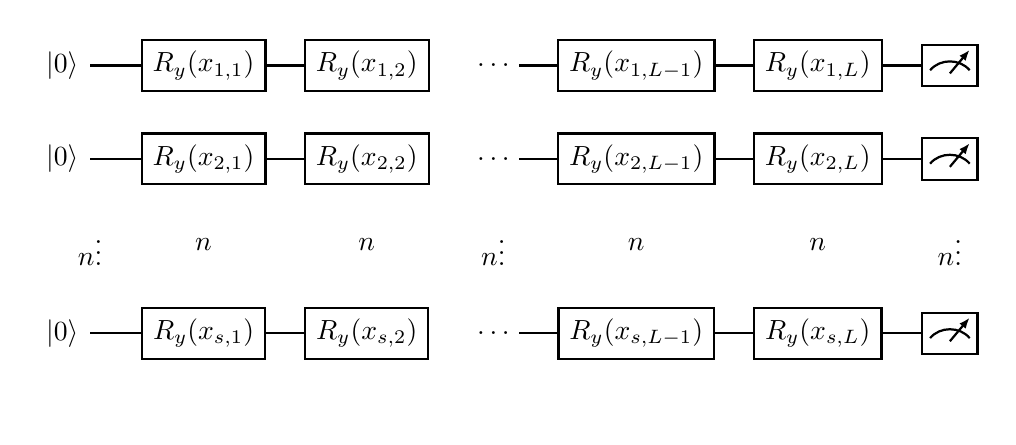
\begin{tikzpicture}
    \node[scale=1]{
        \begin{quantikz}
            \lstick{$\ket{0}$} & \gate{R_y(x_{1,1})}    & \gate{R_y(x_{1,2})}    &\ \ldots\ & \gate{R_y(x_{1,L-1})}    & \gate{R_y(x_{1,L})}& \meter{} \\
            \lstick{$\ket{0}$} & \gate{R_y(x_{2,1})}    & \gate{R_y(x_{2,2})}    &\ \ldots\ & \gate{R_y(x_{2,L-1})}    & \gate{R_y(x_{2,L})}& \meter{} \\
            \wn\vdots&\wn&\wn&\wn\vdots&\wn&\wn&\wn\vdots\\
            \lstick{$\ket{0}$} & \gate{R_y(x_{s,1})}    & \gate{R_y(x_{s,2})}    &\ \ldots\ & \gate{R_y(x_{s,L-1})}    & \gate{R_y(x_{s,L})}& \meter{}\\
        \end{quantikz}};
    \end{tikzpicture}
    \caption{$s$ 量子ビットからなる量子回路。$L$ 層の $R_y$ ゲートからなる。}
    \label{fig:circuit-concentration-1_}
\end{figure}

\begin{proof}
    回路の構造上、データ入力後の状態はエンタングルメントを持たないので、$\rho(\bs{x}) = \rho(\bs{x}_1) \otimes \rho(\bs{x}_2) \otimes \cdots \otimes \rho(\bs{x}_s)$ と表せる。また、$R_y$ のみを用いているから、$\rho(\bs{x}_j) = R_y(x_{j,1} + x_{j,2} + \cdots + x_{j,L})\dyad{0}R_y\dg(x_{j,1} + x_{j,2} + \cdots + x_{j,L})$ である。
    入力データの成分は独立であるから、
    \begin{align}
        \E_\calX[\rho(\bs{x})] = \E_\calX[\rho(\bs{x}_1)] \otimes \E_\calX[\rho(\bs{x}_2)] \otimes \cdots \otimes \E_\calX[\rho(\bs{x}_s)]
    \end{align}
    が成り立つ。$\calZ$ についても同様。
    $\calX$ と $\calZ$ のデータセットのサイズの比率が $|\calX|:|\calZ| = p:q$ なので、
    $\bar{\rho} = \bar{\rho}_+ - \bar{\rho}_-$ は次で与えられる。
    \begin{align}
        \bar{\rho}
        &= p\E_\calX[\rho(\bs{x})] - q\E_\calZ[\rho(\bs{z})]\\
        &= p\bigotimes_{j=1}^s \E_\calX[\rho(\bs{x}_j)] - q\bigotimes_{j=1}^s \E_\calZ[\rho(\bs{z}_j)]\\
        &=: p\bigotimes_{j=1}^s \bar{\rho}_{x|j} - q\bigotimes_{j=1}^s \bar{\rho}_{z|j}
    \end{align}
    
    よって、$\Tr[(\bar{\rho})^2]$ は次のように書き換えられる。
    \begin{align}
        \Tr[(\bar{\rho})^2]
        &= \Tr\qty[\qty(p\bigotimes_{j=1}^s \bar{\rho}_{x|j} - q\bigotimes_{j=1}^s \bar{\rho}_{z|j})^2]\\
        &= p^2\Tr\qty[\qty(\bigotimes_{j=1}^s \bar{\rho}_{x|j})^2] + q^2\Tr\qty[\qty(\bigotimes_{j=1}^s \bar{\rho}_{z|j})^2] - 2pq\Tr\qty[\qty(\bigotimes_{j=1}^s \bar{\rho}_{x|j}\bar{\rho}_{z|j})]\\
        &= p^2\prod_{j=1}^s\Tr[(\bar{\rho}_{x|j})^2] + q^2\prod_{j=1}^s\Tr[(\bar{\rho}_{z|j})^2] - 2pq\prod_{j=1}^s\Tr[\bar{\rho}_{x|j}\bar{\rho}_{z|j}]
    \end{align}
    
    $X_j = \sum_{d=1}^L x_{j,d}$ として $\bar{\rho}_{x|j}$ の行列は次で与えられる。
    \begin{align}
        \bar{\rho}_{x|j}
        = \frac12\mqty[1 + \E[\cos(X_j)] & \E[\sin(X_j)] \\
                        \E[\sin(X_j)] & 1 - \E[\cos(X_j)]]
    \end{align}
    
    これより、
    \begin{align}
        \Tr[(\bar{\rho}_{x|j})^2]
        &= \frac12\qty[1 + \E^2[\cos(X_j)] + \E^2[\sin(X_j)]]
    \end{align}
    ここで、補題~\ref{lem:cos-sin-expectation}と $X_j \sim \calN(\sum_{d=1}^L \mu_{x|j,d}, \sum_{d=1}^L \sigma_{x|j,d}^2)$ であることから、$\Sigma_{x|j}:=\sum_{d=1}^L \sigma_{x|j,d}^2$ とおくと、
    \begin{align}
        \Tr[(\bar{\rho}_{x|j})^2]
        &= \frac12\qty[1 + e^{-\Sigma_{x|j}}\cos^2\qty(\sum\nolimits_{d=1}^L \mu_{x|j,d}) + e^{-\Sigma_{x|j}}\sin^2\qty(\sum\nolimits_{d=1}^L \mu_{x|j,d})]\nonumber\\
        &= \frac12\qty(1 + e^{-\Sigma_{x|j}})
    \end{align}
    
    同様に $Z_j = \sum_{d=1}^L z_{j,d}$, $\Sigma_{z|j}:=\sum_{d=1}^L \sigma_{z|j,d}^2$ とすると、$\Tr[(\bar{\rho}_{z|j})^2]$ は次のようになる。
    \begin{align}
        \Tr[(\bar{\rho}_{z|j})^2]
        &= \frac12\qty(1 + e^{-\Sigma_{z|j}})
    \end{align}

    また、$\Tr[\bar{\rho}_{x|j}\bar{\rho}_{z|j}]$ は次のようになる。    
    \begin{align}
        \Tr[\bar{\rho}_{x|j}\bar{\rho}_{z|j}]
        &= \frac12\qty[1 + \E[\cos(X_j)]\E[\cos(Z_j)] + \E[\sin(X_j)]\E[\sin(Z_j)]]\nonumber\\
        &= \frac12\qty[1 + e^{-(\Sigma_{x|j}+\Sigma_{z|j})/2}\cos\qty(\sum\nolimits_j \mu_{x|j,d} - \sum\nolimits_j \mu_{z|j,d})]
    \end{align}
    
    これより、$\Tr[(\bar{\rho}_{x|j}\bar{\rho}_{z|j})]$ は次の不等式を満たす。
    \begin{align}
        \frac12\qty(1 - e^{-(\Sigma_{x|j}+\Sigma_{z|j})/2})
        \leq \Tr[(\bar{\rho}_{x|j}\bar{\rho}_{z|j})]
        \leq \frac12\qty(1 + e^{-(\Sigma_{x|j}+\Sigma_{z|j})/2})
    \end{align}
    
    したがって、$\Tr[(\bar{\rho})^2]$ は、次の不等式を満たす。
    \begin{align}\label{eq:ineq-1}
        \frac{1}{2^s}
        \qty[
            p^2\prod_{j=1}^s(1 + e^{-\Sigma_{x|j}})
            + q^2\prod_{j=1}^s(1 + e^{-\Sigma_{z|j}})
            - 2pq\prod_{j=1}^s(1 + e^{-(\Sigma_{x|j}+\Sigma_{z|j})/2})
        ]
        \leq \Tr[(\bar{\rho})^2]\nonumber\\
        \leq
        \frac{1}{2^s}
        \qty[
            p^2\prod_{j=1}^s\qty(1 + e^{-\Sigma_{x|j}})
            + q^2\prod_{j=1}^s\qty(1 + e^{-\Sigma_{z|j}})
            - 2pq\prod_{j=1}^s\qty(1 - e^{-(\Sigma_{x|j}+\Sigma_{z|j})/2})
        ]
    \end{align}
    
    不等式~\eqref{eq:ineq-1}の左辺の展開した各項について次が成り立つ。$(1 \leq j_p \leq s)$
    \begin{align}
        &p^2 \cdot 1^{s-t} \prod_{p=1}^{t}e^{-\Sigma_{x|j_p}}
        + q^2 \cdot 1^{s-t} \prod_{p=1}^{t}e^{-\Sigma_{z|j_p}}
        - 2pq \cdot 1^{s-t} \prod_{p=1}^{t}e^{-(\Sigma_{x|j_p}+\Sigma_{z|j_p})/2}\\
        &=
        \qty(p\prod_{p=1}^{t}e^{-\Sigma_{x|j_p}/2} - q\prod_{p=1}^{t}e^{-\Sigma_{z|j_p}/2})^2
        \geq 0
    \end{align}
    
    この不等式より、不等式~\eqref{eq:ineq-1}の左辺は次の式で下から抑えられる。
    \begin{align}
        &\frac{1}{2^s}
        \qty[
            p^2\prod_{j=1}^s(1 + e^{-\Sigma_{x|j}})
            + q^2\prod_{j=1}^s(1 + e^{-\Sigma_{z|j}})
            - 2pq\prod_{j=1}^s(1 + e^{-(\Sigma_{x|j}+\Sigma_{z|j})/2})
        ]\\
        \geq
        &\frac{1}{2^s}
        \Big[
            p^2(1 + e^{-\Sigma_{x|1}} + e^{-\Sigma_{x|2}} + \cdots + e^{-\Sigma_{x|s}})
            + q^2(1 + e^{-\Sigma_{z|1}} + e^{-\Sigma_{z|2}} + \cdots + e^{-\Sigma_{z|s}})\nonumber\\
            &\qquad\qquad- 2pq(1 + e^{-(\Sigma_{x|1}+\Sigma_{z|1})/2} + e^{-(\Sigma_{x|2}+\Sigma_{z|2})/2} + \cdots + e^{-(\Sigma_{x|s}+\Sigma_{z|s})/2})
        \Big]\\
        &=
        \frac{1}{2^s}
        \qty[(p-q)^2 + \sum_{j=1}^s \qty(p\,e^{-\Sigma_{x|j}/2} - q\,e^{-\Sigma_{z|j}/2})^2]
    \end{align}
    
    また、$L\,\sigma_{\min} \leq \Sigma_{x|j},\, \Sigma_{z|j}$ により、不等式~\eqref{eq:ineq-1}の右辺は次の式で上から抑えられる。
    \begin{align}
        &\frac{1}{2^s}
        \qty[
            p^2\prod_{j=1}^s(1 + e^{-\Sigma_{x|j}})
            + q^2\prod_{j=1}^s(1 + e^{-\Sigma_{z|j}})
            - 2pq\prod_{j=1}^s(1 - e^{-(\Sigma_{x|j}+\Sigma_{z|j})/2})
        ]\\
        &\leq
        \frac{1}{2^s} (1 + e^{-L\,\sigma_{\min}^2})^s
    \end{align}
    
    以上より、$w = p-q$ として $\Tr[(\bar{\rho})^2]$ は上下から次の式で抑えられる。
    \begin{align}
        \frac{1}{2^s}
        \qty[w^2 + \sum_{j=1}^s \qty(p\,e^{-\Sigma_{x|j}/2} - q\,e^{-\Sigma_{z|j}/2})^2]
        \leq \Tr[(\bar{\rho})^2]
        \leq \frac{1}{2^s} (1 + e^{-L\,\sigma_{\min}^2})^s
    \end{align}
\end{proof}



\begin{comment}
\begin{proof}
    回路の構造上、データ入力後の状態はエンタングルメントを持たないので、$\rho(\bs{x}) = \rho(\bs{x}_1) \otimes \rho(\bs{x}_2) \otimes \cdots \otimes \rho(\bs{x}_s)$ と表せる。また、$R_y$ のみを用いているから、$\rho(\bs{x}_j) = R_y(x_{j,1} + x_{j,2} + \cdots + x_{j,L})\dyad{0}R_y\dg(x_{j,1} + x_{j,2} + \cdots + x_{j,L})$ である。
    入力データの成分は独立であるから、
    \begin{align}
        \E_\calX[\rho(\bs{x})] = \E_\calX[\rho(\bs{x}_1)] \otimes \E_\calX[\rho(\bs{x}_2)] \otimes \cdots \otimes \E_\calX[\rho(\bs{x}_s)]
    \end{align}
    が成り立つ。$\calZ$ についても同様。
    $\calX$ と $\calZ$ のデータセットのサイズの比率が $|\calX|:|\calZ| = p:q$ なので、
    $\bar{\rho} = \bar{\rho}_+ - \bar{\rho}_-$ は次で与えられる。
    \begin{align}
        \bar{\rho}
        &= p\E_\calX[\rho(\bs{x})] - q\E_\calZ[\rho(\bs{z})]\\
        &= \bigotimes_{j=1}^s \qty(p\E_\calX[\rho(\bs{x}_j)] - q\E_\calZ[\rho(\bs{z}_j)])\\
        &=: \bigotimes_{j=1}^s \bar{\rho}_j
    \end{align}
    
    $X_j = \sum_{d=1}^L x_{j,d},\, Z_j = \sum_{d=1}^L z_{j,d}$ として $\E_\calX[\rho(\bs{x}_j)]$ の行列は次のようになる。
    \begin{align}
        \E_\calX[\rho(\bs{x}_j)]
        = \frac12\mqty[1 + \E[\cos(X_j)] & \E[\sin(X_j)] \\
                        \E[\sin(X_j)] & 1 - \E[\cos(X_j)]]
    \end{align}

    ゆえに、$\bar{\rho}_j$ は次のようになる。
    \begin{align}
        \bar{\rho}_j
        &= p\E[\rho(\bs{x}_j)] - q\E[\rho(\bs{z}_j)]\\
        &=
        \frac12\mqty[(p-q) + p\E[\cos(X_j)] - q\E[\cos(Z_j)] & p\E[\sin(X_j)] - q\E[\sin(Z_j)] \\
        p\E[\sin(X_j)] - q\E[\sin(Z_j)] & (p-q) - p\E[\cos(X_j)] + q\E[\cos(Z_j)]]
    \end{align}
    
    これより
    \begin{align}
        \Tr[(\bar{\rho}_j)^2]
        &= \frac12\Big[w^2 + \qty(p\E[\cos(X_j)] - q\E[\cos(Z_j)])^2 + \qty(p\E[\sin(X_j)] - q\E[\sin(Z_j)])^2\Big]\\
        &= \frac12\Big[w^2 + p^2\qty(\E^2[\cos(X_j)] + \E^2[\sin(X_j)]) + q^2\qty(\E[\cos(Z_j)]^2 + \E[\sin(Z_j)]^2)\nonumber\\
        &\qquad- 2pq\qty(\E[\cos(X_j)]\E[\cos(Z_j)] + \E[\sin(X_j)]\E[\sin(Z_j)])\Big]
    \end{align}
    
    ここで、補題~\ref{lem:cos-sin-expectation}と $X_j \sim \calN(\sum_{d=1}^L \mu_{x|j,d}, \sum_{d=1}^L \sigma_{x|j,d}^2)$ であることから、$w = p - q$, $\Sigma_{x|j}:=\sum_{d=1}^L \sigma_{x|j,d}^2$, $\Sigma_{z|j}:=\sum_{d=1}^L \sigma_{z|j,d}^2$ とおくと、
    \begin{align}
        \Tr[(\bar{\rho}_j)^2]
        = \frac12\Big[w^2 &+ p^2e^{-\Sigma_{x|j}} + q^2e^{-\Sigma_{z|j}}\nonumber\\
        &- 2pq\,e^{-(\Sigma_{x|j}+\Sigma_{z|j})/2}\cos(\sum\nolimits_j \mu_{x|j,d} - \sum\nolimits_j \mu_{z|j,d})\Big]
    \end{align}
    
    この表式と、$\sigma_{\min} \leq \sigma_{x|\fa j,d},\, \sigma_{z|\fa j,d}$ により、$\Tr[(\bar{\rho}_j)^2]$ を次のように上から抑えることができる。
    \begin{align}
        \Tr[(\bar{\rho}_j)^2]
        &\leq \frac12\Big[w^2 + p^2e^{-\Sigma_{x|j}} + q^2e^{-\Sigma_{z|j}} + 2pq\,e^{-(\Sigma_{x|j}+\Sigma_{z|j})/2}\Big]\\
        &= \frac12\Big[w^2 + (p\,e^{-\Sigma_{x|j}/2} + q\,e^{-\Sigma_{z|j}/2})^2\Big]\\
        &\leq \frac12\Big[w^2 + (p\,e^{-L\,\sigma_{\min}^2/2} + q\,e^{-L\,\sigma_{\min}^2/2})^2\Big]\\
        &= \frac12\Big[w^2 + e^{-L\,\sigma_{\min}^2}\Big]
    \end{align}
    
    また、$\Tr[(\bar{\rho}_j)^2]$ を下から抑えることもできる。
    \begin{align}
        \Tr[(\bar{\rho}_j)^2]
        &\geq \frac12\Big[w^2 + p^2e^{-\Sigma_{x|j}} + q^2e^{-\Sigma_{z|j}} - 2pq\,e^{-(\Sigma_{x|j}+\Sigma_{z|j})/2}\Big]\\
        &= \frac12\Big[w^2 + (p\,e^{-\Sigma_{x|j}/2} - q\,e^{-\Sigma_{z|j}/2})^2\Big]
    \end{align}
    
    これと、$|\calX|:|\calZ| = p:q$ であることから
    $\Tr[(\bar{\rho}_j)^2]$ について次の不等式が成り立つ。
    \begin{align}
        \frac12\qty[w^2 + \qty(p\,e^{-\Sigma_{x|j}/2} - q\,e^{-\Sigma_{z|j}/2})^2]
        \leq \Tr[(\bar{\rho}_j)^2]
        \leq \frac12\qty[w^2 + e^{-L\,\sigma_{\min}^2}]
    \end{align}
    したがって、$\bar{\rho} = \bigotimes_{j=1}^s \bar{\rho}_j$ は次の不等式を満たす。
    \begin{align}
        \frac{1}{2^s}
        \prod_{j=1}^s
        \qty[w^2
            + \qty(p\,e^{-\Sigma_{x|j}/2}- q\,e^{-\Sigma_{z|j}/2})^2
        ]
        \leq \Tr[(\bar{\rho})^2]
        \leq \frac{1}{2^s} \qty[w^2 + e^{-L\,\sigma_{\min}^2}]^s
    \end{align}
\end{proof}
\end{comment}



\section{定理\ref{thm:concentration-2}の略証}\label{sec:prf-concentration-2}
\begin{screen}
    \begin{theorem}
        (論文~\cite{li2022concentration}の Theorem 2 の拡張された結果)
        $\calX = \{\bs{x}\}$ はラベル $y_i=0$ に属する入力データセットであるとする。
        そして、各データサンプルを次のように表記する:$\bs{x} = (\bs{x}_{j})_{j=1}^s,\, \bs{x}_{j} = (\bs{x}_{j,d})_{d=1}^L,\,\bs{x}_{j,d} = (x_{j,d,1},x_{j,d,2},x_{j,d,3})$。
        入力データの各成分の分布は $x_{j,d,k} \sim \calN(\mu_{x|j,d,k}, \sigma_{x|j,d,k}^2)$ であり、分散は $\sigma_{\min} \leq \sigma_{x|\fa j,d} \leq \sigma_{\max}$ を満たすとする。また、入力回路は次の図~\ref{fig:circuit-concentration-2_}のように構成されているとする。ただし、$1\leq j\leq s,\, 1\leq d\leq L,\,1\leq k\leq 3$ である。
        このとき、$\bar{\rho} := \E_\calX[\rho(\bs{x})]$ について次の不等式が成り立つ。
        \begin{align}
            \frac{1}{2^s} + e^{-3s\,L\,\sigma_{\max}^2}
            \leq \Tr[(\bar{\rho})^2]
            \leq \frac{1}{2^s} + e^{-L\,\sigma_{\min}^2}
        \end{align}
        ただし、$s$ は量子ビット数、$L$ は入力回路の層数である。論文内では、$s = n,\,L = D$ である。
    \end{theorem}
\end{screen}

\begin{figure}[H]
    \centering
    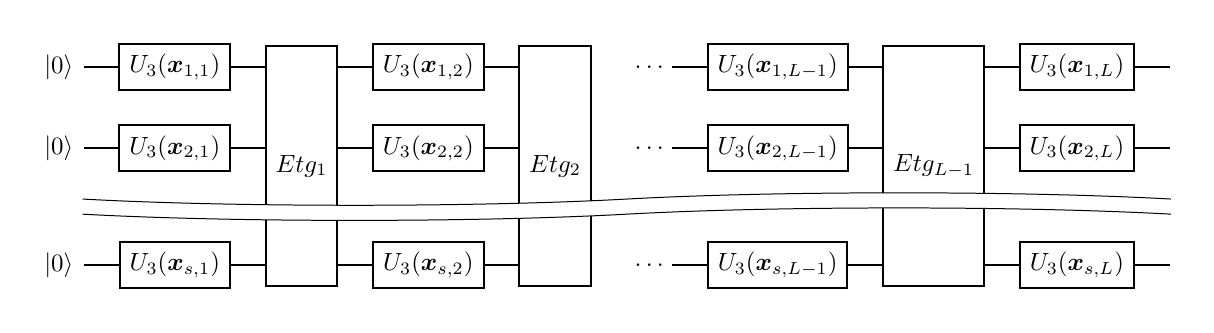
\begin{tikzpicture}
    \node[scale=0.9]{
        \begin{quantikz}
            \lstick{$\ket{0}$} & \gate{U_3(\bs{x}_{1,1})}    &\gate[4]{Etg_{1}}& \gate{U_3(\bs{x}_{1,2})}&\gate[4]{Etg_{2}}&\ \ldots\ & \gate{U_3(\bs{x}_{1,L-1})}&\gate[4]{Etg_{L-1}}& \gate{U_3(\bs{x}_{1,L})} & \qw \\
            \lstick{$\ket{0}$} & \gate{U_3(\bs{x}_{2,1})}    & \qw           & \gate{U_3(\bs{x}_{2,2})}    & \qw           &\ \ldots\ & \gate{U_3(\bs{x}_{2,L-1})}    & \qw               & \gate{U_3(\bs{x}_{2,L})}   & \qw \\
            \wave&&&&&&&&&\\
            \lstick{$\ket{0}$} & \gate{U_3(\bs{x}_{s,1})}    & \qw           & \gate{U_3(\bs{x}_{s,2})}    & \qw           &\ \ldots\ & \gate{U_3(\bs{x}_{s,L-1})}    & \qw               & \gate{U_3(\bs{x}_{s,L})}   & \qw
        \end{quantikz}};
    \end{tikzpicture}
    \caption{$s$ 量子ビットからなる量子回路。入力回路は、データを入力する $U_3(\bs{x}_{j,d})$ ゲートの $L$ 層と、 CNOT ゲートや CZ ゲートによってエンタングルメントを生成する層 $Etg_{d\prm}$ の $L-1$ 層からなる。ただし、$1\leq j\leq s,\, 1\leq d\leq L,\, 1\leq d\prm\leq L-1$ である。}
    \label{fig:circuit-concentration-2_}
\end{figure}


\begin{proof}\label{prf:concentration-2}
    論文~\cite{li2022concentration}内の式(S53)における $s_m^2$ の固有値が $e^{-\sigma_{\min}^2}$ を超えないことと同様に、$e^{-2\,\sigma_{\max}^2} \leq A_2^2A_3^2$ かつ $e^{-\,\sigma_{\max}^2/2} \leq A_1$ であることから $e^{-3\sigma_{\max}^2}$ を下回らないことがわかる。よって、$\bigotimes_{j=1}^s T_{j,d}$ の固有値は $e^{-3s\,\sigma_{\max}^2}$ を下回らない。
    \begin{align}
        \Tr[(\bar{\rho})^2] = \frac{1}{2^s} + 2^s\stackrel{\circ}{\pi}_0 \calT_1 \calE_1 \cdots \calT_{L-1} \calE_{L-1} \calT_L \calT_L^{\top} \calE_{L-1}^{\top} \calT_{L-1}^{\top} \cdots \calE_1^{\top} \calT_1^{\top} \stackrel{\circ}{\pi}_0^{\top}
    \end{align}
    であり、第二項は次のように上から抑えられる。
    \begin{align}
        \stackrel{\circ}{\pi}_0 \calT_1 \calE_1 \cdots \calT_{L-1} \calE_{L-1} \calT_L \calT_L^{\top} \calE_{L-1}^{\top} \calT_{L-1}^{\top} \cdots \calE_1^{\top} \calT_1^{\top} \stackrel{\circ}{\pi}_0^{\top}
        \leq \abs{\stackrel{\circ}{\pi}_0}_2^2 e^{-L \sigma_{\min}^2}
        = \frac{2^s-1}{2^{2s}} e^{-L \sigma_{\min}^2}
        \leq \frac{e^{-L \sigma_{\min}^2}}{2^s}
    \end{align}
    同様に、第二項は次のように下から抑えられる。
    \begin{align}
        \frac{e^{-3sL \sigma_{\max}^2}}{2^s} \leq \frac{2^s-1}{2^{2s}} e^{-3sL\,\sigma_{\max}^2} \leq \abs{\stackrel{\circ}{\pi}_0}_2^2 e^{-3sL \sigma_{\max}^2} \leq \stackrel{\circ}{\pi}_0 \calT_1 \calE_1 \cdots \calT_{L-1} \calE_{L-1} \calT_L \calT_L^{\top} \calE_{L-1}^{\top} \calT_{L-1}^{\top} \cdots \calE_1^{\top} \calT_1^{\top} \stackrel{\circ}{\pi}_0^{\top}
    \end{align}
    ゆえに、拡張された定理を得る。
\end{proof}

\end{document}